% Options for packages loaded elsewhere
\PassOptionsToPackage{unicode}{hyperref}
\PassOptionsToPackage{hyphens}{url}
%
\documentclass[
  12pt,
]{book}
\usepackage{amsmath,amssymb}
\usepackage{lmodern}
\usepackage{iftex}
\ifPDFTeX
  \usepackage[T1]{fontenc}
  \usepackage[utf8]{inputenc}
  \usepackage{textcomp} % provide euro and other symbols
\else % if luatex or xetex
  \usepackage{unicode-math}
  \defaultfontfeatures{Scale=MatchLowercase}
  \defaultfontfeatures[\rmfamily]{Ligatures=TeX,Scale=1}
\fi
% Use upquote if available, for straight quotes in verbatim environments
\IfFileExists{upquote.sty}{\usepackage{upquote}}{}
\IfFileExists{microtype.sty}{% use microtype if available
  \usepackage[]{microtype}
  \UseMicrotypeSet[protrusion]{basicmath} % disable protrusion for tt fonts
}{}
\makeatletter
\@ifundefined{KOMAClassName}{% if non-KOMA class
  \IfFileExists{parskip.sty}{%
    \usepackage{parskip}
  }{% else
    \setlength{\parindent}{0pt}
    \setlength{\parskip}{6pt plus 2pt minus 1pt}}
}{% if KOMA class
  \KOMAoptions{parskip=half}}
\makeatother
\usepackage{xcolor}
\usepackage{color}
\usepackage{fancyvrb}
\newcommand{\VerbBar}{|}
\newcommand{\VERB}{\Verb[commandchars=\\\{\}]}
\DefineVerbatimEnvironment{Highlighting}{Verbatim}{commandchars=\\\{\}}
% Add ',fontsize=\small' for more characters per line
\usepackage{framed}
\definecolor{shadecolor}{RGB}{248,248,248}
\newenvironment{Shaded}{\begin{snugshade}}{\end{snugshade}}
\newcommand{\AlertTok}[1]{\textcolor[rgb]{0.94,0.16,0.16}{#1}}
\newcommand{\AnnotationTok}[1]{\textcolor[rgb]{0.56,0.35,0.01}{\textbf{\textit{#1}}}}
\newcommand{\AttributeTok}[1]{\textcolor[rgb]{0.77,0.63,0.00}{#1}}
\newcommand{\BaseNTok}[1]{\textcolor[rgb]{0.00,0.00,0.81}{#1}}
\newcommand{\BuiltInTok}[1]{#1}
\newcommand{\CharTok}[1]{\textcolor[rgb]{0.31,0.60,0.02}{#1}}
\newcommand{\CommentTok}[1]{\textcolor[rgb]{0.56,0.35,0.01}{\textit{#1}}}
\newcommand{\CommentVarTok}[1]{\textcolor[rgb]{0.56,0.35,0.01}{\textbf{\textit{#1}}}}
\newcommand{\ConstantTok}[1]{\textcolor[rgb]{0.00,0.00,0.00}{#1}}
\newcommand{\ControlFlowTok}[1]{\textcolor[rgb]{0.13,0.29,0.53}{\textbf{#1}}}
\newcommand{\DataTypeTok}[1]{\textcolor[rgb]{0.13,0.29,0.53}{#1}}
\newcommand{\DecValTok}[1]{\textcolor[rgb]{0.00,0.00,0.81}{#1}}
\newcommand{\DocumentationTok}[1]{\textcolor[rgb]{0.56,0.35,0.01}{\textbf{\textit{#1}}}}
\newcommand{\ErrorTok}[1]{\textcolor[rgb]{0.64,0.00,0.00}{\textbf{#1}}}
\newcommand{\ExtensionTok}[1]{#1}
\newcommand{\FloatTok}[1]{\textcolor[rgb]{0.00,0.00,0.81}{#1}}
\newcommand{\FunctionTok}[1]{\textcolor[rgb]{0.00,0.00,0.00}{#1}}
\newcommand{\ImportTok}[1]{#1}
\newcommand{\InformationTok}[1]{\textcolor[rgb]{0.56,0.35,0.01}{\textbf{\textit{#1}}}}
\newcommand{\KeywordTok}[1]{\textcolor[rgb]{0.13,0.29,0.53}{\textbf{#1}}}
\newcommand{\NormalTok}[1]{#1}
\newcommand{\OperatorTok}[1]{\textcolor[rgb]{0.81,0.36,0.00}{\textbf{#1}}}
\newcommand{\OtherTok}[1]{\textcolor[rgb]{0.56,0.35,0.01}{#1}}
\newcommand{\PreprocessorTok}[1]{\textcolor[rgb]{0.56,0.35,0.01}{\textit{#1}}}
\newcommand{\RegionMarkerTok}[1]{#1}
\newcommand{\SpecialCharTok}[1]{\textcolor[rgb]{0.00,0.00,0.00}{#1}}
\newcommand{\SpecialStringTok}[1]{\textcolor[rgb]{0.31,0.60,0.02}{#1}}
\newcommand{\StringTok}[1]{\textcolor[rgb]{0.31,0.60,0.02}{#1}}
\newcommand{\VariableTok}[1]{\textcolor[rgb]{0.00,0.00,0.00}{#1}}
\newcommand{\VerbatimStringTok}[1]{\textcolor[rgb]{0.31,0.60,0.02}{#1}}
\newcommand{\WarningTok}[1]{\textcolor[rgb]{0.56,0.35,0.01}{\textbf{\textit{#1}}}}
\usepackage{longtable,booktabs,array}
\usepackage{calc} % for calculating minipage widths
% Correct order of tables after \paragraph or \subparagraph
\usepackage{etoolbox}
\makeatletter
\patchcmd\longtable{\par}{\if@noskipsec\mbox{}\fi\par}{}{}
\makeatother
% Allow footnotes in longtable head/foot
\IfFileExists{footnotehyper.sty}{\usepackage{footnotehyper}}{\usepackage{footnote}}
\makesavenoteenv{longtable}
\usepackage{graphicx}
\makeatletter
\def\maxwidth{\ifdim\Gin@nat@width>\linewidth\linewidth\else\Gin@nat@width\fi}
\def\maxheight{\ifdim\Gin@nat@height>\textheight\textheight\else\Gin@nat@height\fi}
\makeatother
% Scale images if necessary, so that they will not overflow the page
% margins by default, and it is still possible to overwrite the defaults
% using explicit options in \includegraphics[width, height, ...]{}
\setkeys{Gin}{width=\maxwidth,height=\maxheight,keepaspectratio}
% Set default figure placement to htbp
\makeatletter
\def\fps@figure{htbp}
\makeatother
\setlength{\emergencystretch}{3em} % prevent overfull lines
\providecommand{\tightlist}{%
  \setlength{\itemsep}{0pt}\setlength{\parskip}{0pt}}
\setcounter{secnumdepth}{5}
\usepackage{booktabs}
\usepackage{amsthm}
\makeatletter
\def\thm@space@setup{%
  \thm@preskip=8pt plus 2pt minus 4pt
  \thm@postskip=\thm@preskip
}
\makeatother


%\usepackage[legalpaper, margin=1in]{geometry}

\usepackage[a4paper, total={6.5in, 9in}]{geometry}

\ifLuaTeX
  \usepackage{selnolig}  % disable illegal ligatures
\fi
\usepackage[]{natbib}
\bibliographystyle{apalike}
\IfFileExists{bookmark.sty}{\usepackage{bookmark}}{\usepackage{hyperref}}
\IfFileExists{xurl.sty}{\usepackage{xurl}}{} % add URL line breaks if available
\urlstyle{same} % disable monospaced font for URLs
\hypersetup{
  pdftitle={Introduction to Time Series},
  pdfauthor={Jean-Paul Renne},
  hidelinks,
  pdfcreator={LaTeX via pandoc}}

\title{Introduction to Time Series}
\author{Jean-Paul Renne}
\date{2023-02-17}

\usepackage{amsthm}
\newtheorem{theorem}{Theorem}[chapter]
\newtheorem{lemma}{Lemma}[chapter]
\newtheorem{corollary}{Corollary}[chapter]
\newtheorem{proposition}{Proposition}[chapter]
\newtheorem{conjecture}{Conjecture}[chapter]
\theoremstyle{definition}
\newtheorem{definition}{Definition}[chapter]
\theoremstyle{definition}
\newtheorem{example}{Example}[chapter]
\theoremstyle{definition}
\newtheorem{exercise}{Exercise}[chapter]
\theoremstyle{definition}
\newtheorem{hypothesis}{Hypothesis}[chapter]
\theoremstyle{remark}
\newtheorem*{remark}{Remark}
\newtheorem*{solution}{Solution}
\begin{document}
\maketitle

{
\setcounter{tocdepth}{1}
\tableofcontents
}
\newcommand{\bv}[1]{\mathbf{#1}}

\hypertarget{intro}{%
\chapter*{Introduction to Time Series}\label{intro}}

Time series constitute a prevalent data type in several disciplines, notably macroeconomics and finance. The modeling of time series is crucial for many purposes, including forecasting, understanding macroeconomic mechanisms, and risk assessment. This course proposes an introduction to time series analysis. It has been developed by \href{https://sites.google.com/site/jeanpaulrenne/home}{Jean-Paul Renne}.

Codes associated with this course are part of the \texttt{AEC} package, which is available on GitHub. To load a package from GitHub, you need to use function \texttt{install\_github} from the \texttt{devtools} package:

\begin{Shaded}
\begin{Highlighting}[]
\FunctionTok{install.packages}\NormalTok{(}\StringTok{"devtools"}\NormalTok{) }\CommentTok{\# in case you do not have that one.}
\FunctionTok{library}\NormalTok{(devtools)}
\FunctionTok{install\_github}\NormalTok{(}\StringTok{"jrenne/AEC"}\NormalTok{)}
\FunctionTok{library}\NormalTok{(AEC)}
\end{Highlighting}
\end{Shaded}

\textbf{Useful (R) links:}

\begin{itemize}
\item
  Download R:

  \begin{itemize}
  \tightlist
  \item
    R software: \url{https://cran.r-project.org} (the basic R software)
  \item
    RStudio: \url{https://www.rstudio.com} (a convenient R editor)
  \end{itemize}
\item
  Tutorials:

  \begin{itemize}
  \tightlist
  \item
    Rstudio: \url{https://dss.princeton.edu/training/RStudio101.pdf} (by Oscar Torres-Reyna)
  \item
    R: \url{https://cran.r-project.org/doc/contrib/Paradis-rdebuts_en.pdf} (by Emmanuel Paradis)
  \item
    My own tutorial: \url{https://jrenne.shinyapps.io/Rtuto_publiShiny/}
  \end{itemize}
\end{itemize}

\hypertarget{Intro}{%
\chapter{Basics}\label{Intro}}

\hypertarget{shocks-and-lag-operator}{%
\section{Shocks and lag operator}\label{shocks-and-lag-operator}}

A time series is an infinite sequence of random variables indexed by time: \(\{y_t\}_{t=-\infty}^{+\infty}=\{\dots, y_{-2},y_{-1},y_{0},y_{1},\dots,y_t,\dots\}\), \(y_i \in \mathbb{R}^k\). In practice, we only observe samples, typically: \(\{y_{1},\dots,y_T\}\).

Standard time series models are built using \textbf{shocks} that we will often denote by \(\varepsilon_t\). Typically, \(\mathbb{E}(\varepsilon_t)=0\). In many models, the shocks are supposed to be i.i.d., but there exist other (less restrictive) notions of shocks. In particular, the definition of many processes is based on white noises:

\begin{definition}[White noise]
\protect\hypertarget{def:whitenoise}{}\label{def:whitenoise}

The process \(\{\varepsilon_t\}_{t \in] -\infty,+\infty[}\) is a white noise if, for all \(t\):

\begin{enumerate}
\def\labelenumi{\alph{enumi}.}
\tightlist
\item
  \(\mathbb{E}(\varepsilon_t)=0\),
\item
  \(\mathbb{E}(\varepsilon_t^2)=\sigma^2<\infty\),
\item
  for all \(s\ne t\), \(\mathbb{E}(\varepsilon_t \varepsilon_s)=0\).
\end{enumerate}

\end{definition}

Another type of shocks that are commonly used are Martingale Difference Sequences:

\begin{definition}[Martingale Difference Sequence]
\protect\hypertarget{def:MDS}{}\label{def:MDS}The process \(\{\varepsilon_t\}_{t = -\infty}^{+\infty}\) is a martingale difference sequence (MDS) if \(\mathbb{E}(|\varepsilon_{t}|)<\infty\) and if, for all \(t\),
\[
\underbrace{\mathbb{E}_{t-1}(\varepsilon_{t})}_{\mbox{conditional on the past}}=0.
\]
\end{definition}

By definition, if \(y_t\) is a martingale, then \(y_{t}-y_{t-1}\) is a MDS.

\begin{example}[ARCH process]
\protect\hypertarget{exm:ARCH}{}\label{exm:ARCH}

The Autoregressive conditional heteroskedasticity process---studied in Section \ref{ARCHGARCH}---is an example of shock that satisfies the white noise and MDS definitions, but that is not i.i.d.:
\[
\varepsilon_{t} = \sigma_t \times z_{t},
\]
where \(z_t \sim i.i.d.\,\mathcal{N}(0,1)\) and \(\sigma_t^2 = w + \alpha \varepsilon_{t-1}^2\).

\begin{Shaded}
\begin{Highlighting}[]
\NormalTok{T }\OtherTok{\textless{}{-}} \DecValTok{500}
\NormalTok{w }\OtherTok{\textless{}{-}} \DecValTok{1}\NormalTok{; alpha }\OtherTok{\textless{}{-}}\NormalTok{ .}\DecValTok{98}
\NormalTok{all\_epsilon }\OtherTok{\textless{}{-}} \ConstantTok{NULL}\NormalTok{; epsilon\_1 }\OtherTok{\textless{}{-}} \DecValTok{0}
\ControlFlowTok{for}\NormalTok{(t }\ControlFlowTok{in} \DecValTok{1}\SpecialCharTok{:}\NormalTok{T)\{}
\NormalTok{  sigma }\OtherTok{\textless{}{-}} \FunctionTok{sqrt}\NormalTok{(w }\SpecialCharTok{+}\NormalTok{ alpha }\SpecialCharTok{*}\NormalTok{ epsilon\_1}\SpecialCharTok{\^{}}\DecValTok{2}\NormalTok{)}
\NormalTok{  epsilon }\OtherTok{\textless{}{-}}\NormalTok{ sigma }\SpecialCharTok{*} \FunctionTok{rnorm}\NormalTok{(}\DecValTok{1}\NormalTok{)}
\NormalTok{  all\_epsilon }\OtherTok{\textless{}{-}} \FunctionTok{c}\NormalTok{(all\_epsilon,epsilon)}
\NormalTok{  epsilon\_1 }\OtherTok{\textless{}{-}}\NormalTok{ epsilon}
\NormalTok{\}}
\FunctionTok{par}\NormalTok{(}\AttributeTok{plt=}\FunctionTok{c}\NormalTok{(.}\DecValTok{15}\NormalTok{,.}\DecValTok{95}\NormalTok{,.}\DecValTok{1}\NormalTok{,.}\DecValTok{95}\NormalTok{))}
\FunctionTok{plot}\NormalTok{(all\_epsilon,}\AttributeTok{type=}\StringTok{"l"}\NormalTok{,}\AttributeTok{lwd=}\DecValTok{2}\NormalTok{,}
     \AttributeTok{ylab=}\FunctionTok{expression}\NormalTok{(epsilon[t]),}\AttributeTok{xlab=}\StringTok{""}\NormalTok{)}
\end{Highlighting}
\end{Shaded}

\begin{figure}
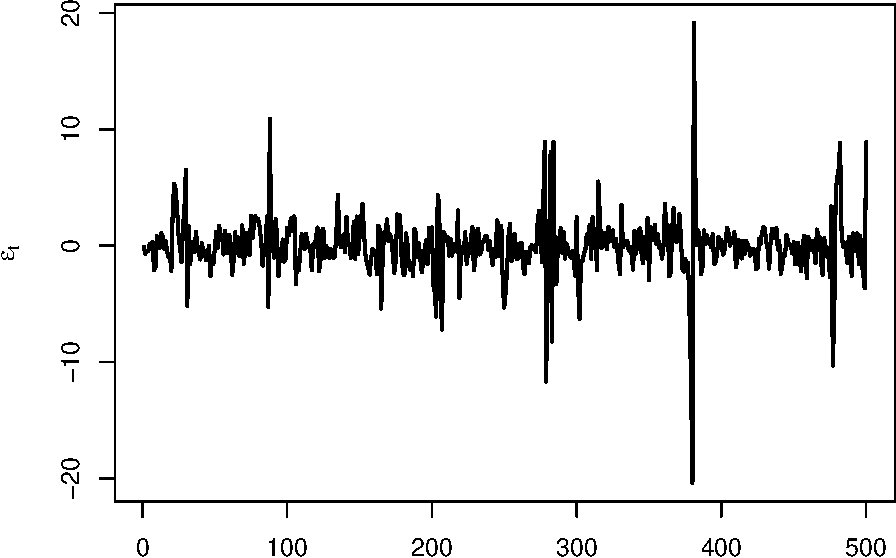
\includegraphics[width=0.95\linewidth]{TimeSeries_files/figure-latex/simulGARCHointro-1} \caption{Simulation of $\varepsilon_t$, where $\varepsilon_{t} = \sigma_t \times z_{t}$, with $z_t \sim i.i.d.\,\mathcal{N}(0,1)$.}\label{fig:simulGARCHointro}
\end{figure}

\end{example}

\begin{example}
\protect\hypertarget{exm:whiteNotMDS}{}\label{exm:whiteNotMDS}A white noise process is not necessarily a MDS. This is for instance the case for following process:
\[
\varepsilon_{t} = z_t + z_{t-1}z_{t-2},
\]
where \(z_t \sim i.i.d.\mathcal{N}(0,1)\).

Indeed, it can be shown that the \(\varepsilon_t\)'s are not correlated through time, we have \(\mathbb{E}_{t-1}(\varepsilon_t)=z_{t-1}z_{t-2} \ne 0\).
\end{example}

Let us now introduce the lag operator. The lag operator, denoted by \(L\), is defined on the time series space and is defined by:
\begin{equation}
L: \{y_t\}_{t=-\infty}^{+\infty} \rightarrow \{w_t\}_{t=-\infty}^{+\infty} \quad \mbox{with} \quad w_t = y_{t-1}.\label{eq:lagOp}
\end{equation}

It is easily seen that we have \(L^2 y_t =L(L y_t) = y_{t-2}\) and, more generally, \(L^k y_t = y_{t-k}\).

Consider a process \(y_t\) whose law of motion is \(y_t = \mu + \phi y_{t-1} + \varepsilon_t\), where the \(\varepsilon_t\)'s are i.i.d. \(\mathcal{N}(0,\sigma^2)\) (this is an AR(1) process, as we will see in Section \ref{Univariate}). Using the lag operator, the dynamics of \(y_t\) can be expressed as follows:
\[
(1-\phi L) y_t = \mu + \varepsilon_t.
\]

\hypertarget{conditional-and-unconditional-moments}{%
\section{Conditional and unconditional moments}\label{conditional-and-unconditional-moments}}

If it exists, the \textbf{unconditional (or marginal) mean} of the random variable \(y_t\) is given by:
\[
\mu_t := \mathbb{E}(y_t) = \int_{-\infty}^{\infty} y_t f_{Y_t}(y_t) dy_t,
\]
where \(f_{Y_t}\) is the unconditional, or marginal, density (p.d.f.) of \(y_t\). Note that, in the general case, \(Y_t\) and \(Y_{t-1}\), may have different densities; that is, in general, \(f_{Y_t} \ne f_{Y_{t-1}}\) (and, in particular, \(\mu_t \ne \mu_{t-1}\)).

Similarly, if it exists, the \textbf{unconditional (or marginal) variance} of the random variable \(y_t\) is:
\[
\mathbb{V}ar(y_t) = \int_{-\infty}^{\infty} (y_t - \mathbb{E}(y_t))^2 f_{Y_t}(y_t) dy_t.
\]

\begin{definition}[Autocovariance]
\protect\hypertarget{def:autocov}{}\label{def:autocov}The \(j^{th}\) autocovariance of \(y_t\) is given by:
\begin{eqnarray*}
\gamma_{j,t} &:=& \mathbb{E}([y_t - \mathbb{E}(y_t)][y_{t-j} - \mathbb{E}(y_{t-j})])\\
&=& \int_{-\infty}^{\infty} \int_{-\infty}^{\infty} \dots \int_{-\infty}^{\infty} [y_t - \mathbb{E}(y_t)][y_{t-j} - \mathbb{E}(y_{t-j})] \times\\
&& f_{Y_t,Y_{t-1},\dots,Y_{t-j}}(y_t,y_{t-1},\dots,y_{t-j}) dy_t dy_{t-1} \dots dy_{t-j},
\end{eqnarray*}
where \(f_{Y_t,Y_{t-1},\dots,Y_{t-j}}(y_t,y_{t-1},\dots,y_{t-j})\) is the joint distribution of \(y_t,y_{t-1},\dots,y_{t-j}\).
\end{definition}

In particular, note that \(\gamma_{0,t} = \mathbb{V}ar(y_t)\).

\begin{definition}[Covariance stationarity]
\protect\hypertarget{def:covstat}{}\label{def:covstat}The process \(y_t\) is covariance stationary ---or weakly stationary--- if, for all \(t\) and \(j\),
\[
\mathbb{E}(y_t) = \mu \quad \mbox{and} \quad \mathbb{E}\{(y_t - \mu)(y_{t-j} - \mu)\} = \gamma_j.
\]
\end{definition}

Figure \ref{fig:NONNstat1} displays the simulation of a process that is not covariance stationary. This process follows \(y_t = 0.1t + \varepsilon_t\), where \(\varepsilon_t \sim\,i.i.d.\,\mathcal{N}(0,1)\). Indeed, for such a process, we have: \(\mathbb{E}(y_t)=0.1t\), which depends on \(t\).

\begin{Shaded}
\begin{Highlighting}[]
\NormalTok{T }\OtherTok{\textless{}{-}} \DecValTok{200}
\NormalTok{y }\OtherTok{\textless{}{-}} \FloatTok{0.1}\SpecialCharTok{*}\NormalTok{(}\DecValTok{1}\SpecialCharTok{:}\NormalTok{T) }\SpecialCharTok{+} \FunctionTok{rnorm}\NormalTok{(T)}
\FunctionTok{par}\NormalTok{(}\AttributeTok{plt=}\FunctionTok{c}\NormalTok{(.}\DecValTok{1}\NormalTok{,.}\DecValTok{95}\NormalTok{,.}\DecValTok{1}\NormalTok{,.}\DecValTok{95}\NormalTok{))}
\FunctionTok{plot}\NormalTok{(y,}\AttributeTok{xlab=}\StringTok{""}\NormalTok{,}\AttributeTok{ylab=}\StringTok{""}\NormalTok{,}\AttributeTok{lwd=}\DecValTok{2}\NormalTok{,}\AttributeTok{type=}\StringTok{"l"}\NormalTok{)}
\end{Highlighting}
\end{Shaded}

\begin{figure}
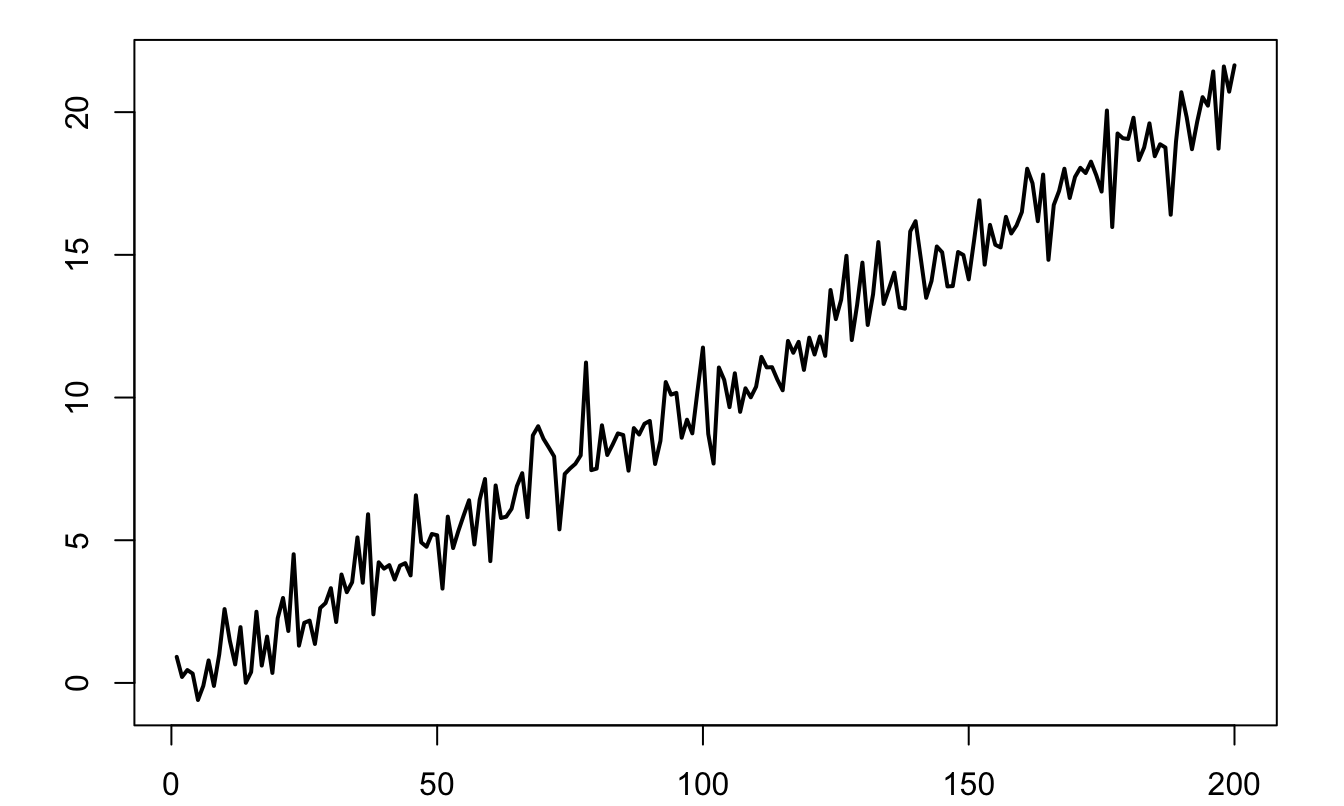
\includegraphics[width=0.95\linewidth]{TimeSeries_files/figure-latex/NONNstat1-1} \caption{Example of a process that is not covariance stationary. it follows: $y_t = 0.1t + \varepsilon_t$, where $\varepsilon_t \sim \mathcal{N}(0,1)$.}\label{fig:NONNstat1}
\end{figure}

\begin{definition}[Strict stationarity]
\protect\hypertarget{def:strictstat}{}\label{def:strictstat}The process \(y_t\) is strictly stationary if, for all \(t\) and all sets of integers \(J=\{j_1,\dots,j_n\}\), the distribution of \((y_{t},y_{t+j_1},\dots,y_{t+j_n})\) depends on \(J\) but not on \(t\).
\end{definition}

The following process is covariance stationary but not strictly stationary:
\[
y_t = \mathbb{I}_{\{t<1000\}}\varepsilon_{1,t}+\mathbb{I}_{\{t\ge1000\}}\varepsilon_{2,t},
\]
where \(\varepsilon_{1,t} \sim \mathcal{N}(0,1)\) and \(\varepsilon_{2,t} \sim \sqrt{\frac{\nu - 2}{\nu}} t(\nu)\) and \(\nu = 4\). A simulated path is displayed in Figure \ref{fig:NONNstat2}.

\begin{Shaded}
\begin{Highlighting}[]
\NormalTok{T }\OtherTok{\textless{}{-}} \DecValTok{2000}
\NormalTok{y }\OtherTok{\textless{}{-}} \FunctionTok{rnorm}\NormalTok{(T)}
\NormalTok{y[(T}\SpecialCharTok{/}\DecValTok{2}\NormalTok{)}\SpecialCharTok{:}\NormalTok{T] }\OtherTok{\textless{}{-}} \FunctionTok{rt}\NormalTok{(}\AttributeTok{n =}\NormalTok{ T}\SpecialCharTok{/}\DecValTok{2} \SpecialCharTok{+} \DecValTok{1}\NormalTok{,}\AttributeTok{df=}\DecValTok{4}\NormalTok{)}
\FunctionTok{par}\NormalTok{(}\AttributeTok{plt=}\FunctionTok{c}\NormalTok{(.}\DecValTok{1}\NormalTok{,.}\DecValTok{95}\NormalTok{,.}\DecValTok{15}\NormalTok{,.}\DecValTok{95}\NormalTok{))}
\FunctionTok{plot}\NormalTok{(y,}\AttributeTok{xlab=}\StringTok{""}\NormalTok{,}\AttributeTok{ylab=}\StringTok{""}\NormalTok{,}\AttributeTok{type=}\StringTok{"l"}\NormalTok{)}
\FunctionTok{abline}\NormalTok{(}\AttributeTok{h=}\SpecialCharTok{{-}}\FloatTok{2.58}\NormalTok{,}\AttributeTok{col=}\StringTok{"red"}\NormalTok{,}\AttributeTok{lty=}\DecValTok{3}\NormalTok{)}
\FunctionTok{abline}\NormalTok{(}\AttributeTok{h=}\FloatTok{2.58}\NormalTok{,}\AttributeTok{col=}\StringTok{"red"}\NormalTok{,}\AttributeTok{lty=}\DecValTok{3}\NormalTok{)}
\end{Highlighting}
\end{Shaded}

\begin{figure}
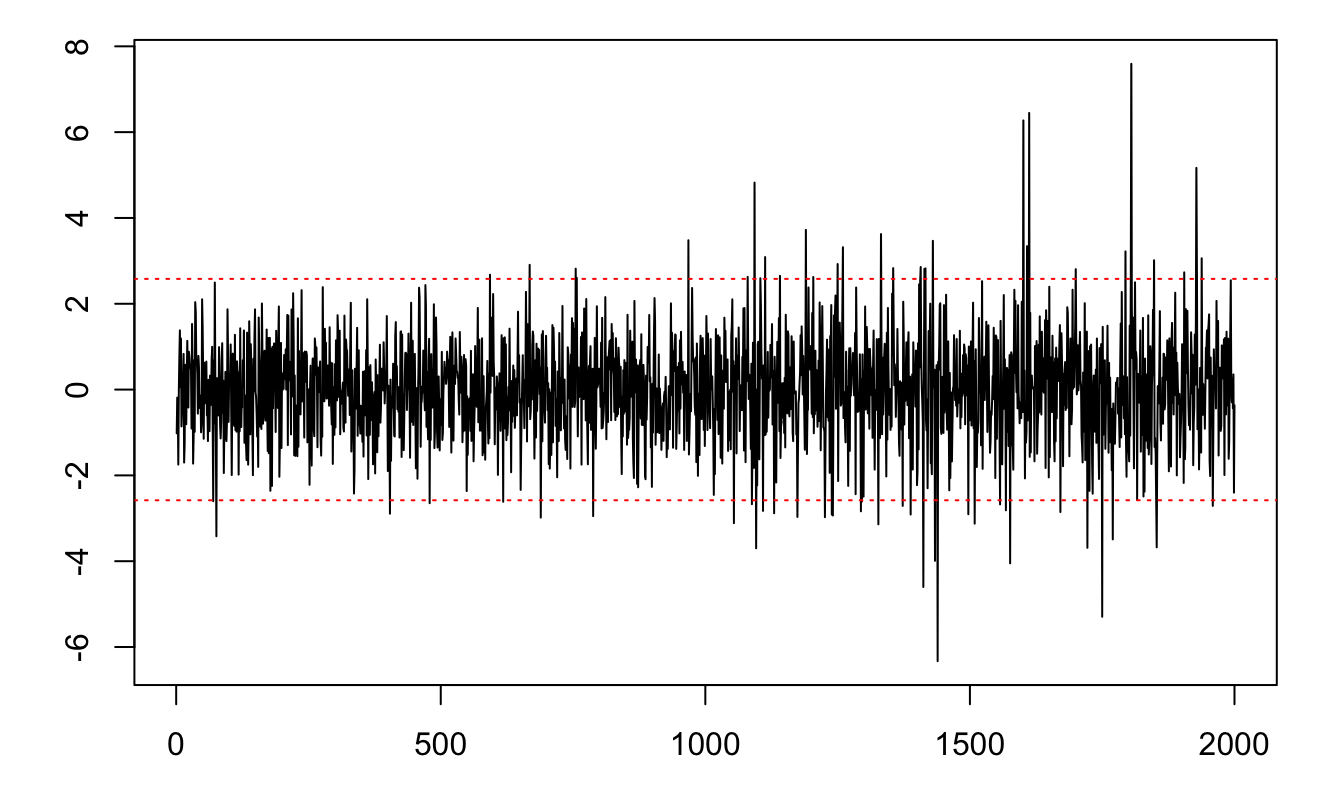
\includegraphics[width=0.95\linewidth]{TimeSeries_files/figure-latex/NONNstat2-1} \caption{Example of a process that is covariance stationary but not strictly stationary. The red lines delineate the 99\% confidence interval of the standard normal distribution ($\pm 2.58$).}\label{fig:NONNstat2}
\end{figure}

\begin{proposition}
\protect\hypertarget{prp:gammaMinus}{}\label{prp:gammaMinus}If \(y_t\) is covariance stationary, then \(\gamma_j = \gamma_{-j}\).
\end{proposition}

\begin{proof}
Since \(y_t\) is covariance stationary, the covariance between \(y_t\) and \(y_{t-j}\) (i.e., \(\gamma_j\)) is the same as that between \(y_{t+j}\) and \(y_{t+j-j}\) (i.e.~\(\gamma_{-j}\)).
\end{proof}

\begin{definition}[Auto-correlation]
\protect\hypertarget{def:autocor}{}\label{def:autocor}The \(j^{th}\) auto-correlation of a covariance-stationary process is:
\[
\rho_j = \frac{\gamma_j}{\gamma_0}.
\]
\end{definition}

Consider a long historical time series of the Swiss GDP growth, taken from the \citet{JST_2017} dataset.\footnote{Version 6 of the dataset, available on \href{https://www.macrohistory.net}{this website}.}

\begin{Shaded}
\begin{Highlighting}[]
\FunctionTok{library}\NormalTok{(AEC)}
\FunctionTok{data}\NormalTok{(JST);data }\OtherTok{\textless{}{-}} \FunctionTok{subset}\NormalTok{(JST,iso}\SpecialCharTok{==}\StringTok{"CHE"}\NormalTok{)}
\FunctionTok{par}\NormalTok{(}\AttributeTok{plt=}\FunctionTok{c}\NormalTok{(.}\DecValTok{1}\NormalTok{,.}\DecValTok{95}\NormalTok{,.}\DecValTok{1}\NormalTok{,.}\DecValTok{95}\NormalTok{))}
\NormalTok{T }\OtherTok{\textless{}{-}} \FunctionTok{dim}\NormalTok{(data)[}\DecValTok{1}\NormalTok{]}
\NormalTok{data}\SpecialCharTok{$}\NormalTok{growth }\OtherTok{\textless{}{-}} \FunctionTok{c}\NormalTok{(}\ConstantTok{NaN}\NormalTok{,}\FunctionTok{log}\NormalTok{(data}\SpecialCharTok{$}\NormalTok{gdp[}\DecValTok{2}\SpecialCharTok{:}\NormalTok{T]}\SpecialCharTok{/}\NormalTok{data}\SpecialCharTok{$}\NormalTok{gdp[}\DecValTok{1}\SpecialCharTok{:}\NormalTok{(T}\DecValTok{{-}1}\NormalTok{)]))}
\FunctionTok{plot}\NormalTok{(data}\SpecialCharTok{$}\NormalTok{year,data}\SpecialCharTok{$}\NormalTok{growth,}\AttributeTok{type=}\StringTok{"l"}\NormalTok{,}\AttributeTok{xlab=}\StringTok{""}\NormalTok{,}\AttributeTok{ylab=}\StringTok{""}\NormalTok{,}\AttributeTok{lwd=}\DecValTok{2}\NormalTok{)}
\FunctionTok{abline}\NormalTok{(}\AttributeTok{h=}\FunctionTok{mean}\NormalTok{(data}\SpecialCharTok{$}\NormalTok{growth,}\AttributeTok{na.rm =} \ConstantTok{TRUE}\NormalTok{),}\AttributeTok{col=}\StringTok{"blue"}\NormalTok{,}\AttributeTok{lty=}\DecValTok{2}\NormalTok{,}\AttributeTok{xlab=}\StringTok{""}\NormalTok{,}\AttributeTok{ylab=}\StringTok{""}\NormalTok{)}
\end{Highlighting}
\end{Shaded}

\begin{figure}
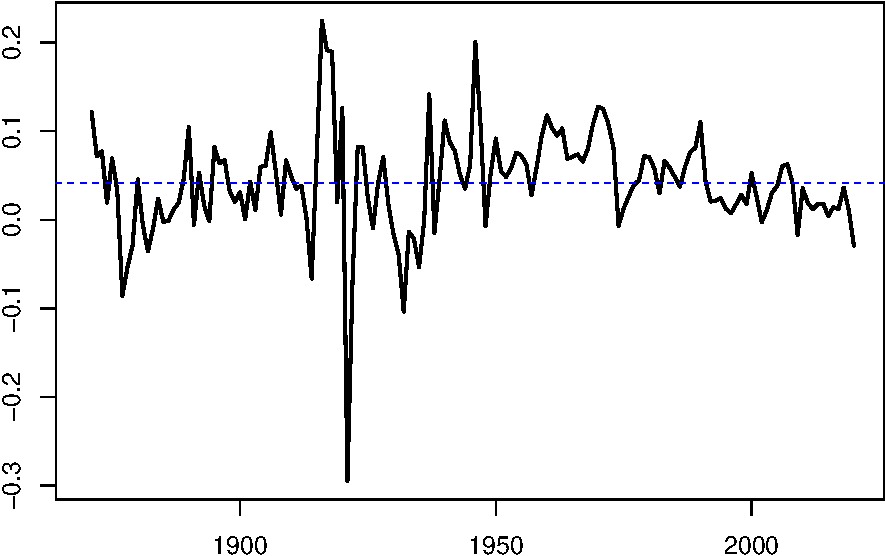
\includegraphics[width=0.95\linewidth]{TimeSeries_files/figure-latex/autocov-1} \caption{Annual growth rate of Swiss GDP, based on the Jorda-Schularick-Taylor Macrohistory Database.}\label{fig:autocov}
\end{figure}

Figure \ref{fig:autocov2} shows two scatter plots. In the first one, the coordinates of each point are of the form \((y_{t-1},y_t)\). Hence, the slope of the OLS regression line (in blue) is \(\widehat{\mathbb{C}ov}(y_t,y_{t-1})/\widehat{\mathbb{V}ar}(y_{t-1})\) (where the hats indicate that these moments are the sample ones). Assuming that the process is covariance stationary, the slope therefore is an estimate of the auto-correlation of order one. By the same logic, the slope of the blue line in the second plot is an estimate of the auto-correlation of order three.

\begin{figure}
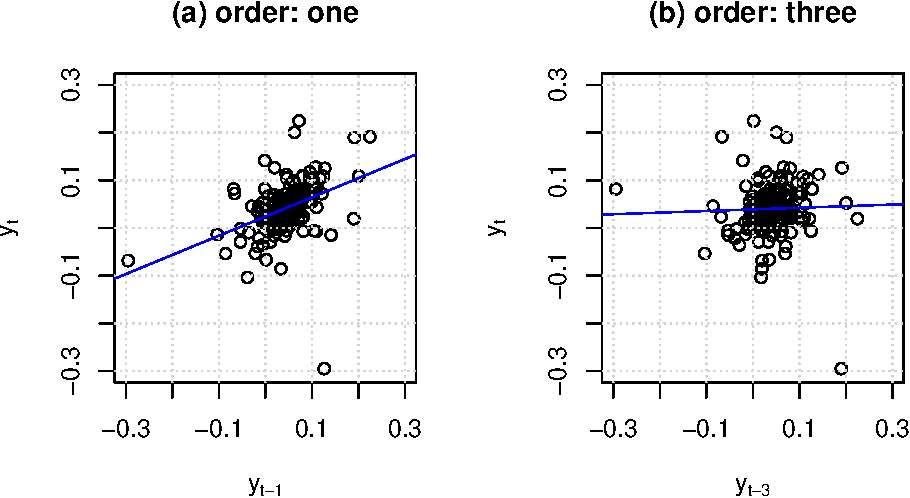
\includegraphics[width=0.95\linewidth]{TimeSeries_files/figure-latex/autocov2-1} \caption{For order $j$, the slope of the blue line is, approximately, $\hat{\gamma}_j/\widehat{\mathbb{V}ar}(y_t)$, where hats indicate sample moments.}\label{fig:autocov2}
\end{figure}

\hypertarget{central-limit-theorem-clt-for-persistent-processes}{%
\section{Central Limit Theorem (CLT) for persistent processes}\label{central-limit-theorem-clt-for-persistent-processes}}

This subsection shows that the Central Limit Theorem (CLT, see Theorem \ref{thm:LindbergLevyCLT}) can be extended to cases where the observations are auto-correlated.

\begin{theorem}[Central Limit Theorem for covariance-stationary processes]
\protect\hypertarget{thm:CLTcovstat}{}\label{thm:CLTcovstat}If process \(y_t\) is covariance stationary and if the series of autocovariances is absolutely summable (\(\sum_{j=-\infty}^{+\infty} |\gamma_j| <\infty\)), then:
\begin{eqnarray}
\bar{y}_T \overset{m.s.}{\rightarrow} \mu &=& \mathbb{E}(y_t) \label{eq:TCL20}\\
\mbox{lim}_{T \rightarrow +\infty} T \mathbb{E}\left[(\bar{y}_T - \mu)^2\right] &=& \sum_{j=-\infty}^{+\infty} \gamma_j \label{eq:TCL2}\\
\sqrt{T}(\bar{y}_T - \mu) &\overset{d}{\rightarrow}& \mathcal{N}\left(0,\sum_{j=-\infty}^{+\infty} \gamma_j \right) \label{eq:TCL4ts}.
\end{eqnarray}

{[}Mean square (m.s.) and distribution (d.) convergences: see Definitions \ref{def:cvgceDistri} and \ref{def:convergenceLr}.{]}
\end{theorem}

\begin{proof}
By Proposition \ref{prp:absMs}, Eq. \eqref{eq:TCL2} implies Eq. \eqref{eq:TCL20}. For Eq. \eqref{eq:TCL2}, see Appendix \ref{AppendixProof}. For Eq. \eqref{eq:TCL4ts}, see \citet{Anderson_1971}, p.~429.
\end{proof}

\begin{definition}[Long-run variance]
\protect\hypertarget{def:LRV}{}\label{def:LRV}Under the assumptions of Theorem \ref{thm:CLTcovstat}, the limit appearing in Eq. \eqref{eq:TCL2} exists and is called \textbf{long-run variance}. It is denoted by \(S\), i.e.:
\[
S = \Sigma_{j=-\infty}^{+\infty} \gamma_j  = \mbox{lim}_{T \rightarrow +\infty} T \mathbb{E}[(\bar{y}_T - \mu)^2].
\]
\end{definition}

If \(y_t\) is ergodic for second moments (see Def. \ref{def:ergod2nd}), a natural estimator of \(S\) is:
\begin{equation}
\hat\gamma_0 + 2 \sum_{\nu=1}^{q} \hat\gamma_\nu, \label{eq:covSmplMean}
\end{equation}
where \(\hat\gamma_\nu = \frac{1}{T}\sum_{\nu+1}^{T} (y_t - \bar{y})(y_{t-\nu} - \bar{y})\).

However, for small samples, Eq. \eqref{eq:covSmplMean} does not necessarily result in a positive definite matrix. \citet{Newey_West_1987} have proposed an estimator that does not have this defect. Their estimator is given by:
\begin{equation}
S^{NW}=\hat\gamma_0 + 2 \sum_{\nu=1}^{q}\left(1-\frac{\nu}{q+1}\right) \hat\gamma_\nu.\label{eq:NWest}
\end{equation}

Loosely speaking, Theorem \ref{thm:CLTcovstat} says that, for a given sample size, the higher the ``persistency'' of a process, the lower the accuracy of the sample mean as an estimate of the population mean. To illustrate, consider three processes that feature the same marginal variance (equal to one, say), but different autocorrelations: 0\%, 70\%, and 99.9\%. Figure \ref{fig:TVTCL} displays simulated paths of such three processes. It indeed appears that, the larger the autocorrelation of the process, the further the sample mean (dashed red line) from the population mean (red solid line).

The same type of simulations can be performed using \href{https://jrenne.shinyapps.io/MacroEc/}{this web interface} (use panel ``AR(1)'').

\begin{figure}
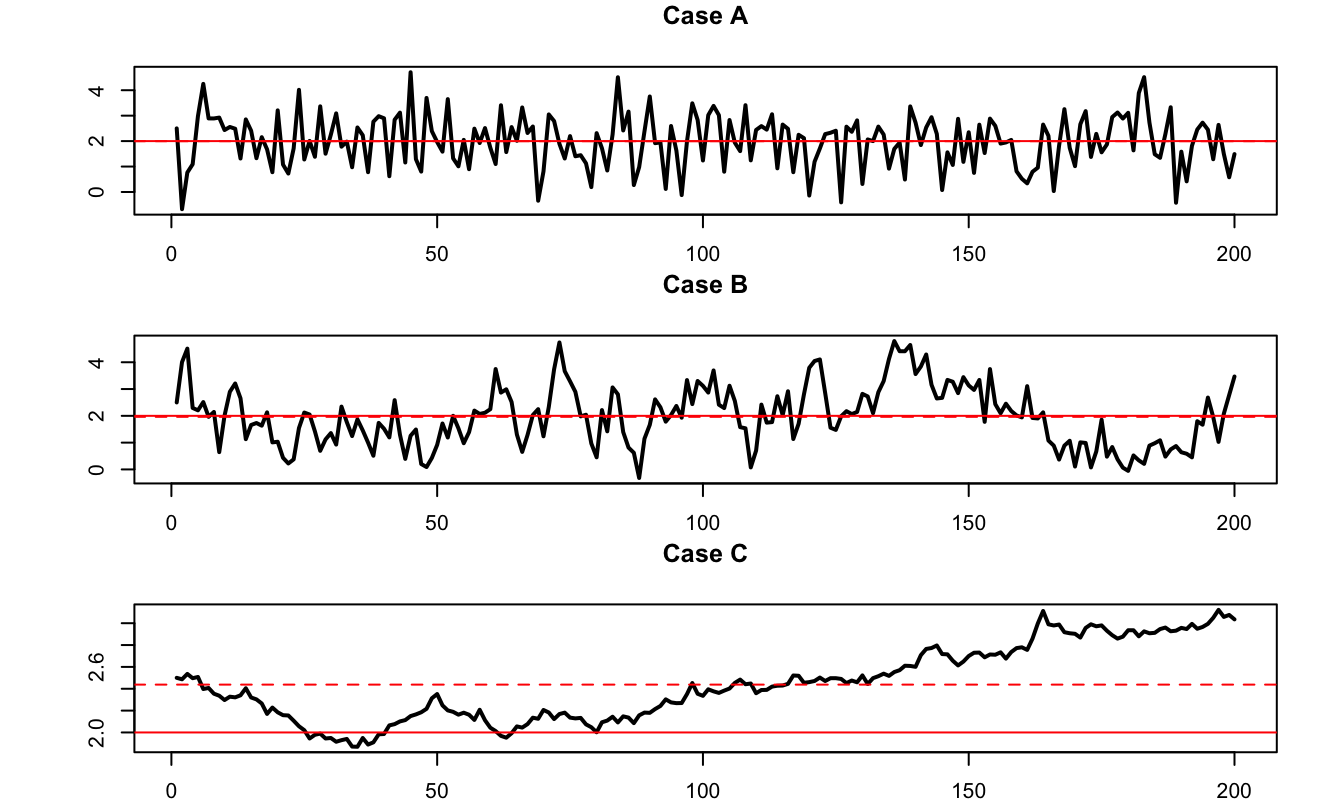
\includegraphics[width=1\linewidth]{TimeSeries_files/figure-latex/TVTCL-1} \caption{The three samples have been simulated using the following data generating process: $x_t = \mu + \rho (x_{t-1}-\mu) + \sqrt{1-\rho^2}\varepsilon_t$, where $\varepsilon_t \sim \mathcal{N}(0,1)$. Case A: $\rho = 0$;  Case B: $\rho = 0.7$;  Case C: $\rho = 0.999$. In the three cases, $\mathbb{E}(x_t)=\mu=2$ and $\mathbb{V}ar(x_t)=1$. The dashed (respectively solid) red line indicate the sample (resp. unconditional) mean.}\label{fig:TVTCL}
\end{figure}

\hypertarget{Univariate}{%
\chapter{Univariate processes}\label{Univariate}}

\hypertarget{moving-average-ma-processes}{%
\section{Moving Average (MA) processes}\label{moving-average-ma-processes}}

Moving average (MA) processes are important basic processes. The moving-average process of order one (MA(1)) is defined as follows:

\begin{definition}[Moving average process of order one]
\protect\hypertarget{def:MA1}{}\label{def:MA1}Process \(y_t\) is a first-order moving average process if, for all \(t\):
\begin{equation}
y_t = \mu + \varepsilon_t + \theta \varepsilon_{t-1},\label{eq:MA1111}
\end{equation}
where \(\{\varepsilon_t\}_{t = -\infty}^{+\infty}\) is a white noise process (see Def. \ref{def:whitenoise}).
\end{definition}

If \(\mathbb{E}(\varepsilon_t^2)=\sigma^2\), it is easily obtained that the unconditional mean and variance of \(y_t\) are:
\[
\mathbb{E}(y_t) = \mu, \quad \mathbb{V}ar(y_t) = (1+\theta^2)\sigma^2.
\]

The first auto-covariance is:
\[
\gamma_1=\mathbb{E}\{(y_t - \mu)(y_{t-1} - \mu)\}=\mathbb{E}\{(\varepsilon_t + \theta \color{red}{\varepsilon_{t-1}})(\color{red}{\varepsilon_{t-1}} + \theta \varepsilon_{t-2})\} = \theta \sigma^2.
\]

It is easily seen that higher-order auto-covariances are zero (\(\gamma_j=0\) for \(j>1\)). Therefore: An MA(1) process is covariance-stationary (Def. \ref{def:covstat}).

From what precedes, the autocorrelation of order \(j\) (see Def. \ref{def:autocor}) of an MA(1) process is given by:
\[
\rho_j =
\left\{
\begin{array}{lll}
1 &\mbox{ if }& j=0,\\
\theta / (1 + \theta^2) &\mbox{ if }& j = 1\\
0 &\mbox{ if }& j>1.
\end{array}
\right.
\]

Notice that process \(y_t\) defined through Eq. \eqref{eq:MA1111}, with \(\mathbb{V}ar(\varepsilon_t)=\sigma^2\), has the same mean and autocovariances as
\[
y_t = \mu + \varepsilon^*_t +\frac{1}{\theta}\varepsilon^*_{t-1},
\]
where \(\mathbb{V}ar(\varepsilon^*_t)=\theta^2\sigma^2\). That is, knowing the mean and auto-covariances of an MA(1) process is not sufficient to identify the process, since two different processes possess the same moments. Only one of these two specifications is said to be \emph{fundamental}, that is the one that satisfies \(|\theta_1|<1\) (see Eq. \eqref{eq:invertible}).

\begin{definition}[MA(q) process]
\protect\hypertarget{def:MAq}{}\label{def:MAq}A \(q^{th}\)-order Moving Average process \(\{y_t\}\) is defined through:
\[
y_t = \mu + \varepsilon_t + \theta_1 \varepsilon_{t-1} + \dots + \theta_q \varepsilon_{t-q},
\]
where \(\{\varepsilon_t\}_{t = -\infty}^{+\infty}\) is a white noise process (Def. \ref{def:whitenoise}).
\end{definition}

\begin{proposition}[Covariance-stationarity of an MA(q) process]
\protect\hypertarget{prp:covMAq}{}\label{prp:covMAq}Finite-order Moving Average processes are covariance-stationary.

Moreover, the autocovariances of an MA(q) process (as defined in Def. \ref{def:MAq}) are given by:
\begin{equation}
\gamma_j = \left\{ \begin{array}{ll} \sigma^2(\theta_j\theta_0 + \theta_{j+1}\theta_{1} +  \dots + \theta_{q}\theta_{q-j}) &\mbox{for} \quad j \in \{0,\dots,q\} \\ 0 &\mbox{for} \quad j>q, \end{array} \right.\label{eq:autocovMA}
\end{equation}
where we use the notation \(\theta_0=1\), and \(\mathbb{V}ar(\varepsilon_t)=\sigma^2\).
\end{proposition}

\begin{proof}
The unconditional expectation of \(y_t\) does not depend on time, since \(\mathbb{E}(y_t)=\mu\). Turning to the autocovariances, we can extend the series of \(\theta_j\)'s by setting \(\theta_j=0\) for \(j>q\). We then have:
\begin{eqnarray*}
\mathbb{E}((y_t-\mu)(y_{t-j}-\mu)) &=& \mathbb{E}\left[(\theta_0 \varepsilon_t +\theta_1 \varepsilon_{t-1} + \dots +\theta_j \color{red}{\varepsilon_{t-j}}+\theta_{j+1} \color{blue}{\varepsilon_{t-j-1}} + \dots) \right.\times \\
&&\left. (\theta_0 \color{red}{\varepsilon_{t-j}} +\theta_1 \color{blue}{\varepsilon_{t-j-1}} + \dots)\right].
\end{eqnarray*}
Using the fact that \(\mathbb{E}(\varepsilon_t\varepsilon_s)=0\) if \(t \ne s\) (because \(\{\varepsilon_t\}_{t = -\infty}^{+\infty}\) is a white noise process) leads to the result.
\end{proof}

Figure \ref{fig:simMA} displays simulated paths of two MA processes (an MA(1) and an MA(4)). Such simulations can also be produced by using panel ``ARMA(p,q)'' of \href{https://jrenne.shinyapps.io/MacroEc/}{this web interface}.

\begin{Shaded}
\begin{Highlighting}[]
\FunctionTok{library}\NormalTok{(AEC)}
\NormalTok{T }\OtherTok{\textless{}{-}} \DecValTok{100}\NormalTok{;nb.sim }\OtherTok{\textless{}{-}} \DecValTok{1}
\NormalTok{y}\FloatTok{.0} \OtherTok{\textless{}{-}} \FunctionTok{c}\NormalTok{(}\DecValTok{0}\NormalTok{)}
\NormalTok{c }\OtherTok{\textless{}{-}} \DecValTok{1}\NormalTok{;phi }\OtherTok{\textless{}{-}} \FunctionTok{c}\NormalTok{(}\DecValTok{0}\NormalTok{);sigma }\OtherTok{\textless{}{-}} \DecValTok{1}
\NormalTok{theta }\OtherTok{\textless{}{-}} \FunctionTok{c}\NormalTok{(}\DecValTok{1}\NormalTok{,}\DecValTok{1}\NormalTok{) }\CommentTok{\# MA(1) specification}
\NormalTok{y.sim }\OtherTok{\textless{}{-}} \FunctionTok{sim.arma}\NormalTok{(c,phi,theta,sigma,T,y}\FloatTok{.0}\NormalTok{,nb.sim)}
\FunctionTok{par}\NormalTok{(}\AttributeTok{mfrow=}\FunctionTok{c}\NormalTok{(}\DecValTok{1}\NormalTok{,}\DecValTok{2}\NormalTok{))}
\FunctionTok{par}\NormalTok{(}\AttributeTok{plt=}\FunctionTok{c}\NormalTok{(.}\DecValTok{2}\NormalTok{,.}\DecValTok{9}\NormalTok{,.}\DecValTok{2}\NormalTok{,.}\DecValTok{85}\NormalTok{))}
\FunctionTok{plot}\NormalTok{(y.sim[,}\DecValTok{1}\NormalTok{],}\AttributeTok{xlab=}\StringTok{""}\NormalTok{,}\AttributeTok{ylab=}\StringTok{""}\NormalTok{,}\AttributeTok{type=}\StringTok{"l"}\NormalTok{,}\AttributeTok{lwd=}\DecValTok{2}\NormalTok{,}
     \AttributeTok{main=}\FunctionTok{expression}\NormalTok{(}\FunctionTok{paste}\NormalTok{(theta[}\DecValTok{0}\NormalTok{],}\StringTok{"=1, "}\NormalTok{,theta[}\DecValTok{1}\NormalTok{],}\StringTok{"=1"}\NormalTok{,}\AttributeTok{sep=}\StringTok{""}\NormalTok{)))}
\FunctionTok{abline}\NormalTok{(}\AttributeTok{h=}\NormalTok{c)}
\NormalTok{theta }\OtherTok{\textless{}{-}} \FunctionTok{c}\NormalTok{(}\DecValTok{1}\NormalTok{,}\DecValTok{1}\NormalTok{,}\DecValTok{1}\NormalTok{,}\DecValTok{1}\NormalTok{,}\DecValTok{1}\NormalTok{) }\CommentTok{\# MA(4) specification}
\NormalTok{y.sim }\OtherTok{\textless{}{-}} \FunctionTok{sim.arma}\NormalTok{(c,phi,theta,sigma,T,y}\FloatTok{.0}\NormalTok{,nb.sim)}
\FunctionTok{plot}\NormalTok{(y.sim[,}\DecValTok{1}\NormalTok{],}\AttributeTok{xlab=}\StringTok{""}\NormalTok{,}\AttributeTok{ylab=}\StringTok{""}\NormalTok{,}\AttributeTok{type=}\StringTok{"l"}\NormalTok{,}\AttributeTok{lwd=}\DecValTok{2}\NormalTok{,}
     \AttributeTok{main=}\FunctionTok{expression}\NormalTok{(}\FunctionTok{paste}\NormalTok{(theta[}\DecValTok{0}\NormalTok{],}\StringTok{"=...="}\NormalTok{,theta[}\DecValTok{4}\NormalTok{],}\StringTok{"=1"}\NormalTok{,}\AttributeTok{sep=}\StringTok{""}\NormalTok{)))}
\FunctionTok{abline}\NormalTok{(}\AttributeTok{h=}\NormalTok{c)}
\end{Highlighting}
\end{Shaded}

\begin{figure}
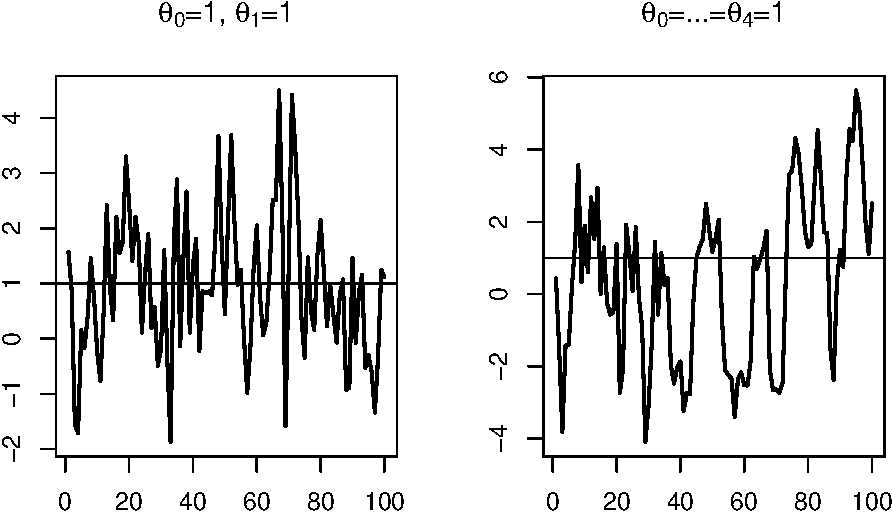
\includegraphics[width=0.95\linewidth]{TimeSeries_files/figure-latex/simMA-1} \caption{Simulation of MA processes.}\label{fig:simMA}
\end{figure}

What if the order \(q\) of an MA(q) process gets infinite? The notion of \textbf{infinite-order Moving Average process} exists and is important in time series analysis, as it relates to impulse response functions (as illustrated in Section \ref{IRFARMA}). The (infinite) sequence of \(\theta_j\) has to satisfy some conditions for such a process to be well-defined (see Theorem \ref{thm:infMA} below). These conditions relate to the ``summability'' of the components of the sequence \(\{\theta_{i}\}_{i\in\mathbb{N}}\):

\begin{definition}[Absolute and square summability]
\protect\hypertarget{def:summability}{}\label{def:summability}The sequence \(\{\theta_{i}\}_{i\in\mathbb{N}}\) is absolutely summable if \(\sum_{i=0}^{\infty}|\theta_i| < + \infty\), and it is square summable if \(\sum_{i=0}^{\infty} \theta_i^2 < + \infty\).
\end{definition}

According to Prop. \ref{prp:absMs} (in the appendix), absolute summability implies square summability.

\begin{theorem}[Existence condition for an infinite MA process]
\protect\hypertarget{thm:infMA}{}\label{thm:infMA}If \(\{\theta_{i}\}_{i\in\mathbb{N}}\) is square summable (see Def. \ref{def:summability}) and if \(\{\varepsilon_t\}_{t = -\infty}^{+\infty}\) is a white noise process (see Def. \ref{def:whitenoise}), then
\[
\mu + \sum_{i=0}^{+\infty} \theta_{i} \varepsilon_{t-i}
\]
defines a well-behaved {[}covariance-stationary{]} process, called infinite-order MA process (MA(\(\infty\))).
\end{theorem}

\begin{proof}
See Appendix 3.A in Hamilton. ``Well behaved'' means that \(\Sigma_{i=0}^{T} \theta_{t-i} \varepsilon_{t-i}\) converges in mean square (Def. \ref{def:convergenceLr}) to some random variable \(Z_t\). The proof makes use of the fact that:
\[
\mathbb{E}\left[\left(\sum_{i=N}^{M}\theta_{i} \varepsilon_{t-i}\right)^2\right] = \sum_{i=N}^{M}|\theta_{i}|^2 \sigma^2,
\]
and that, when \(\{\theta_{i}\}\) is square summable, \(\forall \eta>0\), \(\exists N\) s.t. the right-hand-side term in the last equation is lower than \(\eta\) for all \(M \ge N\) (static Cauchy criterion, Theorem \ref{thm:cauchycritstatic}). This implies that \(\Sigma_{i=0}^{T} \theta_{i} \varepsilon_{t-i}\) converges in mean square (stochastic Cauchy criterion, see Theorem \ref{thm:cauchycritstochastic}).
\end{proof}

\begin{proposition}[First two moments of an infinite MA process]
\protect\hypertarget{prp:momentsMAinf}{}\label{prp:momentsMAinf}

If \(\{\theta_{i}\}_{i\in\mathbb{N}}\) is absolutely summable, i.e., if \(\sum_{i=0}^{\infty}|\theta_i| < + \infty\), then

\begin{enumerate}
\def\labelenumi{\roman{enumi}.}
\tightlist
\item
  \(y_t = \mu + \sum_{i=0}^{+\infty} \theta_{i} \varepsilon_{t-i}\) exists (Theorem \ref{thm:infMA}) and is such that:
  \begin{eqnarray*}
  \mathbb{E}(y_t) &=& \mu\\
  \gamma_0 = \mathbb{E}([y_t-\mu]^2) &=& \sigma^2(\theta_0^2 +\theta_1^2 + \dots)\\
  \gamma_j = \mathbb{E}([y_t-\mu][y_{t-j}-\mu]) &=& \sigma^2(\theta_0\theta_j + \theta_{1}\theta_{j+1} + \dots).
  \end{eqnarray*}
\item
  Process \(y_t\) has absolutely summable auto-covariances, which implies that the results of Theorem \ref{thm:CLTcovstat} (Central Limit) apply.
\end{enumerate}

\end{proposition}

\begin{proof}
The absolute summability of \(\{\theta_{i}\}\) and the fact that \(\mathbb{E}(\varepsilon^2)<\infty\) imply that the order of integration and summation is interchangeable (see Hamilton, 1994, Footnote p.~52), which proves (i). For (ii), see end of Appendix 3.A in Hamilton (1994).
\end{proof}

\hypertarget{ARsection}{%
\section{Auto-Regressive (AR) processes}\label{ARsection}}

\begin{definition}[First-order AR process (AR(1))]
\protect\hypertarget{def:AR1}{}\label{def:AR1}Process \(y_t\) is an AR(1) process if its dynamics is defined by the following difference equation:
\[
y_t = c + \phi y_{t-1} + \varepsilon_t,
\]
where \(\{\varepsilon_t\}_{t = -\infty}^{+\infty}\) is a white noise process (see Def. \ref{def:whitenoise}).
\end{definition}

If \(|\phi|\ge1\), \(y_t\) is not stationary. Indeed, we have:
\begin{eqnarray*}
y_{t+k} &=& c + \varepsilon_{t+k} + \phi  ( c + \varepsilon_{t+k-1})+ \phi^2  ( c + \varepsilon_{t+k-2})+ \dots + \\
&& \phi^{k-1}  ( c + \varepsilon_{t+1}) + \phi^k y_t.
\end{eqnarray*}
Therefore, the conditional variance
\[
\mathbb{V}ar_t(y_{t+k}) = \sigma^2(1 + \phi^2 + \phi^4 + \dots + \phi^{2(k-1)})
\]
(where \(\sigma^2\) is the variance of \(\varepsilon_t\)) does not converge when \(k\) gets infinitely large. This implies that \(\mathbb{V}ar(y_{t})\) does not exist.\footnote{Indeed, by the law of total variance \(\mathbb{V}ar(y_{t})=\mathbb{V}ar(\mathbb{E}_{t-k}(y_{t}))+\mathbb{E}(\mathbb{V}ar_{t-k}(y_{t}))>\). Since we have \(\mathbb{V}ar(\mathbb{E}_{t-k}(y_{t})) \ge 0\) and \(\mathbb{E}(\mathbb{V}ar_{t-k}(y_{t}))=\mathbb{V}ar_{t-k}(y_{t})\) that goes to \(+\infty\) (by what precedes), it comes that \(\mathbb{V}ar(y_{t})\) is not finite.} By contrast, if \(|\phi| < 1\), we have:
\[
y_t = c + \varepsilon_t + \phi  ( c + \varepsilon_{t-1})+ \phi^2  ( c + \varepsilon_{t-2})+ \dots + \phi^k  ( c + \varepsilon_{t-k}) + \dots
\]
Hence, if \(|\phi| < 1\), the unconditional mean and variance of \(y_t\) are:
\[
\mathbb{E}(y_t) = \frac{c}{1-\phi} =: \mu \quad \mbox{and} \quad \mathbb{V}ar(y_t) = \frac{\sigma^2}{1-\phi^2}.
\]

Let us compute the \(j^{th}\) autocovariance of the AR(1) process:
\begin{eqnarray*}
\mathbb{E}([y_{t} - \mu][y_{t-j} - \mu]) &=& \mathbb{E}([\varepsilon_t + \phi  \varepsilon_{t-1}+ \phi^2 \varepsilon_{t-2} + \dots + \color{red}{\phi^j \varepsilon_{t-j}} + \color{blue}{\phi^{j+1} \varepsilon_{t-j-1}} \dots]\times \\
&&[\color{red}{\varepsilon_{t-j}} + \color{blue}{\phi \varepsilon_{t-j-1}} + \phi^2 \varepsilon_{t-j-2} + \dots + \phi^k \varepsilon_{t-j-k} + \dots])\\
&=& \mathbb{E}(\color{red}{\phi^j \varepsilon_{t-j}^2}+\color{blue}{\phi^{j+2} \varepsilon_{t-j-1}^2}+\phi^{j+4} \varepsilon_{t-j-2}^2+\dots)\\
&=& \frac{\phi^j \sigma^2}{1 - \phi^2}.
\end{eqnarray*}

Therefore, the auto-correlation is given by \(\rho_j = \phi^j\).

By what precedes, we have:

\begin{proposition}[Covariance-stationarity of an AR(1) process]
\protect\hypertarget{prp:statioAR1}{}\label{prp:statioAR1}The AR(1) process, as defined in Def. \ref{def:AR1}, is covariance-stationary iff \(|\phi|<1\).
\end{proposition}

\begin{definition}[AR(p) process]
\protect\hypertarget{def:ARp}{}\label{def:ARp}Process \(y_t\) is a \(p^{th}\)-order autoregressive process (AR(p)) if its dynamics is defined by the following difference equation (with \(\phi_p \ne 0\)):
\begin{equation}
y_t = c + \phi_1 y_{t-1} + \phi_2 y_{t-2} + \dots + \phi_p y_{t-p} + \varepsilon_t,\label{eq:AR}
\end{equation}
where \(\{\varepsilon_t\}_{t = -\infty}^{+\infty}\) is a white noise process (see Def. \ref{def:whitenoise}).
\end{definition}

As we will see, the covariance-stationarity of process \(y_t\) hinges on the eigenvalues of matrix \(F\), defined as:
\begin{equation}
F = \left[
\begin{array}{ccccc}
\phi_1 & \phi_2 & \dots& & \phi_p \\
1 & 0 &\dots && 0 \\
0 & 1 &\dots && 0 \\
\vdots &  & \ddots && \vdots \\
0 & 0 &\dots &1& 0 \\
\end{array}
\right].\label{eq:F}
\end{equation}

Note that this matrix \(F\) is such that if \(y_t\) follows Eq. \eqref{eq:AR}, then process \(\mathbf{y}_t\) follows:
\[
\mathbf{y}_t = \mathbf{c} + F \mathbf{y}_{t-1} + \boldsymbol\xi_t
\]
with
\[
\mathbf{c} =
\left[\begin{array}{c}
c\\
0\\
\vdots\\
0
\end{array}\right],
\quad
\boldsymbol\xi_t =
\left[\begin{array}{c}
\varepsilon_t\\
0\\
\vdots\\
0
\end{array}\right],
\quad
\mathbf{y}_t =
\left[\begin{array}{c}
y_t\\
y_{t-1}\\
\vdots\\
y_{t-p+1}
\end{array}\right].
\]

\begin{proposition}[The eigenvalues of matrix F]
\protect\hypertarget{prp:Feigen}{}\label{prp:Feigen}The eigenvalues of \(F\) (defined by Eq. \eqref{eq:F}) are the solutions of:
\begin{equation}
\lambda^p - \phi_1 \lambda^{p-1} - \dots - \phi_{p-1}\lambda - \phi_p = 0.\label{eq:Feigen}
\end{equation}
\end{proposition}

\begin{proposition}[Covariance-stationarity of an AR(p) process]
\protect\hypertarget{prp:stability}{}\label{prp:stability}

These four statements are equivalent:

\begin{enumerate}
\def\labelenumi{\roman{enumi}.}
\tightlist
\item
  Process \(\{y_t\}\), defined in Def. \ref{def:ARp}, is covariance-stationary.
\item
  The eigenvalues of \(F\) (as defined Eq. \eqref{eq:F}) lie strictly within the unit circle.
\item
  The roots of Eq. \eqref{eq:outside} (below) lie strictly outside the unit circle.
  \begin{equation}
  1 - \phi_1 z - \dots - \phi_{p-1}z^{p-1} - \phi_p z^p = 0.\label{eq:outside}
  \end{equation}
\item
  The roots of Eq. \eqref{eq:inside} (below) lie strictly inside the unit circle.
  \begin{equation}
  \lambda^p - \phi_1 \lambda^{p-1} - \dots - \phi_{p-1}\lambda - \phi_p = 0.\label{eq:inside}
  \end{equation}
\end{enumerate}

\end{proposition}

\begin{proof}
We consider the case where the eigenvalues of \(F\) are distinct.\footnote{The Jordan matrix decomposition can be used in the general case.} When the eigenvalues of \(F\) are distinct, \(F\) admits the following spectral decomposition: \(F = PDP^{-1}\), where \(D\) is diagonal. Using the notations introduced in Eq. \eqref{eq:F}, we have:
\[
\mathbf{y}_{t} = \mathbf{c} + F \mathbf{y}_{t-1} + \boldsymbol\xi_{t}.
\]
Let's introduce \(\mathbf{d} = P^{-1}\mathbf{c}\), \(\mathbf{z}_t = P^{-1}\mathbf{y}_t\) and \(\boldsymbol\eta_t = P^{-1}\boldsymbol\xi_t\). We have:
\[
\mathbf{z}_{t} = \mathbf{d} + D \mathbf{z}_{t-1} + \boldsymbol\eta_{t}.
\]
Because \(D\) is diagonal, the different component of \(\mathbf{z}_t\), denoted by \(z_{i,t}\), follow AR(1) processes. The (scalar) autoregressive parameters of these AR(1) processes are the diagonal entries of \(D\)---which also are the eigenvalues of \(F\)---that we denote by \(\lambda_i\).

Process \(y_t\) is covariance-stationary iff \(\mathbf{y}_{t}\) also is covariance-stationary, which is the case iff all \(z_{i,t}\), \(i \in \{1,\dots,p\}\), are covariance-stationary. By Prop. \ref{prp:statioAR1}, process \(z_{i,t}\) is covariance-stationary iff \(|\lambda_i|<1\). This proves that (i) is equivalent to (ii). Prop. \ref{prp:Feigen} further proves that (ii) is equivalent to (iv). Finally, it is easily seen that (iii) is equivalent to (iv) (as long as \(\phi_p \ne 0\)).
\end{proof}

Using the lag operator (see Eq \eqref{eq:lagOp}), if \(y_t\) is a covariance-stationary AR(p) process (Def. \ref{def:ARp}), we can write:
\[
y_t = \mu + \psi(L)\varepsilon_t,
\]
where
\begin{equation}
\psi(L) = (1 - \phi_1 L - \dots - \phi_p L^p)^{-1},
\end{equation}
and
\begin{equation}
\mu = \mathbb{E}(y_t) = \dfrac{c}{1-\phi_1 -\dots - \phi_p}.\label{eq:EAR}
\end{equation}

In the following lines of codes, we compute the eigenvalues of the \(F\) matrices associated with the following processes (where \(\varepsilon_t\) is a white noise):
\begin{eqnarray*}
x_t &=& 0.9 x_{t-1} -0.2 x_{t-2} + \varepsilon_t\\
y_t &=& 1.1 y_{t-1} -0.3 y_{t-2} + \varepsilon_t\\
w_t &=& 1.4 w_{t-1} -0.7 w_{t-2} + \varepsilon_t\\
z_t &=& 0.9 z_{t-1} +0.2 z_{t-2} + \varepsilon_t.
\end{eqnarray*}

\begin{Shaded}
\begin{Highlighting}[]
\NormalTok{F }\OtherTok{\textless{}{-}} \FunctionTok{matrix}\NormalTok{(}\FunctionTok{c}\NormalTok{(.}\DecValTok{9}\NormalTok{,}\DecValTok{1}\NormalTok{,}\SpecialCharTok{{-}}\NormalTok{.}\DecValTok{2}\NormalTok{,}\DecValTok{0}\NormalTok{),}\DecValTok{2}\NormalTok{,}\DecValTok{2}\NormalTok{)}
\NormalTok{lambda\_x }\OtherTok{\textless{}{-}} \FunctionTok{eigen}\NormalTok{(F)}\SpecialCharTok{$}\NormalTok{values}
\NormalTok{F[}\DecValTok{1}\NormalTok{,] }\OtherTok{\textless{}{-}} \FunctionTok{c}\NormalTok{(}\FloatTok{1.1}\NormalTok{,}\SpecialCharTok{{-}}\NormalTok{.}\DecValTok{3}\NormalTok{)}
\NormalTok{lambda\_y }\OtherTok{\textless{}{-}} \FunctionTok{eigen}\NormalTok{(F)}\SpecialCharTok{$}\NormalTok{values}
\NormalTok{F[}\DecValTok{1}\NormalTok{,] }\OtherTok{\textless{}{-}} \FunctionTok{c}\NormalTok{(}\FloatTok{1.4}\NormalTok{,}\SpecialCharTok{{-}}\NormalTok{.}\DecValTok{7}\NormalTok{)}
\NormalTok{lambda\_w }\OtherTok{\textless{}{-}} \FunctionTok{eigen}\NormalTok{(F)}\SpecialCharTok{$}\NormalTok{values}
\NormalTok{F[}\DecValTok{1}\NormalTok{,] }\OtherTok{\textless{}{-}} \FunctionTok{c}\NormalTok{(.}\DecValTok{9}\NormalTok{,.}\DecValTok{2}\NormalTok{)}
\NormalTok{lambda\_z }\OtherTok{\textless{}{-}} \FunctionTok{eigen}\NormalTok{(F)}\SpecialCharTok{$}\NormalTok{values}
\FunctionTok{rbind}\NormalTok{(lambda\_x,lambda\_y,lambda\_w,lambda\_z)}
\end{Highlighting}
\end{Shaded}

\begin{verbatim}
##                         [,1]                  [,2]
## lambda_x 0.500000+0.0000000i  0.4000000+0.0000000i
## lambda_y 0.600000+0.0000000i  0.5000000+0.0000000i
## lambda_w 0.700000+0.4582576i  0.7000000-0.4582576i
## lambda_z 1.084429+0.0000000i -0.1844289+0.0000000i
\end{verbatim}

The absolute values of the eigenvalues associated with process \(w_t\) are both equal to 0.837. Therefore, according to Proposition \ref{prp:stability}, processes \(x_t\), \(y_t\), and \(w_t\) are covariance-stationary, but not \(z_t\) (because, for the latter process, the absolute value of one of the eigenvalues of matrix \(F\) is larger than 1).

The computation of the autocovariances of \(y_t\) is based on the so-called \textbf{Yule-Walker equations} (Eq. \eqref{eq:gammas}). Let's rewrite Eq. \eqref{eq:AR}:
\[
(y_t-\mu) = \phi_1 (y_{t-1}-\mu) + \phi_2 (y_{t-2}-\mu) + \dots + \phi_p (y_{t-p}-\mu) + \varepsilon_t.
\]
Multiplying both sides by \(y_{t-j}-\mu\) and taking expectations leads to the (Yule-Walker) equations:
\begin{equation}
\gamma_j = \left\{
\begin{array}{l}
\phi_1 \gamma_{j-1}+\phi_2 \gamma_{j-2}+ \dots + \phi_p \gamma_{j-p} \quad if \quad j>0\\
\phi_1 \gamma_{1}+\phi_2 \gamma_{2}+ \dots + \phi_p \gamma_{p} + \sigma^2 \quad for \quad j=0,
\end{array}
\right.\label{eq:gammas}
\end{equation}
where \(\sigma^2\) is the variance of \(\varepsilon_t\).

Using \(\gamma_j = \gamma_{-j}\) (Prop. \ref{prp:gammaMinus}), one can express \((\gamma_0,\gamma_1,\dots,\gamma_{p})\) as functions of \((\sigma^2,\phi_1,\dots,\phi_p)\). Indeed, we have:
\[
\left[\begin{array}{c}
\gamma_0 \\
\gamma_1 \\
\gamma_2 \\
\vdots\\
\gamma_p
\end{array}\right] =
\underbrace{\left[\begin{array}{cccccccc}
0 & \phi_1 & \phi_2 & \dots &&& \phi_p \\
\phi_1 & \phi_2 & \dots &&& \phi_p & 0 \\
\phi_2 & (\phi_1 + \phi_3) & \phi_4 & \dots & \phi_p& 0& 0 \\
\vdots\\
\phi_p & \phi_{p-1} & \dots &&\phi_2& \phi_1 & 0
\end{array}\right]}_{=H}\left[\begin{array}{c}
\gamma_0 \\
\gamma_1 \\
\gamma_2 \\
\vdots\\
\gamma_p
\end{array}\right] +
\left[\begin{array}{c}
\sigma^2 \\
0 \\
0 \\
\vdots\\
0
\end{array}\right],
\]

which is easily solved by inversing matrix \(H\).

\hypertarget{ar-ma-processes}{%
\section{AR-MA processes}\label{ar-ma-processes}}

\begin{definition}[ARMA(p,q) process]
\protect\hypertarget{def:ARMApq}{}\label{def:ARMApq}\(\{y_t\}\) is an ARMA(\(p\),\(q\)) process if its dynamics is described by the following equation:
\begin{equation}
y_t = c + \underbrace{\phi_1 y_{t-1} + \dots + \phi_p y_{t-p}}_{\mbox{AR part}} + \underbrace{\varepsilon_t + \theta_1 \varepsilon_{t-1} + \dots + \theta_q \varepsilon_{t-q}}_{\mbox{MA part}},\label{eq:ARMApq}
\end{equation}
where \(\{\varepsilon_t\}_{t \in ] -\infty,+\infty[}\), of variance \(\sigma^2\) (say), is a white noise process (see Def. \ref{def:whitenoise}).
\end{definition}

\begin{proposition}[Stationarity of an ARMA(p,q) process]
\protect\hypertarget{prp:statioARMApq}{}\label{prp:statioARMApq}The ARMA(\(p\),\(q\)) process defined in \ref{def:ARMApq} is covariance stationary iff the roots of
\[
1 - \phi_1 z - \dots - \phi_p z^p=0
\]
lie strictly outside the unit circle or, equivalently, iff those of
\[
\lambda^p - \phi_1 \lambda^{p-1} - \dots - \phi_p=0
\]
lie strictly within the unit circle.
\end{proposition}

\begin{proof}
The proof of Prop. \ref{prp:stability} can be adapted to the present case.
\end{proof}

We can write:
\[
(1 - \phi_1 L - \dots - \phi_p L^p)y_t = c + (1 + \theta_1 L + \dots + \theta_q L^q)\varepsilon_t.
\]

If the roots of \(1 - \phi_1 z - \dots - \phi_p z^p=0\) lie outside the unit circle, we have:
\begin{equation}
y_t = \mu + \psi(L)\varepsilon_t,\label{eq:ARMAwold}
\end{equation}
where
\[
\psi(L) = \frac{1 + \theta_1 L + \dots + \theta_q L^q}{1 - \phi_1 L - \dots - \phi_p L^p} \quad and \quad \mu = \dfrac{c}{1-\phi_1 -\dots - \phi_p}.
\]

Eq. \eqref{eq:ARMAwold} is the \textbf{Wold representation} of this ARMA process (see Theorem \ref{thm:Wold} below). In Section \ref{IRFARMA} (and more precisely in Proposition \ref{prp:computPsi}), we will see how to obtain the first \(h\) terms of the infinite polynomial \(\Psi(L)\).

Importantly, note that the stationarity of the process depends only on the AR specification (or on the eigenvalues of matrix \(F\), exactly as in Prop. \ref{prp:stability}). When an ARMA process is stationary, the weights in \(\psi(L)\) decay at a geometric rate.

\hypertarget{PACFapproach}{%
\section{PACF approach to identify AR/MA processes}\label{PACFapproach}}

We have seen that the \(k^{th}\)-order auto-correlation of an MA(q) process is null if \(k>q\). This is exploited, in practice, to determine the order of an MA process. Moreover, since this is not the case for an AR process, this can be used to distinguish an AR from an MA process.

There exists an equivalent condition that satisfied by AR processes, and that can be used to determine whether a process can be modeled as such a process. This condition relates to partial auto-correlations:

\begin{definition}[Partial auto-correlation]
\protect\hypertarget{def:partialAC}{}\label{def:partialAC}The partial auto-correlation (\(\phi_{h,h}\)) of process \(\{y_t\}\) is defined as the partial correlation of \(y_{t+h}\) and \(y_t\) given \(y_{t+h-1},\dots,y_{t+1}\). (see Def. \ref{def:partialcorrel} for the definition of partial correlation.)
\end{definition}

If \(h>p\), the regression of \(y_{t+h}\) on \(y_{t+h-1},\dots,y_{t+1}\) is:
\[
y_{t+h} = c + \phi_1 y_{t+h-1}+\dots+ \phi_p  y_{t+h-p} + \varepsilon_{t+h}.
\]
The residuals of the latter regressions (\(\varepsilon_{t+h}\)) are uncorrelated to \(y_t\). Then the partial autocorrelation is zero for \(h>p\).

Besides, it can be shown that \(\phi_{p,p}=\phi_p\). Hence \(\phi_{p,p}=\phi_p\) but \(\phi_{h,h}=0\) for \(h>p\). This can be used to determine the order of an AR process. By contrast (importantly) if \(y_t\) follows an MA(q) process, then \(\phi_{k,k}\) asymptotically approaches zero instead of cutting off abruptly.

As illustrated below, the functions \texttt{acf} and \texttt{pacf} of R allow to conveniently implement the (P)ACF approach. (In these lines of codes, note also the use of function \texttt{sim.arma} to simulate ARMA processes.)

\begin{Shaded}
\begin{Highlighting}[]
\FunctionTok{library}\NormalTok{(AEC)}
\FunctionTok{par}\NormalTok{(}\AttributeTok{mfrow=}\FunctionTok{c}\NormalTok{(}\DecValTok{3}\NormalTok{,}\DecValTok{2}\NormalTok{))}
\FunctionTok{par}\NormalTok{(}\AttributeTok{plt=}\FunctionTok{c}\NormalTok{(.}\DecValTok{2}\NormalTok{,.}\DecValTok{9}\NormalTok{,.}\DecValTok{2}\NormalTok{,.}\DecValTok{95}\NormalTok{))}
\NormalTok{theta }\OtherTok{\textless{}{-}} \FunctionTok{c}\NormalTok{(}\DecValTok{1}\NormalTok{,}\DecValTok{2}\NormalTok{,}\DecValTok{1}\NormalTok{);phi}\OtherTok{=}\DecValTok{0}
\NormalTok{y.sim }\OtherTok{\textless{}{-}} \FunctionTok{sim.arma}\NormalTok{(}\AttributeTok{c=}\DecValTok{0}\NormalTok{,phi,theta,}\AttributeTok{sigma=}\DecValTok{1}\NormalTok{,}\AttributeTok{T=}\DecValTok{1000}\NormalTok{,}\AttributeTok{y.0=}\DecValTok{0}\NormalTok{,}\AttributeTok{nb.sim=}\DecValTok{1}\NormalTok{)}
\FunctionTok{par}\NormalTok{(}\AttributeTok{mfg=}\FunctionTok{c}\NormalTok{(}\DecValTok{1}\NormalTok{,}\DecValTok{1}\NormalTok{));}\FunctionTok{plot}\NormalTok{(y.sim,}\AttributeTok{type=}\StringTok{"l"}\NormalTok{,}\AttributeTok{lwd=}\DecValTok{2}\NormalTok{)}
\FunctionTok{par}\NormalTok{(}\AttributeTok{mfg=}\FunctionTok{c}\NormalTok{(}\DecValTok{2}\NormalTok{,}\DecValTok{1}\NormalTok{));}\FunctionTok{acf}\NormalTok{(y.sim)}
\FunctionTok{par}\NormalTok{(}\AttributeTok{mfg=}\FunctionTok{c}\NormalTok{(}\DecValTok{3}\NormalTok{,}\DecValTok{1}\NormalTok{));}\FunctionTok{pacf}\NormalTok{(y.sim)}
\NormalTok{theta }\OtherTok{\textless{}{-}} \FunctionTok{c}\NormalTok{(}\DecValTok{1}\NormalTok{);phi}\OtherTok{=}\FloatTok{0.9}
\NormalTok{y.sim }\OtherTok{\textless{}{-}} \FunctionTok{sim.arma}\NormalTok{(}\AttributeTok{c=}\DecValTok{0}\NormalTok{,phi,theta,}\AttributeTok{sigma=}\DecValTok{1}\NormalTok{,}\AttributeTok{T=}\DecValTok{1000}\NormalTok{,}\AttributeTok{y.0=}\DecValTok{0}\NormalTok{,}\AttributeTok{nb.sim=}\DecValTok{1}\NormalTok{)}
\FunctionTok{par}\NormalTok{(}\AttributeTok{mfg=}\FunctionTok{c}\NormalTok{(}\DecValTok{1}\NormalTok{,}\DecValTok{2}\NormalTok{));}\FunctionTok{plot}\NormalTok{(y.sim,}\AttributeTok{type=}\StringTok{"l"}\NormalTok{,}\AttributeTok{lwd=}\DecValTok{2}\NormalTok{)}
\FunctionTok{par}\NormalTok{(}\AttributeTok{mfg=}\FunctionTok{c}\NormalTok{(}\DecValTok{2}\NormalTok{,}\DecValTok{2}\NormalTok{));}\FunctionTok{acf}\NormalTok{(y.sim)}
\FunctionTok{par}\NormalTok{(}\AttributeTok{mfg=}\FunctionTok{c}\NormalTok{(}\DecValTok{3}\NormalTok{,}\DecValTok{2}\NormalTok{));}\FunctionTok{pacf}\NormalTok{(y.sim)}
\end{Highlighting}
\end{Shaded}

\begin{figure}
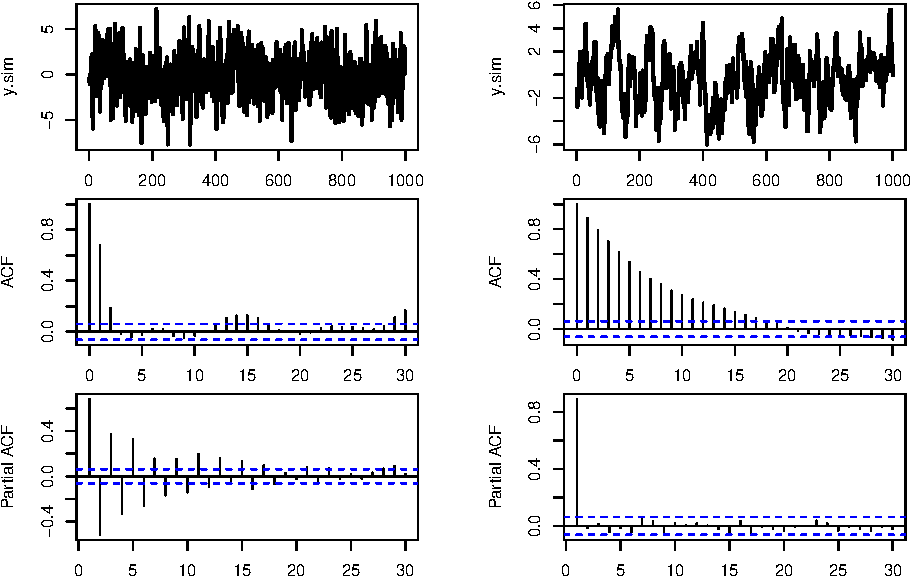
\includegraphics[width=1\linewidth]{TimeSeries_files/figure-latex/pacf-1} \caption{ACF/PACF analysis of two processes (MA process on the left, AR on the right). The correlations are computed on samples of length 1000.}\label{fig:pacf}
\end{figure}

\hypertarget{wold-decomposition}{%
\section{Wold decomposition}\label{wold-decomposition}}

The Wold decomposition is an important result in time series analysis:

\begin{theorem}[Wold decomposition]
\protect\hypertarget{thm:Wold}{}\label{thm:Wold}

Any covariance-stationary process admits the following representation:
\[
y_t = \mu + \sum_{0}^{+\infty} \theta_i \varepsilon_{t-i} + \kappa_t,
\]
where

\begin{itemize}
\tightlist
\item
  \(\theta_0 = 1\), \(\sum_{i=0}^{\infty} \theta_i^2 < +\infty\) (square summability, see Def. \ref{def:summability}).
\item
  \(\{\varepsilon_t\}\) is a white noise (see Def. \ref{def:whitenoise}); \(\varepsilon_t\) is the error made when forecasting \(y_t\) based on a linear combination of lagged \(y_t\)'s (\(\varepsilon_t = y_t - \hat{\mathbb{E}}[y_t|y_{t-1},y_{t-2},\dots]\)).
\item
  For any \(j \ge 1\), \(\kappa_t\) is not correlated with \(\varepsilon_{t-j}\); but \(\kappa_t\) can be perfectly forecasted based on a linear combination of lagged \(y_t\)'s (i.e.~\(\kappa_t = \hat{\mathbb{E}}(\kappa_t|y_{t-1},y_{t-2},\dots)\)). \(\kappa_t\) is called the \textbf{deterministic component} of \(y_t\).
\end{itemize}

\end{theorem}

\begin{proof}
See \citet{Anderson_1971}. Partial proof in \href{http://faculty.wcas.northwestern.edu/~lchrist/finc520/wold.pdf}{L. Christiano}'s lecture notes.
\end{proof}

For an ARMA process, the Wold representation is given by Eq. \eqref{eq:ARMAwold}. As detailed in Prop. \ref{prp:computPsi}, it can be computed by recursively replacing the lagged \(y_t\)'s in Eq. \eqref{eq:ARMApq}. In this case, the deterministic component (\(\kappa\)) is null.

\hypertarget{IRFARMA}{%
\section{Impulse Response Functions (IRFs) in ARMA models}\label{IRFARMA}}

Consider the ARMA(p,q) process defined in Def. \ref{def:ARMApq}. Let us construct a novel (counterfactual) sequence of shocks \(\{\tilde\varepsilon_t^{(s)}\}\):
\[
\tilde\varepsilon_t^{(s)} = \left\{
\begin{array}{lcc}
\varepsilon_{t} & if & t \ne s,\\
\varepsilon_{t} + 1 &if& t=s.
\end{array}
\right.
\]
Hence, the only difference between processes \(\{\varepsilon_t^{(s)}\}\) and \(\{\tilde\varepsilon_t^{(s)}\}\) pertains to date \(s\), where \(\varepsilon_s\) is replaced with \(\varepsilon_s + 1\) in \(\{\tilde\varepsilon_t^{(s)}\}\).

We denote by \(\{\tilde{y}_t^{(s)}\}\) the process following Eq. \eqref{eq:ARMApq} where \(\{\varepsilon_t\}\) is replaced with \(\{\tilde\varepsilon_t^{(s)}\}\). The time series \(\{\tilde{y}_t^{(s)}\}\) is the counterfactual series \(\{y_t\}\) that would have prevailed if \(\varepsilon_t\) had been shifted by one unit on date \(s\) (and that would be the only change).

The relationship between \(\{y_t\}\) and \(\{\tilde{y}_t^{(s)}\}\) defines the \textbf{dynamic multipliers} of \(\{y_t\}\). The dynamic multiplier \(\frac{\partial y_t}{\partial \varepsilon_{s}}\) corresponds to the impact on \(y_t\) of a unit increase in \(\varepsilon_s\) (on date \(s\)). Using the notation introduced before for \(\tilde{y}_t^{(s)}\), we have:
\[
\tilde{y}_t^{(s)} = y_t + \frac{\partial y_t}{\partial \varepsilon_{s}}.
\]
Let us show that the dynamic multipliers are closely related to the infinite MA representation (or \textbf{Wold decomposition}, Theorem \ref{thm:Wold}) of \(y_t\):
\[
y_t = \mu + \sum_{i=0}^{+\infty} \psi_i \varepsilon_{t-i}.
\]
For \(t<s\), we have \(y_t = \tilde{y}_t^{(s)}\) (because \(\tilde{\varepsilon}_{t-i}= \varepsilon_{t-i}\) for all \(i \ge 0\) if \(t<s\)).

For \(t \ge s\):
\[
\tilde{y}_t^{(s)} = \mu + \left( \sum_{i=0}^{t-s-1} \psi_i \varepsilon_{t-i} \right) + \psi_{t-s}(\varepsilon_{s}+1) + \left( \sum_{i=t-s+1}^{+\infty} \psi_i \varepsilon_{t-i} \right)=y_t + \frac{\partial y_t}{\partial \varepsilon_{s}}.
\]
Therefore, it comes that the only difference between \(\tilde{y}_t^{(s)}\) and \(y_t\) is \(\psi_{t-s}\). As a result, for \(t \ge s\), we have:
\[
\boxed{\dfrac{\partial y_t}{\partial \varepsilon_{s}}=\psi_{t-s}.}
\]
That is, \(\{y_t\}\)'s dynamic multiplier of order \(k\) is the same object as the \(k^{th}\) loading \(\psi_k\) in the Wold decomposition of \(\{y_t\}\). The sequence \(\left\{\dfrac{\partial y_{t+h}}{\partial \varepsilon_{t}}\right\}_{h \ge 0} \equiv \left\{\psi_h\right\}_{h \ge 0}\) defines the \textbf{impulse response function (IRF)} of \(y_t\) to the shock \(\varepsilon_t\).

For ARMA processes, one can compute the IRFs (or the Wold decomposition) by using a simple recursive algorithm:

\begin{proposition}[IRF of an ARMA(p,q) process]
\protect\hypertarget{prp:computPsi}{}\label{prp:computPsi}

The coefficients \(\psi_h\), that define the IRF of process \(y_t\) to \(\varepsilon_t\), can be computed recursively as follows:

\begin{enumerate}
\def\labelenumi{\arabic{enumi}.}
\tightlist
\item
  Set \(\psi_{-1}=\dots=\psi_{-p}=0\).
\item
  For \(h \ge 0\), (recursively) apply:
  \[
  \psi_h = \phi_1 \psi_{h-1} + \dots + \phi_p \psi_{h-p} + \theta_h,
  \]
  where \(\theta_h = 0\) for \(h>q\).
\end{enumerate}

\end{proposition}

\begin{proof}
This is obtained by applying the operator \(\frac{\partial}{\partial \varepsilon_{t}}\) on both sides of Eq. \eqref{eq:ARMApq}:
\[
y_{t+h} = c + \phi_1 y_{t+h-1} + \dots + \phi_p y_{t+h-p} + \varepsilon_{t+h} + \theta_1 \varepsilon_{t+h-1} + \dots + \theta_q \varepsilon_{t+h-q}.
\]
\end{proof}

Note that Proposition \ref{prp:computPsi} constitutes a simple way to compute the MA(\(\infty\)) representation (or Wold representation) of an ARMA process.

One can use function \texttt{sim.arma} of package \texttt{AEC} to compute ARMA's IRFs (with the argument \texttt{make.IRF\ =\ 1}):

\begin{Shaded}
\begin{Highlighting}[]
\NormalTok{T }\OtherTok{\textless{}{-}} \DecValTok{21} \CommentTok{\# number of periods for IRF}
\NormalTok{theta }\OtherTok{\textless{}{-}} \FunctionTok{c}\NormalTok{(}\DecValTok{1}\NormalTok{,}\DecValTok{1}\NormalTok{,}\DecValTok{1}\NormalTok{);phi }\OtherTok{\textless{}{-}} \FunctionTok{c}\NormalTok{(}\DecValTok{0}\NormalTok{);c }\OtherTok{\textless{}{-}} \DecValTok{0}
\NormalTok{y.sim }\OtherTok{\textless{}{-}} \FunctionTok{sim.arma}\NormalTok{(c,phi,theta,}\AttributeTok{sigma=}\DecValTok{1}\NormalTok{,T,}\AttributeTok{y.0=}\FunctionTok{rep}\NormalTok{(}\DecValTok{0}\NormalTok{,}\FunctionTok{length}\NormalTok{(phi)),}
                  \AttributeTok{nb.sim=}\DecValTok{1}\NormalTok{,}\AttributeTok{make.IRF =} \DecValTok{1}\NormalTok{)}
\FunctionTok{par}\NormalTok{(}\AttributeTok{mfrow=}\FunctionTok{c}\NormalTok{(}\DecValTok{1}\NormalTok{,}\DecValTok{3}\NormalTok{));}\FunctionTok{par}\NormalTok{(}\AttributeTok{plt=}\FunctionTok{c}\NormalTok{(.}\DecValTok{25}\NormalTok{,.}\DecValTok{95}\NormalTok{,.}\DecValTok{2}\NormalTok{,.}\DecValTok{85}\NormalTok{))}
\FunctionTok{plot}\NormalTok{(}\DecValTok{0}\SpecialCharTok{:}\NormalTok{(T}\DecValTok{{-}1}\NormalTok{),y.sim[,}\DecValTok{1}\NormalTok{],}\AttributeTok{type=}\StringTok{"l"}\NormalTok{,}\AttributeTok{lwd=}\DecValTok{2}\NormalTok{,}
     \AttributeTok{main=}\StringTok{"(a) Process 1"}\NormalTok{,}\AttributeTok{xlab=}\StringTok{"Time after shock on epsilon"}\NormalTok{,}
     \AttributeTok{ylab=}\StringTok{"Dynamic multiplier (shock on epsilon at t=0)"}\NormalTok{,}\AttributeTok{col=}\StringTok{"red"}\NormalTok{)}

\NormalTok{theta }\OtherTok{\textless{}{-}} \FunctionTok{c}\NormalTok{(}\DecValTok{1}\NormalTok{,.}\DecValTok{5}\NormalTok{);phi }\OtherTok{\textless{}{-}} \FunctionTok{c}\NormalTok{(}\FloatTok{0.6}\NormalTok{)}
\NormalTok{y.sim }\OtherTok{\textless{}{-}} \FunctionTok{sim.arma}\NormalTok{(c,phi,theta,}\AttributeTok{sigma=}\DecValTok{1}\NormalTok{,T,}\AttributeTok{y.0=}\FunctionTok{rep}\NormalTok{(}\DecValTok{0}\NormalTok{,}\FunctionTok{length}\NormalTok{(phi)),}
                  \AttributeTok{nb.sim=}\DecValTok{1}\NormalTok{,}\AttributeTok{make.IRF =} \DecValTok{1}\NormalTok{)}
\FunctionTok{plot}\NormalTok{(}\DecValTok{0}\SpecialCharTok{:}\NormalTok{(T}\DecValTok{{-}1}\NormalTok{),y.sim[,}\DecValTok{1}\NormalTok{],}\AttributeTok{type=}\StringTok{"l"}\NormalTok{,}\AttributeTok{lwd=}\DecValTok{2}\NormalTok{,}
     \AttributeTok{main=}\StringTok{"(b) Process 2"}\NormalTok{,}\AttributeTok{xlab=}\StringTok{"Time after shock on epsilon"}\NormalTok{,}
     \AttributeTok{ylab=}\StringTok{""}\NormalTok{,}\AttributeTok{col=}\StringTok{"red"}\NormalTok{)}

\NormalTok{theta }\OtherTok{\textless{}{-}} \FunctionTok{c}\NormalTok{(}\DecValTok{1}\NormalTok{,}\DecValTok{1}\NormalTok{,}\DecValTok{1}\NormalTok{);phi }\OtherTok{\textless{}{-}} \FunctionTok{c}\NormalTok{(}\DecValTok{0}\NormalTok{,}\DecValTok{0}\NormalTok{,.}\DecValTok{5}\NormalTok{,.}\DecValTok{4}\NormalTok{)}
\NormalTok{y.sim }\OtherTok{\textless{}{-}} \FunctionTok{sim.arma}\NormalTok{(c,phi,theta,}\AttributeTok{sigma=}\DecValTok{1}\NormalTok{,T,}\AttributeTok{y.0=}\FunctionTok{rep}\NormalTok{(}\DecValTok{0}\NormalTok{,}\FunctionTok{length}\NormalTok{(phi)),}
                  \AttributeTok{nb.sim=}\DecValTok{1}\NormalTok{,}\AttributeTok{make.IRF =} \DecValTok{1}\NormalTok{)}
\FunctionTok{plot}\NormalTok{(}\DecValTok{0}\SpecialCharTok{:}\NormalTok{(T}\DecValTok{{-}1}\NormalTok{),y.sim[,}\DecValTok{1}\NormalTok{],}\AttributeTok{type=}\StringTok{"l"}\NormalTok{,}\AttributeTok{lwd=}\DecValTok{2}\NormalTok{,}
     \AttributeTok{main=}\StringTok{"(c) Process 3"}\NormalTok{,}\AttributeTok{xlab=}\StringTok{"Time after shock on epsilon"}\NormalTok{,}
     \AttributeTok{ylab=}\StringTok{""}\NormalTok{,}\AttributeTok{col=}\StringTok{"red"}\NormalTok{)}
\end{Highlighting}
\end{Shaded}

\begin{figure}
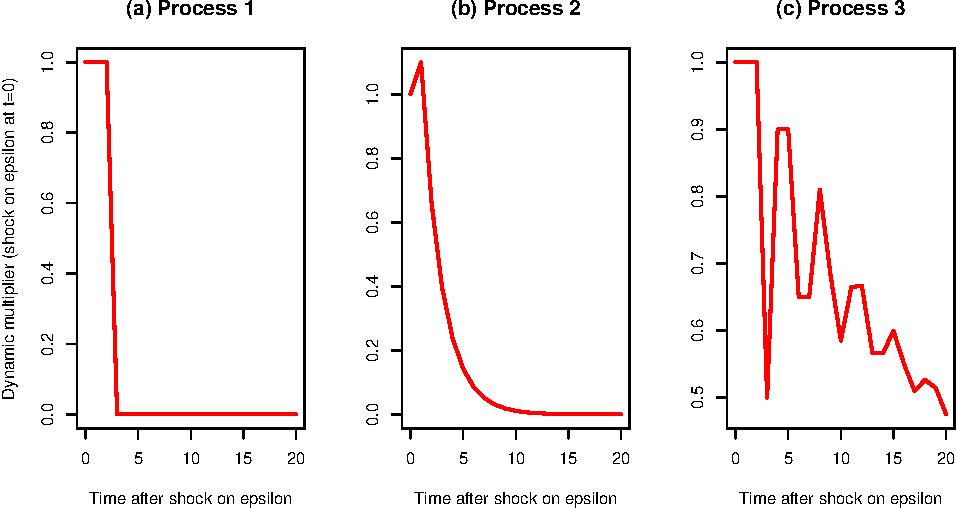
\includegraphics[width=1\linewidth]{TimeSeries_files/figure-latex/IRFarma-1} \caption{IRFs associated with the three processes. Process 1 (MA(2)): $y_t = \varepsilon_t + \varepsilon_{t-1} + \varepsilon_{t-2}$. Process 2 (ARMA(1,1)): $y_{t}=0.6y_{t-1} + \varepsilon_t + 0.5\varepsilon_{t-1}$. Process 3 (ARMA(4,2)): $y_{t}=0.5y_{t-3} + 0.4y_{t-4} + \varepsilon_t + \varepsilon_{t-1} + \varepsilon_{t-2}$.}\label{fig:IRFarma}
\end{figure}

Consider the annual Swiss GDP growth from the JST macro-history database. Let us first determine relevant orders for AR and MA processes using the (P)ACF approach.

\begin{Shaded}
\begin{Highlighting}[]
\FunctionTok{library}\NormalTok{(AEC)}
\FunctionTok{data}\NormalTok{(JST);data }\OtherTok{\textless{}{-}} \FunctionTok{subset}\NormalTok{(JST,iso}\SpecialCharTok{==}\StringTok{"CHE"}\NormalTok{)}
\FunctionTok{par}\NormalTok{(}\AttributeTok{plt=}\FunctionTok{c}\NormalTok{(.}\DecValTok{1}\NormalTok{,.}\DecValTok{95}\NormalTok{,.}\DecValTok{1}\NormalTok{,.}\DecValTok{95}\NormalTok{))}
\NormalTok{T }\OtherTok{\textless{}{-}} \FunctionTok{dim}\NormalTok{(data)[}\DecValTok{1}\NormalTok{]}
\NormalTok{growth }\OtherTok{\textless{}{-}} \FunctionTok{log}\NormalTok{(data}\SpecialCharTok{$}\NormalTok{gdp[}\DecValTok{2}\SpecialCharTok{:}\NormalTok{T]}\SpecialCharTok{/}\NormalTok{data}\SpecialCharTok{$}\NormalTok{gdp[}\DecValTok{1}\SpecialCharTok{:}\NormalTok{(T}\DecValTok{{-}1}\NormalTok{)])}
\FunctionTok{par}\NormalTok{(}\AttributeTok{mfrow=}\FunctionTok{c}\NormalTok{(}\DecValTok{3}\NormalTok{,}\DecValTok{1}\NormalTok{));}\FunctionTok{par}\NormalTok{(}\AttributeTok{plt=}\FunctionTok{c}\NormalTok{(.}\DecValTok{1}\NormalTok{,.}\DecValTok{95}\NormalTok{,.}\DecValTok{15}\NormalTok{,.}\DecValTok{95}\NormalTok{))}
\FunctionTok{plot}\NormalTok{(data}\SpecialCharTok{$}\NormalTok{year[}\DecValTok{2}\SpecialCharTok{:}\NormalTok{T],growth,}\AttributeTok{type=}\StringTok{"l"}\NormalTok{,}\AttributeTok{xlab=}\StringTok{""}\NormalTok{,}\AttributeTok{ylab=}\StringTok{""}\NormalTok{,}\AttributeTok{lwd=}\DecValTok{2}\NormalTok{)}
\FunctionTok{abline}\NormalTok{(}\AttributeTok{h=}\DecValTok{0}\NormalTok{,}\AttributeTok{lty=}\DecValTok{2}\NormalTok{)}
\FunctionTok{acf}\NormalTok{(growth);}\FunctionTok{pacf}\NormalTok{(growth)}
\end{Highlighting}
\end{Shaded}

\begin{figure}
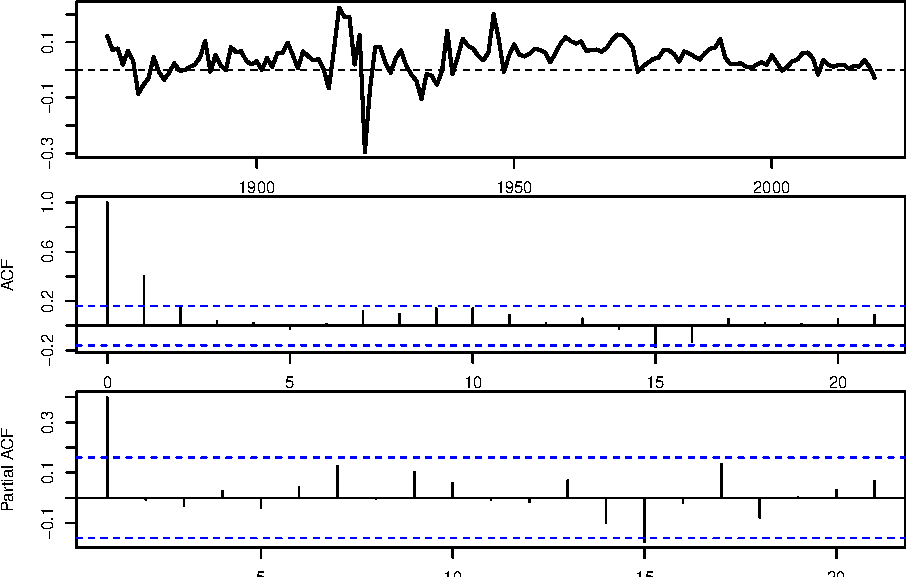
\includegraphics[width=1\linewidth]{TimeSeries_files/figure-latex/IRFgdp1-1} \caption{(P)ACF analysis of Swiss GDP growth.}\label{fig:IRFgdp1}
\end{figure}

The two bottom plots of Figure \ref{fig:IRFgdp1} suggest that either an MA(2) or an AR(1) could be used to model the GDP growth rate series. Figure \ref{fig:IRFgdp2} shows the IRFs based on these two respective specifications.

\begin{Shaded}
\begin{Highlighting}[]
\CommentTok{\# Fit an AR process:}
\NormalTok{res }\OtherTok{\textless{}{-}} \FunctionTok{arima}\NormalTok{(growth,}\AttributeTok{order=}\FunctionTok{c}\NormalTok{(}\DecValTok{1}\NormalTok{,}\DecValTok{0}\NormalTok{,}\DecValTok{0}\NormalTok{))}
\NormalTok{phi }\OtherTok{\textless{}{-}}\NormalTok{ res}\SpecialCharTok{$}\NormalTok{coef[}\DecValTok{1}\NormalTok{]}
\NormalTok{T }\OtherTok{\textless{}{-}} \DecValTok{11}
\NormalTok{y.sim }\OtherTok{\textless{}{-}} \FunctionTok{sim.arma}\NormalTok{(}\AttributeTok{c=}\DecValTok{0}\NormalTok{,phi,}\AttributeTok{theta=}\DecValTok{1}\NormalTok{,}\AttributeTok{sigma=}\DecValTok{1}\NormalTok{,T,}\AttributeTok{y.0=}\FunctionTok{rep}\NormalTok{(}\DecValTok{0}\NormalTok{,}\FunctionTok{length}\NormalTok{(phi)),}
                  \AttributeTok{nb.sim=}\DecValTok{1}\NormalTok{,}\AttributeTok{make.IRF =} \DecValTok{1}\NormalTok{)}
\FunctionTok{par}\NormalTok{(}\AttributeTok{plt=}\FunctionTok{c}\NormalTok{(.}\DecValTok{15}\NormalTok{,.}\DecValTok{95}\NormalTok{,.}\DecValTok{25}\NormalTok{,.}\DecValTok{95}\NormalTok{))}
\FunctionTok{plot}\NormalTok{(}\DecValTok{0}\SpecialCharTok{:}\NormalTok{(T}\DecValTok{{-}1}\NormalTok{),y.sim[,}\DecValTok{1}\NormalTok{],}\AttributeTok{type=}\StringTok{"l"}\NormalTok{,}\AttributeTok{lwd=}\DecValTok{3}\NormalTok{,}
     \AttributeTok{xlab=}\StringTok{"Time after shock on epsilon"}\NormalTok{,}
     \AttributeTok{ylab=}\StringTok{"Dynamic multiplier (shock on epsilon at t=0)"}\NormalTok{,}\AttributeTok{col=}\StringTok{"red"}\NormalTok{)}
\CommentTok{\# Fit a MA process:}
\NormalTok{res }\OtherTok{\textless{}{-}} \FunctionTok{arima}\NormalTok{(growth,}\AttributeTok{order=}\FunctionTok{c}\NormalTok{(}\DecValTok{0}\NormalTok{,}\DecValTok{0}\NormalTok{,}\DecValTok{2}\NormalTok{))}
\NormalTok{phi }\OtherTok{\textless{}{-}} \DecValTok{0}\NormalTok{;theta }\OtherTok{\textless{}{-}} \FunctionTok{c}\NormalTok{(}\DecValTok{1}\NormalTok{,res}\SpecialCharTok{$}\NormalTok{coef[}\DecValTok{1}\SpecialCharTok{:}\DecValTok{2}\NormalTok{])}
\NormalTok{y.sim }\OtherTok{\textless{}{-}} \FunctionTok{sim.arma}\NormalTok{(}\AttributeTok{c=}\DecValTok{0}\NormalTok{,phi,theta,}\AttributeTok{sigma=}\DecValTok{1}\NormalTok{,T,}\AttributeTok{y.0=}\FunctionTok{rep}\NormalTok{(}\DecValTok{0}\NormalTok{,}\FunctionTok{length}\NormalTok{(phi)),}
                  \AttributeTok{nb.sim=}\DecValTok{1}\NormalTok{,}\AttributeTok{make.IRF =} \DecValTok{1}\NormalTok{)}
\FunctionTok{lines}\NormalTok{(}\DecValTok{0}\SpecialCharTok{:}\NormalTok{(T}\DecValTok{{-}1}\NormalTok{),y.sim[,}\DecValTok{1}\NormalTok{],}\AttributeTok{lwd=}\DecValTok{3}\NormalTok{,}\AttributeTok{col=}\StringTok{"red"}\NormalTok{,}\AttributeTok{lty=}\DecValTok{2}\NormalTok{)}
\FunctionTok{abline}\NormalTok{(}\AttributeTok{h=}\DecValTok{0}\NormalTok{)}
\end{Highlighting}
\end{Shaded}

\begin{figure}
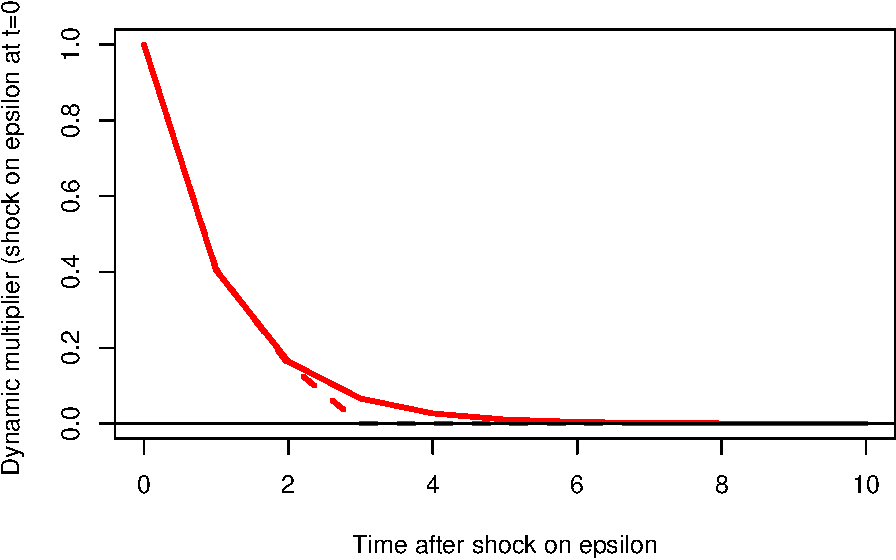
\includegraphics[width=1\linewidth]{TimeSeries_files/figure-latex/IRFgdp2-1} \caption{Dynamic response of Swiss annual growth to a shock on the innovation $\varepsilon_t$ at date $t=0$. The solid line corresponds to an AR(1) specification; the dashed line corresponds to a MA(2) specification.}\label{fig:IRFgdp2}
\end{figure}

The same kind of algorithm (as in Prop. \ref{prp:computPsi}) can be used to compute the impact of an increase in an exogenous variable \(x_t\) within an ARMAX(p,q,r) model (see next section).

\hypertarget{ARMAIRF}{%
\section{ARMA processes with exogenous variables (ARMA-X)}\label{ARMAIRF}}

ARMA processes do not allow to investigate the influence of an exogenous variable (say \(x_t\)) on the variable of interest (say \(y_t\)). When \(x_t\) and \(y_t\) have reciprocal influences, the Vector Autoregressive (VAR) model may be used (this tools will be studied later, in Section \ref{VAR}). However, when one suspects that \(x_t\) has an ``exogenous'' influence on \(y_t\), then a simple extension of the ARMA processes may be considered. Loosely speaking, \(x_t\) has an ``exogenous'' influence on \(y_t\) if \(y_t\) does not affect \(x_t\). This extension is referred to as ARMA-X.

To begin with, let us formalize this notion of exogeneity. Consider a white noise sequence \(\{\varepsilon_t\}\) (Def. \ref{def:whitenoise}). This white noise will enter the dynamics of \(y_t\), alongside with \(x_t\); but \(x_t\) will be exogenous to \(\varepsilon_t\). (We will also say that \(x_t\) is exogenous to \(y_t\).)

\begin{definition}[Exogeneity]
\protect\hypertarget{def:exogeneity}{}\label{def:exogeneity}We say that \(x_t\) is (strictly) exogenous to \(\{\varepsilon_t\}\) if
\[
\mathbb{E}(\varepsilon_t|\underbrace{\dots,x_{t+1}}_{\mbox{future}},\underbrace{x_t,x_{t-1},\dots}_{\mbox{present and past}}) = 0.
\]
\end{definition}

Hence, if \(\{x_t\}\) is strictly exogenous to \(\varepsilon_t\), then past, present and future values of \(x_t\) do not allow to predict the \(\varepsilon_t\)'s.

In the following, we assume that \(\{x_t\}\) is a covariance stationary process.

\begin{definition}[ARMAX(p,q,r) model]
\protect\hypertarget{def:ARMAX}{}\label{def:ARMAX}The process \(\{y_t\}\) is an ARMAX(p,q,r) if it follows a difference equation of the form:
\begin{eqnarray}
y_t &=& \underbrace{c + \phi_1 y_{t-1} + \dots + \phi_p y_{t-p}}_{\mbox{AR(p) part}} + \underbrace{\beta_0 x_t + \dots + \beta_{r} x_{t-r}}_{\mbox{X(r) part}} + \nonumber \\
&&\underbrace{\varepsilon_t + \theta_1\varepsilon_{t-1}+\dots +\theta_{q}\varepsilon_{t-q},}_{\mbox{MA(q) part}} \label{eq:DLM}
\end{eqnarray}
where \(\{\varepsilon_t\}\) is an i.i.d. white noise sequence and \(\{x_t\}\) is exogenous to \(y_t\).
\end{definition}

What is the effect of a one-unit increase in \(x_t\) on \(y_t\)? To address this question, this notion of ``effect'' has to be formalized. Let us introduce two related sequences of values for \(\{x\}\). Denote the first by \(\{a\}\) and the second by \(\{\tilde{a}^t\}\). Further, we posit \(a_s = \tilde{a}_s^t\) for all \(s \ne t\), and \(\tilde{a}_t^t = a_t+1\).

With these notations, we define \(\frac{\partial y_{t+h}}{\partial x_t}\) as follows:
\begin{equation}
\frac{\partial y_{t+h}}{\partial x_t} := \mathbb{E}_{t-1}(y_{t+h}|\{x\} = \{\tilde{a}^t\}) - \mathbb{E}_{t-1}(y_{t+h}|\{x\} = \{a\}).\label{eq:dynmultX}
\end{equation}
Under the exogeneity assumption, it is easily seen that

\[
\frac{\partial y_t}{\partial x_t} = \beta_0.
\]
Now, since
\begin{eqnarray*}
y_{t+1} &=& c + \phi_1 y_{t} + \dots + \phi_p y_{t+1-p} + \beta_0 x_{t+1} + \dots + \beta_{r} x_{t+1-r} +\\
&&\varepsilon_{t+1} + \theta_1\varepsilon_{t}+\dots +\theta_{q}\varepsilon_{t+1-q},
\end{eqnarray*}
and using the exogeneity assumption, we obtain:
\[
\frac{\partial y_{t+1}}{\partial x_t} := \phi_1 \frac{\partial y_{t}}{\partial x_t} + \beta_1 = \phi_1\beta_0 + \beta_1.
\]
This can be applied recursively to give \(\dfrac{\partial y_{t+h}}{\partial x_t}\) for any \(h \ge 0\):

\begin{proposition}[Dynamic multipliers in ARMAX models]
\protect\hypertarget{prp:computPsiARMAX}{}\label{prp:computPsiARMAX}

One can recursively compute the dynamic multipliers \(\frac{\partial y_{t+h}}{\partial x_t}\) as follows:

\begin{enumerate}
\def\labelenumi{\roman{enumi}.}
\tightlist
\item
  Initialization: \(\dfrac{\partial y_{t+h}}{\partial x_t}=0\) for \(h<0\).
\item
  For \(h \ge 0\) and assuming that the first \(h-1\) multipliers have been computed, we have:
  \begin{eqnarray}
  \dfrac{\partial y_{t+h}}{\partial x_t} &=& \phi_1 \dfrac{\partial y_{t+h-1}}{\partial x_t} + \dots + \phi_p \dfrac{\partial y_{t+h-p}}{\partial x_t} + \beta_h,\label{eq:dynmultX}
  \end{eqnarray}
  where we use the notation \(\beta_h=0\) if \(h>r\).
\end{enumerate}

\end{proposition}

Remark that the resulting dynamic multipliers are the same as those obtained for an ARMA(p,r) model where the \(\theta_i\)'s are replaced with \(\beta_i\)'s (see Proposition \ref{prp:computPsi} in Section \ref{ARMAIRF}).

It has to be stressed that the definition of the dynamic multipliers (Eq. \eqref{eq:dynmultX}) does not reflect a potential persistency of the shock occuring on date \(t\) in process \(\{x\}\) itself. Going in this direction would necessitate to model the joint dynamics of \(x_t\) (for instance using a VAR model, see Section \ref{VAR}).

\begin{example}[Influence of the number of freezing days on the price of orange juice]
\protect\hypertarget{exm:OrangeJuice}{}\label{exm:OrangeJuice}

This example is based on data used in \citet{Stock_Watson_2003} (Chapter 16). The objective is to study the influence of the number of freezing days on the price of orange juice. Let us first estimate a ARMAX(0,0,12) model:

\begin{Shaded}
\begin{Highlighting}[]
\FunctionTok{library}\NormalTok{(AEC);}\FunctionTok{library}\NormalTok{(AER)}
\FunctionTok{data}\NormalTok{(}\StringTok{"FrozenJuice"}\NormalTok{)}
\NormalTok{FJ }\OtherTok{\textless{}{-}} \FunctionTok{as.data.frame}\NormalTok{(FrozenJuice)}
\NormalTok{date }\OtherTok{\textless{}{-}} \FunctionTok{time}\NormalTok{(FrozenJuice)}
\NormalTok{price }\OtherTok{\textless{}{-}}\NormalTok{ FJ}\SpecialCharTok{$}\NormalTok{price}\SpecialCharTok{/}\NormalTok{FJ}\SpecialCharTok{$}\NormalTok{ppi}
\NormalTok{T }\OtherTok{\textless{}{-}} \FunctionTok{length}\NormalTok{(price)}
\NormalTok{k }\OtherTok{\textless{}{-}} \DecValTok{1}
\NormalTok{dprice }\OtherTok{\textless{}{-}} \DecValTok{100}\SpecialCharTok{*}\FunctionTok{log}\NormalTok{(price[(k}\SpecialCharTok{+}\DecValTok{1}\NormalTok{)}\SpecialCharTok{:}\NormalTok{T]}\SpecialCharTok{/}\NormalTok{price[}\DecValTok{1}\SpecialCharTok{:}\NormalTok{(T}\SpecialCharTok{{-}}\NormalTok{k)])}
\NormalTok{fdd }\OtherTok{\textless{}{-}}\NormalTok{ FJ}\SpecialCharTok{$}\NormalTok{fdd[(k}\SpecialCharTok{+}\DecValTok{1}\NormalTok{)}\SpecialCharTok{:}\NormalTok{T]}
\FunctionTok{par}\NormalTok{(}\AttributeTok{mfrow=}\FunctionTok{c}\NormalTok{(}\DecValTok{3}\NormalTok{,}\DecValTok{1}\NormalTok{))}
\FunctionTok{par}\NormalTok{(}\AttributeTok{plt=}\FunctionTok{c}\NormalTok{(.}\DecValTok{1}\NormalTok{,.}\DecValTok{95}\NormalTok{,.}\DecValTok{15}\NormalTok{,.}\DecValTok{75}\NormalTok{))}
\FunctionTok{plot}\NormalTok{(date,price,}\AttributeTok{type=}\StringTok{"l"}\NormalTok{,}\AttributeTok{xlab=}\StringTok{""}\NormalTok{,}\AttributeTok{ylab=}\StringTok{""}\NormalTok{,}
     \AttributeTok{main=}\StringTok{"(a) Price of orange Juice"}\NormalTok{)}
\FunctionTok{plot}\NormalTok{(date,}\FunctionTok{c}\NormalTok{(}\ConstantTok{NaN}\NormalTok{,dprice),}\AttributeTok{type=}\StringTok{"l"}\NormalTok{,}\AttributeTok{xlab=}\StringTok{""}\NormalTok{,}\AttributeTok{ylab=}\StringTok{""}\NormalTok{,}
     \AttributeTok{main=}\StringTok{"(b) Monthly pct Change (y)"}\NormalTok{)}
\FunctionTok{plot}\NormalTok{(date,FJ}\SpecialCharTok{$}\NormalTok{fdd,}\AttributeTok{type=}\StringTok{"l"}\NormalTok{,}\AttributeTok{xlab=}\StringTok{""}\NormalTok{,}\AttributeTok{ylab=}\StringTok{""}\NormalTok{,}
     \AttributeTok{main=}\StringTok{"(c) Number of freezing days (x)"}\NormalTok{)}
\end{Highlighting}
\end{Shaded}

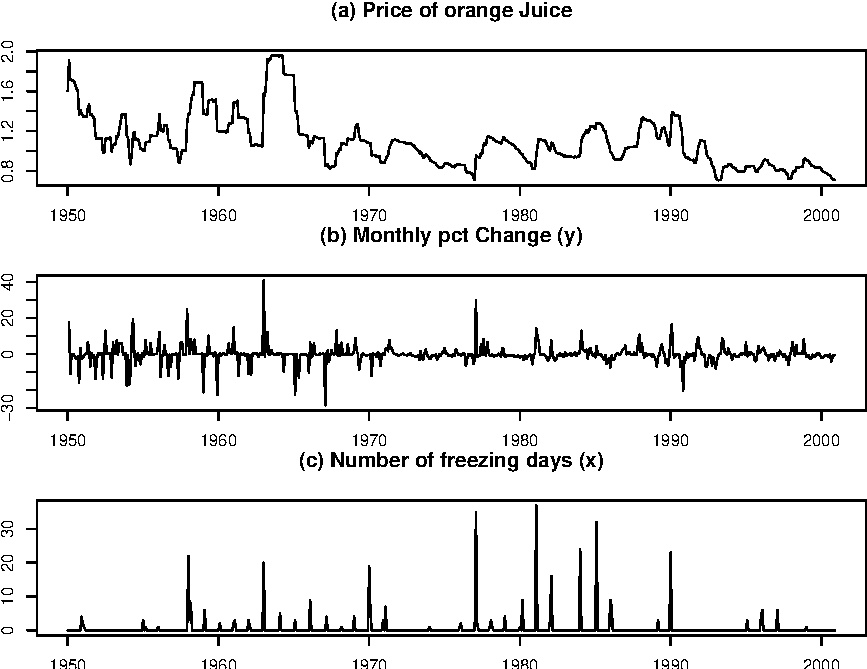
\includegraphics{TimeSeries_files/figure-latex/freez-1.pdf}

\begin{Shaded}
\begin{Highlighting}[]
\NormalTok{nb.lags }\OtherTok{\textless{}{-}} \DecValTok{3}
\NormalTok{FDD }\OtherTok{\textless{}{-}}\NormalTok{ FJ}\SpecialCharTok{$}\NormalTok{fdd[(nb.lags}\SpecialCharTok{+}\DecValTok{1}\NormalTok{)}\SpecialCharTok{:}\NormalTok{T]}
\NormalTok{names.FDD }\OtherTok{\textless{}{-}} \ConstantTok{NULL}
\ControlFlowTok{for}\NormalTok{(i }\ControlFlowTok{in} \DecValTok{1}\SpecialCharTok{:}\NormalTok{nb.lags)\{}
\NormalTok{  FDD }\OtherTok{\textless{}{-}} \FunctionTok{cbind}\NormalTok{(FDD,FJ}\SpecialCharTok{$}\NormalTok{fdd[(nb.lags}\SpecialCharTok{+}\DecValTok{1}\SpecialCharTok{{-}}\NormalTok{i)}\SpecialCharTok{:}\NormalTok{(T}\SpecialCharTok{{-}}\NormalTok{i)])}
\NormalTok{  names.FDD }\OtherTok{\textless{}{-}} \FunctionTok{c}\NormalTok{(names.FDD,}\FunctionTok{paste}\NormalTok{(}\StringTok{" Lag "}\NormalTok{,}\FunctionTok{toString}\NormalTok{(i),}\AttributeTok{sep=}\StringTok{""}\NormalTok{))\}}
\FunctionTok{colnames}\NormalTok{(FDD) }\OtherTok{\textless{}{-}} \FunctionTok{c}\NormalTok{(}\StringTok{" Lag 0"}\NormalTok{,names.FDD)}
\NormalTok{dprice }\OtherTok{\textless{}{-}}\NormalTok{ dprice[(}\FunctionTok{length}\NormalTok{(dprice)}\SpecialCharTok{{-}}\FunctionTok{dim}\NormalTok{(FDD)[}\DecValTok{1}\NormalTok{]}\SpecialCharTok{+}\DecValTok{1}\NormalTok{)}\SpecialCharTok{:}\FunctionTok{length}\NormalTok{(dprice)]}
\NormalTok{eq }\OtherTok{\textless{}{-}} \FunctionTok{lm}\NormalTok{(dprice}\SpecialCharTok{\textasciitilde{}}\NormalTok{FDD)}
\CommentTok{\# Compute the Newey{-}West std errors:}
\NormalTok{var.cov.mat }\OtherTok{\textless{}{-}} \FunctionTok{NeweyWest}\NormalTok{(eq,}\AttributeTok{lag =} \DecValTok{7}\NormalTok{, }\AttributeTok{prewhite =} \ConstantTok{FALSE}\NormalTok{)}
\NormalTok{robust\_se }\OtherTok{\textless{}{-}} \FunctionTok{sqrt}\NormalTok{(}\FunctionTok{diag}\NormalTok{(var.cov.mat))}
\CommentTok{\# Stargazer output (with and without Robust SE)}
\NormalTok{stargazer}\SpecialCharTok{::}\FunctionTok{stargazer}\NormalTok{(eq, eq, }\AttributeTok{type =} \StringTok{"text"}\NormalTok{,}
                     \AttributeTok{column.labels=}\FunctionTok{c}\NormalTok{(}\StringTok{"(no HAC)"}\NormalTok{,}\StringTok{"(HAC)"}\NormalTok{),}\AttributeTok{keep.stat=}\StringTok{"n"}\NormalTok{,}
                     \AttributeTok{se =} \FunctionTok{list}\NormalTok{(}\ConstantTok{NULL}\NormalTok{,robust\_se),}\AttributeTok{no.space =} \ConstantTok{TRUE}\NormalTok{)}
\end{Highlighting}
\end{Shaded}

\begin{verbatim}
## 
## =========================================
##                  Dependent variable:     
##              ----------------------------
##                         dprice           
##                 (no HAC)        (HAC)    
##                   (1)            (2)     
## -----------------------------------------
## FDD Lag 0       0.467***      0.467***   
##                 (0.057)        (0.135)   
## FDD Lag 1       0.140**        0.140*    
##                 (0.057)        (0.083)   
## FDD Lag 2        0.055          0.055    
##                 (0.057)        (0.056)   
## FDD Lag 3        0.073          0.073    
##                 (0.057)        (0.047)   
## Constant       -0.599***      -0.599***  
##                 (0.204)        (0.213)   
## -----------------------------------------
## Observations      609            609     
## =========================================
## Note:         *p<0.1; **p<0.05; ***p<0.01
\end{verbatim}

Let us now use function \texttt{estim.armax}, from package \texttt{AEC}to fit an ARMA-X(2,0,1) model:

\begin{Shaded}
\begin{Highlighting}[]
\NormalTok{nb.lags.exog }\OtherTok{\textless{}{-}} \DecValTok{1} \CommentTok{\# number of lags of exog. variable}
\NormalTok{FDD }\OtherTok{\textless{}{-}}\NormalTok{ FJ}\SpecialCharTok{$}\NormalTok{fdd[(nb.lags.exog}\SpecialCharTok{+}\DecValTok{1}\NormalTok{)}\SpecialCharTok{:}\NormalTok{T]}
\ControlFlowTok{for}\NormalTok{(i }\ControlFlowTok{in} \DecValTok{1}\SpecialCharTok{:}\NormalTok{nb.lags.exog)\{}
\NormalTok{  FDD }\OtherTok{\textless{}{-}} \FunctionTok{cbind}\NormalTok{(FDD,FJ}\SpecialCharTok{$}\NormalTok{fdd[(nb.lags.exog}\SpecialCharTok{+}\DecValTok{1}\SpecialCharTok{{-}}\NormalTok{i)}\SpecialCharTok{:}\NormalTok{(T}\SpecialCharTok{{-}}\NormalTok{i)])\}}
\NormalTok{dprice }\OtherTok{\textless{}{-}} \DecValTok{100}\SpecialCharTok{*}\FunctionTok{log}\NormalTok{(price[(k}\SpecialCharTok{+}\DecValTok{1}\NormalTok{)}\SpecialCharTok{:}\NormalTok{T]}\SpecialCharTok{/}\NormalTok{price[}\DecValTok{1}\SpecialCharTok{:}\NormalTok{(T}\SpecialCharTok{{-}}\NormalTok{k)])}
\NormalTok{dprice }\OtherTok{\textless{}{-}}\NormalTok{ dprice[(}\FunctionTok{length}\NormalTok{(dprice)}\SpecialCharTok{{-}}\FunctionTok{dim}\NormalTok{(FDD)[}\DecValTok{1}\NormalTok{]}\SpecialCharTok{+}\DecValTok{1}\NormalTok{)}\SpecialCharTok{:}\FunctionTok{length}\NormalTok{(dprice)]}
\NormalTok{res.armax }\OtherTok{\textless{}{-}} \FunctionTok{estim.armax}\NormalTok{(}\AttributeTok{Y =}\NormalTok{ dprice,}\AttributeTok{p=}\DecValTok{3}\NormalTok{,}\AttributeTok{q=}\DecValTok{0}\NormalTok{,}\AttributeTok{X=}\NormalTok{FDD)}
\end{Highlighting}
\end{Shaded}

\begin{verbatim}
## [1] "=================================================="
## [1] "  ESTIMATING"
## [1] "=================================================="
## [1] "  END OF ESTIMATION"
## [1] "=================================================="
## [1] ""
## [1] "  RESULTS:"
## [1] "  -----------------------"
##                 THETA     st.dev   t.ratio
## c         -0.46556249 0.19554352 -2.380864
## phi   t-1  0.09788977 0.04025907  2.431496
## phi   t-2  0.05049849 0.03827488  1.319364
## phi   t-3  0.07155170 0.03764750  1.900570
## sigma      4.64917949 0.13300769 34.954215
## beta  t-0  0.47015552 0.05665344  8.298800
## beta  t-1  0.10015862 0.05972526  1.676989
## [1] "=================================================="
\end{verbatim}

Figure \ref{fig:freez4} shows the IRF associated with each of the two models.

\begin{Shaded}
\begin{Highlighting}[]
\NormalTok{nb.periods }\OtherTok{\textless{}{-}} \DecValTok{20}
\NormalTok{IRF1 }\OtherTok{\textless{}{-}} \FunctionTok{sim.arma}\NormalTok{(}\AttributeTok{c=}\DecValTok{0}\NormalTok{,}\AttributeTok{phi=}\FunctionTok{c}\NormalTok{(}\DecValTok{0}\NormalTok{),}\AttributeTok{theta=}\NormalTok{eq}\SpecialCharTok{$}\NormalTok{coefficients[}\DecValTok{2}\SpecialCharTok{:}\NormalTok{(nb.lags}\SpecialCharTok{+}\DecValTok{1}\NormalTok{)],}\AttributeTok{sigma=}\DecValTok{1}\NormalTok{,}
                 \AttributeTok{T=}\NormalTok{nb.periods,}\AttributeTok{y.0=}\FunctionTok{c}\NormalTok{(}\DecValTok{0}\NormalTok{),}\AttributeTok{nb.sim=}\DecValTok{1}\NormalTok{,}\AttributeTok{make.IRF=}\DecValTok{1}\NormalTok{)}
\NormalTok{IRF2 }\OtherTok{\textless{}{-}} \FunctionTok{sim.arma}\NormalTok{(}\AttributeTok{c=}\DecValTok{0}\NormalTok{,}\AttributeTok{phi=}\NormalTok{res.armax}\SpecialCharTok{$}\NormalTok{phi,}\AttributeTok{theta=}\NormalTok{res.armax}\SpecialCharTok{$}\NormalTok{beta,}\AttributeTok{sigma=}\DecValTok{1}\NormalTok{,}
                 \AttributeTok{T=}\NormalTok{nb.periods,}\AttributeTok{y.0=}\FunctionTok{rep}\NormalTok{(}\DecValTok{0}\NormalTok{,}\FunctionTok{length}\NormalTok{(res.armax}\SpecialCharTok{$}\NormalTok{phi)),}
                 \AttributeTok{nb.sim=}\DecValTok{1}\NormalTok{,}\AttributeTok{make.IRF=}\DecValTok{1}\NormalTok{)}
\FunctionTok{par}\NormalTok{(}\AttributeTok{plt=}\FunctionTok{c}\NormalTok{(.}\DecValTok{15}\NormalTok{,.}\DecValTok{95}\NormalTok{,.}\DecValTok{2}\NormalTok{,.}\DecValTok{95}\NormalTok{))}
\FunctionTok{plot}\NormalTok{(IRF1,}\AttributeTok{type=}\StringTok{"l"}\NormalTok{,}\AttributeTok{lwd=}\DecValTok{2}\NormalTok{,}\AttributeTok{col=}\StringTok{"red"}\NormalTok{,}\AttributeTok{xlab=}\StringTok{"months after shock"}\NormalTok{,}
     \AttributeTok{ylab=}\StringTok{"Chge in price (percent)"}\NormalTok{)}
\FunctionTok{lines}\NormalTok{(IRF2,}\AttributeTok{lwd=}\DecValTok{2}\NormalTok{,}\AttributeTok{col=}\StringTok{"red"}\NormalTok{,}\AttributeTok{lty=}\DecValTok{2}\NormalTok{)}
\FunctionTok{abline}\NormalTok{(}\AttributeTok{h=}\DecValTok{0}\NormalTok{,}\AttributeTok{col=}\StringTok{"grey"}\NormalTok{)}
\end{Highlighting}
\end{Shaded}

\begin{figure}
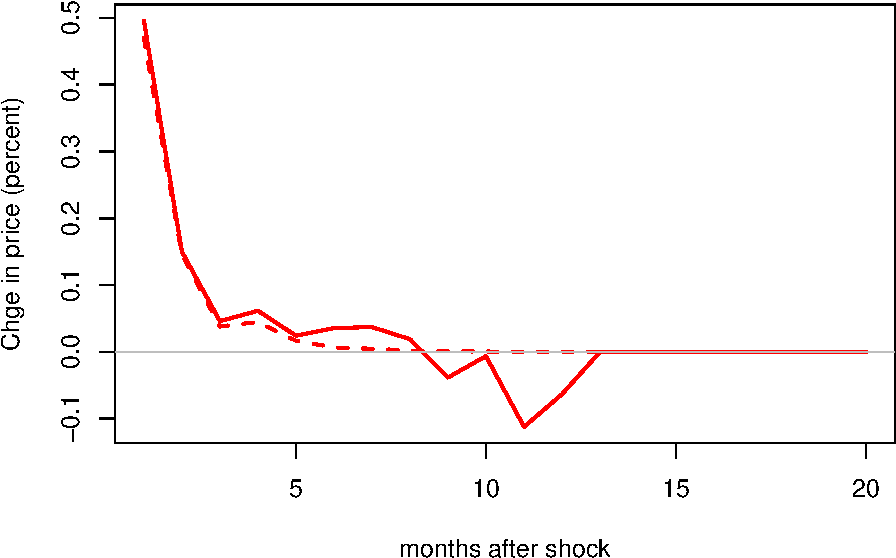
\includegraphics[width=0.95\linewidth]{TimeSeries_files/figure-latex/freez4-1} \caption{Response of changes in orange juice price (in percent) to the number of freezing days. The solid (respectively dashed) line corresponds to the ARMAX(0,0,3) (resp. ARMAX(3,0,1)) model. The first model is estimated by OLS (see above), the second by MLE.}\label{fig:freez4}
\end{figure}

\end{example}

\begin{example}[Real effect of a monetary policy shock]
\protect\hypertarget{exm:Ramey1}{}\label{exm:Ramey1}

In this example, we make use of monetary shocks identified through high-frequency data (see \citet{Gertler_Karadi_2015}). This dataset comes from \href{https://econweb.ucsd.edu/~vramey/research.html}{Valerie Ramey's website} (see \citet{Ramey_2016_NBER}).

\begin{Shaded}
\begin{Highlighting}[]
\FunctionTok{library}\NormalTok{(AEC)}
\NormalTok{T }\OtherTok{\textless{}{-}} \FunctionTok{dim}\NormalTok{(Ramey)[}\DecValTok{1}\NormalTok{]}
\CommentTok{\# Construct growth series:}
\NormalTok{Ramey}\SpecialCharTok{$}\NormalTok{growth }\OtherTok{\textless{}{-}}\NormalTok{ Ramey}\SpecialCharTok{$}\NormalTok{LIP }\SpecialCharTok{{-}} \FunctionTok{c}\NormalTok{(}\FunctionTok{rep}\NormalTok{(}\ConstantTok{NaN}\NormalTok{,}\DecValTok{12}\NormalTok{),Ramey}\SpecialCharTok{$}\NormalTok{LIP[}\DecValTok{1}\SpecialCharTok{:}\NormalTok{(}\FunctionTok{length}\NormalTok{(Ramey}\SpecialCharTok{$}\NormalTok{LIP)}\SpecialCharTok{{-}}\DecValTok{12}\NormalTok{)])}
\CommentTok{\# Prepare matrix of exogenous variables:}
\NormalTok{vec.lags }\OtherTok{\textless{}{-}} \FunctionTok{c}\NormalTok{(}\DecValTok{9}\NormalTok{,}\DecValTok{12}\NormalTok{,}\DecValTok{18}\NormalTok{)}
\NormalTok{Matrix.of.Exog }\OtherTok{\textless{}{-}} \ConstantTok{NULL}
\NormalTok{shocks }\OtherTok{\textless{}{-}}\NormalTok{ Ramey}\SpecialCharTok{$}\NormalTok{ED2\_TC}
\ControlFlowTok{for}\NormalTok{(i }\ControlFlowTok{in} \DecValTok{1}\SpecialCharTok{:}\FunctionTok{length}\NormalTok{(vec.lags))\{Matrix.of.Exog }\OtherTok{\textless{}{-}}
  \FunctionTok{cbind}\NormalTok{(Matrix.of.Exog,}\FunctionTok{c}\NormalTok{(}\FunctionTok{rep}\NormalTok{(}\ConstantTok{NaN}\NormalTok{,vec.lags[i]),shocks[}\DecValTok{1}\SpecialCharTok{:}\NormalTok{(T}\SpecialCharTok{{-}}\NormalTok{vec.lags[i])]))\}}
\CommentTok{\# Look for dates where data are available:}
\NormalTok{indic.good.dates }\OtherTok{\textless{}{-}} \FunctionTok{complete.cases}\NormalTok{(Matrix.of.Exog)}
\end{Highlighting}
\end{Shaded}

\begin{figure}
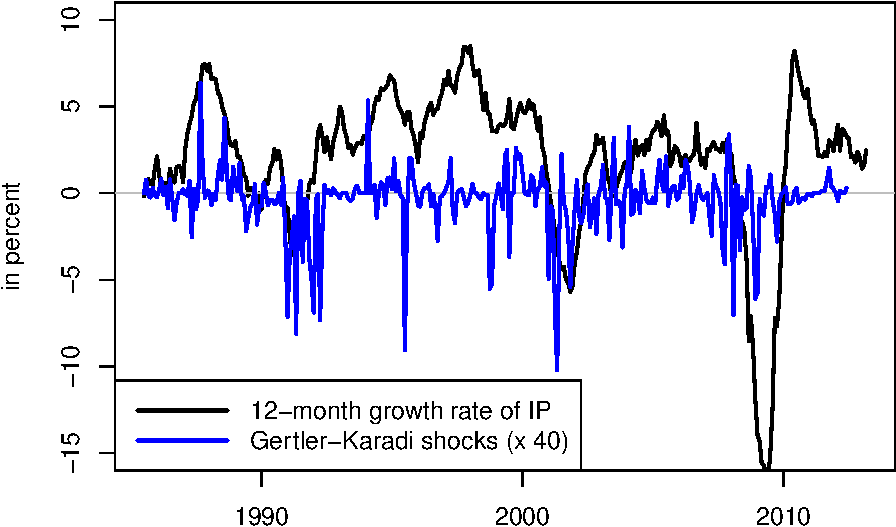
\includegraphics[width=0.95\linewidth]{TimeSeries_files/figure-latex/Ramey1fig-1} \caption{The blue line corresponds to monetary-policy shocks identified by means of the Gertler and Karadi (2015)'s approach (high-frequency change in Euro-dollar futures). The black slid line is the year-on-year growth rate of industrial production.}\label{fig:Ramey1fig}
\end{figure}

\begin{Shaded}
\begin{Highlighting}[]
\CommentTok{\# Estimate ARMAX:}
\NormalTok{p }\OtherTok{\textless{}{-}} \DecValTok{1}\NormalTok{; q }\OtherTok{\textless{}{-}} \DecValTok{0}
\NormalTok{x }\OtherTok{\textless{}{-}} \FunctionTok{estim.armax}\NormalTok{(Ramey}\SpecialCharTok{$}\NormalTok{growth[indic.good.dates],p,q,}
                 \AttributeTok{X=}\NormalTok{Matrix.of.Exog[indic.good.dates,])}
\end{Highlighting}
\end{Shaded}

\begin{verbatim}
## [1] "=================================================="
## [1] "  ESTIMATING"
## [1] "=================================================="
## [1] "  END OF ESTIMATION"
## [1] "=================================================="
## [1] ""
## [1] "  RESULTS:"
## [1] "  -----------------------"
##                   THETA       st.dev    t.ratio
## c         -0.0001716198 0.0005845907 -0.2935726
## phi   t-1  0.9825608412 0.0120458531 81.5683897
## sigma      0.0087948724 0.0003211748 27.3834438
## beta  t-0 -0.0193570616 0.0087331529 -2.2165032
## beta  t-1 -0.0225707935 0.0086750938 -2.6017925
## beta  t-2 -0.0070131593 0.0086387440 -0.8118263
## [1] "=================================================="
\end{verbatim}

\begin{Shaded}
\begin{Highlighting}[]
\CommentTok{\# Compute IRF:}
\NormalTok{irf }\OtherTok{\textless{}{-}} \FunctionTok{sim.arma}\NormalTok{(}\DecValTok{0}\NormalTok{,x}\SpecialCharTok{$}\NormalTok{phi,x}\SpecialCharTok{$}\NormalTok{beta,x}\SpecialCharTok{$}\NormalTok{sigma,}\AttributeTok{T=}\DecValTok{60}\NormalTok{,}\AttributeTok{y.0=}\FunctionTok{rep}\NormalTok{(}\DecValTok{0}\NormalTok{,}\FunctionTok{length}\NormalTok{(x}\SpecialCharTok{$}\NormalTok{phi)),}
                \AttributeTok{nb.sim=}\DecValTok{1}\NormalTok{,}\AttributeTok{make.IRF=}\DecValTok{1}\NormalTok{,}\AttributeTok{X=}\ConstantTok{NaN}\NormalTok{,}\AttributeTok{beta=}\ConstantTok{NaN}\NormalTok{)}
\end{Highlighting}
\end{Shaded}

Figure \ref{fig:Ramey3} displays the resulting IRF, with a 95\% confidence band. The code used to produce the confidence bands (i.e., to compute the standard deviation of the dynamic multipliers for the different horizons) is based on the Delta method (see Appendix \ref{Delta}).\footnote{This method consists in approximating \(\mathbb{V}(ar)(f(\theta))\) with \(\frac{\partial f(\theta)}{\partial \theta}' \mathbb{V}ar(\theta)\frac{\partial f(\theta)}{\partial \theta}\).}

\begin{figure}
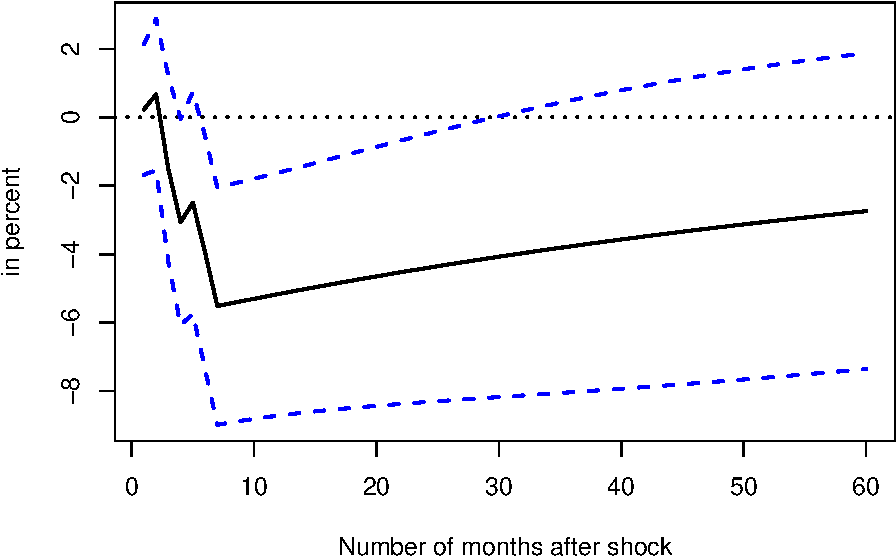
\includegraphics[width=0.95\linewidth]{TimeSeries_files/figure-latex/Ramey3-1} \caption{Response of industrial-production growth to monetary-policy shocks. Dashed lines correpsond to the $\pm$  2-standard-deviation bands.}\label{fig:Ramey3}
\end{figure}

\end{example}

\hypertarget{estimARMA}{%
\section{Maximum Likelihood Estimation (MLE) of ARMA processes}\label{estimARMA}}

Consider the general case (of any time series); assume we observe a sample \(\mathbf{y}=[y_1,\dots,y_T]'\). In order to implement ML techniques, we need to evaluate the joint p.d.f. (or ``likelihood'') of \(\mathbf{y}\), i.e., \(\mathcal{L}(\boldsymbol\theta;\mathbf{y})\), where \(\boldsymbol\theta\) is a vector of parameters that characterizes the dynamics of \(y_t\). The Maximum Likelihood (ML) estimate of \(\boldsymbol\theta\) is then given by:
\[
\boxed{\boldsymbol\theta_{MLE} = \arg \max_{\boldsymbol\theta} \mathcal{L}(\boldsymbol\theta;\mathbf{y})  = \arg \max_{\boldsymbol\theta} \log \mathcal{L}(\boldsymbol\theta;\mathbf{y}).}
\]

In the time series context, if process \(y_t\) is Markovian, then there exists a useful way to rewrite the likelihood \(\mathcal{L}(\boldsymbol\theta;\mathbf{y})\). Let us first recall the definition of a Markovian process:

\begin{definition}[Markovian process]
\protect\hypertarget{def:Markov}{}\label{def:Markov}Process \(y_t\) is Markovian of order one if \(f_{Y_t|Y_{t-1},Y_{t-2},\dots} = f_{Y_t|Y_{t-1}}\). More generally, it is Markovian of order \(k\) if \(f_{Y_t|Y_{t-1},Y_{t-2},\dots} = f_{Y_t|Y_{t-1},\dots,Y_{t-k}}\).
\end{definition}

Now, remember Bayes' formula:
\[
\mathbb{P}(X_2=x,X_1=y) = \mathbb{P}(X_2=x|X_1=y)\mathbb{P}(X_1=y).
\]
Using it leads to the following decomposition of our likelihood function:
\begin{eqnarray*}
f_{Y_T,\dots,Y_1}(y_T,\dots,y_1;\boldsymbol\theta) &=&f_{Y_T|Y_{T-1},\dots,Y_1}(y_T,\dots,y_1;\boldsymbol\theta) \times \\
&& f_{Y_{T-1},\dots,Y_1}(y_{T-1},\dots,y_1;\boldsymbol\theta).
\end{eqnarray*}
Using the previous expression recursively, one obtains:
\begin{equation}
f_{Y_T,\dots,Y_1}(y_T,\dots,y_1;\boldsymbol\theta) = f_{Y_1}(y_1;\boldsymbol\theta) \prod_{t=2}^{T} f_{Y_t|Y_{t-1},\dots,Y_1}(y_t,\dots,y_1;\boldsymbol\theta).\label{eq:recursMLE}
\end{equation}

Let us start with the Gaussian AR(1) process (which is Markovian of order one):
\[
y_t = c + \phi_1 y_{t-1} + \varepsilon_t, \quad \varepsilon_t \sim\,i.i.d.\, \mathcal{N}(0,\sigma^2).
\]
For \(t>1\):
\[
f_{Y_t|Y_{t-1},\dots,Y_1}(y_t,\dots,y_1;\boldsymbol\theta) = f_{Y_t|Y_{t-1}}(y_t,y_{t-1};\boldsymbol\theta)
\]
and
\[
f_{Y_t|Y_{t-1}}(y_t,y_{t-1};\boldsymbol\theta) = \frac{1}{\sqrt{2\pi}\sigma}\exp\left(-\frac{(y_t - c - \phi_1 y_{t-1})^2}{2\sigma^2}\right).
\]

These expressions can be plugged into Eq. \eqref{eq:recursMLE}. But what about \(f_{Y_1}(y_1;\boldsymbol\theta)\)? There exist two possibilities:

\begin{enumerate}
\def\labelenumi{\arabic{enumi}.}
\tightlist
\item
  \textbf{Case 1}: We use the marginal distribution: \(y_1 \sim \mathcal{N}\left(\dfrac{c}{1-\phi_1},\dfrac{\sigma^2}{1-\phi_1^2}\right)\).
\item
  \textbf{Case 2}: \(y_1\) is considered to be deterministic. In a way, that means that the first observation is ``sacrificed''.
\end{enumerate}

For a Gaussian AR(1) process, we have:

\begin{enumerate}
\def\labelenumi{\arabic{enumi}.}
\item
  \textbf{Case 1}: The (exact) log-likelihood is:
  \begin{eqnarray}
  \log \mathcal{L}(\boldsymbol\theta;\mathbf{y})  &=& - \frac{T}{2} \log(2\pi) - T\log(\sigma) + \frac{1}{2}\log(1-\phi_1^2)\nonumber \\
  && - \frac{(y_1 - c/(1-\phi_1))^2}{2\sigma^2/(1-\phi_1^2)} - \sum_{t=2}^T \left[\frac{(y_t - c - \phi_1 y_{t-1})^2}{2\sigma^2} \right].
  \end{eqnarray}
  The Maximum Likelihood Estimator of \(\boldsymbol\theta= [c,\phi_1,\sigma^2]\) is obtained by numerical optimization.
\item
  \textbf{Case 2}: The (conditional) log-likelihood is:
  \begin{eqnarray}
  \log \mathcal{L}^*(\boldsymbol\theta;\mathbf{y})  &=& - \frac{T-1}{2} \log(2\pi) - (T-1)\log(\sigma)\nonumber\\
  && - \sum_{t=2}^T \left[\frac{(y_t - c - \phi_1 y_{t-1})^2}{2\sigma^2} \right].\label{eq:Lstar}
  \end{eqnarray}
\end{enumerate}

Exact MLE and conditional MLE have the same asymptotic (i.e.~large-sample) distribution. Indeed, when the process is stationary, \(f_{Y_1}(y_1;\boldsymbol\theta)\) makes a relatively negligible contribution to \(\log \mathcal{L}(\boldsymbol\theta;\mathbf{y})\).

The conditional MLE has a substantial advantage: in the Gaussian case, the conditional MLE is simply obtained by OLS. Indeed, let us introduce the notations:
\[
Y = \left[\begin{array}{c}
y_2\\
\vdots\\
y_T
\end{array}\right] \quad and \quad
X = \left[\begin{array}{cc}
1 &y_1\\
\vdots&\vdots\\
1&y_{T-1}
\end{array}\right].
\]
Eq. \eqref{eq:Lstar} then rewrites:
\begin{eqnarray}
\log \mathcal{L}^*(\boldsymbol\theta;\mathbf{y})  &=& - \frac{T-1}{2} \log(2\pi) - (T-1)\log(\sigma) \nonumber \\
&& - \frac{1}{2\sigma^2} (Y-X[c,\phi_1]')'(Y-X[c,\phi_1]'),
\end{eqnarray}
which is maximised for:
\begin{eqnarray}
[\hat{c},\hat\phi_1]' &=& (X'X)^{-1}X'Y \label{eq:AROLSmean} \\
\hat{\sigma^2} &=& \frac{1}{T-1} \sum_{t=2}^T (y_t - \hat{c} - \hat{\phi_1}y_{t-1})^2 \nonumber \\
&=& \frac{1}{T-1} Y'(I - X(X'X)^{-1}X')Y. \label{eq:AROLSsigma}
\end{eqnarray}

Let us turn to the case of an AR(p) process. We have:
\begin{eqnarray*}
\log \mathcal{L}(\boldsymbol\theta;\mathbf{y}) &=& \log f_{Y_p,\dots,Y_1}(y_p,\dots,y_1;\boldsymbol\theta) +\\
&& \underbrace{\sum_{t=p+1}^{T} \log f_{Y_t|Y_{t-1},\dots,Y_{t-p}}(y_t,\dots,y_{t-p};\boldsymbol\theta)}_{\log \mathcal{L}^*(\boldsymbol\theta;\mathbf{y})}.
\end{eqnarray*}
where \(f_{Y_p,\dots,Y_{1}}(y_p,\dots,y_{1};\boldsymbol\theta)\) is the marginal distribution of \(\mathbf{y}_{1:p} := [y_p,\dots,y_1]'\). The marginal distribution of \(\mathbf{y}_{1:p}\) is Gaussian; it is therefore fully characterised by its mean and covariance matrix:
\begin{eqnarray*}
\mathbb{E}(\mathbf{y}_{1:p})&=&\frac{c}{1-\phi_1-\dots-\phi_p} \mathbf{1}_{p\times 1} \\
\mathbb{V}ar(\mathbf{y}_{1:p}) &=& \left[\begin{array}{cccc}
\gamma_0 & \gamma_1 & \dots & \gamma_{p-1} \\
\gamma_1 & \gamma_0 & \dots & \gamma_{p-2} \\
\vdots &  & \ddots & \vdots \\
\gamma_{p-1} & \gamma_{p-2} & \dots & \gamma_{0} \\
\end{array}\right],
\end{eqnarray*}
where the \(\gamma_i\)'s are computed using the Yule-Walker equations (Eq. \eqref{eq:gammas}). Note that they depend, in a non-linear way, on the model parameters. Hence, the maximization of the exact log-likelihood necessitates numerical oprimization procedures. By contrast, the maximization of the conditional log-likelihood \(\log \mathcal{L}^*(\boldsymbol\theta;\mathbf{y})\) only requires OLS, using Eqs. \eqref{eq:AROLSmean} and \eqref{eq:AROLSsigma}, with:
\[
Y = \left[\begin{array}{c}
y_{p+1}\\
\vdots\\
y_T
\end{array}\right] \quad and \quad
X = \left[\begin{array}{cccc}
1 & y_p & \dots & y_1\\
\vdots&\vdots&&\vdots\\
1&y_{T-1}&\dots&y_{T-p}
\end{array}\right].
\]

Again, for stationary processes, conditional and exact MLE have the same asymptotic (large-sample) distribution. In small samples, the OLS formula is however biased. Indeed, consider the regression (where \(y_t\) follows an AR(p) process):
\begin{equation}
y_t = \boldsymbol\beta'\mathbf{x}_t + \varepsilon_t,\label{eq:OLSregARp}
\end{equation}
with \(\mathbf{x}_t = [1,y_{t-1},\dots,y_{t-p}]'\) and \(\boldsymbol\beta = [c,\phi_1,\dots,\phi_p]'\).

The bias results from the fact that \(\mathbf{x}_t\) correlates to the \(\varepsilon_s\)'s for \(s<t\). To be sure:
\begin{equation}
\mathbf{b} = \boldsymbol{\beta} + (X'X)^{-1}X'\boldsymbol\varepsilon,\label{eq:olsar1}
\end{equation}
and because of the specific form of \(X\), we have non-zero correlation between \(\mathbf{x}_t\) and \(\varepsilon_s\) for \(s<t\), therefore \(\mathbb{E}[(X'X)^{-1}X'\boldsymbol\varepsilon] \ne 0\). Again, asymptotically, the previous expectation goes to zero, and we have:

\begin{proposition}[Large-sample porperties of the OLS estimator of AR(p) models]
\protect\hypertarget{prp:cgceOLSARp}{}\label{prp:cgceOLSARp}Assume \(\{y_t\}\) follows the AR(p) process:
\[
y_t = c + \phi_1 y_{t-1} + \dots + \phi_p y_{t-p} + \varepsilon_t
\]
where \(\{\varepsilon_{t}\}\) is an i.i.d. white noise process. If \(\mathbf{b}\) is the OLS estimator of \(\boldsymbol\beta\) (Eq. \eqref{eq:OLSregARp}), we have:
\[
\sqrt{T}(\mathbf{b}-\boldsymbol{\beta}) =  \underbrace{\left[\frac{1}{T}\sum_{t=p}^T \mathbf{x}_t\mathbf{x}_t' \right]^{-1}}_{\overset{p}{\rightarrow} \mathbf{Q}^{-1}}
\underbrace{\sqrt{T} \left[\frac{1}{T}\sum_{t=1}^T \mathbf{x}_t\varepsilon_t \right]}_{\overset{d}{\rightarrow} \mathcal{N}(0,\sigma^2\mathbf{Q})},
\]
where \(\mathbf{Q} = \mbox{plim }\frac{1}{T}\sum_{t=p}^T \mathbf{x}_t\mathbf{x}_t'= \mbox{plim }\frac{1}{T}\sum_{t=1}^T \mathbf{x}_t\mathbf{x}_t'\) is given by:
\begin{equation}
\mathbf{Q} = \left[
\begin{array}{ccccc}
1 & \mu &\mu & \dots & \mu \\
\mu & \gamma_0 + \mu^2 & \gamma_1 + \mu^2 & \dots & \gamma_{p-1} + \mu^2\\
\mu & \gamma_1 + \mu^2 & \gamma_0 + \mu^2 & \dots & \gamma_{p-2} + \mu^2\\
\vdots &\vdots &\vdots &\dots &\vdots \\
\mu & \gamma_{p-1} + \mu^2 & \gamma_{p-2} + \mu^2 & \dots & \gamma_{0} + \mu^2
\end{array}
\right].\label{eq:Qols}
\end{equation}
\end{proposition}

\begin{proof}
Rearranging Eq. \eqref{eq:olsar1}, we have:
\[
\sqrt{T}(\mathbf{b}-\boldsymbol{\beta}) =  (X'X/T)^{-1}\sqrt{T}(X'\boldsymbol\varepsilon/T).
\]
Let us consider the autocovariances of \(\mathbf{v}_t = \mathbf{x}_t \varepsilon_t\), denoted by \(\gamma^v_j\). Using the fact that \(\mathbf{x}_t\) is a linear combination of past \(\varepsilon_t\)'s and that \(\varepsilon_t\) is a white noise, we get that \(\mathbb{E}(\varepsilon_t\mathbf{x}_t)=0\). Therefore
\[
\gamma^v_j = \mathbb{E}(\varepsilon_t\varepsilon_{t-j}\mathbf{x}_t\mathbf{x}_{t-j}').
\]
If \(j>0\), we have
\begin{eqnarray*}
\mathbb{E}(\varepsilon_t\varepsilon_{t-j}\mathbf{x}_t\mathbf{x}_{t-j}')&=&\mathbb{E}(\mathbb{E}[\varepsilon_t\varepsilon_{t-j}\mathbf{x}_t\mathbf{x}_{t-j}'|\varepsilon_{t-j},\mathbf{x}_t,\mathbf{x}_{t-j}])\\
&=&\mathbb{E}(\varepsilon_{t-j}\mathbf{x}_t\mathbf{x}_{t-j}'\mathbb{E}[\varepsilon_t|\varepsilon_{t-j},\mathbf{x}_t,\mathbf{x}_{t-j}])=0.
\end{eqnarray*}
Note that, for \(j>0\), we have \(\mathbb{E}[\varepsilon_t|\varepsilon_{t-j},\mathbf{x}_t,\mathbf{x}_{t-j}]=0\) because \(\{\varepsilon_t\}\) is an i.i.d. white noise sequence. If \(j=0\), we have:
\[
\gamma^v_0 = \mathbb{E}(\varepsilon_t^2\mathbf{x}_t\mathbf{x}_{t}')= \mathbb{E}(\varepsilon_t^2) \mathbb{E}(\mathbf{x}_t\mathbf{x}_{t}')=\sigma^2\mathbf{Q}.
\]
The convergence in distribution of \(\sqrt{T}(X'\boldsymbol\varepsilon/T)=\sqrt{T}\frac{1}{T}\sum_{t=1}^Tv_t\) results from Theorem \ref{thm:CLTcovstat} (applied on \(\mathbf{v}_t=\mathbf{x}_t\varepsilon_t\)), using the \(\gamma_j^v\) computed above.
\end{proof}

These two cases (exact or conditional log-likelihoods) can be implemented when asking R to fit an AR process by means of function \texttt{arima}. Let us for instance use the output gap of the \texttt{US3var} dataset (US quarterly data, covering the period 1959:2 to 2015:1, used in \citet{Gourieroux_Monfort_Renne_2017}).

\begin{Shaded}
\begin{Highlighting}[]
\FunctionTok{library}\NormalTok{(AEC)}
\NormalTok{y }\OtherTok{\textless{}{-}}\NormalTok{ US3var}\SpecialCharTok{$}\NormalTok{y.gdp.gap}
\NormalTok{ar3.Case1 }\OtherTok{\textless{}{-}} \FunctionTok{arima}\NormalTok{(y,}\AttributeTok{order =} \FunctionTok{c}\NormalTok{(}\DecValTok{3}\NormalTok{,}\DecValTok{0}\NormalTok{,}\DecValTok{0}\NormalTok{),}\AttributeTok{method=}\StringTok{"ML"}\NormalTok{)}
\NormalTok{ar3.Case2 }\OtherTok{\textless{}{-}} \FunctionTok{arima}\NormalTok{(y,}\AttributeTok{order =} \FunctionTok{c}\NormalTok{(}\DecValTok{3}\NormalTok{,}\DecValTok{0}\NormalTok{,}\DecValTok{0}\NormalTok{),}\AttributeTok{method=}\StringTok{"CSS"}\NormalTok{)}
\FunctionTok{rbind}\NormalTok{(ar3.Case1}\SpecialCharTok{$}\NormalTok{coef,ar3.Case2}\SpecialCharTok{$}\NormalTok{coef)}
\end{Highlighting}
\end{Shaded}

\begin{verbatim}
##           ar1         ar2        ar3  intercept
## [1,] 1.191267 -0.08934705 -0.1781163 -0.9226007
## [2,] 1.192003 -0.08811150 -0.1787662 -1.0341696
\end{verbatim}

The two sets of estimated coefficients appear to be very close to each other.

Let us now turn to Moving-Average processes. Start with the MA(1):
\[
y_t = \mu + \varepsilon_t + \theta_1 \varepsilon_{t-1},\quad \varepsilon_t \sim i.i.d.\mathcal{N}(0,\sigma^2).
\]
The \(\varepsilon_t\)'s are easily computed recursively, starting with \(\varepsilon_t = y_t - \mu - \theta_1 \varepsilon_{t-1}\). We obtain:
\[
\varepsilon_t = y_t - \theta_1 y_{t-1} + \theta_1^2 y_{t-2}^2 + \dots + (-1)^{t-1} \theta_1^{t-1} y_{1} + (-1)^t\theta_1^{t}\varepsilon_{0}.
\]
Assume that one wants to recover the sequence of \(\{\varepsilon_t\}\)'s based on observed values of \(y_t\) (from date 1 to date \(t\)). One can use the previous expression, but what value should be used for \(\varepsilon_0\)? If one does not use the true value of \(\varepsilon_0\) but 0 (say), one does not obtain \(\varepsilon_t\), but only an estimate of it (\(\hat\varepsilon_t\), say), with:
\[
\hat\varepsilon_t = \varepsilon_t - (-1)^t\theta_1^{t}\varepsilon_{0}.
\]
Clearly, if \(|\theta_1|<1\), then the error becomes small for large \(t\). Formally, when \(|\theta_1|<1\), we have:
\[
\hat\varepsilon_t \overset{p}{\rightarrow} \varepsilon_t.
\]
Hence, when \(|\theta_1|<1\), a consistent estimate of the conditional log-likelihood is given by:
\begin{equation}
\log \hat{\mathcal{L}}^*(\boldsymbol\theta;\mathbf{y}) = -\frac{T}{2}\log(2\pi) - \frac{T}{2}\log(\sigma^2) - \sum_{t=1}^T \frac{\hat\varepsilon_t^2}{2\sigma^2}.\label{eq:MALstar}
\end{equation}
Loosely speaking, if \(|\theta_1|<1\) and if \(T\) is sufficiently large:
\[
\mbox{approximate conditional MLE $\approx$ exact MLE.}
\]

Note that \(\hat{\mathcal{L}}^*(\boldsymbol\theta;\mathbf{y})\) is a complicated nonlinear function of \(\mu\) and \(\theta\). Its maximization therefore has to be based on numerical optimization procedures.

Let us not consider the case of a Gaussian MA(\(q\)) process:
\begin{equation}
y_t = \mu + \varepsilon_t + \theta_1 \varepsilon_{t-1} + \dots + \theta_q \varepsilon_{t-q} , \quad \varepsilon_t \sim i.i.d.\mathcal{N}(0,\sigma^2). \label{eq:estimMAq}
\end{equation}

Let us assume that this process is an \textbf{invertible MA process}. That is, assume that the roots of:
\begin{equation}
\lambda^q + \theta_1 \lambda^{q-1} + \dots + \theta_{q-1} \lambda + \theta_q = 0 \label{eq:invertible}
\end{equation}
lie strictly inside of the unit circle. In this case, the polynomial \(\Theta(L)=1 + \theta_1 L + \dots + \theta_q L^q\) is \emph{invertible} and Eq. \eqref{eq:estimMAq} writes:
\[
\varepsilon_t = \Theta(L)^{-1}(y_t - \mu),
\]
which implies that, if we knew all past values of \(y_t\), we would also know \(\varepsilon_t\). In this case, we can consistently estimate the \(\varepsilon_t\)'s by recursively computing the \(\hat\varepsilon_t\)'s as follows (for \(t>0\)):
\begin{equation}
\hat\varepsilon_t = y_t - \mu - \theta_1 \hat\varepsilon_{t-1} - \dots  - \theta_q \hat\varepsilon_{t-q},\label{eq:condiVarepsiMABB}
\end{equation}
with
\begin{equation}
\hat\varepsilon_{0}=\dots=\hat\varepsilon_{-q+1}=0.\label{eq:condiVarepsiMA}
\end{equation}

In this context, a consistent estimate of the conditional log-likelihood is still given by Eq. \eqref{eq:MALstar}, using Eqs. \eqref{eq:condiVarepsiMABB} and \eqref{eq:condiVarepsiMA} to recursively compute the \(\hat\varepsilon_t\)'s.

Note that we could determine the exact likelihood of an MA process. Indeed, vector \(\mathbf{y} = [y_1,\dots,y_T]'\) is a Gaussian-distributed vector of mean \(\boldsymbol\mu = [\mu,\dots,\mu]'\) and of variance:
\[
\boldsymbol\Omega = \left[\begin{array}{ccccccc}
\gamma_0 & \gamma_1&\dots&\gamma_q&{\color{red}0}&{\color{red}\dots}&{\color{red}0}\\
\gamma_1 & \gamma_0&\gamma_1&&\ddots&{\color{red}\ddots}&{\color{red}\vdots}\\
\vdots & \gamma_1&\ddots&\ddots&&\ddots&{\color{red}0}\\
\gamma_q &&\ddots&&&&\gamma_q\\
{\color{red}0} &&&\ddots&\ddots&\ddots&\vdots\\
{\color{red}\vdots}&{\color{red}\ddots}&\ddots&&\gamma_1&\gamma_0&\gamma_1\\
{\color{red}0}&{\color{red}\dots}&{\color{red}0}&\gamma_q&\dots&\gamma_1&\gamma_0
\end{array}\right],
\]
where the \(\gamma_j\)'s are given by Eq. \eqref{eq:autocovMA}. The p.d.f. of \(\mathbf{y}\) is then given by (see Prop. \ref{prp:pdfMultivarGaussian}):
\[
(2\pi)^{-T/2}|\boldsymbol\Omega|^{-1/2}\exp\left( -\frac{1}{2} (\mathbf{y}-\boldsymbol\mu)' \boldsymbol\Omega^{-1} (\mathbf{y}-\boldsymbol\mu)\right).
\]
For large samples, the computation of this likelihood however becomes numerically demanding.

Finally, let us consider the MLE of an ARMA(\(p\),\(q\)) processes:
\[
y_t = c + \phi_1 y_{t-1} + \dots + \phi_p y_{t-p} + \varepsilon_t + \theta_1 \varepsilon_{t-1} +
\dots + \theta_q \varepsilon_{t-q} , \; \varepsilon_t \sim i.i.d.\,\mathcal{N}(0,\sigma^2).
\]
If the MA part of this process is invertible, the log-likelihood function can be consistently approximated by its conditional counterpart (of the form of Eq. \eqref{eq:MALstar}), using consistent estimates \(\hat\varepsilon_t\) of the \(\varepsilon_t\). The \(\hat\varepsilon_t\)'s are computed recursively as:
\begin{equation}
\hat\varepsilon_t = y_t - c - \phi_1 y_{t-1} - \dots - \phi_p y_{t-p} - \theta_1 \hat\varepsilon_{t-1} - \dots - \theta_q \hat\varepsilon_{t-q},\label{eq:recvareps}
\end{equation}
given some initial conditions, for instance:

\begin{enumerate}
\def\labelenumi{\alph{enumi}.}
\tightlist
\item
  \(\hat\varepsilon_0=\dots=\hat\varepsilon_{-q+1}=0\) and \(y_{0}=\dots=y_{-p+1}=\mathbb{E}(y_i)=\mu\). (Recursions in Eq. \eqref{eq:recvareps} then start for \(t=1\).)
\item
  \(\hat\varepsilon_p=\dots=\hat\varepsilon_{p-q+1}=0\) and actual values of the \(y_{i}\)'s for \(i \in [1,p]\). In that case, the first \(p\) observations of \(y_t\) will not be used. Recursions in Eq. \eqref{eq:recvareps} then start for \(t=p+1\).
\end{enumerate}

\hypertarget{specification-choice}{%
\section{Specification choice}\label{specification-choice}}

The previouss section explains how to fit a given ARMA specification. But how to choose an appropriate specification? A possibility is to employ the (P)ACF approach (see Figure \ref{fig:pacf}). However, the previous approach leads to either an AR or a MA process (and not an ARMA process). If one wants to consider various ARMA(p,q) specifications, for \(p \in \{1,\dots,P\}\) and \(q \in \{1,\dots,Q\}\), say, then one can resort to \textbf{information criteria}.

In general, when choosing a specification, one faces the following dilemma:

\begin{enumerate}
\def\labelenumi{\alph{enumi}.}
\tightlist
\item
  Too rich a specification may lead to ``overfitting''/misspecification, implying additional estimation errors (in out-of-sample forecasts).
\item
  Too simple a specification may lead to potential omission of valuable information (e.g., contained in older lags).
\end{enumerate}

The lag selection approach based on the so-called \textbf{information criteria} consists in maximizing the fit of the data, but adding a penalty for the ``richness'' of the model. More precisely, using this approach amounts to minimizing a loss function that (a) negatively depends on the fitting errors and (b) positively depends on the number of parameters in the model.

\begin{definition}[Information Criteria]
\protect\hypertarget{def:infocriteria}{}\label{def:infocriteria}The Akaike (AIC), Hannan-Quinn (HQ) and Schwarz information (BIC) criteria are of the form
\[
c^{(i)}(k) = \underbrace{\frac{- 2 \log \mathcal{L}(\hat{\boldsymbol\theta}_T(k);\mathbf{y})}{T}}_{\mbox{decreases w.r.t. $k$}} \quad +
\underbrace{
\frac{k\phi^{(i)}(T)}{T},}_{\mbox{increases w.r.t. $k$}}
\]
with \((i) \in\{AIC,HQ,BIC\}\) and where \(\hat{\boldsymbol\theta}_T(k)\) denotes the ML estimate of \(\boldsymbol\theta_0(k)\), which is a vector of parameters of length \(k\).

\begin{center}
\begin{tabular}{lcl}
\hline
Criterion (i) && $\phi^{(i)}(T)$\\
\hline
Akaike &AIC & $2$ \\
Hannan-Quinn & HQ & $2\log(\log(T))$ \\
Schwarz &BIC & $\log(T)$ \\
\hline
\end{tabular}
\end{center}

The lag suggested by criterion \((i)\) is then given by:
\[
\boxed{\hat{k}^{(i)} = \underset{k}{\mbox{argmin}} \quad c^{(i)}(k).}
\]
\end{definition}

In the case of an ARMA(p,q) process, \(k=2+p+q\).

\begin{proposition}[Consistency of the criteria-based lag selection]
\protect\hypertarget{prp:infocriteria}{}\label{prp:infocriteria}The lag selection procedure is consistent if
\[
\lim_{T \rightarrow \infty} \phi(T) = \infty \quad and \quad \lim_{T \rightarrow \infty} \phi(T)/T = 0.
\]
This is notably the case of the HQ and the BIC criteria.
\end{proposition}

\begin{proof}
The true number of lags is denoted by \(k_0\). We will show that \(\lim_{T \rightarrow \infty} \mathbb{P}(\hat{k}_T \ne k_0)=0\).

\begin{itemize}
\tightlist
\item
  Case \(k < k_0\): The model with \(k\) parameter is misspecified, therefore:
  \[
  \mbox{plim}_{T \rightarrow \infty}  \log \mathcal{L}(\hat{\boldsymbol\theta}_T(k);\mathbf{y})/T < \mbox{plim}_{T \rightarrow \infty}  \log \mathcal{L}(\hat{\boldsymbol\theta}_T(k_0);\mathbf{y})/T.
  \]
  Hence, if \(\lim_{T \rightarrow \infty} \phi(T)/T = 0\), we have: \(\lim_{T \rightarrow \infty} \mathbb{P}(c(k_0) \ge c(k)) \rightarrow 0\) and
  \[
  \lim_{T \rightarrow \infty} \mathbb{P}(\hat{k}<k_0) \le \lim_{T \rightarrow \infty} \mathbb{P}\left\{c(k_0) \ge c(k) \mbox{ for some $k < k_0$}\right\} = 0.
  \]
\item
  Case \(k > k_0\): under the null hypothesis, the likelihood ratio (LR) test statistic satisfies:
  \[
  2 \left(\log \mathcal{L}(\hat{\boldsymbol\theta}_T(k);\mathbf{y})-\log \mathcal{L}(\hat{\boldsymbol\theta}_T(k_0);\mathbf{y})\right) \sim \chi^2(k-k_0).
  \]
  If \(\lim_{T \rightarrow \infty} \phi(T) = \infty\), we have: \(\mbox{plim}_{T \rightarrow \infty} -2 \left(\log \mathcal{L}(\hat{\boldsymbol\theta}_T(k);\mathbf{y})-\log \mathcal{L}(\hat{\boldsymbol\theta}_T(k_0);\mathbf{y})\right)/\phi(T) = 0\). Hence \(\mbox{plim}_{T \rightarrow \infty} T[c(k_0) - c(k)]/\phi(T) \le -1\) and \(\lim_{T \rightarrow \infty} \mathbb{P}(c(k_0) \ge c(k)) \rightarrow 0\), which implies, in the same spirit as before, that \(\lim_{T \rightarrow \infty} \mathbb{P}(\hat{k}>k_0) = 0\).
\end{itemize}

Therefore, \(\lim_{T \rightarrow \infty} \mathbb{P}(\hat{k}=k_0) = 1\).
\end{proof}

\begin{example}[Linear regression]
\protect\hypertarget{exm:ICOLS}{}\label{exm:ICOLS}Consider a linear regression with normal disturbances:
\[
y_t = \mathbf{x}_t' \boldsymbol\beta + \varepsilon_t, \quad \varepsilon_t \sim i.i.d. \mathcal{N}(0,\sigma^2).
\]
The associated log-likelihood is of the form of Eq. \eqref{eq:MALstar}. In that case, we have:
\begin{eqnarray*}
c^{(i)}(k) &=& \frac{- 2 \log \mathcal{L}(\hat{\boldsymbol\theta}_T(k);\mathbf{y})}{T} + \frac{k\phi^{(i)}(T)}{T}\\
&\approx& \log(2\pi) + \log(\widehat{\sigma^2}) + \frac{1}{T}\sum_{t=1}^T \frac{\varepsilon_t^2}{\widehat{\sigma^2}} + \frac{k\phi^{(i)}(T)}{T}.
\end{eqnarray*}
For a large \(T\), for all consistent estimation scheme, we have:
\[
\widehat{\sigma^2} \approx \frac{1}{T}\sum_{t=1}^T \varepsilon_t^2 = SSR/T.
\]
Hence \(\hat{k}^{(i)} \approx \underset{k}{\mbox{argmin}} \quad \log(SSR/T) + \dfrac{k\phi^{(i)}(T)}{T}\).
\end{example}

\begin{example}[Swiss GDP growth]
\protect\hypertarget{exm:SwissGrowthAIC}{}\label{exm:SwissGrowthAIC}Consider a long historical time series of the Swiss GDP growth (see Figure \ref{fig:autocov}), taken from the \citet{JST_2017} dataset. Let us look for the best ARMA specification using the AIC criteria:

\begin{Shaded}
\begin{Highlighting}[]
\FunctionTok{library}\NormalTok{(AEC);}\FunctionTok{data}\NormalTok{(JST)}
\NormalTok{data }\OtherTok{\textless{}{-}} \FunctionTok{subset}\NormalTok{(JST,iso}\SpecialCharTok{==}\StringTok{"CHE"}\NormalTok{)}
\NormalTok{T }\OtherTok{\textless{}{-}} \FunctionTok{dim}\NormalTok{(data)[}\DecValTok{1}\NormalTok{]}
\NormalTok{y }\OtherTok{\textless{}{-}} \FunctionTok{c}\NormalTok{(}\ConstantTok{NaN}\NormalTok{,}\FunctionTok{log}\NormalTok{(data}\SpecialCharTok{$}\NormalTok{gdp[}\DecValTok{2}\SpecialCharTok{:}\NormalTok{T]}\SpecialCharTok{/}\NormalTok{data}\SpecialCharTok{$}\NormalTok{gdp[}\DecValTok{1}\SpecialCharTok{:}\NormalTok{(T}\DecValTok{{-}1}\NormalTok{)]))}
\CommentTok{\# Use AIC criteria to look for appropriate specif:}
\NormalTok{max.p }\OtherTok{\textless{}{-}} \DecValTok{3}\NormalTok{;max.q }\OtherTok{\textless{}{-}} \DecValTok{3}\NormalTok{;}
\NormalTok{all.AIC }\OtherTok{\textless{}{-}} \ConstantTok{NULL}
\ControlFlowTok{for}\NormalTok{(p }\ControlFlowTok{in} \DecValTok{0}\SpecialCharTok{:}\NormalTok{max.p)\{}
  \ControlFlowTok{for}\NormalTok{(q }\ControlFlowTok{in} \DecValTok{0}\SpecialCharTok{:}\NormalTok{max.q)\{}
\NormalTok{    res }\OtherTok{\textless{}{-}} \FunctionTok{arima}\NormalTok{(y,}\AttributeTok{order=}\FunctionTok{c}\NormalTok{(p,}\DecValTok{0}\NormalTok{,q))}
    \ControlFlowTok{if}\NormalTok{(res}\SpecialCharTok{$}\NormalTok{aic}\SpecialCharTok{\textless{}}\FunctionTok{min}\NormalTok{(all.AIC))\{best.p}\OtherTok{\textless{}{-}}\NormalTok{p;best.q}\OtherTok{\textless{}{-}}\NormalTok{q\}}
\NormalTok{    all.AIC }\OtherTok{\textless{}{-}} \FunctionTok{c}\NormalTok{(all.AIC,res}\SpecialCharTok{$}\NormalTok{aic)\}\}}
\FunctionTok{print}\NormalTok{(}\FunctionTok{c}\NormalTok{(best.p,best.q))}
\end{Highlighting}
\end{Shaded}

\begin{verbatim}
## [1] 1 0
\end{verbatim}

The best specification therefore is an AR(1) model. That is, although an AR(2) (say) would result in a better fit of the data, the fit improvement is not be large enough to compensate for the additional AIC cost associated with an additional parameter.
\end{example}

\hypertarget{VAR}{%
\chapter{Multivariate models}\label{VAR}}

This section presents Vector Auto-Regressive Moving-Average (SVARMA) models. These models are widely used in macroeconomic analysis. While simple and easy to estimate, they make it possible to conveniently capture the dynamics of complex multivariate systems. VAR popularity is notably due to \citet{Sims_1980}'s influential work. A comprehensive survey is proposed by \citet{Stock_Watson_2016}.

In economics, VAR models are often employed in order to identify \emph{structural} shocks, that are independent primitive exogenous forces that drive economic variables (\citet{Ramey_2016_NBER}). They are often given a specific economic meaning (e.g., demand and supply shocks). Once structural shocks have been identified, researchers use the resulting Structural VAR model to produce Impulse Response Functions that describe the dynamic reactions of endogenous variables to the shocks.

Working with these models (VAR and VARMA models) often involves two steps: in a first step, the \textbf{reduced-form} version of the model is estimated; in a second step, \textbf{structural shocks} are identified and IRFs are produced.

\hypertarget{definition-of-vars-and-svarma-models}{%
\section{Definition of VARs (and SVARMA) models}\label{definition-of-vars-and-svarma-models}}

\begin{definition}[(S)VAR model]
\protect\hypertarget{def:SVAR}{}\label{def:SVAR}Let \(y_{t}\) denote a \(n \times1\) vector of (endogenous) random variables. Process \(y_{t}\) follows a \(p^{th}\)-order (S)VAR if, for all \(t\), we have
\begin{eqnarray}
\begin{array}{rllll}
VAR:& y_t &=& c + \Phi_1 y_{t-1} + \dots + \Phi_p y_{t-p} + \varepsilon_t,\\
SVAR:& y_t &=& c + \Phi_1 y_{t-1} + \dots + \Phi_p y_{t-p} + B \eta_t,
\end{array}\label{eq:yVAR}
\end{eqnarray}
with \(\varepsilon_t = B\eta_t\), where \(\{\eta_{t}\}\) is a white noise sequence whose components are mutually and serially independent.
\end{definition}

The first line of Eq. \eqref{eq:yVAR} corresponds to the \textbf{reduced-form} of the VAR model (\textbf{structural form} for the second line). While the \textbf{structural shocks} (the components of \(\eta_t\)) are mutually uncorrelated, this is not the case of the \textbf{innovations}, that are the components of \(\varepsilon_t\). However, in boths cases, vectors \(\eta_t\) and \(\varepsilon_t\) are serially correlated (through time).

As is the case for univariate models, VARs can be extended with MA terms in \(\eta_t\), giving rise to VARMA models:

\begin{definition}[(S)VARMA model]
\protect\hypertarget{def:SVARMA}{}\label{def:SVARMA}Let \(y_{t}\) denote a \(n \times1\) vector of random variables. Process \(y_{t}\) follows a VARMA model of order (p,q) if, for all \(t\), we have
\begin{eqnarray}
\begin{array}{rllll}
VARMA:& y_t &=& c + \Phi_1 y_{t-1} + \dots + \Phi_p y_{t-p} + \\
&&&\varepsilon_t + \Theta_1\varepsilon_{t-1} + \dots + \Theta_q \varepsilon_{t-q},\\
SVARMA:& y_t &=& c + \Phi_1 y_{t-1} + \dots + \Phi_p y_{t-p} + \\
&&& B_0 \eta_t+ B_1 \eta_{t-1} + \dots +  B_q \eta_{t-q},
\end{array}\label{eq:yVARMA}
\end{eqnarray}
with \(\varepsilon_t = B_0\eta_t\), and \(B_j = \Theta_j B_0\), for \(j \ge 0\) (with \(\Theta_0 = Id\)), where \(\{\eta_{t}\}\) is a white noise sequence whose components are are mutually and serially independent.
\end{definition}

\hypertarget{IRFSVARMA}{%
\section{IRFs in SVARMA}\label{IRFSVARMA}}

One of the main objectives of macro-econometrics is to derive IRFs, that represent the dynamic effects of structural shocks (components of \(\eta_t\)) though the system of variables \(y_t\).

Formally, an IRF is a difference in conditional expectations:
\begin{equation}
\boxed{\Psi_{i,j,h} = \mathbb{E}(y_{i,t+h}|\eta_{j,t}=1) - \mathbb{E}(y_{i,t+h})}\label{eq:boxIRFs}
\end{equation}
(effect on \(y_{i,t+h}\) of a one-unit shock on \(\eta_{j,t}\)).

IRFs closely relate to the Wold decomposition of \(y_t\). Indeed, if the dynamics of process \(y_t\) can be described as a VARMA model, and if \(y_t\) is covariance stationary (see Def. \ref{def:covstat}), then \(y_t\) admits the following infinite MA representation (or Wold decomposition):
\begin{equation}
y_t = \mu + \sum_{h=0}^\infty \Psi_{h} \eta_{t-h}.\label{eq:InfMA}
\end{equation}
With these notations, we get \(\mathbb{E}(y_{i,t+h}|\eta_{j,t}=1) = \mu_i + \Psi_{i,j,h}\), where \(\Psi_{i,j,h}\) is the component \((i,j)\) of matrix \(\Psi_h\) and \(\mu_i\) is the \(i^{th}\) entry of vector \(\mu\). Since we also have \(\mathbb{E}(y_{i,t+h})=\mu_i\), we obtain Eq. \eqref{eq:boxIRFs}.

Hence, estimating IRFs amounts to estimating the \(\Psi_{h}\)'s. In general, there exist three main approaches for that:

\begin{itemize}
\tightlist
\item
  Calibrate and solve a (purely structural) Dynamic Stochastic General Equilibrium (DSGE) model at the first order (linearization). The solution takes the form of Eq. \eqref{eq:InfMA}.
\item
  Directly estimate the \(\Psi_{h}\) based on \emph{projection approaches} à la \citet{Jorda_2005} (see \href{https://jrenne.github.io/IdentifStructShocks/Projections.html}{this web-page}).
\item
  Approximate the infinite MA representation by estimating a parsimonious type of model, e.g.~\textbf{VAR(MA) models} (see Section \ref{estimVAR}). Once a (Structural) VARMA representation is obtained, Eq. \eqref{eq:InfMA} is easily deduced using the following proposition:
\end{itemize}

\begin{proposition}[IRF of an ARMA(p,q) process]
\protect\hypertarget{prp:computPsi}{}\label{prp:computPsi}

If \(y_t\) follows the VARMA model described in Def. \ref{def:SVARMA}, then the matrices \(\Psi_h\) appearing in Eq. \eqref{eq:InfMA} can be computed recursively as follows:

\begin{enumerate}
\def\labelenumi{\arabic{enumi}.}
\tightlist
\item
  Set \(\Psi_{-1}=\dots=\Psi_{-p}=0\).
\item
  For \(h \ge 0\), (recursively) apply:
  \[
  \Psi_h = \Phi_1 \Psi_{h-1} + \dots + \Phi_p \Psi_{h-p} + \Theta_h B_0,
  \]
  with \(\Theta_0 = Id\) and \(\Theta_h = 0\) for \(h>q\).
\end{enumerate}

\end{proposition}

\begin{proof}
This is obtained by applying the operator \(\frac{\partial}{\partial \varepsilon_{t}}\) on both sides of Eq. \eqref{eq:yVARMA}.
\end{proof}

Typically, consider the VAR(2) case. The first steps of the algorithm mentioned in the last bullet point are as follows:
\begin{eqnarray*}
y_t &=& \Phi_1 {\color{blue}y_{t-1}} + \Phi_2 y_{t-2} + B \eta_t  \\
&=& \Phi_1 \color{blue}{(\Phi_1 y_{t-2} + \Phi_2 y_{t-3} + B \eta_{t-1})} + \Phi_2 y_{t-2} + B \eta_t  \\
&=& B \eta_t + \Phi_1 B \eta_{t-1} + (\Phi_2 + \Phi_1^2) \color{red}{y_{t-2}} + \Phi_1\Phi_2 y_{t-3}  \\
&=& B \eta_t + \Phi_1 B \eta_{t-1} + (\Phi_2 + \Phi_1^2) \color{red}{(\Phi_1 y_{t-3} + \Phi_2 y_{t-4} + B \eta_{t-2})} + \Phi_1\Phi_2 y_{t-3} \\
&=& \underbrace{B}_{=\Psi_0} \eta_t + \underbrace{\Phi_1 B}_{=\Psi_1} \eta_{t-1} + \underbrace{(\Phi_2 + \Phi_1^2)B}_{=\Psi_2} \eta_{t-2} + f(y_{t-3},y_{t-4}).
\end{eqnarray*}

In particular, we have \(B = \Psi_0\). Matrix \(B\) indeed captures the contemporaneous impact of \(\eta_t\) on \(y_t\). That is why matrix \(B\) is sometimes called \textbf{impulse matrix}.

\begin{example}[IRFs of an SVARMA model]
\protect\hypertarget{exm:IRFVARMA}{}\label{exm:IRFVARMA}

Consider the following VARMA(1,1) model:
\begin{eqnarray}
\quad y_t &=&
\underbrace{\left[\begin{array}{cc}
0.5 & 0.3 \\
-0.4 & 0.7
\end{array}\right]}_{\Phi_1}
y_{t-1} +  
\underbrace{\left[\begin{array}{cc}
1 & 2 \\
-1 & 1
\end{array}\right]}_{B}\eta_t - \underbrace{\left[\begin{array}{cc}
-0.4 & 0 \\
1 & 0.5
\end{array}\right]}_{\Theta_1} \underbrace{\left[\begin{array}{cc}
1 & 2 \\
-1 & 1
\end{array}\right]}_{B}\eta_{t-1}.\label{eq:VARMA111}
\end{eqnarray}

We can use function \texttt{simul.VARMA} of package \texttt{AEC} to produce IRFs (using \texttt{indic.IRF=1} in the list of arguments):

\begin{Shaded}
\begin{Highlighting}[]
\FunctionTok{library}\NormalTok{(AEC)}
\NormalTok{distri }\OtherTok{\textless{}{-}} \FunctionTok{list}\NormalTok{(}\AttributeTok{type=}\FunctionTok{c}\NormalTok{(}\StringTok{"gaussian"}\NormalTok{,}\StringTok{"gaussian"}\NormalTok{),}\AttributeTok{df=}\FunctionTok{c}\NormalTok{(}\DecValTok{4}\NormalTok{,}\DecValTok{4}\NormalTok{))}
\NormalTok{n }\OtherTok{\textless{}{-}} \FunctionTok{length}\NormalTok{(distri}\SpecialCharTok{$}\NormalTok{type) }\CommentTok{\# dimension of y\_t}
\NormalTok{nb.sim }\OtherTok{\textless{}{-}} \DecValTok{30}
\NormalTok{eps }\OtherTok{\textless{}{-}} \FunctionTok{simul.distri}\NormalTok{(distri,nb.sim)}
\NormalTok{Phi }\OtherTok{\textless{}{-}} \FunctionTok{array}\NormalTok{(}\ConstantTok{NaN}\NormalTok{,}\FunctionTok{c}\NormalTok{(n,n,}\DecValTok{1}\NormalTok{))}
\NormalTok{Phi[,,}\DecValTok{1}\NormalTok{] }\OtherTok{\textless{}{-}} \FunctionTok{matrix}\NormalTok{(}\FunctionTok{c}\NormalTok{(.}\DecValTok{5}\NormalTok{,}\SpecialCharTok{{-}}\NormalTok{.}\DecValTok{4}\NormalTok{,.}\DecValTok{3}\NormalTok{,.}\DecValTok{7}\NormalTok{),}\DecValTok{2}\NormalTok{,}\DecValTok{2}\NormalTok{)}
\NormalTok{p }\OtherTok{\textless{}{-}} \FunctionTok{dim}\NormalTok{(Phi)[}\DecValTok{3}\NormalTok{]}
\NormalTok{Theta }\OtherTok{\textless{}{-}} \FunctionTok{array}\NormalTok{(}\ConstantTok{NaN}\NormalTok{,}\FunctionTok{c}\NormalTok{(n,n,}\DecValTok{1}\NormalTok{))}
\NormalTok{Theta[,,}\DecValTok{1}\NormalTok{] }\OtherTok{\textless{}{-}} \FunctionTok{matrix}\NormalTok{(}\FunctionTok{c}\NormalTok{(}\SpecialCharTok{{-}}\FloatTok{0.4}\NormalTok{,}\DecValTok{1}\NormalTok{,}\DecValTok{0}\NormalTok{,.}\DecValTok{5}\NormalTok{),}\DecValTok{2}\NormalTok{,}\DecValTok{2}\NormalTok{)}
\NormalTok{q }\OtherTok{\textless{}{-}} \FunctionTok{dim}\NormalTok{(Theta)[}\DecValTok{3}\NormalTok{]}
\NormalTok{Mu }\OtherTok{\textless{}{-}} \FunctionTok{rep}\NormalTok{(}\DecValTok{0}\NormalTok{,n)}
\NormalTok{C }\OtherTok{\textless{}{-}} \FunctionTok{matrix}\NormalTok{(}\FunctionTok{c}\NormalTok{(}\DecValTok{1}\NormalTok{,}\SpecialCharTok{{-}}\DecValTok{1}\NormalTok{,}\DecValTok{2}\NormalTok{,}\DecValTok{1}\NormalTok{),}\DecValTok{2}\NormalTok{,}\DecValTok{2}\NormalTok{)}
\NormalTok{Model }\OtherTok{\textless{}{-}} \FunctionTok{list}\NormalTok{(}
  \AttributeTok{Mu =}\NormalTok{ Mu,}\AttributeTok{Phi =}\NormalTok{ Phi,}\AttributeTok{Theta =}\NormalTok{ Theta,}\AttributeTok{C =}\NormalTok{ C,}\AttributeTok{distri =}\NormalTok{ distri)}
\NormalTok{Y0 }\OtherTok{\textless{}{-}} \FunctionTok{rep}\NormalTok{(}\DecValTok{0}\NormalTok{,n)}
\NormalTok{eta0 }\OtherTok{\textless{}{-}} \FunctionTok{c}\NormalTok{(}\DecValTok{1}\NormalTok{,}\DecValTok{0}\NormalTok{)}
\NormalTok{res.sim}\FloatTok{.1} \OtherTok{\textless{}{-}} \FunctionTok{simul.VARMA}\NormalTok{(Model,nb.sim,Y0,eta0,}\AttributeTok{indic.IRF=}\DecValTok{1}\NormalTok{)}
\NormalTok{eta0 }\OtherTok{\textless{}{-}} \FunctionTok{c}\NormalTok{(}\DecValTok{0}\NormalTok{,}\DecValTok{1}\NormalTok{)}
\NormalTok{res.sim}\FloatTok{.2} \OtherTok{\textless{}{-}} \FunctionTok{simul.VARMA}\NormalTok{(Model,nb.sim,Y0,eta0,}\AttributeTok{indic.IRF=}\DecValTok{1}\NormalTok{)}
\FunctionTok{par}\NormalTok{(}\AttributeTok{plt=}\FunctionTok{c}\NormalTok{(.}\DecValTok{15}\NormalTok{,.}\DecValTok{95}\NormalTok{,.}\DecValTok{25}\NormalTok{,.}\DecValTok{8}\NormalTok{))}
\FunctionTok{par}\NormalTok{(}\AttributeTok{mfrow=}\FunctionTok{c}\NormalTok{(}\DecValTok{2}\NormalTok{,}\DecValTok{2}\NormalTok{))}
\ControlFlowTok{for}\NormalTok{(i }\ControlFlowTok{in} \DecValTok{1}\SpecialCharTok{:}\DecValTok{2}\NormalTok{)\{}
  \ControlFlowTok{if}\NormalTok{(i }\SpecialCharTok{==} \DecValTok{1}\NormalTok{)\{res.sim }\OtherTok{\textless{}{-}}\NormalTok{ res.sim}\FloatTok{.1}
\NormalTok{  \}}\ControlFlowTok{else}\NormalTok{\{res.sim }\OtherTok{\textless{}{-}}\NormalTok{ res.sim}\FloatTok{.2}\NormalTok{\}}
  \ControlFlowTok{for}\NormalTok{(j }\ControlFlowTok{in} \DecValTok{1}\SpecialCharTok{:}\DecValTok{2}\NormalTok{)\{}
    \FunctionTok{plot}\NormalTok{(res.sim}\SpecialCharTok{$}\NormalTok{Y[j,],}\AttributeTok{las=}\DecValTok{1}\NormalTok{,}
         \AttributeTok{type=}\StringTok{"l"}\NormalTok{,}\AttributeTok{lwd=}\DecValTok{3}\NormalTok{,}\AttributeTok{xlab=}\StringTok{""}\NormalTok{,}\AttributeTok{ylab=}\StringTok{""}\NormalTok{,}
         \AttributeTok{main=}\FunctionTok{paste}\NormalTok{(}\StringTok{"Resp. of y"}\NormalTok{,j,}
                    \StringTok{" to a 1{-}unit increase in eta"}\NormalTok{,i,}\AttributeTok{sep=}\StringTok{""}\NormalTok{))}
    \FunctionTok{abline}\NormalTok{(}\AttributeTok{h=}\DecValTok{0}\NormalTok{,}\AttributeTok{col=}\StringTok{"grey"}\NormalTok{,}\AttributeTok{lty=}\DecValTok{3}\NormalTok{)}
\NormalTok{  \}\}}
\end{Highlighting}
\end{Shaded}

\begin{figure}
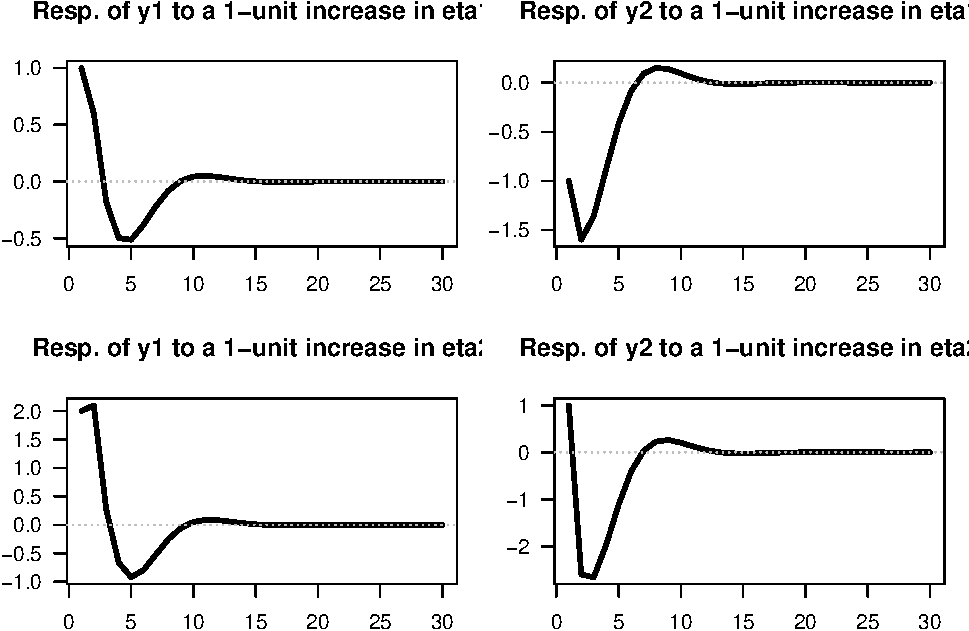
\includegraphics[width=0.95\linewidth]{TimeSeries_files/figure-latex/simVAR-1} \caption{Impulse response functions (SVARMA(1,1) specified above).}\label{fig:simVAR}
\end{figure}

\end{example}

\hypertarget{covariance-stationary-varma-models}{%
\section{Covariance-stationary VARMA models}\label{covariance-stationary-varma-models}}

Let's come back to the infinite MA case (Eq. \eqref{eq:InfMA}):
\[
y_t = \mu + \sum_{h=0}^\infty \Psi_{h} \eta_{t-h}.
\]
For \(y_t\) to be covariance-stationary (and ergodic for the mean), it has to be the case that
\begin{equation}
\sum_{i=0}^\infty \|\Psi_i\| < \infty,\label{eq:condiInfiniteMA}
\end{equation}
where \(\|A\|\) denotes a norm of the matrix \(A\) (e.g.~\(\|A\|=\sqrt{tr(AA')}\)). This notably implies that if \(y_t\) is stationary (and ergodic for the mean), then \(\|\Psi_h\|\rightarrow 0\) when \(h\) gets large.

What should be satisfied by \(\Phi_k\)'s and \(\Theta_k\)'s for a VARMA-based process (Eq. \eqref{eq:yVARMA}) to be stationary? The conditions will be similar to that we have in the univariate case. Let us introduce the following notations:
\begin{eqnarray}
y_t &=& c + \underbrace{\Phi_1 y_{t-1} + \dots +\Phi_p y_{t-p}}_{\color{blue}{\mbox{AR component}}} +  \label{eq:VARMA2}\\
&&\underbrace{B \eta_t - \Theta_1 B \eta_{t-1} - \dots - \Theta_q B \eta_{t-q}}_{\color{red}{\mbox{MA component}}} \nonumber\\
&\Leftrightarrow& \underbrace{ \color{blue}{(I - \Phi_1 L - \dots - \Phi_p L^p)}}_{= \color{blue}{\Phi(L)}}y_t = c +  \underbrace{ \color{red}{(I - \Theta_1 L - \ldots - \Theta_q L^q)}}_{=\color{red}{\Theta(L)}} B \eta_{t}. \nonumber
\end{eqnarray}

Process \(y_t\) is stationary iff the roots of \(\det(\Phi(z))=0\) are strictly outside the unit circle or, equivalently, iff the eigenvalues of
\begin{equation}
\Phi = \left[\begin{array}{cccc}
\Phi_{1} & \Phi_{2} & \cdots & \Phi_{p}\\
I & 0 & \cdots & 0\\
0 & \ddots & 0 & 0\\
0 & 0 & I & 0\end{array}\right]\label{eq:matrixPHI}
\end{equation}
lie strictly within the unit circle. Hence, as is the case for univariate processes, the covariance-stationarity of a VARMA model depends only on the specification of its AR part.

Let's derive the first two unconditional moments of a (covariance-stationary) VARMA process.

Eq. \eqref{eq:VARMA2} gives \(\mathbb{E}(\Phi(L)y_t)=c\), therefore \(\Phi(1)\mathbb{E}(y_t)=c\), or
\[
\mathbb{E}(y_t) = (I - \Phi_1 - \dots - \Phi_p)^{-1}c.
\]
The autocovariances of \(y_t\) can be deduced from the infinite MA representation (Eq. \eqref{eq:InfMA}). We have:
\[
\gamma_j \equiv \mathbb{C}ov(y_t,y_{t-j}) = \sum_{i=j}^\infty \Psi_i \Psi_{i-j}'.
\]
(This infinite sum exists as soon as Eq. \eqref{eq:condiInfiniteMA} is satisfied.)

Conditional means and autocovariances can also be deduced from Eq. \eqref{eq:InfMA}. For \(0 \le h\) and \(0 \le h_1 \le h_2\):
\begin{eqnarray*}
\mathbb{E}_t(y_{t+h}) &=& \mu + \sum_{k=0}^\infty \Psi_{k+h} \eta_{t-k} \\
\mathbb{C}ov_t(y_{t+1+h_1},y_{t+1+h_2}) &=& \sum_{k=0}^{h_1} \Psi_{k}\Psi_{k+h_2-h_1}'.
\end{eqnarray*}

The previous formula implies in particular that the forecasting error \(y_{t+h} - \mathbb{E}_t(y_{t+h})\) has a variance equal to:
\[
\mathbb{V}ar_t(y_{t+1+h}) = \sum_{k=0}^{h} \Psi_{k}\Psi_{k}'.
\]
Because the \(\eta_t\) are mutually and serially independent (and therefore uncorrelated), we have:
\[
\mathbb{V}ar(\Psi_k \eta_{t-k}) = \mathbb{V}ar\left(\sum_{i=1}^n \psi_{k,i} \eta_{i,t-k}\right)  = \sum_{i=1}^n \psi_{k,i}\psi_{k,i}',
\]
where \(\psi_{k,i}\) denotes the \(i^{th}\) column of \(\Psi_k\). This suggests the following decomposition of the variance of the forecast error (called \textbf{variance decomposition}):
\[
\mathbb{V}ar_t(y_{t+1+h}) = \sum_{i=1}^n \underbrace{\sum_{k=0}^{h}  \psi_{k,i}\psi_{k,i}'.}_{\mbox{Contribution of $\eta_{i,t}$}}
\]

Let us now turn to the estimation of VAR models. Note that if there is an MA component (i.e., if we consider a VARMA model), then OLS regressions yield biased estimates (even for asymptotically large samples). Assume for instance that \(y_t\) follows a VARMA(1,1) model:
\[
y_{i,t} = \phi_i y_{t-1} + \varepsilon_{i,t},
\]
where \(\phi_i\) is the \(i^{th}\) row of \(\Phi_1\), and where \(\varepsilon_{i,t}\) is a linear combination of \(\eta_t\) and \(\eta_{t-1}\). Since \(y_{t-1}\) (the regressor) is correlated to \(\eta_{t-1}\), it is also correlated to \(\varepsilon_{i,t}\). The OLS regression of \(y_{i,t}\) on \(y_{t-1}\) yields a biased estimator of \(\phi_i\) (see Figure \ref{fig:simulARMAbiased}). Hence, SVARMA models cannot be consistently estimated by simple OLS regressions (contrary to VAR models, as we will see in the next section); instrumental-variable approaches can be employed to estimate SVARMA models (using past values of \(y_t\) as instruments, see, e.g., \citet{Gourieroux_Monfort_Renne_2020}).

\begin{Shaded}
\begin{Highlighting}[]
\NormalTok{N }\OtherTok{\textless{}{-}} \DecValTok{1000} \CommentTok{\# number of replications}
\NormalTok{T }\OtherTok{\textless{}{-}} \DecValTok{100} \CommentTok{\# sample length}
\NormalTok{phi }\OtherTok{\textless{}{-}}\NormalTok{ .}\DecValTok{8} \CommentTok{\# autoregressive parameter}
\NormalTok{sigma }\OtherTok{\textless{}{-}} \DecValTok{1}
\FunctionTok{par}\NormalTok{(}\AttributeTok{mfrow=}\FunctionTok{c}\NormalTok{(}\DecValTok{1}\NormalTok{,}\DecValTok{2}\NormalTok{))}
\ControlFlowTok{for}\NormalTok{(theta }\ControlFlowTok{in} \FunctionTok{c}\NormalTok{(}\DecValTok{0}\NormalTok{,}\SpecialCharTok{{-}}\FloatTok{0.4}\NormalTok{))\{}
\NormalTok{  all.y }\OtherTok{\textless{}{-}} \FunctionTok{matrix}\NormalTok{(}\DecValTok{0}\NormalTok{,}\DecValTok{1}\NormalTok{,N)}
\NormalTok{  y     }\OtherTok{\textless{}{-}}\NormalTok{ all.y}
\NormalTok{  eta\_1 }\OtherTok{\textless{}{-}} \FunctionTok{rnorm}\NormalTok{(N)}
  \ControlFlowTok{for}\NormalTok{(t }\ControlFlowTok{in} \DecValTok{1}\SpecialCharTok{:}\NormalTok{(T}\SpecialCharTok{+}\DecValTok{1}\NormalTok{))\{}
\NormalTok{    eta }\OtherTok{\textless{}{-}} \FunctionTok{rnorm}\NormalTok{(N)}
\NormalTok{    y }\OtherTok{\textless{}{-}}\NormalTok{ phi }\SpecialCharTok{*}\NormalTok{ y }\SpecialCharTok{+}\NormalTok{ sigma }\SpecialCharTok{*}\NormalTok{ eta }\SpecialCharTok{+}\NormalTok{ theta }\SpecialCharTok{*}\NormalTok{ sigma }\SpecialCharTok{*}\NormalTok{ eta\_1}
\NormalTok{    all.y }\OtherTok{\textless{}{-}} \FunctionTok{rbind}\NormalTok{(all.y,y)}
\NormalTok{    eta\_1 }\OtherTok{\textless{}{-}}\NormalTok{ eta\}}
\NormalTok{  all.y\_1 }\OtherTok{\textless{}{-}}\NormalTok{ all.y[}\DecValTok{1}\SpecialCharTok{:}\NormalTok{T,]}
\NormalTok{  all.y   }\OtherTok{\textless{}{-}}\NormalTok{ all.y[}\DecValTok{2}\SpecialCharTok{:}\NormalTok{(T}\SpecialCharTok{+}\DecValTok{1}\NormalTok{),]}
\NormalTok{  XX\_1 }\OtherTok{\textless{}{-}} \DecValTok{1}\SpecialCharTok{/}\FunctionTok{apply}\NormalTok{(all.y\_1 }\SpecialCharTok{*}\NormalTok{ all.y\_1,}\DecValTok{2}\NormalTok{,sum)}
\NormalTok{  XY   }\OtherTok{\textless{}{-}} \FunctionTok{apply}\NormalTok{(all.y\_1 }\SpecialCharTok{*}\NormalTok{ all.y,}\DecValTok{2}\NormalTok{,sum)}
\NormalTok{  phi.est.OLS }\OtherTok{\textless{}{-}}\NormalTok{ XX\_1 }\SpecialCharTok{*}\NormalTok{ XY}
  \FunctionTok{plot}\NormalTok{(}\FunctionTok{density}\NormalTok{(phi.est.OLS),}\AttributeTok{xlab=}\StringTok{"OLS estimate of phi"}\NormalTok{,}\AttributeTok{ylab=}\StringTok{""}\NormalTok{,}
       \AttributeTok{main=}\FunctionTok{paste}\NormalTok{(}\StringTok{"theta = "}\NormalTok{,theta,}\AttributeTok{sep=}\StringTok{""}\NormalTok{))}
  \FunctionTok{abline}\NormalTok{(}\AttributeTok{v=}\NormalTok{phi,}\AttributeTok{col=}\StringTok{"red"}\NormalTok{,}\AttributeTok{lwd=}\DecValTok{2}\NormalTok{)\}}
\end{Highlighting}
\end{Shaded}

\begin{figure}
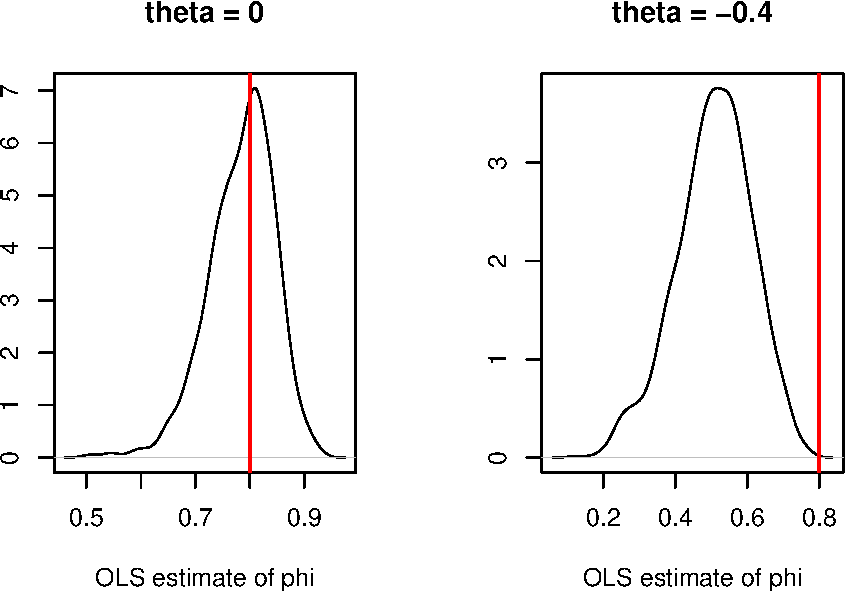
\includegraphics[width=0.95\linewidth]{TimeSeries_files/figure-latex/simulARMAbiased-1} \caption{Illustration of the bias obtained when estimating the auto-regressive parameters of an ARMA process by (standard) OLS.}\label{fig:simulARMAbiased}
\end{figure}

\hypertarget{estimVAR}{%
\section{VAR estimation}\label{estimVAR}}

This section discusses the estimation of VAR models. Eq. \eqref{eq:yVAR} can be written:
\[
y_{t}=c+\Phi(L)y_{t-1}+\varepsilon_{t},
\]
with \(\Phi(L) = \Phi_1 + \Phi_2 L + \dots + \Phi_p L^{p-1}\).

Consequently:
\[
y_{t}\mid y_{t-1},y_{t-2},\ldots,y_{-p+1}\sim \mathcal{N}(c+\Phi_{1}y_{t-1}+\ldots\Phi_{p}y_{t-p},\Omega).
\]

Using \citet{Hamilton_1994}'s notations, denote with \(\Pi\) the matrix \(\left[\begin{array}{ccccc} c & \Phi_{1} & \Phi_{2} & \ldots & \Phi_{p}\end{array}\right]'\) and with \(x_{t}\) the vector \(\left[\begin{array}{ccccc} 1 & y'_{t-1} & y'_{t-2} & \ldots & y'_{t-p}\end{array}\right]'\), we have:
\begin{equation}
y_{t}= \Pi'x_{t} + \varepsilon_{t}. \label{eq:PIVAR}
\end{equation}
The previous representation is convenient to discuss the estimation of the VAR model, as parameters are gathered in two matrices only: \(\Pi\) and \(\Omega\).

Let us start with the case where the shocks are Gaussian.

\begin{proposition}[MLE of a Gaussian VAR]
\protect\hypertarget{prp:estimVARGaussian}{}\label{prp:estimVARGaussian}If \(y_t\) follows a VAR(p) (see Definition \ref{def:SVAR}), and if \(\varepsilon_t \sim \,i.i.d.\,\mathcal{N}(0,\Omega)\), then the ML estimate of \(\Pi\), denoted by \(\hat{\Pi}\) (see Eq. \eqref{eq:PIVAR}), is given by
\begin{equation}
\hat{\Pi}=\left[\sum_{t=1}^{T}x_{t}x'_{t}\right]^{-1}\left[\sum_{t=1}^{T}y_{t}'x_{t}\right]= (\mathbf{X}'\mathbf{X})^{-1}\mathbf{X}'\mathbf{y},\label{eq:Pi}
\end{equation}
where \(\mathbf{X}\) is the \(T \times (1+np)\) matrix whose \(t^{th}\) row is \(x_t\) and where \(\mathbf{y}\) is the \(T \times n\) matrix whose \(t^{th}\) row is \(y_{t}'\).

That is, the \(i^{th}\) column of \(\hat{\Pi}\) (\(b_i\), say) is the OLS estimate of \(\beta_i\), where:
\begin{equation}
y_{i,t} = \beta_i'x_t + \varepsilon_{i,t},\label{eq:betayx}
\end{equation}
(i.e., \(\beta_i' = [c_i,\phi_{i,1}',\dots,\phi_{i,p}']'\)).

The ML estimate of \(\Omega\), denoted by \(\hat{\Omega}\), coincides with the sample covariance matrix of the \(n\) series of the OLS residuals in Eq. \eqref{eq:betayx}, i.e.:
\begin{equation}
\hat{\Omega} = \frac{1}{T} \sum_{i=1}^T \hat{\varepsilon}_t\hat{\varepsilon}_t',\quad\mbox{with } \hat{\varepsilon}_t= y_t - \hat{\Pi}'x_t.
\end{equation}

The asymptotic distributions of these estimators are the ones resulting from standard OLS formula.
\end{proposition}

\begin{proof}
See Appendix \ref{AppendixProof}.
\end{proof}

As stated by Proposition \ref{prp:OLSVAR}, when the shocks are not Gaussian, then the OLS regressions still provide consistent estimates of the model parameters. However, since \(x_t\) correlates to \(\varepsilon_s\) for \(s<t\), the OLS estimator \(\mathbf{b}_i\) of \(\boldsymbol\beta_i\) is biased in small sample. (That is also the case for the ML estimator.) Indeed, denoting by \(\boldsymbol\varepsilon_i\) the \(T \times 1\) vector of \(\varepsilon_{i,t}\)'s, and using the notations of \(b_i\) and \(\beta_i\) introduced in Proposition \ref{prp:estimVARGaussian}, we have:
\begin{equation}
\mathbf{b}_i = \beta_i + (\mathbf{X}'\mathbf{X})^{-1}\mathbf{X}'\boldsymbol\varepsilon_i.\label{eq:olsar1}
\end{equation}
We have non-zero correlation between \(x_t\) and \(\varepsilon_{i,s}\) for \(s<t\) and, therefore, \(\mathbb{E}[(\mathbf{X}'\mathbf{X})^{-1}\mathbf{X}'\boldsymbol\varepsilon_i] \ne 0\).

However, when \(y_t\) is covariance stationary, then \(\frac{1}{n}\mathbf{X}'\mathbf{X}\) converges to a positive definite matrix \(\mathbf{Q}\), and \(\frac{1}{n}X'\boldsymbol\varepsilon_i\) converges to 0. Hence \(\mathbf{b}_i \overset{p}{\rightarrow} \beta_i\). More precisely:

\begin{proposition}[Asymptotic distribution of the OLS estimate of $\beta_i$]
\protect\hypertarget{prp:OLSVAR}{}\label{prp:OLSVAR}If \(y_t\) follows a VAR model, as defined in Definition \ref{def:SVAR}, we have:
\[
\sqrt{T}(\mathbf{b}_i-\beta_i) =  \underbrace{\left[\frac{1}{T}\sum_{t=p}^T x_t x_t' \right]^{-1}}_{\overset{p}{\rightarrow} \mathbf{Q}^{-1}}
\underbrace{\sqrt{T} \left[\frac{1}{T}\sum_{t=1}^T x_t\varepsilon_{i,t} \right]}_{\overset{d}{\rightarrow} \mathcal{N}(0,\sigma_i^2\mathbf{Q})},
\]
where \(\sigma_i = \mathbb{V}ar(\varepsilon_{i,t})\) and where \(\mathbf{Q} = \mbox{plim }\frac{1}{T}\sum_{t=p}^T x_t x_t'\) is given by:
\begin{equation}
\mathbf{Q} = \left[
\begin{array}{ccccc}
1 & \mu' &\mu' & \dots & \mu' \\
\mu & \gamma_0 + \mu\mu' & \gamma_1 + \mu\mu' & \dots & \gamma_{p-1} + \mu\mu'\\
\mu & \gamma_1 + \mu\mu' & \gamma_0 + \mu\mu' & \dots & \gamma_{p-2} + \mu\mu'\\
\vdots &\vdots &\vdots &\dots &\vdots \\
\mu & \gamma_{p-1} + \mu\mu' & \gamma_{p-2} + \mu\mu' & \dots & \gamma_{0} + \mu\mu'
\end{array}
\right].\label{eq:Qols}
\end{equation}
\end{proposition}

\begin{proof}
See Appendix \ref{AppendixProof}.
\end{proof}

The following proposition extends the previous proposition and includes covariances between different \(\beta_i\)'s as well as the asymptotic distribution of the ML estimates of \(\Omega\).

\begin{proposition}[Asymptotic distribution of the OLS estimates]
\protect\hypertarget{prp:OLSVAR2}{}\label{prp:OLSVAR2}If \(y_t\) follows a VAR model, as defined in Definition \ref{def:SVAR}, we have:
\begin{equation}
\sqrt{T}\left[
\begin{array}{c}
vec(\hat\Pi - \Pi)\\
vec(\hat\Omega - \Omega)
\end{array}
\right]
\sim \mathcal{N}\left(0,
\left[
\begin{array}{cc}
\Omega \otimes \mathbf{Q}^{-1} & 0\\
0 & \Sigma_{22}
\end{array}
\right]\right),\label{eq:asymptPi}
\end{equation}
where the component of \(\Sigma_{22}\) corresponding to the covariance between \(\hat\sigma_{i,j}\) and \(\hat\sigma_{k,l}\) (for \(i,j,l,m \in \{1,\dots,n\}^4\)) is equal to \(\sigma_{i,l}\sigma_{j,m}+\sigma_{i,m}\sigma_{j,l}\).
\end{proposition}

\begin{proof}
See \citet{Hamilton_1994}, Appendix of Chapter 11.
\end{proof}

In practice, to use the previous proposition (for instance to implement Monte-Carlo simulations, see Section \ref{MonteCarlo}), \(\Omega\) is replaced with \(\hat{\Omega}\), \(\mathbf{Q}\) is replaced with \(\hat{\mathbf{Q}} = \frac{1}{T}\sum_{t=p}^T x_t x_t'\) and \(\Sigma\) with the matrix whose components are of the form \(\hat\sigma_{i,l}\hat\sigma_{j,m}+\hat\sigma_{i,m}\hat\sigma_{j,l}\), where the \(\hat\sigma_{i,l}\)'s are the components of \(\hat\Omega\).

The simplicity of the VAR framework and the tractability of its MLE open the way to convenient econometric testing. Let's illustrate this with the likelihood ratio test.\footnote{We implement a likelihood ratio test when we want to test whether a restricted version of a wider model is acceptable. For that, we maximize the restricted and unrestricted log-likelihood functions. Assume the respective maximum values are \(\log \mathcal{L}_0\) (for the restricted model, called Model 0) and \(\log \mathcal{L}_1\) (unrestricted model, Model 1). Under the null hypothesis (the restricted model is the true one), we have \(2(\log \mathcal{L}_1 - \log \mathcal{L}_0) \sim \chi^2(r)\), where \(r\) is the number of restrictions imposed on Model 0. (Note that we necessarily have \(\log \mathcal{L}_0 < \log \mathcal{L}_1\).)} The maximum value achieved by the MLE is
\[
\log\mathcal{L}(Y_{T};\hat{\Pi},\hat{\Omega}) = -\frac{Tn}{2}\log(2\pi)+\frac{T}{2}\log\left|\hat{\Omega}^{-1}\right| -\frac{1}{2}\sum_{t=1}^{T}\left[\hat{\varepsilon}_{t}'\hat{\Omega}^{-1}\hat{\varepsilon}_{t}\right].
\]
The last term is:
\begin{eqnarray*}
\sum_{t=1}^{T}\hat{\varepsilon}_{t}'\hat{\Omega}^{-1}\hat{\varepsilon}_{t} &=& \mbox{Tr}\left[\sum_{t=1}^{T}\hat{\varepsilon}_{t}'\hat{\Omega}^{-1}\hat{\varepsilon}_{t}\right] = \mbox{Tr}\left[\sum_{t=1}^{T}\hat{\Omega}^{-1}\hat{\varepsilon}_{t}\hat{\varepsilon}_{t}'\right]\\
&=&\mbox{Tr}\left[\hat{\Omega}^{-1}\sum_{t=1}^{T}\hat{\varepsilon}_{t}\hat{\varepsilon}_{t}'\right] = \mbox{Tr}\left[\hat{\Omega}^{-1}\left(T\hat{\Omega}\right)\right]=Tn.
\end{eqnarray*}
Therefore, the optimized log-likelihood is simply obtained by:
\begin{equation}
\log\mathcal{L}(Y_{T};\hat{\Pi},\hat{\Omega})=-(Tn/2)\log(2\pi)+(T/2)\log\left|\hat{\Omega}^{-1}\right|-Tn/2.\label{eq:optimzedLogL}
\end{equation}

Assume that we want to test the null hypothesis that a set of variables follows a VAR(\(p_{0}\)) against the alternative specification of \(p_{1}\) (\(>p_{0}\)). Let us denote by \(\hat{L}_{0}\) and \(\hat{L}_{1}\) the maximum log-likelihoods obtained with \(p_{0}\) and \(p_{1}\) lags, respectively. Under the null hypothesis (\(H_0\): \(p=p_0\)), we have:
\begin{eqnarray*}
2\left(\hat{L}_{1}-\hat{L}_{0}\right)&=&T\left(\log\left|\hat{\Omega}_{1}^{-1}\right|-\log\left|\hat{\Omega}_{0}^{-1}\right|\right)  \sim \chi^2(n^{2}(p_{1}-p_{0})).
\end{eqnarray*}

What precedes can be used to help determine the appropriate number of lags to use in the specification. In a VAR, using too many lags consumes numerous degrees of freedom: with \(p\) lags, each of the \(n\) equations in the VAR contains \(n\times p\) coefficients plus the intercept term. Adding lags improve in-sample fit, but is likely to result in over-parameterization and affect the \textbf{out-of-sample} prediction performance.

To select appropriate lag length, \textbf{selection criteria} are often used. In the context of VAR models, using Eq. \eqref{eq:optimzedLogL} (Gaussian case), we have for instance:
\begin{eqnarray*}
AIC & = & cst + \log\left|\hat{\Omega}\right|+\frac{2}{T}N\\
BIC & = & cst + \log\left|\hat{\Omega}\right|+\frac{\log T}{T}N,
\end{eqnarray*}
where \(N=p \times n^{2}\).

\begin{Shaded}
\begin{Highlighting}[]
\FunctionTok{library}\NormalTok{(vars);}\FunctionTok{library}\NormalTok{(AEC)}
\NormalTok{data }\OtherTok{\textless{}{-}}\NormalTok{ US3var[,}\FunctionTok{c}\NormalTok{(}\StringTok{"y.gdp.gap"}\NormalTok{,}\StringTok{"infl"}\NormalTok{)]}
\FunctionTok{VARselect}\NormalTok{(data,}\AttributeTok{lag.max =} \DecValTok{6}\NormalTok{)}
\end{Highlighting}
\end{Shaded}

\begin{verbatim}
## $selection
## AIC(n)  HQ(n)  SC(n) FPE(n) 
##      3      3      2      3 
## 
## $criteria
##                 1          2          3          4          5           6
## AIC(n) -0.3394120 -0.4835525 -0.5328327 -0.5210835 -0.5141079 -0.49112812
## HQ(n)  -0.3017869 -0.4208439 -0.4450407 -0.4082080 -0.3761491 -0.32808581
## SC(n)  -0.2462608 -0.3283005 -0.3154798 -0.2416298 -0.1725534 -0.08747275
## FPE(n)  0.7121914  0.6165990  0.5869659  0.5939325  0.5981364  0.61210908
\end{verbatim}

\begin{Shaded}
\begin{Highlighting}[]
\NormalTok{estimated.var }\OtherTok{\textless{}{-}} \FunctionTok{VAR}\NormalTok{(data,}\AttributeTok{p=}\DecValTok{3}\NormalTok{)}
\CommentTok{\#print(estimated.var$varresult)}
\NormalTok{Phi }\OtherTok{\textless{}{-}} \FunctionTok{Acoef}\NormalTok{(estimated.var)}
\NormalTok{PHI }\OtherTok{\textless{}{-}} \FunctionTok{make.PHI}\NormalTok{(Phi) }\CommentTok{\# autoregressive matrix of companion form.}
\FunctionTok{print}\NormalTok{(}\FunctionTok{abs}\NormalTok{(}\FunctionTok{eigen}\NormalTok{(PHI)}\SpecialCharTok{$}\NormalTok{values)) }\CommentTok{\# check stationarity}
\end{Highlighting}
\end{Shaded}

\begin{verbatim}
## [1] 0.9114892 0.9114892 0.6319554 0.4759403 0.4759403 0.3246995
\end{verbatim}

\hypertarget{BlockGranger}{%
\section{Block exogeneity and Granger causality}\label{BlockGranger}}

\hypertarget{block-exogeneity}{%
\subsection{Block exogeneity}\label{block-exogeneity}}

Let's decompose \(y_t\) into two subvectors \(y^{(1)}_{t}\) (\(n_1 \times 1\)) and \(y^{(2)}_{t}\) (\(n_2 \times 1\)), with \(y_t' = [{y^{(1)}_{t}}',{y^{(2)}_{t}}']\) (and therefore \(n=n_1 +n_2\)), such that:
\[
\left[
\begin{array}{c}
y^{(1)}_{t}\\
y^{(2)}_{t}
\end{array}
\right] = \left[
\begin{array}{cc}
\Phi^{(1,1)} & \Phi^{(1,2)}\\
\Phi^{(2,1)} & \Phi^{(2,2)}
\end{array}
\right]
\left[
\begin{array}{c}
y^{(1)}_{t-1}\\
y^{(2)}_{t-1}
\end{array}
\right] + \varepsilon_t.
\]
Using, e.g., a likelihood ratio test, one can easily test for block exogeneity of \(y_t^{(2)}\) (say). The null assumption can be expressed as \(\Phi^{(2,1)}=0\).

\hypertarget{granger-causality}{%
\subsection{Granger Causality}\label{granger-causality}}

\citet{Granger_1969} developed a method to explore \textbf{causal relationships} among variables. The approach consists in determining whether the past values of \(y_{1,t}\) can help explain the current \(y_{2,t}\) (beyond the information already included in the past values of \(y_{2,t}\)).

Formally, let us denote three information sets:
\begin{eqnarray*}
\mathcal{I}_{1,t} & = & \left\{ y_{1,t},y_{1,t-1},\ldots\right\} \\
\mathcal{I}_{2,t} & = & \left\{ y_{2,t},y_{2,t-1},\ldots\right\} \\
\mathcal{I}_{t} & = & \left\{ y_{1,t},y_{1,t-1},\ldots y_{2,t},y_{2,t-1},\ldots\right\}.
\end{eqnarray*}
We say that \(y_{1,t}\) Granger-causes \(y_{2,t}\) if
\[
\mathbb{E}\left[y_{2,t}\mid \mathcal{I}_{2,t-1}\right]\neq \mathbb{E}\left[y_{2,t}\mid \mathcal{I}_{t-1}\right].
\]

To get the intuition behind the testing procedure, consider the following
bivariate VAR(\(p\)) process:
\begin{eqnarray*}
y_{1,t} & = & c_1+\Sigma_{i=1}^{p}\Phi_i^{(11)}y_{1,t-i}+\Sigma_{i=1}^{p}\Phi_i^{(12)}y_{2,t-i}+\varepsilon_{1,t}\\
y_{2,t} & = & c_2+\Sigma_{i=1}^{p}\Phi_i^{(21)}y_{1,t-i}+\Sigma_{i=1}^{p}\Phi_i^{(22)}y_{2,t-i}+\varepsilon_{2,t},
\end{eqnarray*}
where \(\Phi_k^{(ij)}\) denotes the element \((i,j)\) of \(\Phi_k\). Then, \(y_{1,t}\) is said not to Granger-cause \(y_{2,t}\) if
\[
\Phi_1^{(21)}=\Phi_2^{(21)}=\ldots=\Phi_p^{(21)}=0.
\]
The null and alternative hypotheses therefore are:
\[
\begin{cases}
H_{0}: & \Phi_1^{(21)}=\Phi_2^{(21)}=\ldots=\Phi_p^{(21)}=0\\
H_{1}: & \Phi_1^{(21)}\neq0\mbox{ or }\Phi_2^{(21)}\neq0\mbox{ or}\ldots\Phi_p^{(21)}\neq0.\end{cases}
\]
Loosely speaking, we reject \(H_{0}\) if some of the coefficients on the lagged \(y_{1,t}\)'s are statistically significant. Formally, this can be tested using the \(F\)-test or asymptotic chi-square test. The \(F\)-statistic is
\[
F=\frac{(RSS-USS)/p}{USS/(T-2p-1)},
\]
where RSS is the Restricted sum of squared residuals and USS is the Unrestricted sum of squared residuals. Under \(H_{0}\), the \(F\)-statistic is distributed as \(\mathcal{F}(p,T-2p-1)\) (See Table \ref{tab:Fstat}).\footnote{We have \(pF\underset{T \rightarrow \infty}{\rightarrow}\chi^{2}(p)\).}

According to the following lines of code, the output gap Granger-causes inflation, but the reverse is not true:

\begin{Shaded}
\begin{Highlighting}[]
\FunctionTok{grangertest}\NormalTok{(US3var[,}\FunctionTok{c}\NormalTok{(}\StringTok{"y.gdp.gap"}\NormalTok{,}\StringTok{"infl"}\NormalTok{)],}\AttributeTok{order=}\DecValTok{3}\NormalTok{)}
\end{Highlighting}
\end{Shaded}

\begin{verbatim}
## Granger causality test
## 
## Model 1: infl ~ Lags(infl, 1:3) + Lags(y.gdp.gap, 1:3)
## Model 2: infl ~ Lags(infl, 1:3)
##   Res.Df Df      F   Pr(>F)   
## 1    214                      
## 2    217 -3 3.9761 0.008745 **
## ---
## Signif. codes:  0 '***' 0.001 '**' 0.01 '*' 0.05 '.' 0.1 ' ' 1
\end{verbatim}

\begin{Shaded}
\begin{Highlighting}[]
\FunctionTok{grangertest}\NormalTok{(US3var[,}\FunctionTok{c}\NormalTok{(}\StringTok{"infl"}\NormalTok{,}\StringTok{"y.gdp.gap"}\NormalTok{)],}\AttributeTok{order=}\DecValTok{3}\NormalTok{)}
\end{Highlighting}
\end{Shaded}

\begin{verbatim}
## Granger causality test
## 
## Model 1: y.gdp.gap ~ Lags(y.gdp.gap, 1:3) + Lags(infl, 1:3)
## Model 2: y.gdp.gap ~ Lags(y.gdp.gap, 1:3)
##   Res.Df Df      F Pr(>F)
## 1    214                 
## 2    217 -3 1.5451 0.2038
\end{verbatim}

\hypertarget{identifStruct}{%
\section{Standard identification techniques}\label{identifStruct}}

\hypertarget{IdentifPbm}{%
\subsection{The identification problem}\label{IdentifPbm}}

In Section \ref{estimVAR}, we have seen how to estimate \(\mathbb{V}ar(\varepsilon_t) =\Omega\) and the \(\Phi_k\) matrices in the context of a VAR model. But the IRFs are functions of \(B\) and of the \(\Phi_k\)'s, not of \(\Omega\) the \(\Phi_k\)'s (see Section \ref{IRFSVARMA}). We have \(\Omega = BB'\), which provides some restrictions on the components of \(B\), but this is not sufficient to fully identify \(B\). Indeed, seen a system of equations whose unknowns are the \(b_{i,j}\)'s (components of \(B\)), the system \(\Omega = BB'\) contains only \(n(n+1)/2\) linearly independent equations. For instance, for \(n=2\):
\begin{eqnarray*}
&&\left[
\begin{array}{cc}
\omega_{11} & \omega_{12} \\
\omega_{12} & \omega_{22}
\end{array}
\right] = \left[
\begin{array}{cc}
b_{11} & b_{12} \\
b_{21} & b_{22}
\end{array}
\right]\left[
\begin{array}{cc}
b_{11} & b_{21} \\
b_{12} & b_{22}
\end{array}
\right]\\
&\Leftrightarrow&\left[
\begin{array}{cc}
\omega_{11} & \omega_{12} \\
\omega_{12} & \omega_{22}
\end{array}
\right] = \left[
\begin{array}{cc}
b_{11}^2+b_{12}^2 & \color{red}{b_{11}b_{21}+b_{12}b_{22}} \\
\color{red}{b_{11}b_{21}+b_{12}b_{22}} & b_{22}^2 + b_{21}^2
\end{array}
\right].
\end{eqnarray*}

We then have 3 linearly independent equations but 4 unknowns. Therefore, \(B\) is not identified based on second-order moments. Additional restrictions are required to identify \(B\). This section covers two standard identification schemes: \textbf{short-run} and \textbf{long-run} restrictions.

\begin{enumerate}
\def\labelenumi{\arabic{enumi}.}
\tightlist
\item
  A \textbf{short-run restriction (SRR)} prevents a structural shock from affecting an endogenous variable contemporaneously.
\end{enumerate}

\begin{itemize}
\tightlist
\item
  It is easy to implement: the appropriate entries of \(B\) are set to 0.
\item
  A particular (popular) case is that of the \textbf{Cholesky, or recursive approach}.
\item
  Examples include \citet{BERNANKE198649}, \citet{Sims_1986}, \citet{Gali_1992}, \citet{RubioRamirez_et_al_2010}.
\end{itemize}

\begin{enumerate}
\def\labelenumi{\arabic{enumi}.}
\setcounter{enumi}{1}
\tightlist
\item
  A \textbf{long-run restriction (LRR)} prevents a structural shock from having a cumulative impact on one of the endogenous variables.
\end{enumerate}

\begin{itemize}
\tightlist
\item
  Additional computations are required to implement this. One needs to compute the cumulative effect of one of the structural shocks \(u_{t}\) on one of the endogenous variable.
\item
  Examples include \citet{Blanchard_Quah_1989}, \citet{Faust_Leeper_1997}, \citet{Gali_1999}, \citet{Erceg_et_al_2005}, \citet{NBERc11177}.
\end{itemize}

The two approaches can be combined (see, e.g., \citet{Gerlach_Smets_1995}).

\hypertarget{a-stylized-example-motivating-short-run-restrictions}{%
\subsection{A stylized example motivating short-run restrictions}\label{a-stylized-example-motivating-short-run-restrictions}}

Let us consider a simple example that could motivate short-run restrictions. Consider the following stylized macro model:
\begin{equation}
\begin{array}{clll}
g_{t}&=& \bar{g}-\lambda(i_{t-1}-\mathbb{E}_{t-1}\pi_{t})+ \underbrace{{\color{blue}\sigma_d \eta_{d,t}}}_{\mbox{demand shock}}& (\mbox{IS curve})\\
\Delta \pi_{t} & = & \beta (g_{t} - \bar{g})+ \underbrace{{\color{blue}\sigma_{\pi} \eta_{\pi,t}}}_{\mbox{cost push shock}} & (\mbox{Phillips curve})\\
i_{t} & = & \rho i_{t-1} + \left[ \gamma_\pi \mathbb{E}_{t}\pi_{t+1}  + \gamma_g (g_{t} - \bar{g}) \right]\\
&& \qquad \qquad+\underbrace{{\color{blue}\sigma_{mp} \eta_{mp,t}}}_{\mbox{Mon. Pol. shock}} & (\mbox{Taylor rule}),
\end{array}\label{eq:systemI}
\end{equation}
where:
\begin{equation}
\eta_t = 
\left[
\begin{array}{c}
\eta_{\pi,t}\\
\eta_{d,t}\\
\eta_{mp,t}
\end{array}
\right]
\sim i.i.d.\,\mathcal{N}(0,I).\label{eq:covU}
\end{equation}

Vector \(\eta_t\) is assumed to be a vector of structural shocks, mutually and serially independent. On date \(t\):

\begin{itemize}
\tightlist
\item
  \(g_t\) is contemporaneously affected by \(\eta_{d,t}\) only;
\item
  \(\pi_t\) is contemporaneously affected by \(\eta_{\pi,t}\) and \(\eta_{d,t}\);
\item
  \(i_t\) is contemporaneously affected by \(\eta_{mp,t}\), \(\eta_{\pi,t}\) and \(\eta_{d,t}\).
\end{itemize}

System \eqref{eq:systemI} could be rewritten as follows:
\begin{equation}
\left[\begin{array}{c}
d_t\\
\pi_t\\
i_t
\end{array}\right]
= \Phi(L)
\left[\begin{array}{c}
d_{t-1}\\
\pi_{t-1}\\
i_{t-1} +
\end{array}\right] +\underbrace{\underbrace{
\left[
\begin{array}{ccc}
0 & \bullet & 0 \\
\bullet & \bullet & 0 \\
\bullet & \bullet & \bullet
\end{array}
\right]}_{=B} \eta_t.}_{=\varepsilon_t}\label{eq:BBBB}
\end{equation}

This is the \textbf{reduced-form} of the model. This representation suggests three additional restrictions on the entries of \(B\); the latter matrix is therefore identified as soon as \(\Omega = BB'\) is known (up to the signs of its columns).

\hypertarget{cholesky-a-specific-short-run-restriction-situation}{%
\subsection{Cholesky: a specific short-run-restriction situation}\label{cholesky-a-specific-short-run-restriction-situation}}

There are particular cases in which some well-known matrix decomposition of \(\Omega=\mathbb{V}ar(\varepsilon_t)\) can be used to easily estimate some specific SVAR. This is the case for the so-called Cholesky decomposition. Consider the following context:

\begin{itemize}
\tightlist
\item
  A first shock (say, \(\eta_{n_1,t}\)) can affect instantaneously
  (i.e., on date \(t\)) only one of the endogenous variable (say, \(y_{n_1,t}\));
\item
  A second shock (say, \(\eta_{n_2,t}\)) can affect instantaneously
  (i.e., on date \(t\)) two endogenous variables, \(y_{n_1,t}\) (the same as before) and \(y_{n_2,t}\);
\item
  \(\dots\)
\end{itemize}

This implies

\begin{enumerate}
\def\labelenumi{\arabic{enumi}.}
\tightlist
\item
  that column \(n_1\) of \(B\) has only 1 non-zero entry (this is the \(n_1^{th}\) entry),
\item
  that column \(n_2\) of \(B\) has 2 non-zero entries (the \(n_1^{th}\) and the \(n_2^{th}\) ones), etc.
\end{enumerate}

Without loss of generality, we can set \(n_1=n\), \(n_2=n-1\), etc. In this context, matrix \(B\) is lower triangular. The Cholesky decomposition of \(\Omega_{\varepsilon}\) then provides an appropriate estimate of \(B\), since this matrix decomposition yields to a lower triangular matrix satisfying:
\[
\Omega_\varepsilon = BB'.
\]

For instance, \citet{DEDOLA20051543} estimate 5 structural VAR models for the US, the UK, Germany, France and Italy to analyse the monetary-policy transmission mechanisms. They estimate SVAR(5) models over the period 1975-1997. The shock-identification scheme is based on Cholesky decompositions, the ordering of the endogenous variables being: the industrial production, the consumer price index, a commodity price index, the short-term rate, monetary aggregate and the effective exchange rate (except for the US). This ordering implies that monetary policy reacts to the shocks affecting the first three variables but that the latter react to monetary policy shocks with a one-period lag only.

The Cholesky approach can be employed when one is interested in one specific structural shock. This is the case, e.g., of \citet{Christiano_Eichenbaum_Evans_1996}. Their identification is based on the following relationship between \(\varepsilon_t\) and \(\eta_t\):
\[
\left[\begin{array}{c}
\boldsymbol\varepsilon_{S,t}\\
\varepsilon_{r,t}\\
\boldsymbol\varepsilon_{F,t}
\end{array}\right] =
\left[\begin{array}{ccc}
B_{SS} & 0 & 0 \\
B_{rS} & B_{rr} & 0 \\
B_{FS} & B_{Fr} & B_{FF}
\end{array}\right]
\left[\begin{array}{c}
\boldsymbol\eta_{S,t}\\
\eta_{r,t}\\
\boldsymbol\eta_{F,t}
\end{array}\right],
\]
where \(S\), \(r\) and \(F\) respectively correspond to \emph{slow-moving variables}, the policy variable (short-term rate) and \emph{fast-moving variables}. While \(\eta_{r,t}\) is scalar, \(\boldsymbol\eta_{S,t}\) and \(\boldsymbol\eta_{F,t}\) may be vectors. The space spanned by \(\boldsymbol\varepsilon_{S,t}\) is the same as that spanned by \(\boldsymbol\eta_{S,t}\). As a result, because \(\varepsilon_{r,t}\) is a linear combination of \(\eta_{r,t}\) and \(\boldsymbol\eta_{S,t}\) (which are \(\perp\)), it comes that the \(B_{rr}\eta_{r,t}\)'s are the (population) residuals in the regression of \(\varepsilon_{r,t}\) on \(\boldsymbol\varepsilon_{S,t}\). Because \(\mathbb{V}ar(\eta_{r,t})=1\), \(B_{rr}\) is given by the square root of the variance of \(B_{rr}\eta_{r,t}\). \(B_{F,r}\) is finally obtained by regressing the components of \(\boldsymbol\varepsilon_{F,t}\) on the estimates of \(\eta_{r,t}\).

An equivalent approach consists in computing the Cholesky decomposition of \(BB'\) and the contemporaneous impacts of the monetary policy shock (on the \(n\) endogenous variables) are the components of the column of \(B\) corresponding to the policy variable.

\begin{Shaded}
\begin{Highlighting}[]
\FunctionTok{library}\NormalTok{(AEC);}\FunctionTok{library}\NormalTok{(vars)}
\FunctionTok{data}\NormalTok{(}\StringTok{"USmonthly"}\NormalTok{)}
\CommentTok{\# Select sample period:}
\NormalTok{First.date }\OtherTok{\textless{}{-}} \StringTok{"1965{-}01{-}01"}\NormalTok{;Last.date }\OtherTok{\textless{}{-}} \StringTok{"1995{-}06{-}01"}
\NormalTok{indic.first }\OtherTok{\textless{}{-}} \FunctionTok{which}\NormalTok{(USmonthly}\SpecialCharTok{$}\NormalTok{DATES}\SpecialCharTok{==}\NormalTok{First.date)}
\NormalTok{indic.last  }\OtherTok{\textless{}{-}} \FunctionTok{which}\NormalTok{(USmonthly}\SpecialCharTok{$}\NormalTok{DATES}\SpecialCharTok{==}\NormalTok{Last.date)}
\NormalTok{USmonthly   }\OtherTok{\textless{}{-}}\NormalTok{ USmonthly[indic.first}\SpecialCharTok{:}\NormalTok{indic.last,]}
\NormalTok{considered.variables }\OtherTok{\textless{}{-}} \FunctionTok{c}\NormalTok{(}\StringTok{"LIP"}\NormalTok{,}\StringTok{"UNEMP"}\NormalTok{,}\StringTok{"LCPI"}\NormalTok{,}\StringTok{"LPCOM"}\NormalTok{,}\StringTok{"FFR"}\NormalTok{,}\StringTok{"NBR"}\NormalTok{,}\StringTok{"TTR"}\NormalTok{,}\StringTok{"M1"}\NormalTok{)}
\NormalTok{y }\OtherTok{\textless{}{-}} \FunctionTok{as.matrix}\NormalTok{(USmonthly[considered.variables])}
\NormalTok{res.svar.ordering }\OtherTok{\textless{}{-}} \FunctionTok{svar.ordering}\NormalTok{(y,}\AttributeTok{p=}\DecValTok{3}\NormalTok{,}
                                   \AttributeTok{posit.of.shock =} \DecValTok{5}\NormalTok{,}
                                   \AttributeTok{nb.periods.IRF =} \DecValTok{20}\NormalTok{,}
                                   \AttributeTok{nb.bootstrap.replications =} \DecValTok{100}\NormalTok{,}
                                   \AttributeTok{confidence.interval =} \FloatTok{0.90}\NormalTok{, }\CommentTok{\# expressed in pp.}
                                   \AttributeTok{indic.plot =} \DecValTok{1} \CommentTok{\# Plots are displayed if = 1.}
\NormalTok{)}
\end{Highlighting}
\end{Shaded}

\begin{figure}
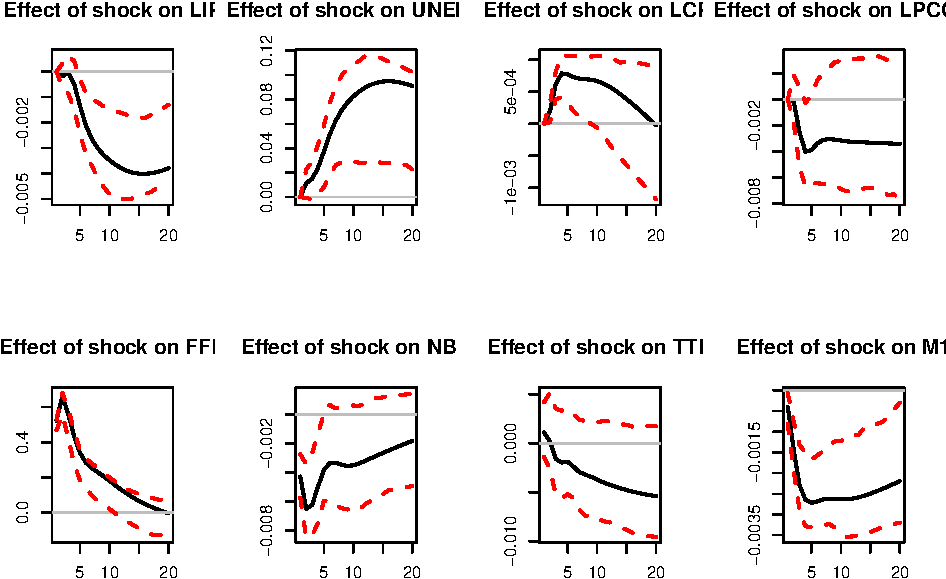
\includegraphics[width=0.95\linewidth]{TimeSeries_files/figure-latex/CEE-1} \caption{Response to a monetary-policy shock. Identification approach of Christiano, Eichenbaum and Evans (1996). Confidence intervals are obtained by boostrapping the estimated VAR model (see inference section).}\label{fig:CEE}
\end{figure}

\hypertarget{long-run-restrictions}{%
\subsection{Long-run restrictions}\label{long-run-restrictions}}

Let us now turn to \textbf{Long-run restrictions}. Such a restriction concerns the long-run influence of a shock on an endogenous variable. Let us consider for instance a structural shock that is assumed to have no ``long-run influence'' on GDP. How to express this? The long-run change in GDP can be expressed as \(GDP_{t+h} - GDP_t\), with \(h\) large. Note further that:
\[
GDP_{t+h} - GDP_t = \Delta GDP_{t+h} +\Delta GDP_{t+h-1} + \dots + \Delta GDP_{t+1}.
\]
Hence, the fact that a given structural shock (\(\eta_{i,t}\), say) has no long-run influence on GDP means that
\[
\lim_{h\rightarrow\infty}\frac{\partial GDP_{t+h}}{\partial \eta_{i,t}} = \lim_{h\rightarrow\infty} \frac{\partial}{\partial \eta_{i,t}}\left(\sum_{k=1}^h \Delta  GDP_{t+k}\right)= 0.
\]

This long-run effect can be formulated as a function of \(B\) and of the matrices \(\Phi_i\) when \(y_t\) (including \(\Delta GDP_t\)) follows a VAR process.

Without loss of generality, we will only consider the VAR(1) case. Indeed, one can always write a VAR(\(p\)) as a VAR(1): for that, stack the last \(p\) values of vector \(y_t\) in vector \(y_{t}^{*}=[y_t',\dots,y_{t-p+1}']'\); Eq. \eqref{eq:yVAR} can then be rewritten in its \textbf{companion form}:
\begin{equation}
y_{t}^{*} =
\underbrace{\left[\begin{array}{c}
c\\
0\\
\vdots\\
0\end{array}\right]}_{=c^*}+
\underbrace{\left[\begin{array}{cccc}
\Phi_{1} & \Phi_{2} & \cdots & \Phi_{p}\\
I & 0 & \cdots & 0\\
0 & \ddots & 0 & 0\\
0 & 0 & I & 0\end{array}\right]}_{=\Phi}
y_{t-1}^{*}+
\underbrace{\left[\begin{array}{c}
\varepsilon_{t}\\
0\\
\vdots\\
0\end{array}\right]}_{\varepsilon_t^*},\label{eq:ystarVAR}
\end{equation}
where matrices \(\Phi\) and \(\Omega^* = \mathbb{V}ar(\varepsilon_t^*)\) are of dimension \(np \times np\); \(\Omega^*\) is filled with zeros, except the \(n\times n\) upper-left block that is equal to \(\Omega = \mathbb{V}ar(\varepsilon_t)\). (Matrix \(\Phi\) had been introduced in Eq. \eqref{eq:matrixPHI}.)

Let us then focus on the VAR(1) case:
\begin{eqnarray*}
y_{t} &=& c+\Phi y_{t-1}+\varepsilon_{t}\\
& = & c+\varepsilon_{t}+\Phi(c+\varepsilon_{t-1})+\ldots+\Phi^{k}(c+\varepsilon_{t-k})+\ldots \\
& = & \mu +\varepsilon_{t}+\Phi\varepsilon_{t-1}+\ldots+\Phi^{k}\varepsilon_{t-k}+\ldots \\
& = & \mu +B\eta_{t}+\Phi B\eta_{t-1}+\ldots+\Phi^{k}B\eta_{t-k}+\ldots,
\end{eqnarray*}
which is the Wold representation of \(y_t\).

The sequence of shocks \(\{\eta_t\}\) determines the sequence \(\{y_t\}\). What if \(\{\eta_t\}\) is replaced with \(\{\tilde{\eta}_t\}\), where \(\tilde{\eta}_t=\eta_t\) if \(t \ne s\) and \(\tilde{\eta}_s=\eta_s + \gamma\)? Assume \(\{\tilde{y}_t\}\) is the associated ``perturbated'' sequence. We have \(\tilde{y}_t = y_t\) if \(t<s\). For \(t \ge s\), the Wold decomposition of \(\{\tilde{y}_t\}\) implies:
\[
\tilde{y}_t = y_t + \Phi^{t-s} B \gamma.
\]
Therefore, the cumulative impact of \(\gamma\) on \(\tilde{y}_t\) will be (for \(t \ge s\)):
\begin{eqnarray}
(\tilde{y}_t - y_t) +  (\tilde{y}_{t-1} - y_{t-1}) + \dots +  (\tilde{y}_s - y_s) &=& \nonumber \\
(Id + \Phi + \Phi^2 + \dots + \Phi^{t-s}) B \gamma.&& \label{eq:cumul}
\end{eqnarray}

Consider a shock on \(\eta_{1,t}\), with a magnitude of \(1\). This shock corresponds to \(\gamma = [1,0,\dots,0]'\). Given Eq. \eqref{eq:cumul}, the long-run cumulative effect of this shock on the endogenous variables is given by:
\[
\underbrace{(Id+\Phi+\ldots+\Phi^{k}+\ldots)}_{=(Id - \Phi)^{-1}}B\left[\begin{array}{c}
1\\
0\\
\vdots\\
0\end{array}\right],
\]
that is the first column of the \(n \times n\) matrix \(\Theta \equiv (Id - \Phi)^{-1}B\).

In this context, consider the following long-run restriction: \emph{``the \(j^{th}\) structural shock has no cumulative impact on the \(i^{th}\) endogenous variable''}. It is equivalent to
\[
\Theta_{ij}=0,
\]
where \(\Theta_{ij}\) is the element \((i,j)\) of \(\Theta\).

\citet{Blanchard_Quah_1989} have implemented such long-run restrictions in a small-scale VAR. Two variables are considered: GDP and unemployment. Consequently, the VAR is affected by two types of shocks. Specifically, authors want to identify \textbf{supply shocks} (that can have a permanent effect on output) and \textbf{demand shocks} (that cannot have a permanent effect on output).\footnote{The motivation of the authors regarding their long-run restrictions can be obtained from a traditional Keynesian view of fluctuations. The authors propose a variant of a model from \citet{Fischer_1977}.
}

\citet{Blanchard_Quah_1989}'s dataset is quarterly, spanning the period from 1950:2 to 1987:4. Their VAR features 8 lags. Here are the data they use:

\begin{Shaded}
\begin{Highlighting}[]
\FunctionTok{library}\NormalTok{(AEC)}
\FunctionTok{data}\NormalTok{(BQ)}
\FunctionTok{par}\NormalTok{(}\AttributeTok{mfrow=}\FunctionTok{c}\NormalTok{(}\DecValTok{1}\NormalTok{,}\DecValTok{2}\NormalTok{))}
\FunctionTok{plot}\NormalTok{(BQ}\SpecialCharTok{$}\NormalTok{Date,BQ}\SpecialCharTok{$}\NormalTok{Dgdp,}\AttributeTok{type=}\StringTok{"l"}\NormalTok{,}\AttributeTok{main=}\StringTok{"GDP quarterly growth rate"}\NormalTok{,}
     \AttributeTok{xlab=}\StringTok{""}\NormalTok{,}\AttributeTok{ylab=}\StringTok{""}\NormalTok{,}\AttributeTok{lwd=}\DecValTok{2}\NormalTok{)}
\FunctionTok{plot}\NormalTok{(BQ}\SpecialCharTok{$}\NormalTok{Date,BQ}\SpecialCharTok{$}\NormalTok{unemp,}\AttributeTok{type=}\StringTok{"l"}\NormalTok{,}\AttributeTok{ylim=}\FunctionTok{c}\NormalTok{(}\SpecialCharTok{{-}}\DecValTok{3}\NormalTok{,}\DecValTok{6}\NormalTok{),}\AttributeTok{main=}\StringTok{"Unemployment rate (gap)"}\NormalTok{,}
     \AttributeTok{xlab=}\StringTok{""}\NormalTok{,}\AttributeTok{ylab=}\StringTok{""}\NormalTok{,}\AttributeTok{lwd=}\DecValTok{2}\NormalTok{)}
\end{Highlighting}
\end{Shaded}

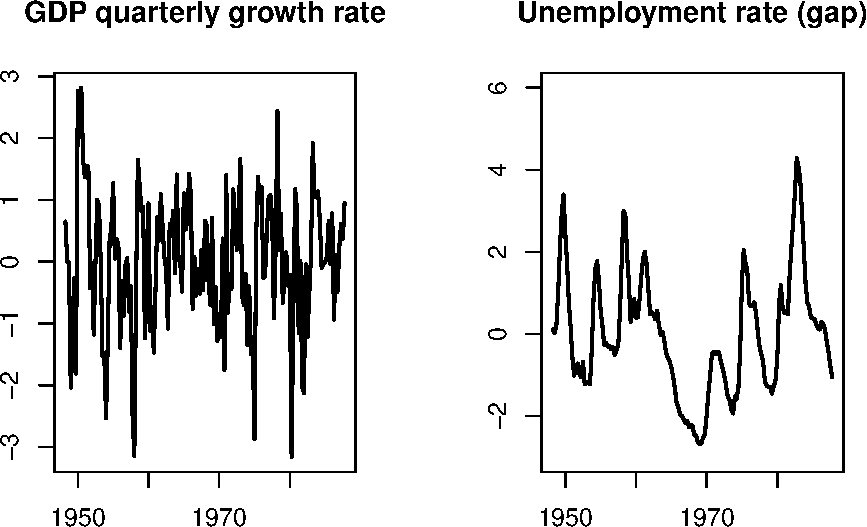
\includegraphics{TimeSeries_files/figure-latex/BQ1-1.pdf}

Estimate a reduced-form VAR(8) model:

\begin{Shaded}
\begin{Highlighting}[]
\FunctionTok{library}\NormalTok{(vars)}
\NormalTok{y }\OtherTok{\textless{}{-}}\NormalTok{ BQ[,}\DecValTok{2}\SpecialCharTok{:}\DecValTok{3}\NormalTok{]}
\NormalTok{est.VAR }\OtherTok{\textless{}{-}} \FunctionTok{VAR}\NormalTok{(y,}\AttributeTok{p=}\DecValTok{8}\NormalTok{)}
\NormalTok{Omega }\OtherTok{\textless{}{-}} \FunctionTok{var}\NormalTok{(}\FunctionTok{residuals}\NormalTok{(est.VAR))}
\end{Highlighting}
\end{Shaded}

Now, let us define a loss function (\texttt{loss}) that is equal to zero if (a) \(BB'=\Omega\) and (b) the element (1,1) of \(\Theta = (Id - \Phi)^{-1} B\) is equal to zero:

\begin{Shaded}
\begin{Highlighting}[]
\CommentTok{\# Compute (Id {-} Phi)\^{}\{{-}1\}:}
\NormalTok{Phi }\OtherTok{\textless{}{-}} \FunctionTok{Acoef}\NormalTok{(est.VAR)}
\NormalTok{PHI }\OtherTok{\textless{}{-}} \FunctionTok{make.PHI}\NormalTok{(Phi)}
\NormalTok{sum.PHI.k }\OtherTok{\textless{}{-}} \FunctionTok{solve}\NormalTok{(}\FunctionTok{diag}\NormalTok{(}\FunctionTok{dim}\NormalTok{(PHI)[}\DecValTok{1}\NormalTok{]) }\SpecialCharTok{{-}}\NormalTok{ PHI)[}\DecValTok{1}\SpecialCharTok{:}\DecValTok{2}\NormalTok{,}\DecValTok{1}\SpecialCharTok{:}\DecValTok{2}\NormalTok{]}
\NormalTok{loss }\OtherTok{\textless{}{-}} \ControlFlowTok{function}\NormalTok{(param)\{}
\NormalTok{  B }\OtherTok{\textless{}{-}} \FunctionTok{matrix}\NormalTok{(param,}\DecValTok{2}\NormalTok{,}\DecValTok{2}\NormalTok{)}
\NormalTok{  X }\OtherTok{\textless{}{-}}\NormalTok{ Omega }\SpecialCharTok{{-}}\NormalTok{ B }\SpecialCharTok{\%*\%} \FunctionTok{t}\NormalTok{(B)}
\NormalTok{  Theta }\OtherTok{\textless{}{-}}\NormalTok{ sum.PHI.k[}\DecValTok{1}\SpecialCharTok{:}\DecValTok{2}\NormalTok{,}\DecValTok{1}\SpecialCharTok{:}\DecValTok{2}\NormalTok{] }\SpecialCharTok{\%*\%}\NormalTok{ B}
\NormalTok{  loss }\OtherTok{\textless{}{-}} \DecValTok{10000} \SpecialCharTok{*}\NormalTok{ ( X[}\DecValTok{1}\NormalTok{,}\DecValTok{1}\NormalTok{]}\SpecialCharTok{\^{}}\DecValTok{2} \SpecialCharTok{+}\NormalTok{ X[}\DecValTok{2}\NormalTok{,}\DecValTok{1}\NormalTok{]}\SpecialCharTok{\^{}}\DecValTok{2} \SpecialCharTok{+}\NormalTok{ X[}\DecValTok{2}\NormalTok{,}\DecValTok{2}\NormalTok{]}\SpecialCharTok{\^{}}\DecValTok{2} \SpecialCharTok{+}\NormalTok{ Theta[}\DecValTok{1}\NormalTok{,}\DecValTok{1}\NormalTok{]}\SpecialCharTok{\^{}}\DecValTok{2}\NormalTok{ )}
  \FunctionTok{return}\NormalTok{(loss)}
\NormalTok{\}}
\NormalTok{res.opt }\OtherTok{\textless{}{-}} \FunctionTok{optim}\NormalTok{(}\FunctionTok{c}\NormalTok{(}\DecValTok{1}\NormalTok{,}\DecValTok{0}\NormalTok{,}\DecValTok{0}\NormalTok{,}\DecValTok{1}\NormalTok{),loss,}\AttributeTok{method=}\StringTok{"BFGS"}\NormalTok{,}\AttributeTok{hessian=}\ConstantTok{FALSE}\NormalTok{)}
\FunctionTok{print}\NormalTok{(res.opt}\SpecialCharTok{$}\NormalTok{par)}
\end{Highlighting}
\end{Shaded}

\begin{verbatim}
## [1]  0.8570358 -0.2396345  0.1541395  0.1921221
\end{verbatim}

(Note: one can use that type of approach, based on a loss function, to mix short- and long-run restrictions.)

Figure \ref{fig:BQ4} displays the resulting IRFs. Note that, for GDP, we cumulate the GDP growth IRF, so as to have the response of the GDP in level.

\begin{Shaded}
\begin{Highlighting}[]
\NormalTok{B.hat }\OtherTok{\textless{}{-}} \FunctionTok{matrix}\NormalTok{(res.opt}\SpecialCharTok{$}\NormalTok{par,}\DecValTok{2}\NormalTok{,}\DecValTok{2}\NormalTok{)}
\FunctionTok{print}\NormalTok{(}\FunctionTok{cbind}\NormalTok{(Omega,B.hat }\SpecialCharTok{\%*\%} \FunctionTok{t}\NormalTok{(B.hat)))}
\end{Highlighting}
\end{Shaded}

\begin{verbatim}
##             Dgdp       unemp                       
## Dgdp   0.7582704 -0.17576173  0.7582694 -0.17576173
## unemp -0.1757617  0.09433658 -0.1757617  0.09433558
\end{verbatim}

\begin{Shaded}
\begin{Highlighting}[]
\NormalTok{nb.sim }\OtherTok{\textless{}{-}} \DecValTok{40}
\FunctionTok{par}\NormalTok{(}\AttributeTok{mfrow=}\FunctionTok{c}\NormalTok{(}\DecValTok{2}\NormalTok{,}\DecValTok{2}\NormalTok{));}\FunctionTok{par}\NormalTok{(}\AttributeTok{plt=}\FunctionTok{c}\NormalTok{(.}\DecValTok{15}\NormalTok{,.}\DecValTok{95}\NormalTok{,.}\DecValTok{15}\NormalTok{,.}\DecValTok{8}\NormalTok{))}
\NormalTok{Y }\OtherTok{\textless{}{-}} \FunctionTok{simul.VAR}\NormalTok{(}\AttributeTok{c=}\FunctionTok{matrix}\NormalTok{(}\DecValTok{0}\NormalTok{,}\DecValTok{2}\NormalTok{,}\DecValTok{1}\NormalTok{),Phi,B.hat,nb.sim,}\AttributeTok{y0.star=}\FunctionTok{rep}\NormalTok{(}\DecValTok{0}\NormalTok{,}\DecValTok{2}\SpecialCharTok{*}\DecValTok{8}\NormalTok{),}
               \AttributeTok{indic.IRF =} \DecValTok{1}\NormalTok{,}\AttributeTok{u.shock =} \FunctionTok{c}\NormalTok{(}\DecValTok{1}\NormalTok{,}\DecValTok{0}\NormalTok{))}
\FunctionTok{plot}\NormalTok{(}\FunctionTok{cumsum}\NormalTok{(Y[,}\DecValTok{1}\NormalTok{]),}\AttributeTok{type=}\StringTok{"l"}\NormalTok{,}\AttributeTok{lwd=}\DecValTok{2}\NormalTok{,}\AttributeTok{xlab=}\StringTok{""}\NormalTok{,}\AttributeTok{ylab=}\StringTok{""}\NormalTok{,}\AttributeTok{main=}\StringTok{"Demand shock on GDP"}\NormalTok{)}
\FunctionTok{plot}\NormalTok{(Y[,}\DecValTok{2}\NormalTok{],}\AttributeTok{type=}\StringTok{"l"}\NormalTok{,}\AttributeTok{lwd=}\DecValTok{2}\NormalTok{,}\AttributeTok{xlab=}\StringTok{""}\NormalTok{,}\AttributeTok{ylab=}\StringTok{""}\NormalTok{,}\AttributeTok{main=}\StringTok{"Demand shock on UNEMP"}\NormalTok{)}
\NormalTok{Y }\OtherTok{\textless{}{-}} \FunctionTok{simul.VAR}\NormalTok{(}\AttributeTok{c=}\FunctionTok{matrix}\NormalTok{(}\DecValTok{0}\NormalTok{,}\DecValTok{2}\NormalTok{,}\DecValTok{1}\NormalTok{),Phi,B.hat,nb.sim,}\AttributeTok{y0.star=}\FunctionTok{rep}\NormalTok{(}\DecValTok{0}\NormalTok{,}\DecValTok{2}\SpecialCharTok{*}\DecValTok{8}\NormalTok{),}
               \AttributeTok{indic.IRF =} \DecValTok{1}\NormalTok{,}\AttributeTok{u.shock =} \FunctionTok{c}\NormalTok{(}\DecValTok{0}\NormalTok{,}\DecValTok{1}\NormalTok{))}
\FunctionTok{plot}\NormalTok{(}\FunctionTok{cumsum}\NormalTok{(Y[,}\DecValTok{1}\NormalTok{]),}\AttributeTok{type=}\StringTok{"l"}\NormalTok{,}\AttributeTok{lwd=}\DecValTok{2}\NormalTok{,}\AttributeTok{xlab=}\StringTok{""}\NormalTok{,}\AttributeTok{ylab=}\StringTok{""}\NormalTok{,}\AttributeTok{main=}\StringTok{"Supply shock on GDP"}\NormalTok{)}
\FunctionTok{plot}\NormalTok{(Y[,}\DecValTok{2}\NormalTok{],}\AttributeTok{type=}\StringTok{"l"}\NormalTok{,}\AttributeTok{lwd=}\DecValTok{2}\NormalTok{,}\AttributeTok{xlab=}\StringTok{""}\NormalTok{,}\AttributeTok{ylab=}\StringTok{""}\NormalTok{,}\AttributeTok{main=}\StringTok{"Supply shock on UNEMP"}\NormalTok{)}
\end{Highlighting}
\end{Shaded}

\begin{figure}
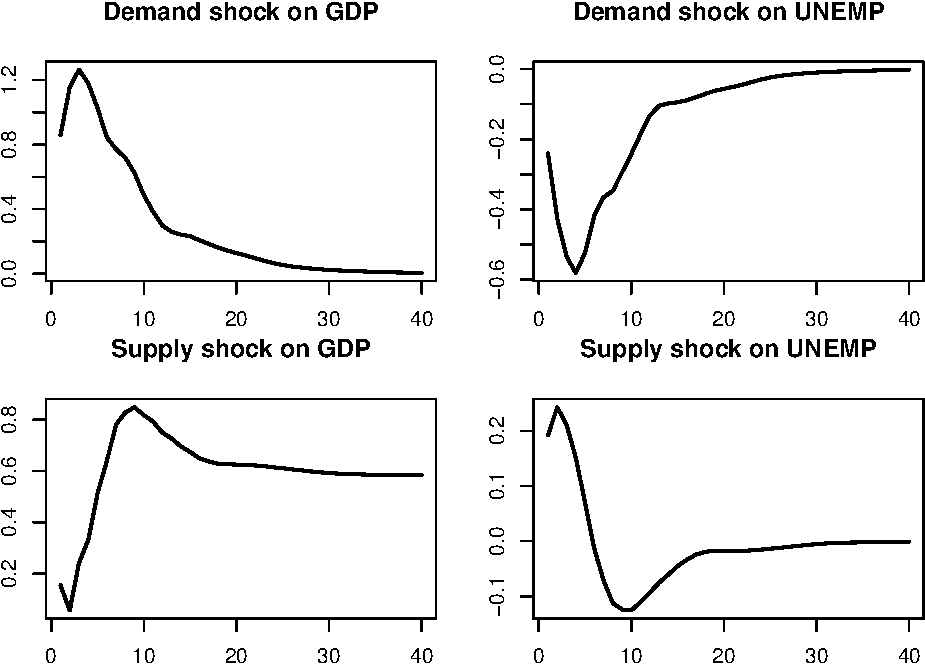
\includegraphics[width=0.95\linewidth]{TimeSeries_files/figure-latex/BQ4-1} \caption{IRF of GDP and unemployment to demand and supply shocks.}\label{fig:BQ4}
\end{figure}

\hypertarget{forecasting}{%
\chapter{Forecasting}\label{forecasting}}

Forecasting has always been an important part of the time series field (\citet{DEGOOIJER2006443}). Macroeconomic forecasts are done in many places: Public Administration (notably Treasuries), Central Banks, International Institutions (e.g.~IMF, OECD), banks, big firms. These institutions are interested in the \textbf{point estimates} (\(\sim\) most likely value) of the variable of interest. They also sometimes need to measure the \textbf{uncertainty} (\(\sim\) dispersion of likely outcomes) associated to the point estimates.\footnote{In its inflation report, the Bank of England displays charts showing the conditional distribution of future inflation, called fan charts. This fan charts show the uncertainty associated with future inflation. See \href{https://www.bankofengland.co.uk/quarterly-bulletin/1998/q1/the-inflation-report-projections-understanding-the-fan-chart}{this page}.}

Forecasts produced by professional forecasters are available on these web pages:

\begin{itemize}
\tightlist
\item
  \href{https://www.philadelphiafed.org/research-and-data/real-time-center/survey-of-professional-forecasters/}{Philly Fed Survey of Professional Forecasters}.
\item
  \href{http://www.ecb.europa.eu/stats/prices/indic/forecast/html/index.en.html}{ECB Survey of Professional Forecasters}.
\item
  \href{https://www.imf.org/external/pubs/ft/weo/2016/update/01/}{IMF World Economic Outlook}.
\item
  \href{http://www.oecd.org/eco/economicoutlook.htm}{OECD Global Economic Outlook}.
\item
  \href{http://ec.europa.eu/economy_finance/eu/forecasts/index_en.htm}{European Commission Economic Forecasts}.
\end{itemize}

How to formalize the forecasting problem? Assume the current date is \(t\). We want to forecast the value that variable \(y_t\) will take on date \(t+1\) (i.e., \(y_{t+1}\)) based on the observation of a set of variables gathered in vector \(x_t\) (\(x_t\) may contain lagged values of \(y_t\)).

The forecaster aims at minimizing (a function of) the forecast error. It is usal to consider the following (quadratic) loss function:
\[
\underbrace{\mathbb{E}([y_{t+1} - y^*_{t+1}]^2)}_{\mbox{Mean square error (MSE)}}
\]
where \(y^*_{t+1}\) is the forecast of \(y_{t+1}\) (function of \(x_t\)).

\begin{proposition}[Smallest MSE]
\protect\hypertarget{prp:smallestMSE}{}\label{prp:smallestMSE}The smallest MSE is obtained with MSEthe expectation of \(y_{t+1}\) conditional on \(x_t\).
\end{proposition}

\begin{proof}
See Appendix \ref{AppendixProof}.
\end{proof}

\begin{proposition}
\protect\hypertarget{prp:smallestMSElinear}{}\label{prp:smallestMSElinear}Among the class of linear forecasts, the smallest MSE is obtained with the linear projection of \(y_{t+1}\) on \(x_t\).
This projection, denoted by \(\hat{P}(y_{t+1}|x_t):=\boldsymbol\alpha'x_t\), satisfies:
\begin{equation}
\mathbb{E}\left( [y_{t+1} - \boldsymbol\alpha'x_t]x_t \right)=\mathbf{0}.\label{eq:proj}
\end{equation}
\end{proposition}

\begin{proof}
Consider the function \(f:\) \(\boldsymbol\alpha \rightarrow \mathbb{E}\left( [y_{t+1} - \boldsymbol\alpha'x_t]^2 \right)\). We have:
\[
f(\boldsymbol\alpha) = \mathbb{E}\left( y_{t+1}^2 - 2 y_t x_t'\boldsymbol\alpha + \boldsymbol\alpha'x_t x_t'\boldsymbol\alpha] \right).
\]
We have \(\partial f(\boldsymbol\alpha)/\partial \boldsymbol\alpha = \mathbb{E}(-2 y_{t+1} x_t + 2 x_t x_t'\boldsymbol\alpha)\). The function is minimised for \(\partial f(\boldsymbol\alpha)/\partial \boldsymbol\alpha =0\).
\end{proof}

Eq. \eqref{eq:proj} implies that \(\mathbb{E}\left( y_{t+1}x_t \right)=\mathbb{E}\left(x_tx_t' \right)\boldsymbol\alpha\). (Note that \(x_t x_t'\boldsymbol\alpha=x_t (x_t'\boldsymbol\alpha)=(\boldsymbol\alpha'x_t) x_t'\).)

Hence, if \(\mathbb{E}\left(x_tx_t' \right)\) is nonsingular,
\begin{equation}
\boldsymbol\alpha=[\mathbb{E}\left(x_tx_t' \right)]^{-1}\mathbb{E}\left( y_{t+1}x_t \right).\label{eq:linproj}
\end{equation}

The MSE then is:
\[
\mathbb{E}([y_{t+1} - \boldsymbol\alpha'x_t]^2) = \mathbb{E}{(y_{t+1}^2)} - \mathbb{E}\left( y_{t+1}x_t' \right)[\mathbb{E}\left(x_tx_t' \right)]^{-1}\mathbb{E}\left(x_ty_{t+1} \right).
\]

Consider the regression \(y_{t+1} = \boldsymbol\beta'\mathbf{x}_t + \varepsilon_{t+1}\). The OLS estimate is:
\[
\mathbf{b} = \left[ \underbrace{ \frac{1}{T} \sum_{i=1}^T \mathbf{x}_t\mathbf{x}_t'}_{\mathbf{m}_1} \right]^{-1}\left[  \underbrace{ \frac{1}{T} \sum_{i=1}^T \mathbf{x}_t'y_{t+1}}_{\mathbf{m}_2} \right].
\]
If \(\{x_t,y_t\}\) is covariance-stationary and ergodic for the second moments then the sample moments (\(\mathbf{m}_1\) and \(\mathbf{m}_2\)) converges in probability to the associated population moments and \(\mathbf{b} \overset{p}{\rightarrow} \boldsymbol\alpha\) (where \(\boldsymbol\alpha\) is defined in Eq. \eqref{eq:linproj}).

\begin{example}[Forecasting an MA(q) process]
\protect\hypertarget{exm:fcstMAq}{}\label{exm:fcstMAq}Consider the MA(q) process:
\[
y_t = \mu + \varepsilon_t + \theta_1 \varepsilon_{t-1} + \dots + \theta_q \varepsilon_{t-q},
\]
where \(\{\varepsilon_t\}\) is a white noise sequence (Def. \ref{def:whitenoise}).

We have:\footnote{The present reasoning relies on the assumption that the \(\varepsilon_t\)'s are observed. But this is generally not the case in practice, where the \(\varepsilon_t\)'s generally have to be estimated.}
\begin{eqnarray*}
&&\mathbb{E}(y_{t+h}|\varepsilon_{t},\varepsilon_{t-1},\dots) =\\
&&\left\{
\begin{array}{lll}
\mu + \theta_h \varepsilon_{t} + \dots + \theta_q \varepsilon_{t-q+h}  \quad &for& \quad h \in [1,q]\\
\mu \quad &for& \quad h > q
\end{array}
\right.
\end{eqnarray*}
and
\begin{eqnarray*}
&&\mathbb{V}ar(y_{t+h}|\varepsilon_{t},\varepsilon_{t-1},\dots)= \mathbb{E}\left( [y_{t+h} - \mathbb{E}(y_{t+h}|\varepsilon_{t},\varepsilon_{t-1},\dots)]^2 \right) =\\
&&\left\{
\begin{array}{lll}
\sigma^2(1+\theta_1^2+\dots+\theta_{h-1}^2) \quad &for& \quad h \in [1,q]\\
\sigma^2(1+\theta_1^2+\dots+\theta_q^2) \quad &for& \quad h>q.
\end{array}
\right.
\end{eqnarray*}
\end{example}

\begin{example}[Forecasting an AR(p) process]
\protect\hypertarget{exm:fcstARp}{}\label{exm:fcstARp}(See \href{https://jrenne.shinyapps.io/ARpFcst}{this web interface}.) Consider the AR(p) process:
\[
y_t = c + \phi_1 y_{t-1} + \phi_2 y_{t-2} + \dots + \phi_p y_{t-p} + \varepsilon_t,
\]
where \(\{\varepsilon_t\}\) is a white noise sequence (Def. \ref{def:whitenoise}).

Using the notation of Eq. \eqref{eq:F}, we have:
\[
\mathbf{y}_t - \boldsymbol\mu = F (\mathbf{y}_{t-1}- \boldsymbol\mu) + \boldsymbol\xi_t,
\]
with \(\boldsymbol\mu = [\mu,\dots,\mu]'\) (\(\mu\) is defined in Eq. \eqref{eq:EAR}). Hence:
\[
\mathbf{y}_{t+h} - \boldsymbol\mu = \boldsymbol\xi_{t+h} + F \boldsymbol\xi_{t+h-1} + \dots + F^{h-1} \boldsymbol\xi_{t+1} + F^h (\mathbf{y}_{t}- \mu).
\]
Therefore:
\begin{eqnarray*}
\mathbb{E}(\mathbf{y}_{t+h}|y_{t},y_{t-1},\dots) &=& \boldsymbol\mu + F^{h}(\mathbf{y}_t - \boldsymbol\mu)\\
\mathbb{V}ar\left( [\mathbf{y}_{t+h} - \mathbb{E}(\mathbf{y}_{t+h}|y_{t},y_{t-1},\dots)] \right) &=& \Sigma + F\Sigma F' + \dots + F^{h-1}\Sigma (F^{h-1})',
\end{eqnarray*}
where:
\[
\Sigma = \left[
\begin{array}{ccc}
\sigma^2  & 0& \dots\\
0  & 0 & \\
\vdots  & & \ddots \\
\end{array}
\right].
\]

Alternative approach: Taking the (conditional) expectations of both sides of
\[
y_{t+h} - \mu = \phi_1 (y_{t+h-1} - \mu) + \phi_2 (y_{t+h-2} - \mu) + \dots + \phi_p (y_{t-p} - \mu) + \varepsilon_{t+h},
\]
we obtain:
\begin{eqnarray*}
\mathbb{E}(y_{t+h}|y_{t},y_{t-1},\dots) &=& \mu + \phi_1\left(\mathbb{E}[y_{t+h-1}|y_{t},y_{t-1},\dots] - \mu\right)+\\
&&\phi_2\left(\mathbb{E}[y_{t+h-2}|y_{t},y_{t-1},\dots] - \mu\right) + \dots +\\
&& \phi_p\left(\mathbb{E}[y_{t+h-p}|y_{t},y_{t-1},\dots] - \mu\right),
\end{eqnarray*}
which can be exploited recursively.

The recursion begins with \(\mathbb{E}(y_{t-k}|y_{t},y_{t-1},\dots)=y_{t-k}\) (for any \(k \ge 0\)).
\end{example}

\begin{example}[Forecasting an ARMA(p,q) process]
\protect\hypertarget{exm:fcstARMApq}{}\label{exm:fcstARMApq}Consider the process:
\begin{equation}
y_t = c + \phi_1 y_{t-1} + \dots + \phi_p y_{t-p} + \varepsilon_t + \theta_1 \varepsilon_{t-1} + \dots + \theta_q \varepsilon_{t-q},\label{eq:armaForecast}
\end{equation}
where \(\{\varepsilon_t\}\) is a white noise sequence (Def. \ref{def:whitenoise}). We assume that the MA part of the process is invertible (see Eq. \eqref{eq:invertible}), which implies that the information contained in \(\{y_{t},y_{t-1},y_{t-2},\dots\}\) is identical to that in \(\{\varepsilon_{t},\varepsilon_{t-1},\varepsilon_{t-2},\dots\}\).

While one could use a recursive algorithm to compute the conditional mean (as in Example \ref{exm:fcstARp}), it is convenient to employ the Wold decomposition of this process (see Theorem \ref{thm:Wold} and Prop. \ref{prp:computPsi} for the computation of the \(\psi_i\)'s in the context of ARMA processes):
\[
y_t = \mu + \sum_{i=0}^{+\infty} \psi_i \varepsilon_{t-i}.
\]
This implies:
\begin{eqnarray*}
y_{t+h} &=& \mu + \sum_{i=0}^{h-1} \psi_i \varepsilon_{t+h-i} + \sum_{i=h}^{+\infty} \psi_i \varepsilon_{t+h-i}\\
&=& \mu + \sum_{i=0}^{h-1} \psi_i \varepsilon_{t+h-i} + \sum_{i=0}^{+\infty} \psi_{i+h} \varepsilon_{t-i}.
\end{eqnarray*}

Since \(\mathbb{E}(y_{t+h}|y_t,y_{t-1},\dots)=\mu+\sum_{i=0}^{+\infty} \psi_{i+h} \varepsilon_{t-i}\), we get:
\[
\mathbb{V}ar(y_{t+h}|y_t,y_{t-1},\dots) =\mathbb{V}ar\left(\sum_{i=0}^{h-1} \psi_i \varepsilon_{t+h-i}\right)= \sigma^2 \sum_{i=0}^{h-1} \psi_i^2.
\]
\end{example}

How to use the previous formulas in practice?

One has first to select a specification and to estimate the model.
Two methods to determine relevant specifications:

\begin{enumerate}
\def\labelenumi{\alph{enumi}.}
\tightlist
\item
  Information criteria (see Definition \ref{def:infocriteria}).
\item
  Box-Jenkins approach.
\end{enumerate}

\citet{boxjen76} have proposed an approach that is now widely used.

\begin{enumerate}
\def\labelenumi{\arabic{enumi}.}
\tightlist
\item
  Data transformation. The data should be transformed to ``make them stationary''. To do so, one can e.g.~take logarithms, take changes in the considered series, remove (deterministic) trends.
\item
  Select \(p\) and \(q\). This can be based on the PACF approach (see Section \ref{PACFapproach}), or on selection criteria (see Definition \ref{def:infocriteria}).
\item
  Estimate the model parameters. See Section \ref{estimARMA}.
\item
  Check that the estimated model is consistent with the data. See below.
\end{enumerate}

\textbf{Assessing the performances of a forecasting model}

Once one has fitted a model on a given dataset (of length \(T\), say), one compute MSE (mean square errors) to evaluate the performance of the model. But this MSE is the \textbf{in-sample} one. It is easy to reduce in-sample MSE. Typically, if the model is estimated by OLS, adding covariates mechanically reduces the MSE (see Props. \ref{prp:chgeR2} and \ref{prp:chgeInR2}). That is, even if additional data are irrelevant, the \(R^2\) of the regression increases. Adding irrelevant variables increases the (in-sample) \(R^2\) but is bound to increase the \textbf{out-of-sample} MSE.

Therefore, it is important to analyse \textbf{out-of-sample} performances of the forecasting model:

\begin{enumerate}
\def\labelenumi{\alph{enumi}.}
\tightlist
\item
  Estimate a model on a sample of reduced size (\(1,\dots,T^*\), with \(T^*<T\))
\item
  Use the remaining available periods (\(T^*+1,\dots,T\)) to compute \textbf{out-of-sample} forecasting errors (and compute their MSE). In an out-of-sample exercise, it is important to make sure that the data used to produce a forecasts (as of date \(T^*\)) where indeed available on date \(T^*\).
\end{enumerate}

\textbf{Diebold-Mariano test}

How to compare different forecasting approaches? \citet{Diebold_Mariano_1995} have proposed a simple test to address this question.

Assume that you want to compare approaches A and B. You have historical data sets and you have implemented both approaches in the past, providing you with two sets of forecasting errors: \(\{e^{A}_t\}_{t=1,\dots,T}\) and \(\{e^{B}_t\}_{t=1,\dots,T}\).

It may be the case that your forecasts serve a specific purpose and that, for instance, you dislike positive forecasting errors and you care less about negative errors. We assume you are able to formalise this by means of a \textbf{loss function \(L(e)\)}. For instance:

\begin{itemize}
\tightlist
\item
  If you dislike large positive errors, you may set \(L(e)=\exp(e)\).
\item
  If you are concerned about both positive and negative errors (indifferently), you may set \(L(e)=e^2\) (standard approach).
\end{itemize}

Let us define the sequence \(\{d_t\}_{t=1,\dots,T} \equiv \{L(e^{A}_t)-L(e^{B}_t)\}_{t=1,\dots,T}\) and assume that this sequence is covariance stationary. We consider the following null hypothesis: \(H_0:\) \(\bar{d}=0\), where \(\bar{d}\) denotes the population mean of the \(d_t\)s. Under \(H_0\) and under the assumption of covariance-stationarity of \(d_t\), we have (Theorem @ref\{(hm:CLTcovstat)):
\[
\sqrt{T} \bar{d}_T \overset{d}{\rightarrow} \mathcal{N}\left(0,\sum_{j=-\infty}^{+\infty} \gamma_j \right),
\]\\
where the \(\gamma_j\)s are the autocovariances of \(d_t\).

Hence, assuming that \(\hat{\sigma}^2\) is a consistent estimate of \(\sum_{j=-\infty}^{+\infty} \gamma_j\) (for instance the one given by the Newey-West formula, see Def. \ref{def:NW}), we have, under \(H_0\):
\[
DM_T := \sqrt{T}\frac{\bar{d}_T}{\sqrt{\hat{\sigma}^2}} \overset{d}{\rightarrow}  \mathcal{N}(0,1).
\]
\(DM_T\) is the test statistics. For a test of size \(\alpha\), the critical region is:\footnote{This \href{https://jrenne.shinyapps.io/tests/}{ShinyApp application} illustrates the notion of statistical test (illustrating the p-value and the cirtical region, in particular).}
\[
]-\infty,-\Phi^{-1}(1-\alpha/2)] \cup [\Phi^{-1}(1-\alpha/2),+\infty[,
\]
where \(\Phi\) is the c.d.f. of the standard normal distribution.

\begin{example}[Forecasting Swiss GDP growth]
\protect\hypertarget{exm:SwissOutOfSample}{}\label{exm:SwissOutOfSample}We use a long historical time series of the Swiss GDP growth taken from the \citet{JST_2017} dataset (see Figure \ref{fig:autocov}, and Example \ref{exm:SwissGrowthAIC}).

We want to forecast this GDP growth. We envision two specifications : an AR(1) specification (the one advocated by the AIC criteria, see Example \ref{exm:SwissGrowthAIC}), and an ARMA(2,2) specification. We are interested in 2-year-ahead forecasts (i.e., \(h=2\) since the data are yearly).

\begin{Shaded}
\begin{Highlighting}[]
\FunctionTok{library}\NormalTok{(AEC)}
\FunctionTok{library}\NormalTok{(forecast)}
\end{Highlighting}
\end{Shaded}

\begin{verbatim}
## Registered S3 method overwritten by 'quantmod':
##   method            from
##   as.zoo.data.frame zoo
\end{verbatim}

\begin{Shaded}
\begin{Highlighting}[]
\NormalTok{data }\OtherTok{\textless{}{-}} \FunctionTok{subset}\NormalTok{(JST,iso}\SpecialCharTok{==}\StringTok{"CHE"}\NormalTok{)}
\NormalTok{T }\OtherTok{\textless{}{-}} \FunctionTok{dim}\NormalTok{(data)[}\DecValTok{1}\NormalTok{]}
\NormalTok{y }\OtherTok{\textless{}{-}} \FunctionTok{c}\NormalTok{(}\ConstantTok{NaN}\NormalTok{,}\FunctionTok{log}\NormalTok{(data}\SpecialCharTok{$}\NormalTok{gdp[}\DecValTok{2}\SpecialCharTok{:}\NormalTok{T]}\SpecialCharTok{/}\NormalTok{data}\SpecialCharTok{$}\NormalTok{gdp[}\DecValTok{1}\SpecialCharTok{:}\NormalTok{(T}\DecValTok{{-}1}\NormalTok{)]))}
\NormalTok{first.date }\OtherTok{\textless{}{-}}\NormalTok{ T}\DecValTok{{-}50}
\NormalTok{e1 }\OtherTok{\textless{}{-}} \ConstantTok{NULL}\NormalTok{; e2 }\OtherTok{\textless{}{-}} \ConstantTok{NULL}\NormalTok{;h}\OtherTok{\textless{}{-}}\DecValTok{2}
\ControlFlowTok{for}\NormalTok{(T.star }\ControlFlowTok{in}\NormalTok{ first.date}\SpecialCharTok{:}\NormalTok{(T}\SpecialCharTok{{-}}\NormalTok{h))\{}
\NormalTok{  estim.model}\FloatTok{.1} \OtherTok{\textless{}{-}} \FunctionTok{arima}\NormalTok{(y[}\DecValTok{1}\SpecialCharTok{:}\NormalTok{T.star],}\AttributeTok{order=}\FunctionTok{c}\NormalTok{(}\DecValTok{1}\NormalTok{,}\DecValTok{0}\NormalTok{,}\DecValTok{0}\NormalTok{))}
\NormalTok{  estim.model}\FloatTok{.2} \OtherTok{\textless{}{-}} \FunctionTok{arima}\NormalTok{(y[}\DecValTok{1}\SpecialCharTok{:}\NormalTok{T.star],}\AttributeTok{order=}\FunctionTok{c}\NormalTok{(}\DecValTok{2}\NormalTok{,}\DecValTok{0}\NormalTok{,}\DecValTok{2}\NormalTok{))}
\NormalTok{  e1 }\OtherTok{\textless{}{-}} \FunctionTok{c}\NormalTok{(e1,y[T.star}\SpecialCharTok{+}\NormalTok{h] }\SpecialCharTok{{-}} \FunctionTok{predict}\NormalTok{(estim.model}\FloatTok{.1}\NormalTok{,}\AttributeTok{n.ahead=}\NormalTok{h)}\SpecialCharTok{$}\NormalTok{pred[h])}
\NormalTok{  e2 }\OtherTok{\textless{}{-}} \FunctionTok{c}\NormalTok{(e2,y[T.star}\SpecialCharTok{+}\NormalTok{h] }\SpecialCharTok{{-}} \FunctionTok{predict}\NormalTok{(estim.model}\FloatTok{.2}\NormalTok{,}\AttributeTok{n.ahead=}\NormalTok{h)}\SpecialCharTok{$}\NormalTok{pred[h])}
\NormalTok{\}}
\NormalTok{res.DM }\OtherTok{\textless{}{-}} \FunctionTok{dm.test}\NormalTok{(e1,e2,}\AttributeTok{h =}\NormalTok{ h,}\AttributeTok{alternative =} \StringTok{"greater"}\NormalTok{)}
\NormalTok{res.DM}
\end{Highlighting}
\end{Shaded}

\begin{verbatim}
## 
##  Diebold-Mariano Test
## 
## data:  e1e2
## DM = -0.82989, Forecast horizon = 2, Loss function power = 2, p-value =
## 0.7946
## alternative hypothesis: greater
\end{verbatim}

With \texttt{alternative\ =\ "greater"} The alternative hypothesis is that method 2 is more accurate than method 1. Since we do not reject the null (the p-value being of 0.795), we are not led to use the more sophisticated model (ARMA(2,2)) and we keep the simple AR(1) model.

Assume now that we want to compare the AR(1) process to a VAR model (see Def. \ref{def:SVAR}). We consider a bivariate VAR, where GDP growth is complemented with CPI-based inflation rate.

\begin{Shaded}
\begin{Highlighting}[]
\FunctionTok{library}\NormalTok{(vars)}
\NormalTok{infl }\OtherTok{\textless{}{-}} \FunctionTok{c}\NormalTok{(}\ConstantTok{NaN}\NormalTok{,}\FunctionTok{log}\NormalTok{(data}\SpecialCharTok{$}\NormalTok{cpi[}\DecValTok{2}\SpecialCharTok{:}\NormalTok{T]}\SpecialCharTok{/}\NormalTok{data}\SpecialCharTok{$}\NormalTok{cpi[}\DecValTok{1}\SpecialCharTok{:}\NormalTok{(T}\DecValTok{{-}1}\NormalTok{)]))}
\NormalTok{y\_var }\OtherTok{\textless{}{-}} \FunctionTok{cbind}\NormalTok{(y,infl)}
\NormalTok{e3 }\OtherTok{\textless{}{-}} \ConstantTok{NULL}
\ControlFlowTok{for}\NormalTok{(T.star }\ControlFlowTok{in}\NormalTok{ first.date}\SpecialCharTok{:}\NormalTok{(T}\SpecialCharTok{{-}}\NormalTok{h))\{}
\NormalTok{  estim.model}\FloatTok{.3} \OtherTok{\textless{}{-}} \FunctionTok{VAR}\NormalTok{(y\_var[}\DecValTok{2}\SpecialCharTok{:}\NormalTok{T.star,],}\AttributeTok{p=}\DecValTok{1}\NormalTok{)}
\NormalTok{  e3 }\OtherTok{\textless{}{-}} \FunctionTok{c}\NormalTok{(e3,y[T.star}\SpecialCharTok{+}\NormalTok{h] }\SpecialCharTok{{-}} \FunctionTok{predict}\NormalTok{(estim.model}\FloatTok{.3}\NormalTok{,}\AttributeTok{n.ahead=}\NormalTok{h)}\SpecialCharTok{$}\NormalTok{fcst}\SpecialCharTok{$}\NormalTok{y[h,}\DecValTok{1}\NormalTok{])}
\NormalTok{\}}
\NormalTok{res.DM }\OtherTok{\textless{}{-}} \FunctionTok{dm.test}\NormalTok{(e1,e2,}\AttributeTok{h =}\NormalTok{ h,}\AttributeTok{alternative =} \StringTok{"greater"}\NormalTok{)}
\NormalTok{res.DM}
\end{Highlighting}
\end{Shaded}

\begin{verbatim}
## 
##  Diebold-Mariano Test
## 
## data:  e1e2
## DM = -0.82989, Forecast horizon = 2, Loss function power = 2, p-value =
## 0.7946
## alternative hypothesis: greater
\end{verbatim}

Again, we do not find that the alternative model (here the VAR(1) model) is better than the AR(1) model to forecast GDP growth.
\end{example}

\hypertarget{NonStat}{%
\chapter{Non-stationary processes}\label{NonStat}}

In time series analysis, nonstationarity has several crucial implications. Indeed, various time-series regression procedures are not reliable anymore when processes are nonstationary.

There are different reasons why a process can be nonstationary. Two examples are trends and breaks. Generally speaking, a trend is a persistent long-term movement of a variable over time. A linear trend is a simple example of (deterministic) trend. We say that process \(y_t\) is stationary around a linear trend if it is given by:
\[
y_t = a + bt + x_t,
\]
where \(x_t\) is a stationary process. But ``trends'' may also be stochastic. A typical example of stochastic trend is a random walk:
\[
w_t = w_{t-1} + \varepsilon_t,
\]
where \(\varepsilon_t\) is a sequence of i.i.d. mean-zero shocks with variance \(\sigma^2\).

As we will see, if \(y_t = w_t + x_t\), where \(w_t\) is a random walk, then the use of \(y_t\) in econometric specifications will have to be operated carefully. Typically, as we shall see, standard inference in linear regression models may no longer be valid since \(y_t\) features no unconditional moments.

We have
\[
\mathbb{V}ar_t(y_{t+h})=\mathbb{V}ar_t(\varepsilon_{t+h})+\dots+\mathbb{V}ar_t(\varepsilon_{t+1})=h\sigma^2.
\]
Using the law of total variance (and assuming that \(\mathbb{V}ar(y_t)\) exists), we have, for any \(h\):
\begin{equation}
\mathbb{V}ar(y_t) = \mathbb{E}[\mathbb{V}ar_{t-h}(y_{t})]+\mathbb{V}ar[\mathbb{E}_{t-h}(y_{t})].\label{eq:VarcondRW}
\end{equation}
We also have \(\mathbb{E}_{t-h}(y_t)=y_{t-h}\) and \(\mathbb{V}ar_t(y_{t+h})=\mathbb{V}ar_t(\varepsilon_{t+h})+\dots+\mathbb{V}ar_t(\varepsilon_{t+1})=h\sigma^2\). Therefore, Eq. \eqref{eq:VarcondRW} gives:
\[
\mathbb{V}ar(y_t) = h\sigma^2 + \mathbb{V}ar(y_{t-h}).
\]
Since the previous equation needs to be satisfied for any \(h\) (even infintely large ones), and since \(\mathbb{V}ar(y_{t-h})>0\), \(\mathbb{V}ar(y_t)\) can not be finite. None of the population moments of a random walk is actually defined.

\hypertarget{issues-when-working-with-nonstationary-time-series}{%
\section{Issues when working with nonstationary time series}\label{issues-when-working-with-nonstationary-time-series}}

Let us discuss three issues associated with nonstationary processes:
1. Bias of autoregressive coefficient towards 0 (context: autoregressions).
2. Even in large samples, the \(t\)-statistics cannot be approximated by the normal distribution (context: OLS regressions).
3. Spurious regressions: OLS-based regression analysis tends to indicate relationships between \emph{independent} nonstationary (or unit-root) series.

\hypertarget{the-bias-of-autoregressive-coefficient-towards-zero}{%
\subsection{The bias of autoregressive coefficient towards zero}\label{the-bias-of-autoregressive-coefficient-towards-zero}}

Consider a non-stationary \(y_t\) process (e.g., \(y_t\) follows a random walk). The estimate of \(\phi\) in the (OLS) regression \(y_t = c + \phi y_{t-1} + \varepsilon_t\) is then biased toward zero. In particular, we have the approximation \(\mathbb{E}(\phi)=1-5.3/T\), where \(T\) is the sample size (see, e.g., \citet{Abadir_1993}). The 5th percentile of the distribution of \(\phi\) is approximately \(1 - 14.1/T\), e.g., 0.824 for \(T=80\). This notably poses problems for forecasts. Indeed, while we have \(\mathbb{E}_t(y_{t+h})=y_t\) if \(y_t\) follows a random walk, someone who would fit an AR(1) process and would obtain for instance \(\hat\phi=0.824\) would obtain that \(\mathbb{E}_t(y_{t+10})=0.144y_t\).

This is illustrated by Figure \ref{fig:nonStat1}. This figure shows, in black, the distributions of \(\hat\phi\), obtained by OLS in the context of the linear model \(y_t = c + \phi y_{t-1} + \varepsilon_t\). These distributions are obtained by simulations. We consider two sample sizes (\(T=50\), left plot, and \(T=200\), right plot). The vertical red bars indicate the means of the distributions, the vertical blue bar gives the approximated mean given by \(1-5.3/T\).

\begin{figure}
\includegraphics[width=0.95\linewidth]{TimeSeries_files/figure-latex/nonStat1-1} \caption{The densities of based on 1000 simulations of samples of length $T$, they are approximated by the kernel approach.}\label{fig:nonStat1}
\end{figure}

\hypertarget{spurious-regressions}{%
\subsection{Spurious regressions}\label{spurious-regressions}}

Consider two independent non-stationary (unit roots) variables. If we regress one on the other, and if we use the standard OLS formulas to compute the standard deviation of the regression parameter, it can be shown that we will tend to underestimate this standard deviation. As a result, if we use standard \(t\)-statistics to test for the existence of a relationship between the two variables, we will often have false positive, i.e., we will often reject the null hypothesis of no relationship (\(H_0\): regression coefficient = 0). This phenomenon is called \emph{spurious regressions} (see, e.g., these \href{/href\%7Bhttp://www.eco.uc3m.es/~jgonzalo/teaching/timeseriesMA/examplesspuriousregression.pdf}{examples}).

This situation is illustrated by Figure \ref{fig:nonStat2}. We simulate two independent random walks, \(x_t\) and \(y_t\), and we regress \(y_t\) on \(x_t\) by OLS. (We consider two different sample sizes, \(T=50\) and \(T=200\).) The black lines represent the densities of the estimated \(\beta\)'s, that are the slope coefficients of the regressions. The blue density represent the asymptotic distribution of \(\beta\) based on to the standard OLS formula (normal distribution of mean zero and of variance \(\hat\sigma^2/\widehat{\mathbb{V}ar}(x_t)\)). The fact that the latter distribution features a smaller variance than the former implies that using the standard OLS inference is misleading, as this distribution overestimates the accuracy of the estimator.

\begin{figure}
\includegraphics[width=0.95\linewidth]{TimeSeries_files/figure-latex/nonStat2-1} \caption{The densities of based on 1000 simulations of samples of length $T$, they are approximated by the kernel approach.}\label{fig:nonStat2}
\end{figure}

\hypertarget{nonstationarity-tests}{%
\subsection{Nonstationarity tests}\label{nonstationarity-tests}}

Hence, employing (OLS) regressions with non-stationary variables may be misleading. It is therefore important, before employing these techniques (OLS), to check that the variables are stationary. To do so, specific tests are used. These tests are called stationarity and non-stationarity (or unit-root) tests. In the context of a stationarity test, the null hypothesis that \(y_t\) is stationary or trend-stationary (i.e.~equal to the sum of a linear trend and a stationary component). In the context of a non-stationarity (or unit root) tests, the null hypothesis that \(y_t\) is not (trend) stationary.

To illustrate, consider the AR(1) case:
\begin{equation}
y_t = \phi y_{t-1} + \varepsilon_t, \quad \varepsilon_t \sim \mathcal{N}(0,1).\label{eq:AR1}
\end{equation}

If \(y_t\) is stationary (i.e.~if \(|\phi|<1\), Prop. \ref{prp:statioAR1}), it can be shown (\citet{Hamilton_1994}, p.216) that:
\[
\sqrt{T}(\phi^{OLS}-\phi) \overset{d}{\rightarrow}  \mathcal{N}(0,1-\phi^2).
\]
The previous equation does not make sense for \(\phi=1\).

Even if standard OLS results are not valid any more in the non-stationary case, many (non)stationary tests make use of statistics that were used in the standard OLS analysis. Even if the \(t\)-statistic does not admit the Student-\(t\) distribution any more, one can still compute this statistic. The idea behind severeal unit-root tests is simply to determine the distribution of these OLS-based statistics under the null hypothesis of non-stationarity. Let us define \(H_0\) as follows:
\[
H_0:\quad \phi = 1 \quad and \quad H_1: \quad |\phi| < 1.
\]

Test statistic:
\[
t_{\phi=1} = \frac{\phi^{OLS}-1}{\sigma^{OLS}_{\phi}},
\]
where \(\phi^{OLS}\) is the OLS estimate of \(\phi\) and \(\sigma^{OLS}_{\phi}\) is the usual OLS-based standard error estimate of \(\phi^{OLS}\).

Importantly, it has to be noted that, \{\color{blue}under the null hypothesis, \(t_{\phi=1}\) is not distributed as a Student-t variable\} (see Def. \ref{def:tStudent}).

\begin{theorem}[Convergence results when $\phi=1$]
\protect\hypertarget{thm:cvgceunitroot}{}\label{thm:cvgceunitroot}If \(y_t\) follows Eq. \eqref{eq:AR1} (with \(\mathbb{V}ar(\varepsilon_t)=\sigma^2\)) and \(\phi=1\), then:
\begin{eqnarray}
T^{-3/2} \sum_{t=1}^{T} y_{t} &\overset{d}{\rightarrow}& \sigma \int_{0}^{1}W(r)dr\\
T^{-2} \sum_{t=1}^{T} y_{t}^2 &\overset{d}{\rightarrow}& \sigma^2 \int_{0}^{1}W(r)^2dr\\
T^{-1} \sum_{t=1}^{T} y_{t-1}\varepsilon_{t} &\overset{d}{\rightarrow}& \sigma^2 \int_{0}^{1}W(r)dW(r),
\end{eqnarray}
where \(W(r)\) denotes a standard Brownian motion (Wiener process) defined on the unit interval.
\end{theorem}

\begin{proof}
See \citet{Phillips_1987} or \citet{Hamilton_1994} (Subsection 17.4).
\end{proof}

Theorem \ref{thm:cvgceunitroot} notably implies that, if \(\phi=1\), then:
\begin{eqnarray}
T(\phi^{OLS}-1) &\overset{d}{\rightarrow}& \frac{\int_{0}^{1}W(r)dW(r)}{\int_{0}^{1}W(r)^2dr} = \frac{\frac{1}{2}(W(1)^2-1)}{\int_{0}^{1}W(r)^2dr}\label{eq:biasstat}\\
t_{\phi=1} &\overset{d}{\rightarrow}& \frac{\int_{0}^{1}W(r)dW(r)}{\left(\int_{0}^{1}W(r)^2dr\right)^{1/2}}= \frac{\frac{1}{2}(W(1)^2-1)}{\left(\int_{0}^{1}W(r)^2dr\right)^{1/2}}\label{eq:tstat}
\end{eqnarray}

The previous theorem notably implies that the convergence rate of \(\phi^{OLS}\) (in \(T\)) is faster than if \(y_t\) was stationary (in which case it is in \(\sqrt{T}\)).

it also implies that, asmptotically, (a) \(\phi^{OLS}\) is not normally distributed and (b) \(t_{\phi=1}\) is not standard normal.

The limiting distribution of \(t_{\phi=1}\) has no closed form; it is called the \textbf{Dickey-Fuller distribution}.

Although not available in closed form (it has to be evaluated numerically), the distribution of \(T(\phi^{OLS}-1)\) can be used to test for the null hypothesis \(\phi=1\).

Nonstationarity tests: About trends again

The right consideration for potential trends in \(y_t\)'s specification is crucial.

We focus on two cases:

\begin{itemize}
\tightlist
\item
  Constant only. Specification:
  \[
  y_t = c + \phi y_{t-1} + \varepsilon_t.
  \]
  \(|\phi|<1\): \(y_t\) is stationary (we note \(I(0)\)) with non-zero mean.
\item
  Constant + Linear trend. Specification:
  \[
  y_t = c + \delta t + \phi y_{t-1} + \varepsilon_t.
  \]
  \(|\phi|<1\): \(y_t\) is stationary around a deterministic time trend.
\end{itemize}

So far, we focused on AR(1) processes. But many time series have a more complicated dynamic structure.

\textbf{Dickey-Fuller (DF) test}

\citet{DF1979}

Specification underlying the Dickey-Fuller (DF) test:
\begin{equation}
y_t = \boldsymbol\beta'D_t + \phi y_{t-1} + \sum_{i=1}^{p}\psi_i \Delta y_{t-i} + \varepsilon_t,\label{eq:adf11}
\end{equation}
where \(D_t\) is a vector of deterministic trends (\(D_t = 1\) or \(D_t = [1,t]'\)) and \(p\) should be such that the estimated \(\varepsilon_t\) are serially uncorrelated.

The null hypothesis of the DF test is: \(\phi=1\). Test statistics:
\begin{eqnarray*}
\mbox{ADF bias statistic: } && ADF_\pi =T(\phi^{OLS}-1)\\
\mbox{ADF $t$ statistic: } && ADF_t = t_{\phi=1} = \frac{\phi^{OLS}-1}{\sigma^{OLS}_{\phi}}
\end{eqnarray*}

Under the null hypothesis (\(\phi=1\)) and if the regression is as in Eq. \eqref{eq:AR1} the limiting distributions of the statistics are, respectively, as in Eq. \eqref{eq:biasstat} and Eq. \eqref{eq:tstat}.

Alternative formulation of Eq. \eqref{eq:adf11}:
\[
\Delta y_t = \boldsymbol\beta' D_t + \pi y_{t-1} + \sum_{i=1}^{p}\psi_i \Delta y_{t-i} + \varepsilon_t,
\]
with \(\pi = \phi - 1\). Under the null hypothesis \(\pi = 0\). In this case:
\begin{eqnarray*}
\mbox{ADF bias statistic: } && ADF_\pi = T\pi^{OLS}\\
\mbox{ADF $t$ statistic: } && ADF_t = t_{\pi=0} = \frac{\pi^{OLS}}{\sigma^{OLS}_{\pi}}
\end{eqnarray*}

Under the null hypothesis (\(\phi=1\)) and if the regression is as in Eq. \eqref{eq:AR1} the limiting distributions of the statistics are, respectively, as in Eq. \eqref{eq:biasstat} and Eq. \eqref{eq:tstat}.

The selection of \(p\) can rely on information criteria (see Def. \ref{def:infocriteria}).

Alternatively, \citet{Schwert_1989} proposes to use:
\[
p=\left[12 \times \left( \frac{T}{100} \right)^{1/4}\right].
\]

Importantly, this test is \textbf{one-sided left-tailed} test: one rejects the null if the test statistics are sufficiently negative; we are therefore interested in the first quantiles of the limit distribution.

\textbf{Phillips-Perron (PP) test}

\citet{Phillips_Perron_1988}

Test regression: \(\Delta y_t = \boldsymbol\beta' D_t + \pi y_{t-1} + \varepsilon_t.\)

The issue of serial correlation (and heteroskedasticity) in the residual is handled by adjusting the test statistics \(t_{\pi=0}\) and \(T\pi\):\footnote{See \citet{Hamilton_1994}, Table 17.2 p.514.}

\begin{eqnarray*}
\mbox{PP $t$ stat.: } && Z_t = \sqrt{\frac{\hat\gamma_{0,T}}{\hat\lambda_T^2}} t_{\pi=0,T} - \frac{\hat\lambda_T^2-\hat\gamma_{0,T}}{2\hat\lambda_T}\left(\frac{T\sigma^{OLS}_{\pi,T}}{s_T}\right)\\
\mbox{PP bias stat.: } && Z_\pi = T\pi^{OLS}_T - \frac{1}{2}(\hat\lambda^2-\hat\gamma_{0,T}^2)\left(\frac{T \sigma^{OLS}_{\pi,T}}{s^2_T}\right)^2
\end{eqnarray*}
where
\begin{eqnarray*}
\hat\gamma_{j,T} &=& \frac{1}{T}\Sigma_{t=j+1}^{T}\hat{\varepsilon}_t\hat{\varepsilon}_{t-j}\\
\hat{\varepsilon}_t &=& \mbox{OLS residuals}\\
\hat\lambda_T^2 &=& \hat\gamma_{0,T} + 2 \Sigma_{j=1}^{q}\left(1-\frac{j}{q+1}\right) \hat\gamma_{j,T} \quad \mbox{(Newey-West formula)}\\
s_T^2 &=& \frac{1}{T-k} \Sigma_{t=1}^{T} \hat{\varepsilon}^2_t \quad \mbox{($k$: number of param. estim. in the regression)}\\
\sigma^{OLS}_{\pi,T} &=& \mbox{OLS standard error of $\pi$}.
\end{eqnarray*}

When the underlying regression is: \(y_t = \alpha + \phi y_{t-1} + \varepsilon_t\), and under the null that \(\alpha=0\) and \(\phi=1\), we have that:

\begin{itemize}
\tightlist
\item
  the limiting distribution of \(Z_\pi\) is that of (see, e.g., \citet{Hamilton_1994} 17.6.8):
  \[
  \frac{\frac{1}{2}\{W(1)^2 - 1\} - W(1)\int_0^1 W(r)dr}{\int_0^1 W(r)^2dr-\left[\int_0^1 W(r)dr\right]^2};
  \]
\item
  the limiting distribution of \(Z_t\) is that of (see, e.g., \citet{Hamilton_1994} 17.6.12):
  \[
  \frac{\frac{1}{2}\{W(1)^2 - 1\} - W(1)\int_0^1 W(r)dr}{\left(\int_0^1 W(r)^2dr-\left[\int_0^1 W(r)dr\right]^2\right)^2}.
  \]
\end{itemize}

If \(|\phi|<1\), the OLS estimate \(\phi^{OLS}_T\) is not consistent if the \(\varepsilon_t\)s are serially correlated (the true residuals and the regressors are correlated). When \(\phi=1\), the rate of convergence of \(\phi^{OLS}_T\) is \(T\) (\emph{super-consistency}), which ensures that \(\phi^{OLS}_T \overset{p}{\rightarrow} 1\) even if the \(\varepsilon_t\)s are serially correlated.

As the ADF test, this test is \textbf{one-sided left-tailed} (reject the null if the test statistics are sufficiently negative). The critical values are obtained by simulation; they can for instance be found \href{http://www.econ.uiuc.edu/~econ508/DFtable.pdf}{here}.

\textbf{Stationarity test: KPSS}

The test proposed by \citet{KWIATKOWSKI1992159} is a stationarity test, i.e., under the null hypothesis, the process is stationary. The underlying specificaiton is the following:
\[
y_t = \boldsymbol\beta' D_t + \mu_t + \varepsilon_t
\]
with \(\mu_t = \mu_{t-1} + \eta_t\), \(\mathbb{V}ar(\eta_t)=\sigma_\eta^2\), where \(D_t = 1\) or \(D_t = [1,t]'\) and where \(\{\varepsilon_t\}\) is a covariance-stationary sequence.

The KPSS statistic corresponds to the Lagrange Multiplier test statistic associated with the hypothesis \(\sigma_\eta^2=0\):
\[
\boxed{\xi^{KPSS}_T = \left(\frac{1}{\hat\lambda_T^2 T^2}\sum_{t=1}^T\hat{S}_t^2\right),}
\]
with \(\hat{S}_t=\Sigma_{i=1}^t \hat{\varepsilon}_i\), where the \(\hat{\varepsilon}_t\)s are the residuals of the OLS regression of \(y_t\) on \(D_t\), and where \(\hat\lambda^2\) is a consistent estimate of the long-run variance of \(\hat{\varepsilon}_t\) (see Def. \ref{def:LRV} and Newey-West approach, see Eq. \eqref{eq:NWest}).

KPSS show that, under the null hypothesis, \(\xi^{KPSS}_T\) converges in distribution towards a distribution that does not depend on \(\boldsymbol\beta\) but on the form of \(D_t\). Specifically:

\begin{itemize}
\tightlist
\item
  If \(D_t = 1\):
  \[
  \xi^{KPSS}_T \overset{d}{\rightarrow} \int_{0}^1 (W(r)-rW(1))dr.
  \]
\item
  If \(D_t = [1,t]'\):
  \[
  \xi^{KPSS}_T \overset{d}{\rightarrow} \int_{0}^1 \left\{W(r) + r(2-3r)W(1) + 6r(r^2-1)\int_{0}^{1}W(s)ds\right\}dr.
  \]
\end{itemize}

This test is a \textbf{one-sided right-tailed} test: one rejects the null if \(\xi^{KPSS}_T\) is above the \((1-\alpha)\) quantile of the limit distribution. The critical values car be found, e.g., \href{http://www.statisticshowto.com/kpss-test/}{here}.

\begin{example}[Stationarity of inflation and interest rates]
\protect\hypertarget{exm:NonStatExample}{}\label{exm:NonStatExample}

Let us use quarterly US data and test the stationarity of inflation and the 3-month short-term rate. Let us first plot the data:

\begin{figure}
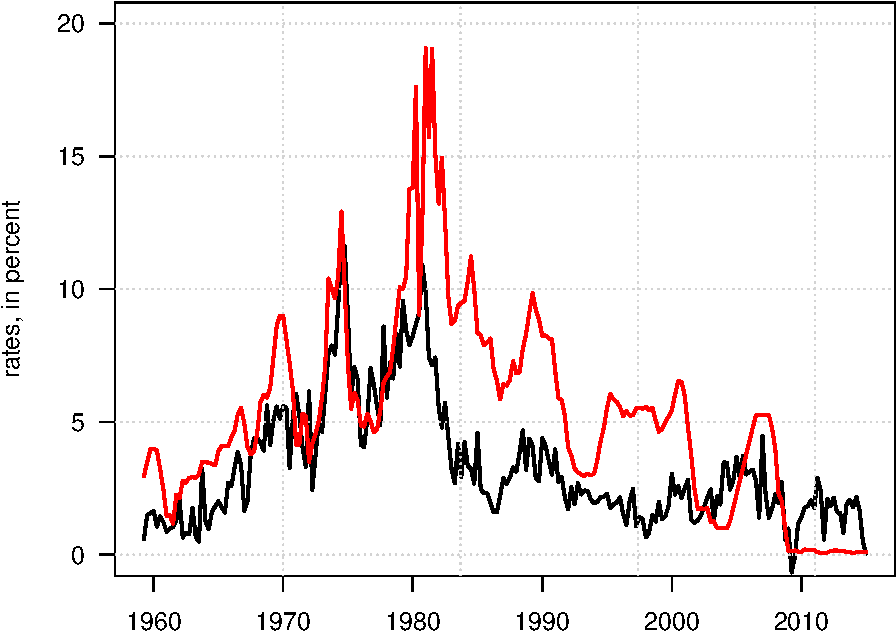
\includegraphics[width=0.95\linewidth]{TimeSeries_files/figure-latex/figInflr-1} \caption{US Inflation and short-term nominal rates.}\label{fig:figInflr}
\end{figure}

Let us now run the tests. Note that the default alternative hypothesis of function \texttt{adf.test} of package \texttt{tseries} is that the process is trend-stationary. Note that when \texttt{kpss.test} returns a p-value of \texttt{0.01}, it means that the true p-value is lower then that.

\begin{Shaded}
\begin{Highlighting}[]
\FunctionTok{library}\NormalTok{(tseries)}
\NormalTok{test.adf.infl }\OtherTok{\textless{}{-}} \FunctionTok{adf.test}\NormalTok{(US3var}\SpecialCharTok{$}\NormalTok{infl,}\AttributeTok{k=}\DecValTok{4}\NormalTok{)}
\NormalTok{test.adf.r    }\OtherTok{\textless{}{-}} \FunctionTok{adf.test}\NormalTok{(US3var}\SpecialCharTok{$}\NormalTok{r,}\AttributeTok{k=}\DecValTok{4}\NormalTok{)}
\NormalTok{test.pp.infl }\OtherTok{\textless{}{-}} \FunctionTok{pp.test}\NormalTok{(US3var}\SpecialCharTok{$}\NormalTok{infl)}
\NormalTok{test.pp.r    }\OtherTok{\textless{}{-}} \FunctionTok{pp.test}\NormalTok{(US3var}\SpecialCharTok{$}\NormalTok{r)}
\NormalTok{test.kpss.infl }\OtherTok{\textless{}{-}} \FunctionTok{kpss.test}\NormalTok{(US3var}\SpecialCharTok{$}\NormalTok{infl)}
\NormalTok{test.kpss.r    }\OtherTok{\textless{}{-}} \FunctionTok{kpss.test}\NormalTok{(US3var}\SpecialCharTok{$}\NormalTok{r)}
\FunctionTok{c}\NormalTok{(test.adf.infl}\SpecialCharTok{$}\NormalTok{p.value,test.pp.infl}\SpecialCharTok{$}\NormalTok{p.value,test.kpss.infl}\SpecialCharTok{$}\NormalTok{p.value)}
\end{Highlighting}
\end{Shaded}

\begin{verbatim}
## [1] 0.29230878 0.04978275 0.01000000
\end{verbatim}

\begin{Shaded}
\begin{Highlighting}[]
\FunctionTok{c}\NormalTok{(test.adf.r}\SpecialCharTok{$}\NormalTok{p.value,test.pp.r}\SpecialCharTok{$}\NormalTok{p.value,test.kpss.r}\SpecialCharTok{$}\NormalTok{p.value)}
\end{Highlighting}
\end{Shaded}

\begin{verbatim}
## [1] 0.3837577 0.3614365 0.0100000
\end{verbatim}

\end{example}

\hypertarget{cointeg}{%
\chapter{Introduction to cointegration}\label{cointeg}}

\hypertarget{intuition}{%
\section{Intuition}\label{intuition}}

Many statistical procedures are well-defined only when the processes of interest are stationary. As a result, especially when one wants to investigate the joint dynamics of different variables, one often begins by making the data stationary (by, e.g., taking first differences or removing deterministic trends). However, doing so may remove information from the data. Heuristically, removing trends amounts to filtering out the long-run variations of the series. However, it may be the case that the different variables interact in the short run \emph{and} in the long run.

For instance, the left plot of Figure \ref{fig:CointegEx} suggests that the trends of \(x_t\) and \(y_t\) are positively correlated. However, the right plot shows that, for low values of \(h\), the correlation between \(x_t - x_{t-h}\) and \(y_t - y_{t-h}\) is negative. This is notably the case for \(h=1\), which means that the first differences of the two variables (i.e., \(\Delta x_t\) and \(\Delta y_t\)) are negatively correlated. Hence, focusing on the first differences would lead the researcher to think that the relationship between \(x_t\) and \(y_t\) is a negative one (while it is only the case when one focuses on the high-frequency comovements between the two variables).

\begin{figure}
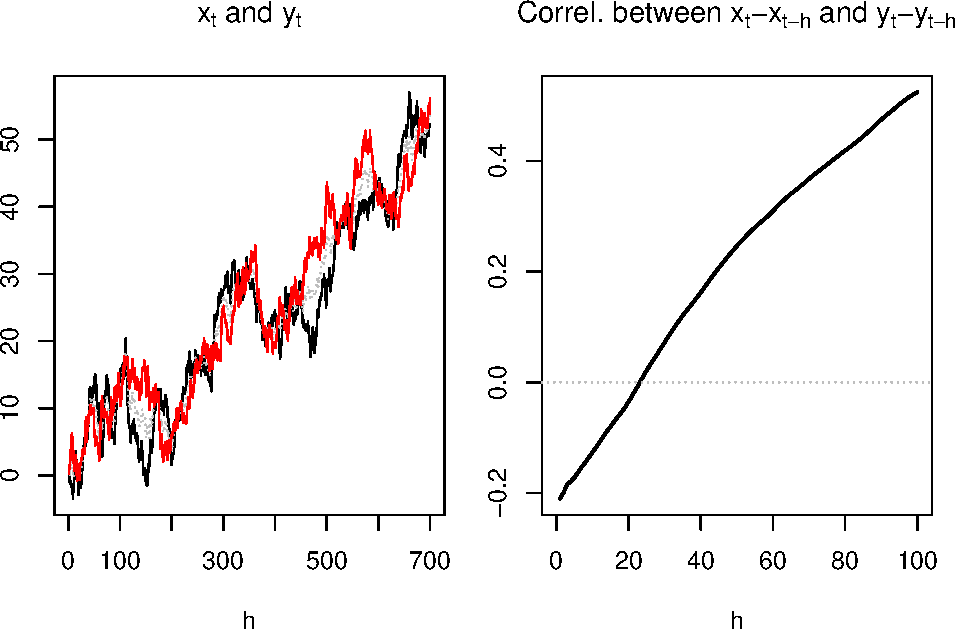
\includegraphics[width=0.95\linewidth]{TimeSeries_files/figure-latex/CointegEx-1} \caption{Situation where the conditional and uncondional correlation between $x_t$ and $y_t$ do not have the same sign.}\label{fig:CointegEx}
\end{figure}

\begin{definition}[Integrated variables]
\protect\hypertarget{def:Id}{}\label{def:Id}A univariate process \(\{y_t\}\) is said to be \(I(d)\) if its \(d^{th}\) difference is stationary (but not its \((d-1)^{th}\) difference).
\end{definition}

For instance:

\begin{itemize}
\tightlist
\item
  If \(y_t\) is not stationary but \(\Delta y_t = y_t - y_{t-1}\) is, then \(y_t\) is \(I(1)\).
\item
  If \(\Delta y_t\) is not stationary but \(\Delta^2 y_t=\Delta(\Delta y_t)\) is, then \(y_t\) is \(I(2)\).
\item
  If \(y_t\) is stationary then \(y_t\) is \(I(0)\).
\end{itemize}

\hypertarget{the-bivariate-case}{%
\section{The bivariate case}\label{the-bivariate-case}}

If we regress an \(I(1)\) variable \(y_t\) on another independent \(I(1)\) variable \(x_t\), the usual (OLS-based) t-tests on regression coefficients often (misleadingly) show statistically significant coefficients (we then speak of spurious regressions, see Section \ref{NonStat}). A solution is to regress \(\Delta y_t\) (that is \(I(0)\)) on \(\Delta x_t\) and then inference will be correct. However, as stated above, the economic interpretation of the regression then changes, as doing so amounts to focusing on the high-frequency movements of the variables.

Let us now consider the case where \(y_t\) and \(x_t\) are still \(I(1)\), but where they satisfy:
\begin{equation}
y_t = \beta x_t + \varepsilon_t,\label{eq:yxI1}
\end{equation}
with \(\varepsilon_t \sim I(0)\). That is, there is a linear combination of the two \(I(1)\) variables that is \(I(0)\).

In that case, the convergence of \(b\), the OLS estimate of \(\beta\), is fast. Indeed, the convergence rate is in \(1/T\) (versus \(1/\sqrt{T}\) in the purely stationary case). This stems from the properties of non-statinary processes that are stated in Prop. \ref{prp:I1process}. We have:
\[
b_T = \frac{\sum_t x_t y_t}{\sum_t x_t^2} = \frac{\sum_t x_t (\beta x_t + \varepsilon_t)}{\sum_t x_t^2}
= \beta + \frac{\sum_t x_t \varepsilon_t}{\sum_t x_t^2}.
\]
In particular, if \(\varepsilon_t\) was a white noise, using properties (ii) and (iv) of Prop. \ref{prp:I1process}, we would get:
\begin{equation}
b_T \approx \beta + \frac{1}{T}\frac{\int_{0}^{1}x_{\infty}(r)dW^{\varepsilon}_r}{\int_{0}^{1}x^2_{\infty}(r)dr}.\label{eq:bTsuperconv}
\end{equation}
where the random variables \(x^2_{\infty}\) and \(W^{\varepsilon}_r\) are defined in Prop. \ref{prp:I1process}.

\begin{proposition}[Properties of an I(1) process]
\protect\hypertarget{prp:I1process}{}\label{prp:I1process}If \(\{y_t\}\) is \(I(1)\) and such that \(y_t - y_{t-1} = H(L)\varepsilon_t\) where \(H(L)\varepsilon_t\) is \(I(0)\), then:

\begin{enumerate}
\def\labelenumi{\roman{enumi}.}
\tightlist
\item
  \(\dfrac{1}{\sqrt{T}}\bar{y}_T \overset{d}{\rightarrow} \int_{0}^{1}y_{\infty}(r)dr\),
\item
  \(\dfrac{1}{T^2}\sum_{t=1}^T y_t^2 \overset{d}{\rightarrow} \int_{0}^{1}y^2_{\infty}(r)dr\),
\item
  \(\dfrac{1}{T}\sum_{t=1}^T y_t(y_t-y_{t-1}) \overset{d}{\rightarrow} \dfrac{1}{2}y^2_{\infty}(1) + \dfrac{1}{2}\mathbb{V}ar(y_t - y_{t-1})\),
\item
  \(\dfrac{1}{T}\sum_{t=1}^T y_t \eta_t \overset{d}{\rightarrow} \sigma_\eta \int_{0}^{1}y_{\infty}(r)dW_r^{\eta}\) where \(\eta_t\) is a white noise of variance \(\sigma_\eta^2\),
\end{enumerate}

where \(y_{\infty}(r)\) is of the form \(\omega W_r\) (\(W_r\) being a Brownian motion (see \href{https://www.dropbox.com/s/w4qc1c32pzkxngv/Simul_Brownian.pdf?dl=0}{extra material}), with \(\omega = \sum_{k=-\infty}^{\infty} \gamma_k\), the \(\gamma_k\)s being the autocovariances of \(H(L)\varepsilon_t\), and where \(\eta_{\infty}(r)\) is of the form \(\sigma_\eta W^{\eta}_r\) (\(W^{\eta}_r\) Brownian motion ``associated'' to \(\eta_t\)).
\end{proposition}

\begin{proof}
(of 1)
We have:
\[
\dfrac{1}{\sqrt{T}}\bar{y}_T = \frac{1}{T}\sum_{t=1}^{T}\frac{y_{t}}{\sqrt{T}} =  \frac{1}{T}\sum_{t=1}^{T}\tilde{y}_T(t/T),
\]
where \(\tilde{y}_T(r)=(1/\sqrt{T})y_{[rT]}\). Now \(\tilde{y}_T(r) = r \sqrt{T} \left(\frac{1}{Tr}\sum_{t=1}^{[Tr]} H(L)\varepsilon_t\right)\). By Eq. \eqref{eq:TCL4ts} in Theorem \ref{thm:CLTcovstat}, we have \(\sqrt{r}\sqrt{Tr} \left(\frac{1}{Tr}\sum_{t=1}^{[Tr]} H(L)\varepsilon_t\right) \rightarrow \omega W_r\). Therefore, for large \(T\), \(\frac{1}{T}\sum_{t=1}^{T}\tilde{y}_T(t/T)\) approximates \(\frac{1}{T}\sum_{t=1}^{T} \omega W_{t/T}\), which is a Riemann sum that converges to \(\int_{0}^{1}y_{\infty}(r)dr\).
\end{proof}

\hypertarget{multivariate-case-and-vecm}{%
\section{Multivariate case and VECM}\label{multivariate-case-and-vecm}}

In the following, we consider an \(n\)-dimensional vector \(y_t\). Moreover, \(\varepsilon_t\) is an \(n\)-dimensional white noise process. The notion of integration (Def. \ref{def:Id}) can also be defined in the multivariate case:

\begin{definition}[Order of integration (multivariate case)]
\protect\hypertarget{def:Idmultivar}{}\label{def:Idmultivar}\(\{y_t\}\) is \(I(d)\) if
\begin{equation}
(1-L)^dy_t = \mu + H(L)\varepsilon_t,\label{eq:I1}
\end{equation}
where \(H(L)\varepsilon_t\) is a stationary process (but \((1-L)^{d-1}y_t\) is not).
\end{definition}

\begin{definition}[Cointegration]
\protect\hypertarget{def:cointegration}{}\label{def:cointegration}If \(y_t\) is integrated of order \(d\), then its components are said to be cointegrated if there exists a linear combination of the components of \(y_t\) that is integrated of an order equal to, or lower than, \(d-1\).
\end{definition}

For instance, Eq. \eqref{eq:yxI1} implies that \([1,-\beta]'\) is a \textbf{cointegrating vector} and that \([x_t,y_t]'\) is cointegrated.

Consider an \(I(1)\) process, \(y_t\), that is such that the Wold representation of \(\Delta y_t\) is Eq. \eqref{eq:I1}. We have:
\[
y_t = \mu + H(L)\varepsilon_t + y_{t-1} = t \mu + H(L)(\varepsilon_t + \varepsilon_{t-1} + \dots + \varepsilon_1) + y_0.
\]

It can be shown that:
\[
y_t = t \mu + H(1)(\varepsilon_t + \varepsilon_{t-1} + \dots + \varepsilon_1) + \xi_t,
\]
where \(\xi_t\) is a stationary process.

Assume that \(y_t\) possesses a cointegrating vector \(\pi\) such that \(\pi' y_t\) is a (univariate) stationary process.

Necessarily, we must have \(\pi' \mu = 0\) and \(\pi' H(1)=0\). Reciprocally, if \(\pi' \mu = 0\) and \(\pi' H(1)=0\), then \(\pi\) is a cointegrating vector of \(y_t\). This proves the following proposition:

\begin{proposition}[Necessary and sufficient conditions of cointegration]
\protect\hypertarget{prp:NScondCoint}{}\label{prp:NScondCoint}If \(y_t\) is \(I(1)\) and admits the Wold representation Eq. \eqref{eq:I1}, with \(d=1\), then \(\pi\) is a cointegrating vector iff
\[
\pi' \mu = 0 \mbox{ (scalar equation) and }\pi' H(1)=0\mbox{ (vectorial equation)}.
\]
\end{proposition}

Consider the following VAR(p) model, where \(y_t\) is \(I(1)\):
\begin{equation}
y_t = c + \Phi_1 y_{t-1} + \dots + \Phi_p y_{t-p} + \varepsilon_t,\label{eq:yVECM1}
\end{equation}
or \(\Phi(L)y_t = c + \varepsilon_t\) where \(\Phi(L) = I - \Phi_1 L - \dots - \Phi_p L^p\).

Suppose that the Wold representation of \(\Delta y_t\) is Eq. \eqref{eq:I1}. Premultiplying Eq. \eqref{eq:I1} by \(\Phi(L)\) gives:
\[
(1-L)\Phi(L)y_t = \Phi(1)\mu + \Phi(L)H(L)\varepsilon_t,
\]
or
\[
(1-L)\varepsilon_t = \Phi(1)\mu + \Phi(L)H(L)\varepsilon_t.
\]
Taking the expectation on both sides gives \(\Phi(1)\mu=0\). Therefore, for the previous equation to hold for any \(\varepsilon_t\), we must have
\[
(1-L) Id = \Phi(L)H(L).
\]
The previous equality implies that \((1-z) Id = \Phi(z)H(z)\) for all \(z\). In particular, for \(z=1\):
\[
0 = \Phi(1)H(1).
\]

Take any row \(\pi'\) of \(\Phi(1)\). Since \(\Phi(1)\mu=0\), we have \(\pi'\mu=0\) (scalar equation). Since \(\Phi(1)H(1)=0\), we have \(\pi' H(1)=0\) (vectorial equation). Prop. \ref{prp:NScondCoint} then implies that the rows of \(\Phi(1)\) are cointegrating vectors of \(y_t\). Therefore, if \(\{a_1,\dots,a_h\}\) constitutes a basis for the space of cointegrating vectors, then \(\pi\) can be expressed as a linear combination of the \(a_i\)'s. That is, we must have:
\[
\pi = [a_1 \quad a_2 \quad \dots \quad a_h]b = \underbrace{A}_{n\times h}\underbrace{b}_{h \times 1},
\]
where \(A = [a_1 \quad a_2 \quad \dots \quad a_h]\).

Since this is true for all rows of \(\Phi(1)\), it comes that this matrix is of the form:
\begin{equation}
\underbrace{\Phi(1)}_{n\times n} = \underbrace{B}_{n\times h}\underbrace{A'}_{h\times n}.\label{eq:BAvecm}
\end{equation}
This shows that the number of independent cointegrating vectors---he order of cointegration of \(y_t\)---is the rank of \(\Phi(1)\). This has important implications for the dynamics of \(\Delta y_t\).

Consider a process \(y_t\) whose VAR representation is as in Eq. \eqref{eq:yVECM1}. This VAR representation can be rewritten:
\begin{equation}
y_t = (c + \rho y_{t-1}) + \zeta_1 \Delta y_{t-1} + \dots + \zeta_{p-1} \Delta y_{t-p+1} + \varepsilon_t,\label{eq:yVECM2}
\end{equation}
where \(\zeta_k = - \Phi_{k+1} - \dots - \Phi_{p}\) and \(\rho = \Phi_1 + \dots + \Phi_p\).

\begin{example}[VAR(2)]
\protect\hypertarget{exm:vecmVAR2}{}\label{exm:vecmVAR2}For a VAR(2) with \(y_t = c + \Phi_1 y_{t-1}+ \Phi_2 y_{t-2} + \varepsilon_t\), we have:
\[
y_t = c + \{\Phi_1 + \Phi_2\} y_{t-1} + \{-\Phi_2\} \Delta y_{t-1} + \varepsilon_t,
\]
\end{example}

Subtracting \(y_{t-1}\) from both sides of Eq. \eqref{eq:yVECM2} and remarking that \(-\Phi(1) = \rho - Id\) (recall that \(\Phi(L) = I - \Phi_1 L - \dots - \Phi_p L^p\)), we get:
\[
\Delta y_t = \{c - \underbrace{\Phi(1) y_{t-1}}_{=BA'y_{t-1}}\} + \zeta_1 \Delta y_{t-1} + \dots + \zeta_{p-1} \Delta y_{t-p+1} + \varepsilon_t.
\]

Using Eq. \eqref{eq:BAvecm}, and denoting by \(z_t\) the \(h\)-dimensional vector \(A'y_{t}\), we obtain the \textbf{error correction representation} of the cointegrated variable \(y_t\):
\begin{equation}
\boxed{\Delta y_t = c - B z_{t-1} + \zeta_1 \Delta y_{t-1} + \dots + \zeta_{p-1} \Delta y_{t-p+1} + \varepsilon_t.}\label{eq:VECM3}
\end{equation}
This type of model is called \textbf{Vector Error Correction Model} (VECM). This is because the components of \(z_t\) can be considered as errors that, multiplied by the components of \(B\) generate correction forces that imply that, in the long run, the congregation relationships are satisfied. Example \ref{exm:ExampleVECM1} illustrates this.

\begin{example}[VECM example]
\protect\hypertarget{exm:ExampleVECM1}{}\label{exm:ExampleVECM1}

Consider the VAR(1) process \(y_t\) that follows:
\[
y_t = \Phi_1 y_{t-1} + \varepsilon_t = \left[\begin{array}{cc}
0.5 & 0.5 \\
0.2 & 0.8 \\
\end{array}
\right] y_{t-1} + \varepsilon_t, \quad \varepsilon_t \sim i.i.d. \mathcal{N}(0,\Sigma)
\]

1 is an eigenvalue of \(\Phi_1\) and \(y_t\) is \(I(1)\). We have:
\[
\Phi(1) = Id - \left[\begin{array}{cc}
0.5 & 0.5 \\
0.2 & 0.8 \\
\end{array}
\right] = \left[\begin{array}{cc}
0.5 & -0.5 \\
-0.2 & 0.2 \\
\end{array}
\right],
\]
which is of rank 1. Therefore \(y_t\) is cointegrated of order 1.

For that process, Eq. \eqref{eq:VECM3} writes:
\[
\Delta y_{t} =
- \left[\begin{array}{cc}
0.5 & -0.5 \\
-0.2 & 0.2
\end{array}
\right] y_{t-1} + \varepsilon_t =
\left[\begin{array}{c}
-0.5\\
0.2
\end{array}
\right] z_{t-1} + \varepsilon_t,
\]
where \(z_{t} = y_{1,t}-y_{2,t}\).

The process \(z_t\) is stationary (we have \(z_t = 0.3 z_{t-1} + \varepsilon_{1,t} - \varepsilon_{2,t}\)).

We say that there is a \emph{long-run relationship} between \(y_{1,t}\) and \(y_{2,t}\):

When \(y_{1,t}\) is substantially above \(y_{2,t}\), \(z_t\) is large, the influence of \(-0.5 z_t\) on \(\Delta y_{1,t+1}\) is negative, which tends to ``correct'' \(y_{1,t}\) and brings it closer to \(y_{2,t}\).

\begin{figure}
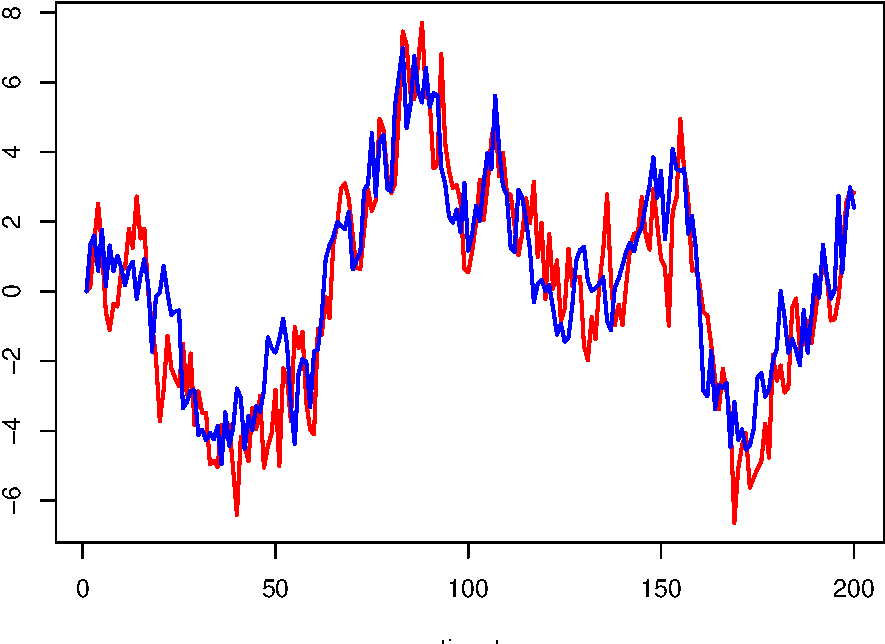
\includegraphics[width=0.95\linewidth]{TimeSeries_files/figure-latex/VECMexmpl-1} \caption{Simulation of $y_{1,t}$ (in blue) and $y_{2,t}$ (in red).}\label{fig:VECMexmpl}
\end{figure}

\end{example}

\hypertarget{cointegration-in-practice}{%
\subsection{Cointegration in practice}\label{cointegration-in-practice}}

Assume that we have a vector of variables \(y_t\) and that we want to investigate the joint dynamics of its components. If the \(y_{i,t}\)s are \(I(1)\), we may need to use a VECM. Therefore, in the first place, one has to test for the stationarity of \(y_t\)'s components (see Section \ref{NonStat}).

If the components of \(y_t\) are \(I(1)\), one has to determine the existence of cointegrating vectors. There are two general possibilities to do this:

\begin{enumerate}
\def\labelenumi{\arabic{enumi}.}
\tightlist
\item
  The theory provides us with relevant cointegration relationships, for instance:

  \begin{itemize}
  \tightlist
  \item
    The Purchasing Power Parity (PPP) suggests the existence of a long-run relationship between domestic prices, foreign prices, and the exchange rate.
  \item
    If real rates are stationary, the Fisher equation (\(r=i-\pi\)) implies a cointegration relatinsip between the nominal interest rate (\(i\)) and inflation \(\pi\).
  \end{itemize}
\item
  We have no a priori regarding the cointegration relationship. We have to estimate (and test) the potential cointegration relationship.
\end{enumerate}

In the first case, we proceed in two steps:
a. If \(\pi^*\) is suspected to be a cointegrating vector, we can then use unit-root or stationarity tests on \(z_t={\pi^*}' y_t\) (see Section @ref\{NonStat\}).
b. Estimate Eq. \eqref{eq:VECM3} by OLS.

In the following, we focus on the second case, when there is at most one cointegration relationship. (In the general case, one can for instance implement the \citet{Johansen_1991} approach.)

\citet{Engle_Granger_1987} propose a two-step estimation procedure to estimate error-correction models. This method proceeds under the assumption that there is a single cointegration equation, i.e.~\(A' = [\alpha_1,\dots,\alpha_n]\). (Recall that \(\Phi(1) = BA'\), see Eq. \eqref{eq:BAvecm}.) Without loss of generality, one can set \(\alpha_1=1\). In that case, the cointegration relationship, if it exists, is of the form:
\[
y_{1,t} = - \alpha_2 y_{2,t} - \dots - \alpha_n y_{n,t} + z_t,
\]
where \(z_t \sim I(0)\).

The first step consists in estimating the previous equation by OLS (regression of \(y_{1,t}\) on \(y_{2,t},\dots,y_{2,t}\)). The second step consists in estimating Eq. \eqref{eq:VECM3} also by OLS, after having replaced \(z_{t-1}\) by the (lagged) residuals of the first step OLS regression (\(\hat{z}_{t-1}\)). Because of high speed convergence of the first-step regression (the convergence is in \(1/T\), see Eq. \eqref{eq:bTsuperconv}), the asymptotic properties of the second-step estimates are the standard ones. That is, one can use the standard t-statistic to assess the statistical significativity of the parameters.

It remains to explain how to test for the existence of a cointegration relationship. This amounts to testing whether \(z_t\) is stationary. Note however that we do not observe the ``true'' \(z_t\), but only OLS-based estimates \(\hat{z}_t\). Therefore, the critical values of the usual unit-root tests are not the same. The appropriate critical values are given by \citet{Phillips_Ouliaris_1990}.

\begin{example}[VECM for US inflation and nominal interest rate]
\protect\hypertarget{exm:VECMUS}{}\label{exm:VECMUS}The data are as in Example \ref{exm:NonStatExample}. In the first step, we compute \(z_t\) and use \citet{Phillips_Ouliaris_1990}'s test to see whether the two variables are cointegrated:

\begin{Shaded}
\begin{Highlighting}[]
\FunctionTok{library}\NormalTok{(AEC);}\FunctionTok{library}\NormalTok{(tseries)}
\NormalTok{T }\OtherTok{\textless{}{-}} \FunctionTok{dim}\NormalTok{(US3var)[}\DecValTok{1}\NormalTok{]}
\NormalTok{infl }\OtherTok{\textless{}{-}}\NormalTok{ US3var}\SpecialCharTok{$}\NormalTok{infl}
\NormalTok{i    }\OtherTok{\textless{}{-}}\NormalTok{ US3var}\SpecialCharTok{$}\NormalTok{r}
\NormalTok{eq }\OtherTok{\textless{}{-}} \FunctionTok{lm}\NormalTok{(i}\SpecialCharTok{\textasciitilde{}}\NormalTok{infl)}
\NormalTok{z }\OtherTok{\textless{}{-}}\NormalTok{ eq}\SpecialCharTok{$}\NormalTok{residuals}
\FunctionTok{po.test}\NormalTok{(}\FunctionTok{cbind}\NormalTok{(i,infl))}
\end{Highlighting}
\end{Shaded}

\begin{verbatim}
## 
##  Phillips-Ouliaris Cointegration Test
## 
## data:  cbind(i, infl)
## Phillips-Ouliaris demeaned = -29.484, Truncation lag parameter = 2,
## p-value = 0.01
\end{verbatim}

We reject the null hypothesis of unit root in the residuals. That is, the results are in favor of cointegration. Let us then esitmate the VECM model; this amounts to running two OLS regressions:

\begin{Shaded}
\begin{Highlighting}[]
\NormalTok{infl\_1 }\OtherTok{\textless{}{-}} \FunctionTok{c}\NormalTok{(}\ConstantTok{NaN}\NormalTok{,infl[}\DecValTok{1}\SpecialCharTok{:}\NormalTok{(T}\DecValTok{{-}1}\NormalTok{)])}
\NormalTok{infl\_2 }\OtherTok{\textless{}{-}} \FunctionTok{c}\NormalTok{(}\ConstantTok{NaN}\NormalTok{,}\ConstantTok{NaN}\NormalTok{,infl[}\DecValTok{1}\SpecialCharTok{:}\NormalTok{(T}\DecValTok{{-}2}\NormalTok{)])}
\NormalTok{infl\_3 }\OtherTok{\textless{}{-}} \FunctionTok{c}\NormalTok{(}\ConstantTok{NaN}\NormalTok{,}\ConstantTok{NaN}\NormalTok{,}\ConstantTok{NaN}\NormalTok{,infl[}\DecValTok{1}\SpecialCharTok{:}\NormalTok{(T}\DecValTok{{-}3}\NormalTok{)])}
\NormalTok{i\_1 }\OtherTok{\textless{}{-}} \FunctionTok{c}\NormalTok{(}\ConstantTok{NaN}\NormalTok{,i[}\DecValTok{1}\SpecialCharTok{:}\NormalTok{(T}\DecValTok{{-}1}\NormalTok{)])}
\NormalTok{i\_2 }\OtherTok{\textless{}{-}} \FunctionTok{c}\NormalTok{(}\ConstantTok{NaN}\NormalTok{,}\ConstantTok{NaN}\NormalTok{,i[}\DecValTok{1}\SpecialCharTok{:}\NormalTok{(T}\DecValTok{{-}2}\NormalTok{)])}
\NormalTok{i\_3 }\OtherTok{\textless{}{-}} \FunctionTok{c}\NormalTok{(}\ConstantTok{NaN}\NormalTok{,}\ConstantTok{NaN}\NormalTok{,}\ConstantTok{NaN}\NormalTok{,i[}\DecValTok{1}\SpecialCharTok{:}\NormalTok{(T}\DecValTok{{-}3}\NormalTok{)])}
\NormalTok{z\_1 }\OtherTok{\textless{}{-}} \FunctionTok{c}\NormalTok{(}\ConstantTok{NaN}\NormalTok{,z[}\DecValTok{1}\SpecialCharTok{:}\NormalTok{(T}\DecValTok{{-}1}\NormalTok{)])}
\NormalTok{dinfl   }\OtherTok{\textless{}{-}}\NormalTok{ infl   }\SpecialCharTok{{-}}\NormalTok{ infl\_1}
\NormalTok{dinfl\_1 }\OtherTok{\textless{}{-}}\NormalTok{ infl\_1 }\SpecialCharTok{{-}}\NormalTok{ infl\_2}
\NormalTok{dinfl\_2 }\OtherTok{\textless{}{-}}\NormalTok{ infl\_2 }\SpecialCharTok{{-}}\NormalTok{ infl\_3}
\NormalTok{di   }\OtherTok{\textless{}{-}}\NormalTok{ i   }\SpecialCharTok{{-}}\NormalTok{ i\_1}
\NormalTok{di\_1 }\OtherTok{\textless{}{-}}\NormalTok{ i\_1 }\SpecialCharTok{{-}}\NormalTok{ i\_2}
\NormalTok{di\_2 }\OtherTok{\textless{}{-}}\NormalTok{ i\_2 }\SpecialCharTok{{-}}\NormalTok{ i\_3}
\NormalTok{eq1 }\OtherTok{\textless{}{-}} \FunctionTok{lm}\NormalTok{(di    }\SpecialCharTok{\textasciitilde{}}\NormalTok{ z\_1 }\SpecialCharTok{+}\NormalTok{ dinfl\_1 }\SpecialCharTok{+}\NormalTok{ di\_1 }\SpecialCharTok{+}\NormalTok{ dinfl\_2 }\SpecialCharTok{+}\NormalTok{ di\_2)}
\NormalTok{eq2 }\OtherTok{\textless{}{-}} \FunctionTok{lm}\NormalTok{(dinfl }\SpecialCharTok{\textasciitilde{}}\NormalTok{ z\_1 }\SpecialCharTok{+}\NormalTok{ dinfl\_1 }\SpecialCharTok{+}\NormalTok{ di\_1 }\SpecialCharTok{+}\NormalTok{ dinfl\_2 }\SpecialCharTok{+}\NormalTok{ di\_2)}
\end{Highlighting}
\end{Shaded}

Table \ref{tab:EngleGrangerUS3} reports the estimated coefficients in \texttt{eq1} and \texttt{eq2}, together with their p-values:

\begin{table}

\caption{\label{tab:EngleGrangerUS3}Results of the second-stage OLS regressions (Engle-Granger approach). The first variable is the short-term nominal interest rate; the second variable is inflation.}
\centering
\begin{tabular}[t]{l|r|r|r|r}
\hline
  & Coef Y1 & p-values Y1 & Coef Y2 & p-values Y2\\
\hline
(Intercept) & -0.0189 & 0.8093 & -0.0047 & 0.9457\\
\hline
z\_1 & -0.1040 & 0.0014 & -0.0034 & 0.9046\\
\hline
dinfl\_1 & 0.0224 & 0.7852 & -0.3845 & 0.0000\\
\hline
di\_1 & -0.0841 & 0.2225 & 0.1196 & 0.0473\\
\hline
dinfl\_2 & 0.0322 & 0.6864 & -0.2238 & 0.0014\\
\hline
di\_2 & -0.0393 & 0.5625 & 0.0828 & 0.1626\\
\hline
\end{tabular}
\end{table}

Imporantly, one of the parameters associated with \(z_{t-1}\) (parameters that are called speeds of adjustement) is significant and with the expected signs: if the short term nominal interest rate \(i_t\) is high then \(z_t\) becomes positive (since, up to an intercept, \(z_t = i_t - \beta \pi_t\), where \(\beta\) comes from the first-step regression), but since \(B_{1,1}\) is negative (it is equal to -0.104), a positive \(z_t\) will generate a negative correction (i.e., \(B_{1,1}z_t\)) for \(i_{t+1}\) on date \(t+1\), thereby ``correcting'' the high level of \(i_t\).
\end{example}

\hypertarget{ARCHGARCH}{%
\chapter{ARCH and GARCH models}\label{ARCHGARCH}}

\hypertarget{conditional-heteroskedasticity}{%
\section{Conditional heteroskedasticity}\label{conditional-heteroskedasticity}}

Many financial and macroeconomic variables are hit by shocks whose variance is not constant through time, i.e.~by \emph{heteroskedatic} shocks. Often, the conditional variance of shocks features a persistent behavior (volatility clustering). The observation that large shocks (in absolute value) tend to be followed by other important shocks has notably been established by \citet{Mandelbrot_1963}. Such a situation is illustrated by Figure \ref{fig:GARCHsmireturns}.

Autoregressive Conditional Heteroskedasticity (ARCH) and its generalized version (GARCH) constitute useful tools to model such time series.

\begin{figure}
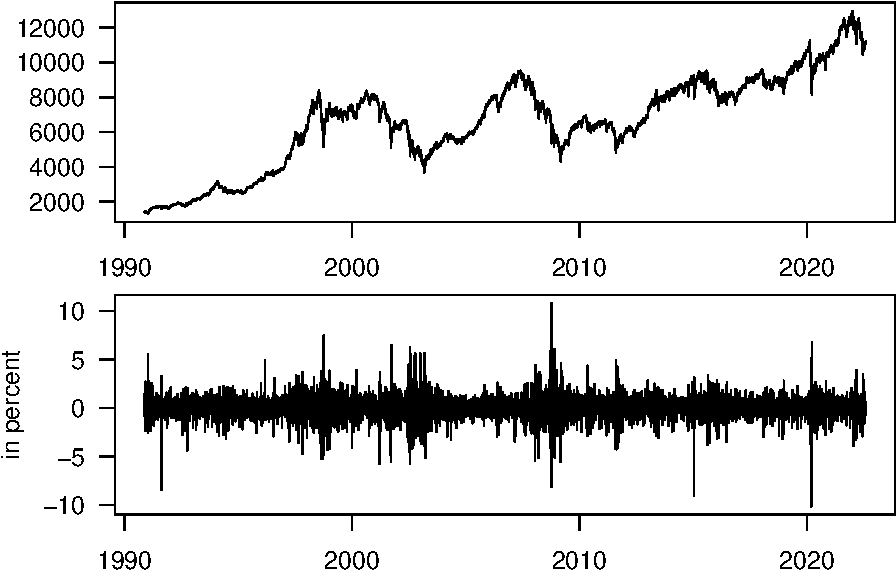
\includegraphics[width=1\linewidth]{TimeSeries_files/figure-latex/GARCHsmireturns-1} \caption{Upper plot: SMI index (daily Close prices); lower plot: daily log returns.}\label{fig:GARCHsmireturns}
\end{figure}

In order to test whether a times series of shocks \(\{u_1,\dots,u_T\}\) features persistent conditional heteroskedasticity, a simple test has been designed by \citet{Engle_1982}. This test consists in regressing \(u_t^2\) on it last \(m\) lags (i.e., on \(u_{t-1}^2,\dots,u_{t-m}^2\)) by OLS.Under the null hypothesis that \(u_t\) is i.i.d., we have:
\[
T \times R^2 \overset{d}{\rightarrow} \chi^2(m),
\]
where \(R^2\) is the centered \(R^2\) of the OLS regression.

Let us employ this test on the return series plotted in the lower panel of Figure \ref{fig:GARCHsmireturns}:

\begin{Shaded}
\begin{Highlighting}[]
\FunctionTok{library}\NormalTok{(AEC);}\FunctionTok{data}\NormalTok{(smi)}
\NormalTok{smi }\OtherTok{\textless{}{-}}\NormalTok{ smi[}\FunctionTok{complete.cases}\NormalTok{(smi),] }\CommentTok{\# remove NaNs}
\NormalTok{T }\OtherTok{\textless{}{-}} \FunctionTok{dim}\NormalTok{(smi)[}\DecValTok{1}\NormalTok{]}
\NormalTok{smi}\SpecialCharTok{$}\NormalTok{r }\OtherTok{\textless{}{-}} \DecValTok{100}\SpecialCharTok{*}\FunctionTok{c}\NormalTok{(}\ConstantTok{NaN}\NormalTok{,}\FunctionTok{log}\NormalTok{(smi}\SpecialCharTok{$}\NormalTok{Close[}\DecValTok{2}\SpecialCharTok{:}\NormalTok{T]}\SpecialCharTok{/}\NormalTok{smi}\SpecialCharTok{$}\NormalTok{Close[}\DecValTok{1}\SpecialCharTok{:}\NormalTok{(T}\DecValTok{{-}1}\NormalTok{)]))}
\NormalTok{u }\OtherTok{\textless{}{-}}\NormalTok{ smi}\SpecialCharTok{$}\NormalTok{r}\SpecialCharTok{\^{}}\DecValTok{2}
\NormalTok{u\_1 }\OtherTok{\textless{}{-}} \FunctionTok{c}\NormalTok{(}\ConstantTok{NaN}\NormalTok{,smi}\SpecialCharTok{$}\NormalTok{r[}\DecValTok{1}\SpecialCharTok{:}\NormalTok{(T}\DecValTok{{-}1}\NormalTok{)]}\SpecialCharTok{\^{}}\DecValTok{2}\NormalTok{)}
\NormalTok{u\_2 }\OtherTok{\textless{}{-}} \FunctionTok{c}\NormalTok{(}\ConstantTok{NaN}\NormalTok{,}\ConstantTok{NaN}\NormalTok{,smi}\SpecialCharTok{$}\NormalTok{r[}\DecValTok{1}\SpecialCharTok{:}\NormalTok{(T}\DecValTok{{-}2}\NormalTok{)]}\SpecialCharTok{\^{}}\DecValTok{2}\NormalTok{)}
\NormalTok{eq }\OtherTok{\textless{}{-}} \FunctionTok{lm}\NormalTok{(u}\SpecialCharTok{\^{}}\DecValTok{2} \SpecialCharTok{\textasciitilde{}}\NormalTok{ u\_1}\SpecialCharTok{\^{}}\DecValTok{2} \SpecialCharTok{+}\NormalTok{ u\_2}\SpecialCharTok{\^{}}\DecValTok{2}\NormalTok{)}
\NormalTok{test.stat }\OtherTok{\textless{}{-}} \FunctionTok{length}\NormalTok{(u)}\SpecialCharTok{*}\FunctionTok{summary}\NormalTok{(eq)}\SpecialCharTok{$}\NormalTok{r.squared}
\NormalTok{pvalue }\OtherTok{\textless{}{-}} \DecValTok{1} \SpecialCharTok{{-}} \FunctionTok{pchisq}\NormalTok{(}\AttributeTok{q =}\NormalTok{ test.stat,}\AttributeTok{df=}\DecValTok{2}\NormalTok{)}
\end{Highlighting}
\end{Shaded}

The p-value is extremely close to zero. Hence we strongly reject the null of an i.i.d. SMI return.

\hypertarget{ARCH}{%
\section{The ARCH model}\label{ARCH}}

\hypertarget{the-two-arch-specifications}{%
\subsection{The two ARCH specifications}\label{the-two-arch-specifications}}

Consider the auto-regressive process following:
\begin{equation}
y_t = c + \phi_1 y_{t-1} + \dots + \phi_p y_{t-p} + u_t,\label{eq:linearreg}
\end{equation}
where \(u_t\) is a white noise (Def. \ref{def:whitenoise}), i.e.~\(\mathbb{E}(u_t)=0\), \(\mathbb{E}(u_t^2)=\sigma^2\) and \(\mathbb{E}(u_t u_s)=0\) if \(s \ne t\). Importantly, note that while the \emph{unconditional variance} of \(u_t\) is \(\sigma^2\), its \emph{conditional variance} can be time-varying. This is the case in the context of (G)ARCH models.

In the ARCH(m) model, \(u_t\) follows:
\begin{equation}
u_t^2 = \zeta + \alpha_1 u_{t-1}^2 + \dots + \alpha_m u_{t-m}^2 + w_t,\label{eq:ut2}
\end{equation}
where \(w_t\) is a non-autocorrelated white noise process that is exogenous to \(u_t\), in the sense that:
\[
\mathbb{E}(w_t|u_{t-1},u_{t-2},\dots)=0.
\]
In this case:
\begin{equation}
\mathbb{E}(u_t^2|u_{t-1},u_{t-2},\dots) = \zeta + \alpha_1 u_{t-1}^2 + \dots + \alpha_m u_{t-m}^2.\label{eq:condvar}
\end{equation}

For Eq. \eqref{eq:ut2} to make sense, it has to be the case that
\[
\zeta + \alpha_1 u_{t-1}^2 + \dots + \alpha_m u_{t-m}^2 + w_t \le 0
\]
for all realisations of \(\{u_t\}\). This is the case if \(w_t > -\zeta\), with \(\zeta>0\), and if \(\alpha_i \ge 0\) for \(i \in \{1,\dots,m\}\). Assuming this is the case, \(u_t^2\) is covariance-stationary if the roots of:
\[
g(z) = 1 - \alpha_1 z - \dots - \alpha_m z^m = 0
\]
lie outside the unit circle (Prop. \ref{prp:stability}). A necessary condition for not having a root between 0 and 1 is that \(\sum_i \alpha_i<1\).\footnote{If we have \(1-\sum_i \alpha_i \le 0\), then \(g(1) \le 0\). We would then have \(g(0)=1>0\) and \(g(1)\le 0\). Since \(g\) is continuous, this would imply that \(\exists z \in [0,1]\) s.t. \(g(z)=0\).} This is also a sufficient condition.\footnote{Indeed, for \(z \in [-1,1]\), we have \(1 - \alpha_1 z - \dots - \alpha_m z^m \ge 1 - \sum_i |\alpha_iz^i| \ge 1 - \sum_i \alpha_i > 0\).}

If \(w_t > -\zeta\), with \(\zeta>0\), \(\alpha_i\ge0\) for \(i \in \{1,\dots,m\}\) and \(\sum_i \alpha_i<1\), then the unconditional variance of \(u_t\) is:
\[
\sigma^2 = \mathbb{E}(u_t^2) = \frac{\zeta}{1 - \sum_{i=1}^m \alpha_i}.
\]

An alternative representation of an ARCH(m) process is as follows:
\begin{equation}
u_t = \sqrt{h_t}v_t,\label{eq:uhv}
\end{equation}
where \(v_t\) is an i.i.d. sequence with zero mean and unit variance, i.e.:
\[
\mathbb{E}(v_t) = 0, \quad \mathbb{E}(v_t^2) = 1.
\]
If \(h_t\) follows:
\begin{equation}
h_t = \zeta + \alpha_1 u_{t-1}^2 + \dots + \alpha_m u_{t-m}^2,\label{eq:hARCH}
\end{equation}
then Eq. \eqref{eq:condvar} is also true. Since \(u_t^2 = h_t v_t^2\), Eq. \eqref{eq:ut2} holds with \(w_t = h_t (v_t^2-1)\). This alternative representation is convenient because \(v_t\) is not necessarily bounded.

\hypertarget{maximum-likelihood-estimation-of-an-arch-process}{%
\subsection{Maximum Likelihood Estimation of an ARCH process}\label{maximum-likelihood-estimation-of-an-arch-process}}

Assume the complete model is:
\[
y_t = \mathbf{x}_t'\boldsymbol\beta + u_t,
\]
where \(\mathbf{x}_t\) is a \(k \times 1\) vector of explanatory variables and \(u_t\) is as specified in Eq. \eqref{eq:uhv}.

To write the likelihood function, it is convenient to condition on the first \(m\) observations. Let us denote by \(\mathcal{I}_t\) the following information set:
\[
\mathcal{I}_t = (y_t,y_{t-1},\dots,y_0,y_{-1},\dots,y_{-m+1}, \mathbf{x}_t,\mathbf{x}_{t-1},\dots,\mathbf{x}_0,\mathbf{x}_{-1},\dots,\mathbf{x}_{-m+1}).
\]

If \(v_t \sim \mathcal{N}(0,1)\), we have, for \(t\ge1\):
\begin{equation}
f(y_t|\mathbf{x_t},\mathcal{I}_{t-1}) = \frac{1}{\sqrt{2 \pi h_t}}\exp\left(\frac{-(y_t-\mathbf{x}_t'\boldsymbol\beta)^2}{2h_t}\right),\label{eq:densityN}
\end{equation}
where \(h_t\) is given by:
\[
h_t = \zeta + \alpha_1 (y_{t-1} - \mathbf{x}_{t-1}'\boldsymbol\beta)^2 + \dots + \alpha_m (y_{t-m} - \mathbf{x}_{t-m}'\boldsymbol\beta)^2.
\]

The log likelihood function is given by:
\[
\log \mathcal{L}(\theta) = \sum_{t=1}^T \log(f(y_t|\mathbf{x_t},\mathcal{I}_{t-1})),
\]
where \(\theta\), the vector of unknown parameters, is \([\boldsymbol\beta',\zeta,\boldsymbol\alpha']'\), where \(\boldsymbol\alpha=[\alpha_1,\dots,\alpha_m]'\). The maximisation of the log likelihood is performed numerically.

Note that one can also use non-Gaussian distributions for \(v_t\). (For that, one has to replace the normal distribution in Eq. \eqref{eq:densityN}.)

Let us fit an ARCH(2) model on the SMI return data (lower plot of Figure \ref{fig:GARCHsmireturns}). For this, we make use of function \texttt{compute.garch} of package \texttt{AEC}. This function takes four arguments:

\begin{itemize}
\tightlist
\item
  vector \texttt{theta} contains the model parameterization: first, \(\zeta\), then the \(\alpha_i\)'s, then for GARCH models (see Subsection \ref{GARCH} below), the \(\delta_i\)'s.
\item
  vector \texttt{x} contains the observations of the process.
\item
  \texttt{m} is the number of lags in the ARCH specification.
\item
  \texttt{r} is the number of lags in the GARCH specification (see Subsection \ref{GARCH} below).
\end{itemize}

Function \texttt{compute.garch} returns a list, one entry of each is the log-likelihood associated with a parameterization \([\zeta,\boldsymbol\alpha']'\), the second being the resulting sequence of \(h_t\)'s (see Eq. \eqref{eq:hARCH}). Let us create a function that returns only the log-likelihood:

\begin{Shaded}
\begin{Highlighting}[]
\NormalTok{loglik }\OtherTok{\textless{}{-}} \ControlFlowTok{function}\NormalTok{(theta,x,m,r)\{}
  \CommentTok{\# first parameter of theta: zeta}
  \CommentTok{\# next: alpha\textquotesingle{}s (ARCH)}
  \CommentTok{\# next: delta\textquotesingle{}s (GARCH)}
\NormalTok{  Garch }\OtherTok{\textless{}{-}} \FunctionTok{compute.garch}\NormalTok{(theta,x,m,r)}
  \FunctionTok{return}\NormalTok{(Garch}\SpecialCharTok{$}\NormalTok{logf)}
\NormalTok{\}}
\end{Highlighting}
\end{Shaded}

Now, let us maximize the log-likelihood:

\begin{Shaded}
\begin{Highlighting}[]
\NormalTok{m }\OtherTok{\textless{}{-}} \DecValTok{2}
\NormalTok{r }\OtherTok{\textless{}{-}} \DecValTok{0} \CommentTok{\# for ARCH models, r=0}
\NormalTok{smi }\OtherTok{\textless{}{-}}\NormalTok{ smi[}\DecValTok{4000}\SpecialCharTok{:}\FunctionTok{dim}\NormalTok{(smi)[}\DecValTok{1}\NormalTok{],] }\CommentTok{\# reduce sample}
\NormalTok{par0 }\OtherTok{\textless{}{-}} \FunctionTok{c}\NormalTok{(}\FloatTok{0.62}\NormalTok{,}\FloatTok{0.2}\NormalTok{,}\FloatTok{0.2}\NormalTok{)}
\NormalTok{res.opt }\OtherTok{\textless{}{-}} \FunctionTok{optim}\NormalTok{(}\AttributeTok{par=}\NormalTok{par0,}\AttributeTok{x=}\NormalTok{smi}\SpecialCharTok{$}\NormalTok{r,}\AttributeTok{m=}\NormalTok{m,}\AttributeTok{r=}\NormalTok{r,loglik,}
                 \AttributeTok{method=}\StringTok{"BFGS"}\NormalTok{,}\AttributeTok{hessian=}\ConstantTok{TRUE}\NormalTok{,}
                 \AttributeTok{control =} \FunctionTok{list}\NormalTok{(}\AttributeTok{trace=}\ConstantTok{TRUE}\NormalTok{,}\AttributeTok{maxit =} \DecValTok{10}\NormalTok{))}
\NormalTok{estim.param }\OtherTok{\textless{}{-}}\NormalTok{ res.opt}\SpecialCharTok{$}\NormalTok{par}
\NormalTok{std.dev }\OtherTok{\textless{}{-}} \FunctionTok{sqrt}\NormalTok{(}\FunctionTok{diag}\NormalTok{(}\FunctionTok{solve}\NormalTok{(res.opt}\SpecialCharTok{$}\NormalTok{hessian)))}
\NormalTok{t.stat }\OtherTok{\textless{}{-}}\NormalTok{ estim.param}\SpecialCharTok{/}\NormalTok{std.dev}
\end{Highlighting}
\end{Shaded}

Table \ref{tab:estimGARCH2} reports the estimated parameters and their standard deviation. Figure \ref{fig:estimGARCH3} displays the resulting 95\% confidence intervals (i.e., \(\pm 2 \sqrt{h_t}\)).

\begin{table}

\caption{\label{tab:estimGARCH2}ARCH(2), ML estimation results.
             Data: SMI daily returns.}
\centering
\begin{tabular}[t]{l|r|r|r}
\hline
  & Estim. param. & Std dev. & t-stat\\
\hline
zeta & 0.6042 & 0.0230 & 26.3054\\
\hline
alpha1 & 0.2939 & 0.0289 & 10.1704\\
\hline
alpha2 & 0.2321 & 0.0250 & 9.2838\\
\hline
\end{tabular}
\end{table}

\begin{figure}
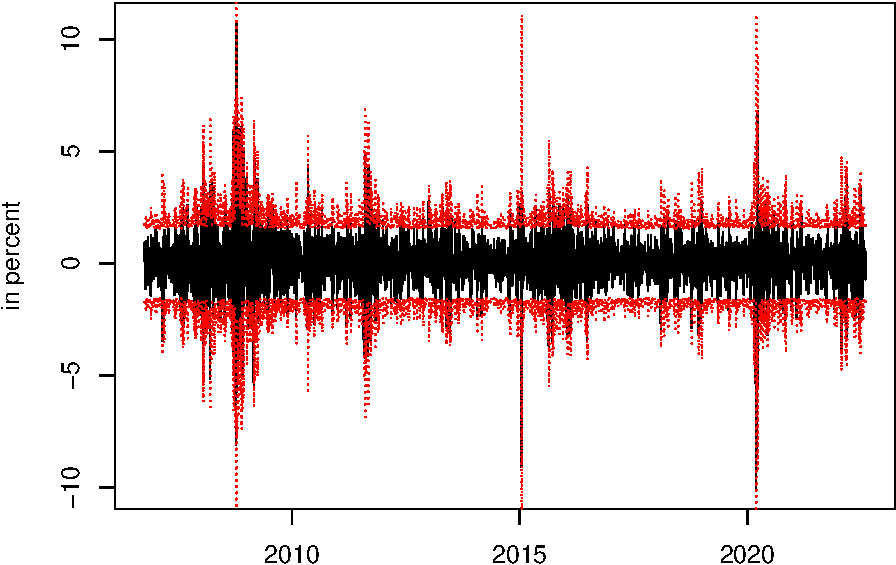
\includegraphics{TimeSeries_files/figure-latex/estimGARCH3-1} \caption{SMI daily returns (in black) and, in red, 95\% confidence interval based on the ARCH(2) estimated model ($\pm 2 \sqrt{h_t}$).}\label{fig:estimGARCH3}
\end{figure}

\hypertarget{GARCH}{%
\section{The GARCH model}\label{GARCH}}

One can generalize the model and replace Eq. \eqref{eq:hARCH} with:
\begin{eqnarray}
h_t &=& (1-\delta_1 - \delta_2 - \dots - \delta_r) \zeta + \nonumber \\
&&\delta_1 h_{t-1} + \delta_2 h_{t-2} + \dots + \delta_r h_{t-r} + \nonumber \\
&&\alpha_1 u_{t-1}^2 + \dots + \alpha_m u_{t-m}^2. \label{eq:hGARCH}
\end{eqnarray}
This generalised autoregressive conditional heteroskedasticity model is denoted by GARCH(r,m). Non-negativity is satisfied as soon as \(\kappa>0\), \(\alpha_j \ge 0\), \(\delta_j \ge 0\) for \(j \le p\).

Denoting \(u_t^2 - h_t\) by \(w_t\), and \((1-\delta_1 - \dots - \delta_r) \zeta\) by \(\kappa\), it can be checked that:\footnote{Note that \(w_t=h_t(v_t^2 - 1)\) is a martingale difference sequence (see Def. \ref{def:MDS}) because \(v_t\) is a zero-mean unit-root i.i.d. sequence.}
\begin{eqnarray}
u_t^2 &=& \kappa + (\delta_1 + \alpha_1)u_{t-1}^2 + (\delta_2 + \alpha_2)u_{t-2}^2 + \dots \nonumber \\
&& + (\delta_p + \alpha_p)u_{t-p}^2 + w_t - \delta_1 w_{t-1} - \dots - \delta_r w_{t-r},
\end{eqnarray}
where \(p=max(m,r)\), \(\alpha_j=0\) for \(j>m\) and \(\delta_j=0\) for \(j>r\).

We have \(w_t = h_t(v_t^2 - 1)\). Under regularity assumptions, \(\{w_t\}\) is a white noise. Hence, \(u_t^2\) follows an ARMA(p,r) process. Accordingly, it comes that \(u_t^2\) is covariance stationary if the roots of:
\[
1 - (\delta_1 + \alpha_1)z - \dots - (\delta_1 + \alpha_1)z^p = 0
\]
lie outside the unit circle (Prop. \ref{prp:stability}). When the \(\delta_i + \alpha_i\) are nonnegative, and using the same reasoning as for ARCH models, this is the case iff:
\[
\sum_i \delta_i + \sum_i \alpha_i < 1.
\]
In that case, the unconditional variance of \(u_t\), i.e.~the unconditional mean of \(u_t^2\), is:
\[
\mathbb{E}(u_t^2) = \sigma^2 = \frac{\kappa}{1 - \sum_i \delta_i - \sum_i \alpha_i}.
\]

GARCH models can also be estimated by the ML approach.Table \ref{tab:estimGARCH2X} reports the estimated parameters when fitting an GARCH(1,1) model on the SMI return dataset. Figure

Figure \ref{fig:estimGARCH3X} compare the condiitonal standard deviations (\(\sqrt{h_t}\)) resulting from the ARCH(2) and the GARCH(1,1) specifications.

\begin{verbatim}
## initial  value 5703.217726 
## iter  10 value 5359.604659
## final  value 5359.604659 
## stopped after 10 iterations
\end{verbatim}

\begin{table}

\caption{\label{tab:estimGARCH2X}ARCH(2), ML estimation results.
             Data: SMI daily returns.}
\centering
\begin{tabular}[t]{l|r|r|r}
\hline
  & Estim. param. & Std dev. & t-stat\\
\hline
zeta & 0.2195 & 0.0216 & 10.1753\\
\hline
alpha1 & 0.1450 & 0.0152 & 9.5297\\
\hline
delta1 & 0.8299 & 0.0152 & 54.5175\\
\hline
\end{tabular}
\end{table}

\begin{figure}
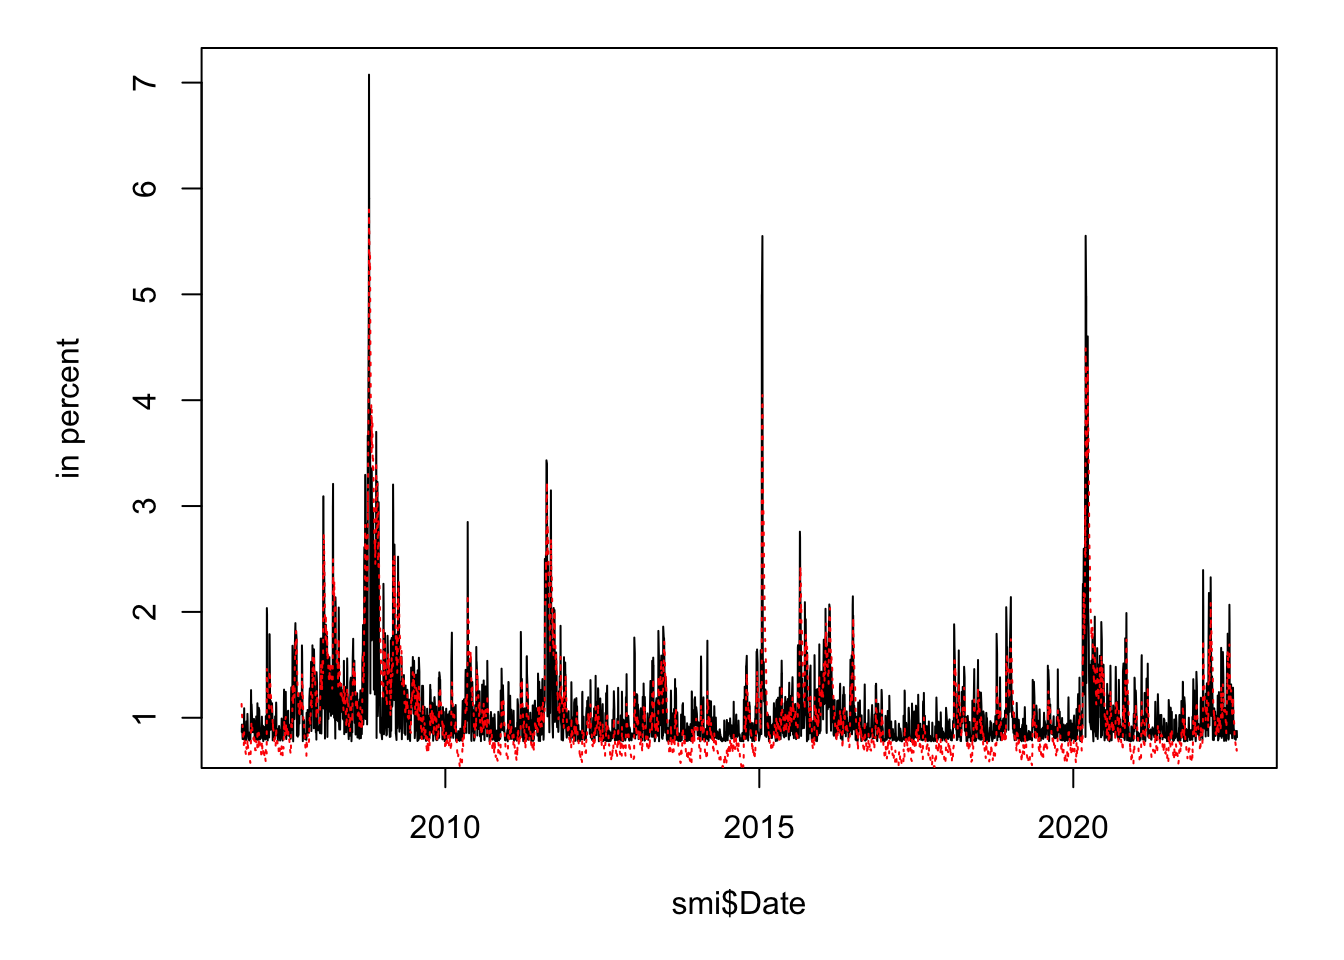
\includegraphics{TimeSeries_files/figure-latex/estimGARCH3X-1} \caption{Estimated conditional standard deviations ($\sqrt{h_t}$) of SMI daily returns: ARCH(2) [black line] and GARCH(11) [dotted red line] specifications.}\label{fig:estimGARCH3X}
\end{figure}

\hypertarget{arch-in-mean}{%
\subsection{ARCH-in-mean}\label{arch-in-mean}}

Another extension of the ARCH model is the \textbf{ARCH-in-Mean}, or ARCH-M model. That model is close to that specified by Eqs. \eqref{eq:linearreg}, \eqref{eq:uhv} and \eqref{eq:hARCH}, but it also allows for a potential effect of \(h_t\) on \(\mathbb{E}_{t-1}(y_{t})\):
\begin{eqnarray*}
y_t &=& c + \phi_1 y_{t-1} + \dots + \phi_p y_{t-p} + {\color{blue}\delta h_t}+ u_t \\
u_t &=& \sqrt{h_t} v_t \\
h_t &=& \zeta + \alpha_1 u_{t-1}^2 + \dots + \alpha_m u_{t-m}^2,
\end{eqnarray*}
where \(v_t\) is a zero-mean unit-variance i.i.d. sequence.

\hypertarget{append}{%
\chapter{Appendix}\label{append}}

\hypertarget{PCAapp}{%
\section{Principal component analysis (PCA)}\label{PCAapp}}

\textbf{Principal component analysis (PCA)} is a classical and easy-to-use statistical method to reduce the dimension of large datasets containing variables that are linearly driven by a relatively small number of factors. This approach is widely used in data analysis and image compression.

Suppose that we have \(T\) observations of a \(n\)-dimensional random vector \(x\), denoted by \(x_{1},x_{2},\ldots,x_{T}\). We suppose that each component of \(x\) is of mean zero.

Let denote with \(X\) the matrix given by \(\left[\begin{array}{cccc} x_{1} & x_{2} & \ldots & x_{T}\end{array}\right]'\). Denote the \(j^{th}\) column of \(X\) by \(X_{j}\).

We want to find the linear combination of the \(x_{i}\)'s (\(x.u\)), with \(\left\Vert u\right\Vert =1\), with ``maximum variance.'' That is, we want to solve:
\begin{equation}
\begin{array}{clll}
\underset{u}{\arg\max} & u'X'Xu. \\
\mbox{s.t. } & \left\Vert u \right\Vert =1
\end{array}\label{eq:PCA11}
\end{equation}

Since \(X'X\) is a positive definite matrix, it admits the following decomposition:
\begin{eqnarray*}
X'X & = & PDP'\\
& = & P\left[\begin{array}{ccc}
\lambda_{1}\\
& \ddots\\
&  & \lambda_{n}
\end{array}\right]P',
\end{eqnarray*}
where \(P\) is an orthogonal matrix whose columns are the eigenvectors of \(X'X\).

We can order the eigenvalues such that \(\lambda_{1}\geq\ldots\geq\lambda_{n}\). (Since \(X'X\) is positive definite, all these eigenvalues are positive.)

Since \(P\) is orthogonal, we have \(u'X'Xu=u'PDP'u=y'Dy\) where \(\left\Vert y\right\Vert =1\). Therefore, we have \(y_{i}^{2}\leq 1\) for any \(i\leq n\).

As a consequence:
\[
y'Dy=\sum_{i=1}^{n}y_{i}^{2}\lambda_{i}\leq\lambda_{1}\sum_{i=1}^{n}y_{i}^{2}=\lambda_{1}.
\]

It is easily seen that the maximum is reached for \(y=\left[1,0,\cdots,0\right]'\). Therefore, the maximum of the optimization program (Eq. \eqref{eq:PCA11}) is obtained for \(u=P\left[1,0,\cdots,0\right]'\). That is, \(u\) is the eigenvector of \(X'X\) that is associated with its larger eigenvalue (first column of \(P\)).

Let us denote with \(F\) the vector that is given by the matrix product \(XP\). The columns of \(F\), denoted by \(F_{j}\), are called \textbf{factors}. We have:
\[
F'F=P'X'XP=D.
\]
Therefore, in particular, the \(F_{j}\)'s are orthogonal.

Since \(X=FP'\), the \(X_{j}\)'s are linear combinations of the factors. Let us then denote with \(\hat{X}_{i,j}\) the part of \(X_{i}\) that is explained by factor \(F_{j}\), we have:
\begin{eqnarray*}
\hat{X}_{i,j} & = & p_{ij}F_{j}\\
X_{i} & = & \sum_{j}\hat{X}_{i,j}=\sum_{j}p_{ij}F_{j}.
\end{eqnarray*}

Consider the share of variance that is explained---through the \(n\) variables (\(X_{1},\ldots,X_{n}\))---by the first factor \(F_{1}\):
\begin{eqnarray*}
\frac{\sum_{i}\hat{X}'_{i,1}\hat{X}_{i,1}}{\sum_{i}X_{i}'X_{i}} & = & \frac{\sum_{i}p_{i1}F'_{1}F_{1}p_{i1}}{tr(X'X)} = \frac{\sum_{i}p_{i1}^{2}\lambda_{1}}{tr(X'X)} = \frac{\lambda_{1}}{\sum_{i}\lambda_{i}}.
\end{eqnarray*}

Intuitively, if the first eigenvalue is large, it means that the first factor captures a large share of the fluctutaions of the \(n\) \(X_{i}\)'s.

By the same token, it is easily seen that the fraction of the variance of the \(n\) variables that is explained by factor \(j\) is given by:
\begin{eqnarray*}
\frac{\sum_{i}\hat{X}'_{i,j}\hat{X}_{i,j}}{\sum_{i}X_{i}'X_{i}} & = & \frac{\lambda_{j}}{\sum_{i}\lambda_{i}}.
\end{eqnarray*}

Let us illustrate PCA on the term structure of yields. The term strucutre of yields (or yield curve) is know to be driven by only a small number of factors (e.g., \citet{Litterman_Scheinkman_1991}). One can typically employ PCA to recover such factors. The data used in the example below are taken from the \href{https://fred.stlouisfed.org}{Fred database} (tickers: ``DGS6MO'',``DGS1'', \ldots). The second plot shows the factor loardings, that indicate that the first factor is a level factor (loadings = black line), the second factor is a slope factor (loadings = blue line), the third factor is a curvature factor (loadings = red line).

To run a PCA, one simply has to apply function \texttt{prcomp} to a matrix of data:

\begin{Shaded}
\begin{Highlighting}[]
\FunctionTok{library}\NormalTok{(AEC)}
\NormalTok{USyields }\OtherTok{\textless{}{-}}\NormalTok{ USyields[}\FunctionTok{complete.cases}\NormalTok{(USyields),]}
\NormalTok{yds }\OtherTok{\textless{}{-}}\NormalTok{ USyields[}\FunctionTok{c}\NormalTok{(}\StringTok{"Y1"}\NormalTok{,}\StringTok{"Y2"}\NormalTok{,}\StringTok{"Y3"}\NormalTok{,}\StringTok{"Y5"}\NormalTok{,}\StringTok{"Y7"}\NormalTok{,}\StringTok{"Y10"}\NormalTok{,}\StringTok{"Y20"}\NormalTok{,}\StringTok{"Y30"}\NormalTok{)]}
\NormalTok{PCA.yds }\OtherTok{\textless{}{-}} \FunctionTok{prcomp}\NormalTok{(yds,}\AttributeTok{center=}\ConstantTok{TRUE}\NormalTok{,}\AttributeTok{scale. =} \ConstantTok{TRUE}\NormalTok{)}
\end{Highlighting}
\end{Shaded}

Let us know visualize some results. The first plot of Figure \ref{fig:USydsPCA1} shows the share of total variance explained by the different principal components (PCs). The second plot shows the factor loadings. The two bottom plots show how yields (in black) are fitted by linear combinations of the first two PCs only.

\begin{Shaded}
\begin{Highlighting}[]
\FunctionTok{par}\NormalTok{(}\AttributeTok{mfrow=}\FunctionTok{c}\NormalTok{(}\DecValTok{2}\NormalTok{,}\DecValTok{2}\NormalTok{))}
\FunctionTok{par}\NormalTok{(}\AttributeTok{plt=}\FunctionTok{c}\NormalTok{(.}\DecValTok{1}\NormalTok{,.}\DecValTok{95}\NormalTok{,.}\DecValTok{2}\NormalTok{,.}\DecValTok{8}\NormalTok{))}
\FunctionTok{barplot}\NormalTok{(PCA.yds}\SpecialCharTok{$}\NormalTok{sdev}\SpecialCharTok{\^{}}\DecValTok{2}\SpecialCharTok{/}\FunctionTok{sum}\NormalTok{(PCA.yds}\SpecialCharTok{$}\NormalTok{sdev}\SpecialCharTok{\^{}}\DecValTok{2}\NormalTok{),}
        \AttributeTok{main=}\StringTok{"Share of variance expl. by PC\textquotesingle{}s"}\NormalTok{)}
\FunctionTok{axis}\NormalTok{(}\DecValTok{1}\NormalTok{, }\AttributeTok{at=}\DecValTok{1}\SpecialCharTok{:}\FunctionTok{dim}\NormalTok{(yds)[}\DecValTok{2}\NormalTok{], }\AttributeTok{labels=}\FunctionTok{colnames}\NormalTok{(PCA.yds}\SpecialCharTok{$}\NormalTok{x))}
\NormalTok{nb.PC }\OtherTok{\textless{}{-}} \DecValTok{2}
\FunctionTok{plot}\NormalTok{(}\SpecialCharTok{{-}}\NormalTok{PCA.yds}\SpecialCharTok{$}\NormalTok{rotation[,}\DecValTok{1}\NormalTok{],}\AttributeTok{type=}\StringTok{"l"}\NormalTok{,}\AttributeTok{lwd=}\DecValTok{2}\NormalTok{,}\AttributeTok{ylim=}\FunctionTok{c}\NormalTok{(}\SpecialCharTok{{-}}\DecValTok{1}\NormalTok{,}\DecValTok{1}\NormalTok{),}
     \AttributeTok{main=}\StringTok{"Factor loadings (1st 3 PCs)"}\NormalTok{,}\AttributeTok{xaxt=}\StringTok{"n"}\NormalTok{,}\AttributeTok{xlab=}\StringTok{""}\NormalTok{)}
\FunctionTok{axis}\NormalTok{(}\DecValTok{1}\NormalTok{, }\AttributeTok{at=}\DecValTok{1}\SpecialCharTok{:}\FunctionTok{dim}\NormalTok{(yds)[}\DecValTok{2}\NormalTok{], }\AttributeTok{labels=}\FunctionTok{colnames}\NormalTok{(yds))}
\FunctionTok{lines}\NormalTok{(PCA.yds}\SpecialCharTok{$}\NormalTok{rotation[,}\DecValTok{2}\NormalTok{],}\AttributeTok{type=}\StringTok{"l"}\NormalTok{,}\AttributeTok{lwd=}\DecValTok{2}\NormalTok{,}\AttributeTok{col=}\StringTok{"blue"}\NormalTok{)}
\FunctionTok{lines}\NormalTok{(PCA.yds}\SpecialCharTok{$}\NormalTok{rotation[,}\DecValTok{3}\NormalTok{],}\AttributeTok{type=}\StringTok{"l"}\NormalTok{,}\AttributeTok{lwd=}\DecValTok{2}\NormalTok{,}\AttributeTok{col=}\StringTok{"red"}\NormalTok{)}
\NormalTok{Y1.hat }\OtherTok{\textless{}{-}}\NormalTok{ PCA.yds}\SpecialCharTok{$}\NormalTok{x[,}\DecValTok{1}\SpecialCharTok{:}\NormalTok{nb.PC] }\SpecialCharTok{\%*\%}\NormalTok{ PCA.yds}\SpecialCharTok{$}\NormalTok{rotation[}\StringTok{"Y1"}\NormalTok{,}\DecValTok{1}\SpecialCharTok{:}\DecValTok{2}\NormalTok{]}
\NormalTok{Y1.hat }\OtherTok{\textless{}{-}} \FunctionTok{mean}\NormalTok{(USyields}\SpecialCharTok{$}\NormalTok{Y1) }\SpecialCharTok{+} \FunctionTok{sd}\NormalTok{(USyields}\SpecialCharTok{$}\NormalTok{Y1) }\SpecialCharTok{*}\NormalTok{ Y1.hat}
\FunctionTok{plot}\NormalTok{(USyields}\SpecialCharTok{$}\NormalTok{date,USyields}\SpecialCharTok{$}\NormalTok{Y1,}\AttributeTok{type=}\StringTok{"l"}\NormalTok{,}\AttributeTok{lwd=}\DecValTok{2}\NormalTok{,}
     \AttributeTok{main=}\StringTok{"Fit of 1{-}year yields (2 PCs)"}\NormalTok{,}
     \AttributeTok{ylab=}\StringTok{"Obs (black) / Fitted by 2PCs (dashed blue)"}\NormalTok{)}
\FunctionTok{lines}\NormalTok{(USyields}\SpecialCharTok{$}\NormalTok{date,Y1.hat,}\AttributeTok{col=}\StringTok{"blue"}\NormalTok{,}\AttributeTok{lty=}\DecValTok{2}\NormalTok{,}\AttributeTok{lwd=}\DecValTok{2}\NormalTok{)}
\NormalTok{Y10.hat }\OtherTok{\textless{}{-}}\NormalTok{ PCA.yds}\SpecialCharTok{$}\NormalTok{x[,}\DecValTok{1}\SpecialCharTok{:}\NormalTok{nb.PC] }\SpecialCharTok{\%*\%}\NormalTok{ PCA.yds}\SpecialCharTok{$}\NormalTok{rotation[}\StringTok{"Y10"}\NormalTok{,}\DecValTok{1}\SpecialCharTok{:}\DecValTok{2}\NormalTok{]}
\NormalTok{Y10.hat }\OtherTok{\textless{}{-}} \FunctionTok{mean}\NormalTok{(USyields}\SpecialCharTok{$}\NormalTok{Y10) }\SpecialCharTok{+} \FunctionTok{sd}\NormalTok{(USyields}\SpecialCharTok{$}\NormalTok{Y10) }\SpecialCharTok{*}\NormalTok{ Y10.hat}
\FunctionTok{plot}\NormalTok{(USyields}\SpecialCharTok{$}\NormalTok{date,USyields}\SpecialCharTok{$}\NormalTok{Y10,}\AttributeTok{type=}\StringTok{"l"}\NormalTok{,}\AttributeTok{lwd=}\DecValTok{2}\NormalTok{,}
     \AttributeTok{main=}\StringTok{"Fit of 10{-}year yields (2 PCs)"}\NormalTok{,}
     \AttributeTok{ylab=}\StringTok{"Obs (black) / Fitted by 2PCs (dashed blue)"}\NormalTok{)}
\FunctionTok{lines}\NormalTok{(USyields}\SpecialCharTok{$}\NormalTok{date,Y10.hat,}\AttributeTok{col=}\StringTok{"blue"}\NormalTok{,}\AttributeTok{lty=}\DecValTok{2}\NormalTok{,}\AttributeTok{lwd=}\DecValTok{2}\NormalTok{)}
\end{Highlighting}
\end{Shaded}

\begin{figure}
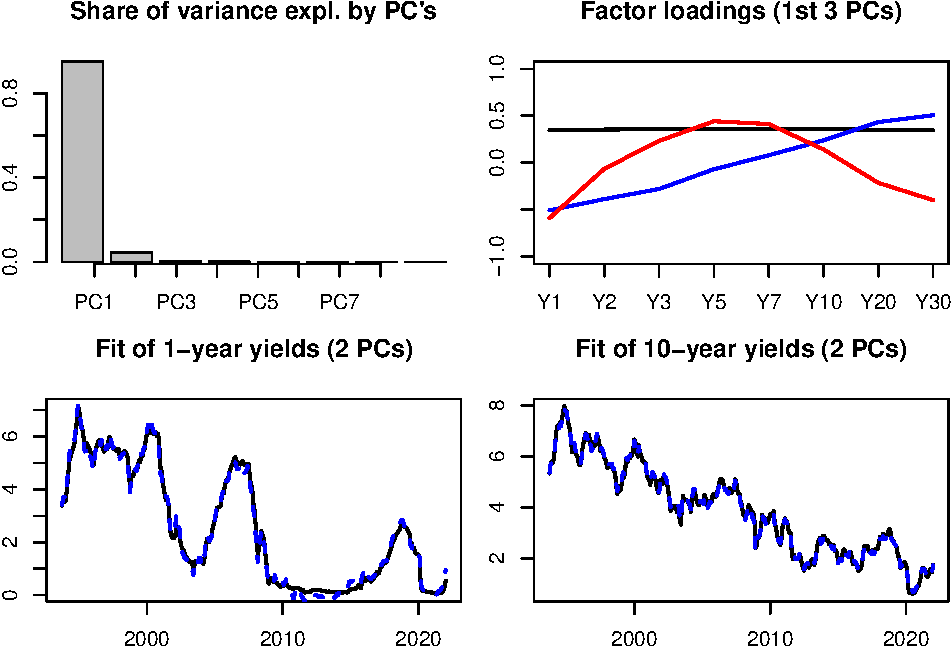
\includegraphics{TimeSeries_files/figure-latex/USydsPCA1-1} \caption{Some PCA results. The dataset contains 8 time series of U.S. interest rates of different maturities.}\label{fig:USydsPCA1}
\end{figure}

\hypertarget{LinAlgebra}{%
\section{Linear algebra: definitions and results}\label{LinAlgebra}}

\begin{definition}[Eigenvalues]
\protect\hypertarget{def:determinant}{}\label{def:determinant}The eigenvalues of of a matrix \(M\) are the numbers \(\lambda\) for which:
\[
|M - \lambda I| = 0,
\]
where \(| \bullet |\) is the determinant operator.
\end{definition}

\begin{proposition}[Properties of the determinant]
\protect\hypertarget{prp:determinant}{}\label{prp:determinant}

We have:

\begin{itemize}
\tightlist
\item
  \(|MN|=|M|\times|N|\).
\item
  \(|M^{-1}|=|M|^{-1}\).
\item
  If \(M\) admits the diagonal representation \(M=TDT^{-1}\), where \(D\) is a diagonal matrix whose diagonal entries are \(\{\lambda_i\}_{i=1,\dots,n}\), then:
  \[
  |M - \lambda I |=\prod_{i=1}^n (\lambda_i - \lambda).
  \]
\end{itemize}

\end{proposition}

\begin{definition}[Moore-Penrose inverse]
\protect\hypertarget{def:MoorPenrose}{}\label{def:MoorPenrose}

If \(M \in \mathbb{R}^{m \times n}\), then its Moore-Penrose pseudo inverse (exists and) is the unique matrix \(M^* \in \mathbb{R}^{n \times m}\) that satisfies:

\begin{enumerate}
\def\labelenumi{\roman{enumi}.}
\tightlist
\item
  \(M M^* M = M\)
\item
  \(M^* M M^* = M^*\)
\item
  \((M M^*)'=M M^*\)
  .iv \((M^* M)'=M^* M\).
\end{enumerate}

\end{definition}

\begin{proposition}[Properties of the Moore-Penrose inverse]
\protect\hypertarget{prp:MoorPenrose}{}\label{prp:MoorPenrose}

\begin{itemize}
\tightlist
\item
  If \(M\) is invertible then \(M^* = M^{-1}\).
\item
  The pseudo-inverse of a zero matrix is its transpose.
  *

  \item*

  The pseudo-inverse of the pseudo-inverse is the original matrix.
\end{itemize}

\end{proposition}

\begin{definition}[Idempotent matrix]
\protect\hypertarget{def:idempotent}{}\label{def:idempotent}Matrix \(M\) is idempotent if \(M^2=M\).

If \(M\) is a symmetric idempotent matrix, then \(M'M=M\).
\end{definition}

\begin{proposition}[Roots of an idempotent matrix]
\protect\hypertarget{prp:rootsidempotent}{}\label{prp:rootsidempotent}The eigenvalues of an idempotent matrix are either 1 or 0.
\end{proposition}

\begin{proof}
If \(\lambda\) is an eigenvalue of an idempotent matrix \(M\) then \(\exists x \ne 0\) s.t. \(Mx=\lambda x\). Hence \(M^2x=\lambda M x \Rightarrow (1-\lambda)Mx=0\). Either all element of \(Mx\) are zero, in which case \(\lambda=0\) or at least one element of \(Mx\) is nonzero, in which case \(\lambda=1\).
\end{proof}

\begin{proposition}[Idempotent matrix and chi-square distribution]
\protect\hypertarget{prp:chi2idempotent}{}\label{prp:chi2idempotent}The rank of a symmetric idempotent matrix is equal to its trace.
\end{proposition}

\begin{proof}
The result follows from Prop. \ref{prp:rootsidempotent}, combined with the fact that the rank of a symmetric matrix is equal to the number of its nonzero eigenvalues.
\end{proof}

\begin{proposition}[Constrained least squares]
\protect\hypertarget{prp:constrainedLS}{}\label{prp:constrainedLS}The solution of the following optimisation problem:
\begin{eqnarray*}
\underset{\boldsymbol\beta}{\min} && || \mathbf{y} - \mathbf{X}\boldsymbol\beta ||^2 \\
&& \mbox{subject to } \mathbf{R}\boldsymbol\beta = \mathbf{q}
\end{eqnarray*}
is given by:
\[
\boxed{\boldsymbol\beta^r = \boldsymbol\beta_0 - (\mathbf{X}'\mathbf{X})^{-1} \mathbf{R}'\{\mathbf{R}(\mathbf{X}'\mathbf{X})^{-1}\mathbf{R}'\}^{-1}(\mathbf{R}\boldsymbol\beta_0 - \mathbf{q}),}
\]
where \(\boldsymbol\beta_0=(\mathbf{X}'\mathbf{X})^{-1}\mathbf{X}'\mathbf{y}\).
\end{proposition}

\begin{proof}
See for instance \href{http://jackman.stanford.edu/classes/350B/07/ftestforWeb.pdf}{Jackman, 2007}.
\end{proof}

\begin{proposition}[Inverse of a partitioned matrix]
\protect\hypertarget{prp:inversepartitioned}{}\label{prp:inversepartitioned}We have:
\begin{eqnarray*}
&&\left[ \begin{array}{cc} \mathbf{A}_{11} & \mathbf{A}_{12} \\ \mathbf{A}_{21} & \mathbf{A}_{22} \end{array}\right]^{-1} = \\
&&\left[ \begin{array}{cc} (\mathbf{A}_{11} - \mathbf{A}_{12}\mathbf{A}_{22}^{-1}\mathbf{A}_{21})^{-1} & - \mathbf{A}_{11}^{-1}\mathbf{A}_{12}(\mathbf{A}_{22} - \mathbf{A}_{21}\mathbf{A}_{11}^{-1}\mathbf{A}_{12})^{-1} \\
-(\mathbf{A}_{22} - \mathbf{A}_{21}\mathbf{A}_{11}^{-1}\mathbf{A}_{12})^{-1}\mathbf{A}_{21}\mathbf{A}_{11}^{-1} & (\mathbf{A}_{22} - \mathbf{A}_{21}\mathbf{A}_{11}^{-1}\mathbf{A}_{12})^{-1} \end{array} \right].
\end{eqnarray*}
\end{proposition}

\begin{definition}[Matrix derivatives]
\protect\hypertarget{def:FOD}{}\label{def:FOD}Consider a fonction \(f: \mathbb{R}^K \rightarrow \mathbb{R}\). Its first-order derivative is:
\[
\frac{\partial f}{\partial \mathbf{b}}(\mathbf{b}) =
\left[\begin{array}{c}
\frac{\partial f}{\partial b_1}(\mathbf{b})\\
\vdots\\
\frac{\partial f}{\partial b_K}(\mathbf{b})
\end{array}
\right].
\]
We use the notation:
\[
\frac{\partial f}{\partial \mathbf{b}'}(\mathbf{b}) = \left(\frac{\partial f}{\partial \mathbf{b}}(\mathbf{b})\right)'.
\]
\end{definition}

\begin{proposition}
\protect\hypertarget{prp:partial}{}\label{prp:partial}

We have:

\begin{itemize}
\tightlist
\item
  If \(f(\mathbf{b}) = A' \mathbf{b}\) where \(A\) is a \(K \times 1\) vector then \(\frac{\partial f}{\partial \mathbf{b}}(\mathbf{b}) = A\).
\item
  If \(f(\mathbf{b}) = \mathbf{b}'A\mathbf{b}\) where \(A\) is a \(K \times K\) matrix, then \(\frac{\partial f}{\partial \mathbf{b}}(\mathbf{b}) = 2A\mathbf{b}\).
\end{itemize}

\end{proposition}

\begin{proposition}[Square and absolute summability]
\protect\hypertarget{prp:absMs}{}\label{prp:absMs}We have:
\[
\underbrace{\sum_{i=0}^{\infty}|\theta_i| < + \infty}_{\mbox{Absolute summability}} \Rightarrow \underbrace{\sum_{i=0}^{\infty} \theta_i^2 < + \infty}_{\mbox{Square summability}}.
\]
\end{proposition}

\begin{proof}
See Appendix 3.A in Hamilton. Idea: Absolute summability implies that there exist \(N\) such that, for \(j>N\), \(|\theta_j| < 1\) (deduced from Cauchy criterion, Theorem \ref{thm:cauchycritstatic} and therefore \(\theta_j^2 < |\theta_j|\).
\end{proof}

\hypertarget{variousResults}{%
\section{Statistical analysis: definitions and results}\label{variousResults}}

\hypertarget{moments-and-statistics}{%
\subsection{Moments and statistics}\label{moments-and-statistics}}

\begin{definition}[Partial correlation]
\protect\hypertarget{def:partialcorrel}{}\label{def:partialcorrel}The \textbf{partial correlation} between \(y\) and \(z\), controlling for some variables \(\mathbf{X}\) is the sample correlation between \(y^*\) and \(z^*\), where the latter two variables are the residuals in regressions of \(y\) on \(\mathbf{X}\) and of \(z\) on \(\mathbf{X}\), respectively.

This correlation is denoted by \(r_{yz}^\mathbf{X}\). By definition, we have:
\begin{equation}
r_{yz}^\mathbf{X} = \frac{\mathbf{z^*}'\mathbf{y^*}}{\sqrt{(\mathbf{z^*}'\mathbf{z^*})(\mathbf{y^*}'\mathbf{y^*})}}.\label{eq:pc}
\end{equation}
\end{definition}

\begin{definition}[Skewness and kurtosis]
\protect\hypertarget{def:skewnesskurtosis}{}\label{def:skewnesskurtosis}

Let \(Y\) be a random variable whose fourth moment exists. The expectation of \(Y\) is denoted by \(\mu\).

\begin{itemize}
\tightlist
\item
  The skewness of \(Y\) is given by:
  \[
  \frac{\mathbb{E}[(Y-\mu)^3]}{\{\mathbb{E}[(Y-\mu)^2]\}^{3/2}}.
  \]
\item
  The kurtosis of \(Y\) is given by:
  \[
  \frac{\mathbb{E}[(Y-\mu)^4]}{\{\mathbb{E}[(Y-\mu)^2]\}^{2}}.
  \]
\end{itemize}

\end{definition}

\begin{theorem}[Cauchy-Schwarz inequality]
\protect\hypertarget{thm:CauchySchwarz}{}\label{thm:CauchySchwarz}We have:
\[
|\mathbb{C}ov(X,Y)| \le \sqrt{\mathbb{V}ar(X)\mathbb{V}ar(Y)}
\]
and, if \(X \ne =\) and \(Y \ne 0\), the equality holds iff \(X\) and \(Y\) are the same up to an affine transformation.
\end{theorem}

\begin{proof}
If \(\mathbb{V}ar(X)=0\), this is trivial. If this is not the case, then let's define \(Z\) as \(Z = Y - \frac{\mathbb{C}ov(X,Y)}{\mathbb{V}ar(X)}X\). It is easily seen that \(\mathbb{C}ov(X,Z)=0\). Then, the variance of \(Y=Z+\frac{\mathbb{C}ov(X,Y)}{\mathbb{V}ar(X)}X\) is equal to the sum of the variance of \(Z\) and of the variance of \(\frac{\mathbb{C}ov(X,Y)}{\mathbb{V}ar(X)}X\), that is:
\[
\mathbb{V}ar(Y) = \mathbb{V}ar(Z) + \left(\frac{\mathbb{C}ov(X,Y)}{\mathbb{V}ar(X)}\right)^2\mathbb{V}ar(X) \ge \left(\frac{\mathbb{C}ov(X,Y)}{\mathbb{V}ar(X)}\right)^2\mathbb{V}ar(X).
\]
The equality holds iff \(\mathbb{V}ar(Z)=0\), i.e.~iff \(Y = \frac{\mathbb{C}ov(X,Y)}{\mathbb{V}ar(X)}X+cst\).
\end{proof}

\begin{definition}[Mean ergodicity]
\protect\hypertarget{def:ergodicity}{}\label{def:ergodicity}The covariance-stationary process \(y_t\) is ergodic for the mean if:
\[
\mbox{plim}_{T \rightarrow +\infty} \frac{1}{T}\sum_{t=1}^T y_t = \mathbb{E}(y_t).
\]
\end{definition}

\begin{definition}[Second-moment ergodicity]
\protect\hypertarget{def:ergod2nd}{}\label{def:ergod2nd}The covariance-stationary process \(y_t\) is ergodic for second moments if, for all \(j\):
\[
\mbox{plim}_{T \rightarrow +\infty} \frac{1}{T}\sum_{t=1}^T (y_t-\mu) (y_{t-j}-\mu) = \gamma_j.
\]
\end{definition}

It should be noted that ergodicity and stationarity are different properties. Typically if the process \(\{x_t\}\) is such that, \(\forall t\), \(x_t \equiv y\), where \(y \sim\,\mathcal{N}(0,1)\) (say), then \(\{x_t\}\) is stationary but not ergodic.

\hypertarget{standard-distributions}{%
\subsection{Standard distributions}\label{standard-distributions}}

\begin{definition}[F distribution]
\protect\hypertarget{def:fstatistics}{}\label{def:fstatistics}Consider \(n=n_1+n_2\) i.i.d. \(\mathcal{N}(0,1)\) r.v. \(X_i\). If the r.v. \(F\) is defined by:
\[
F = \frac{\sum_{i=1}^{n_1} X_i^2}{\sum_{j=n_1+1}^{n_1+n_2} X_j^2}\frac{n_2}{n_1}
\]
then \(F \sim \mathcal{F}(n_1,n_2)\). (See Table \ref{tab:Fstat} for quantiles.)
\end{definition}

\begin{definition}[Student-t distribution]
\protect\hypertarget{def:tStudent}{}\label{def:tStudent}\(Z\) follows a Student-t (or \(t\)) distribution with \(\nu\) degrees of freedom (d.f.) if:
\[
Z = X_0 \bigg/ \sqrt{\frac{\sum_{i=1}^{\nu}X_i^2}{\nu}}, \quad X_i \sim i.i.d. \mathcal{N}(0,1).
\]
We have \(\mathbb{E}(Z)=0\), and \(\mathbb{V}ar(Z)=\frac{\nu}{\nu-2}\) if \(\nu>2\). (See Table \ref{tab:Student} for quantiles.)
\end{definition}

\begin{definition}[Chi-square distribution]
\protect\hypertarget{def:chi2}{}\label{def:chi2}\(Z\) follows a \(\chi^2\) distribution with \(\nu\) d.f. if \(Z = \sum_{i=1}^{\nu}X_i^2\) where \(X_i \sim i.i.d. \mathcal{N}(0,1)\).
We have \(\mathbb{E}(Z)=\nu\). (See Table \ref{tab:Chi2} for quantiles.)
\end{definition}

\begin{definition}[Cauchy distribution]
\protect\hypertarget{def:Cauchy}{}\label{def:Cauchy}

The probability distribution function of the Cauchy distribution defined by a location parameter \(\mu\) and a scale parameter \(\gamma\) is:
\[
f(x) = \frac{1}{\pi \gamma \left(1 + \left[\frac{x-\mu}{\gamma}\right]^2\right)}.
\]
The mean and variance of this distribution are undefined.

\begin{figure}
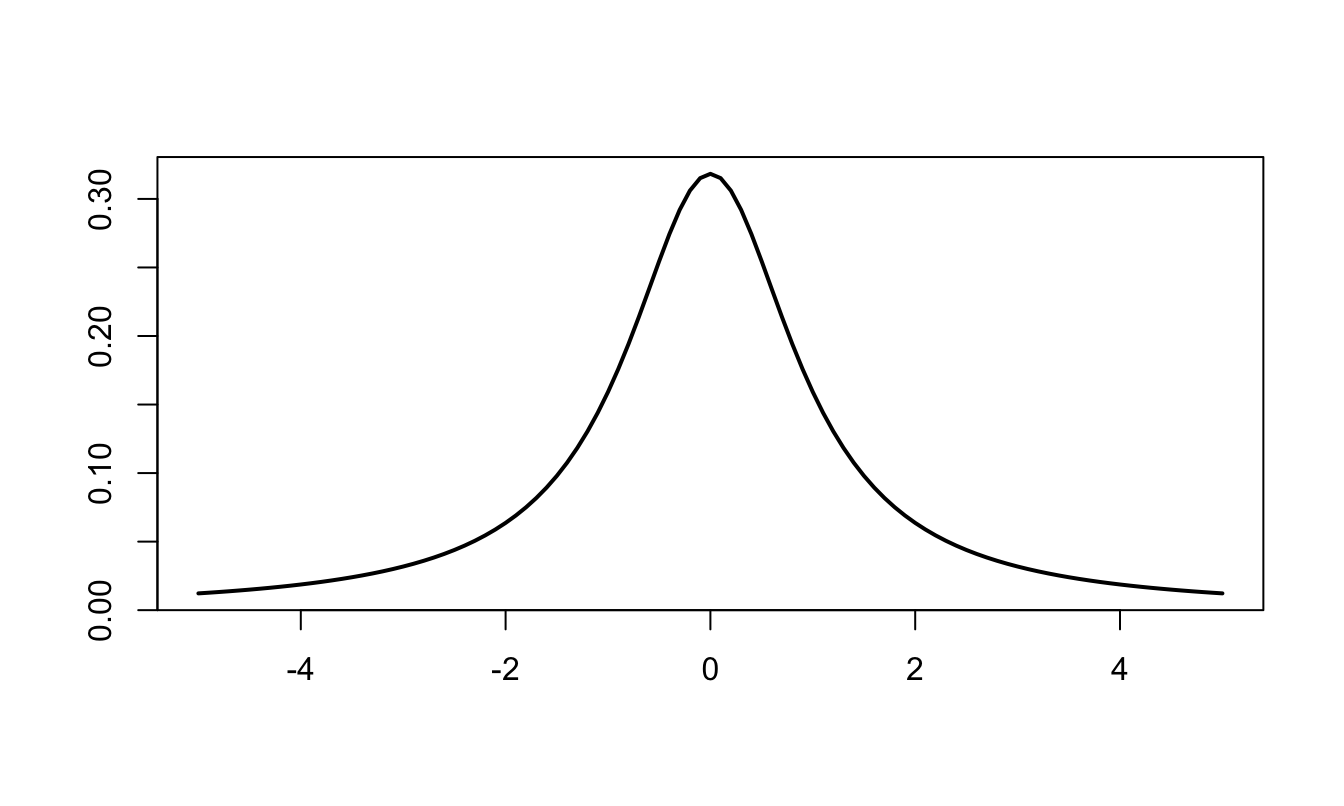
\includegraphics[width=0.95\linewidth]{TimeSeries_files/figure-latex/Cauchy-1} \caption{Pdf of the Cauchy distribution ($\mu=0$, $\gamma=1$).}\label{fig:Cauchy}
\end{figure}

\end{definition}

\begin{proposition}[Inner product of a multivariate Gaussian variable]
\protect\hypertarget{prp:waldtypeproduct}{}\label{prp:waldtypeproduct}Let \(X\) be a \(n\)-dimensional multivariate Gaussian variable: \(X \sim \mathcal{N}(0,\Sigma)\). We have:
\[
X' \Sigma^{-1}X \sim \chi^2(n).
\]
\end{proposition}

\begin{proof}
Because \(\Sigma\) is a symmetrical definite positive matrix, it admits the spectral decomposition \(PDP'\) where \(P\) is an orthogonal matrix (i.e.~\(PP'=Id\)) and D is a diagonal matrix with non-negative entries. Denoting by \(\sqrt{D^{-1}}\) the diagonal matrix whose diagonal entries are the inverse of those of \(D\), it is easily checked that the covariance matrix of \(Y:=\sqrt{D^{-1}}P'X\) is \(Id\). Therefore \(Y\) is a vector of uncorrelated Gaussian variables. The properties of Gaussian variables imply that the components of \(Y\) are then also independent. Hence \(Y'Y=\sum_i Y_i^2 \sim \chi^2(n)\).

It remains to note that \(Y'Y=X'PD^{-1}P'X=X'\mathbb{V}ar(X)^{-1}X\) to conclude.
\end{proof}

\hypertarget{StochConvergences}{%
\subsection{Stochastic convergences}\label{StochConvergences}}

\begin{definition}[Convergence in probability]
\protect\hypertarget{def:convergenceproba}{}\label{def:convergenceproba}The random variable sequence \(x_n\) converges in probability to a constant \(c\) if \(\forall \varepsilon\), \(\lim_{n \rightarrow \infty} \mathbb{P}(|x_n - c|>\varepsilon) = 0\).

It is denoted as: \(\mbox{plim } x_n = c\).
\end{definition}

\begin{definition}[Convergence in the Lr norm]
\protect\hypertarget{def:convergenceLr}{}\label{def:convergenceLr}\(x_n\) converges in the \(r\)-th mean (or in the \(L^r\)-norm) towards \(x\), if \(\mathbb{E}(|x_n|^r)\) and \(\mathbb{E}(|x|^r)\) exist and if
\[
\lim_{n \rightarrow \infty} \mathbb{E}(|x_n - x|^r) = 0.
\]
It is denoted as: \(x_n \overset{L^r}{\rightarrow} c\).

For \(r=2\), this convergence is called \textbf{mean square convergence}.
\end{definition}

\begin{definition}[Almost sure convergence]
\protect\hypertarget{def:convergenceAlmost}{}\label{def:convergenceAlmost}The random variable sequence \(x_n\) converges almost surely to \(c\) if \(\mathbb{P}(\lim_{n \rightarrow \infty} x_n = c) = 1\).

It is denoted as: \(x_n \overset{a.s.}{\rightarrow} c\).
\end{definition}

\begin{definition}[Convergence in distribution]
\protect\hypertarget{def:cvgceDistri}{}\label{def:cvgceDistri}\(x_n\) is said to converge in distribution (or in law) to \(x\) if
\[
\lim_{n \rightarrow \infty} F_{x_n}(s) = F_{x}(s)
\]
for all \(s\) at which \(F_X\) --the cumulative distribution of \(X\)-- is continuous.

It is denoted as: \(x_n \overset{d}{\rightarrow} x\).
\end{definition}

\begin{theorem}[Cauchy criterion (non-stochastic case)]
\protect\hypertarget{thm:cauchycritstatic}{}\label{thm:cauchycritstatic}We have that \(\sum_{i=0}^{T} a_i\) converges (\(T \rightarrow \infty\)) iff, for any \(\eta > 0\), there exists an integer \(N\) such that, for all \(M\ge N\),
\[
\left|\sum_{i=N+1}^{M} a_i\right| < \eta.
\]
\end{theorem}

\begin{theorem}[Cauchy criterion (stochastic case)]
\protect\hypertarget{thm:cauchycritstochastic}{}\label{thm:cauchycritstochastic}We have that \(\sum_{i=0}^{T} \theta_i \varepsilon_{t-i}\) converges in mean square (\(T \rightarrow \infty\)) to a random variable iff, for any \(\eta > 0\), there exists an integer \(N\) such that, for all \(M\ge N\),
\[
\mathbb{E}\left[\left(\sum_{i=N+1}^{M} \theta_i \varepsilon_{t-i}\right)^2\right] < \eta.
\]
\end{theorem}

\hypertarget{multivariate-gaussian-distribution}{%
\subsection{Multivariate Gaussian distribution}\label{multivariate-gaussian-distribution}}

\begin{proposition}[p.d.f. of a multivariate Gaussian variable]
\protect\hypertarget{prp:pdfMultivarGaussian}{}\label{prp:pdfMultivarGaussian}If \(Y \sim \mathcal{N}(\mu,\Omega)\) and if \(Y\) is a \(n\)-dimensional vector, then the density function of \(Y\) is:
\[
\frac{1}{(2 \pi)^{n/2}|\Omega|^{1/2}}\exp\left[-\frac{1}{2}\left(Y-\mu\right)'\Omega^{-1}\left(Y-\mu\right)\right].
\]
\end{proposition}

\hypertarget{CLTappend}{%
\subsection{Central limit theorem}\label{CLTappend}}

\begin{theorem}[Law of large numbers]
\protect\hypertarget{thm:LLNappendix}{}\label{thm:LLNappendix}The sample mean is a consistent estimator of the population mean.
\end{theorem}

\begin{proof}
Let's denote by \(\phi_{X_i}\) the characteristic function of a r.v. \(X_i\). If the mean of \(X_i\) is \(\mu\) then the Talyor expansion of the characteristic function is:
\[
\phi_{X_i}(u) = \mathbb{E}(\exp(iuX)) = 1 + iu\mu + o(u).
\]
The properties of the characteristic function (see Def. \ref{def:characteristic}) imply that:
\[
\phi_{\frac{1}{n}(X_1+\dots+X_n)}(u) = \prod_{i=1}^{n} \left(1 + i\frac{u}{n}\mu + o\left(\frac{u}{n}\right) \right) \rightarrow e^{iu\mu}.
\]
The facts that (a) \(e^{iu\mu}\) is the characteristic function of the constant \(\mu\) and (b) that a characteristic function uniquely characterises a distribution imply that the sample mean converges in distribution to the constant \(\mu\), which further implies that it converges in probability to \(\mu\).
\end{proof}

\begin{theorem}[Lindberg-Levy Central limit theorem, CLT]
\protect\hypertarget{thm:LindbergLevyCLT}{}\label{thm:LindbergLevyCLT}If \(x_n\) is an i.i.d. sequence of random variables with mean \(\mu\) and variance \(\sigma^2\) (\(\in ]0,+\infty[\)), then:
\[
\boxed{\sqrt{n} (\bar{x}_n - \mu) \overset{d}{\rightarrow} \mathcal{N}(0,\sigma^2), \quad \mbox{where} \quad \bar{x}_n = \frac{1}{n} \sum_{i=1}^{n} x_i.}
\]
\end{theorem}

\begin{proof}
Let us introduce the r.v. \(Y_n:= \sqrt{n}(\bar{X}_n - \mu)\). We have \(\phi_{Y_n}(u) = \left[ \mathbb{E}\left( \exp(i \frac{1}{\sqrt{n}} u (X_1 - \mu)) \right) \right]^n\). We have:
\begin{eqnarray*}
&&\left[ \mathbb{E}\left( \exp\left(i \frac{1}{\sqrt{n}} u (X_1 - \mu)\right) \right) \right]^n\\
&=& \left[ \mathbb{E}\left( 1 + i \frac{1}{\sqrt{n}} u (X_1 - \mu) - \frac{1}{2n} u^2 (X_1 - \mu)^2 + o(u^2) \right) \right]^n \\
&=& \left( 1 - \frac{1}{2n}u^2\sigma^2 + o(u^2)\right)^n.
\end{eqnarray*}
Therefore \(\phi_{Y_n}(u) \underset{n \rightarrow \infty}{\rightarrow} \exp \left( - \frac{1}{2}u^2\sigma^2 \right)\), which is the characteristic function of \(\mathcal{N}(0,\sigma^2)\).
\end{proof}

\hypertarget{AppendixProof}{%
\section{Proofs}\label{AppendixProof}}

\textbf{Proof of Eq. \eqref{eq:TCL2}}

\begin{proof}
We have:
\begin{eqnarray*}
&&T\mathbb{E}\left[(\bar{y}_T - \mu)^2\right]\\
&=& T\mathbb{E}\left[\left(\frac{1}{T}\sum_{t=1}^T(y_t - \mu)\right)^2\right] = \frac{1}{T} \mathbb{E}\left[\sum_{t=1}^T(y_t - \mu)^2+2\sum_{s<t\le T}(y_t - \mu)(y_s - \mu)\right]\\
&=& \gamma_0 +\frac{2}{T}\left(\sum_{t=2}^{T}\mathbb{E}\left[(y_t - \mu)(y_{t-1} - \mu)\right]\right) +\frac{2}{T}\left(\sum_{t=3}^{T}\mathbb{E}\left[(y_t - \mu)(y_{t-2} - \mu)\right]\right) + \dots \\
&&+ \frac{2}{T}\left(\sum_{t=T-1}^{T}\mathbb{E}\left[(y_t - \mu)(y_{t-(T-2)} - \mu)\right]\right) + \frac{2}{T}\mathbb{E}\left[(y_t - \mu)(y_{t-(T-1)} - \mu)\right]\\
&=&  \gamma_0 + 2 \frac{T-1}{T}\gamma_1 + \dots + 2 \frac{1}{T}\gamma_{T-1} .
\end{eqnarray*}
Therefore:
\begin{eqnarray*}
&& T\mathbb{E}\left[(\bar{y}_T - \mu)^2\right] - \sum_{j=-\infty}^{+\infty} \gamma_j \\
&=& - 2\frac{1}{T}\gamma_1 - 2\frac{2}{T}\gamma_2 - \dots - 2\frac{T-1}{T}\gamma_{T-1} - 2\gamma_T - 2 \gamma_{T+1} + \dots
\end{eqnarray*}
And then:
\begin{eqnarray*}
&& \left|T\mathbb{E}\left[(\bar{y}_T - \mu)^2\right] - \sum_{j=-\infty}^{+\infty} \gamma_j\right|\\
&\le& 2\frac{1}{T}|\gamma_1| + 2\frac{2}{T}|\gamma_2| + \dots + 2\frac{T-1}{T}|\gamma_{T-1}| + 2|\gamma_T| + 2 |\gamma_{T+1}| + \dots
\end{eqnarray*}

For any \(q \le T\), we have:
\begin{eqnarray*}
\left|T\mathbb{E}\left[(\bar{y}_T - \mu)^2\right] - \sum_{j=-\infty}^{+\infty} \gamma_j\right| &\le& 2\frac{1}{T}|\gamma_1| + 2\frac{2}{T}|\gamma_2| + \dots + 2\frac{q-1}{T}|\gamma_{q-1}| +2\frac{q}{T}|\gamma_q| +\\
&&2\frac{q+1}{T}|\gamma_{q+1}| + \dots  + 2\frac{T-1}{T}|\gamma_{T-1}| + 2|\gamma_T| + 2 |\gamma_{T+1}| + \dots\\
&\le& \frac{2}{T}\left(|\gamma_1| + 2|\gamma_2| + \dots + (q-1)|\gamma_{q-1}| +q|\gamma_q|\right) +\\
&&2|\gamma_{q+1}| + \dots  + 2|\gamma_{T-1}| + 2|\gamma_T| + 2 |\gamma_{T+1}| + \dots
\end{eqnarray*}

Consider \(\varepsilon > 0\). The fact that the autocovariances are absolutely summable implies that there exists \(q_0\) such that (Cauchy criterion, Theorem \ref{thm:cauchycritstatic}):
\[
2|\gamma_{q_0+1}|+2|\gamma_{q_0+2}|+2|\gamma_{q_0+3}|+\dots < \varepsilon/2.
\]
Then, if \(T > q_0\), it comes that:
\[
\left|T \mathbb{E}\left[(\bar{y}_T - \mu)^2\right] - \sum_{j=-\infty}^{+\infty} \gamma_j\right|\le \frac{2}{T}\left(|\gamma_1| + 2|\gamma_2| + \dots + (q_0-1)|\gamma_{q_0-1}| +q_0|\gamma_{q_0}|\right) + \varepsilon/2.
\]
If \(T \ge 2\left(|\gamma_1| + 2|\gamma_2| + \dots + (q_0-1)|\gamma_{q_0-1}| +q_0|\gamma_{q_0}|\right)/(\varepsilon/2)\) (\(= f(q_0)\), say) then
\[
\frac{2}{T}\left(|\gamma_1| + 2|\gamma_2| + \dots + (q_0-1)|\gamma_{q_0-1}| +q_0|\gamma_{q_0}|\right) \le \varepsilon/2.
\]
Then, if \(T>f(q_0)\) and \(T>q_0\), i.e.~if \(T>\max(f(q_0),q_0)\), we have:
\[
\left|T \mathbb{E}\left[(\bar{y}_T - \mu)^2\right] - \sum_{j=-\infty}^{+\infty} \gamma_j\right|\le \varepsilon.
\]
\end{proof}

\textbf{Proof of Proposition \ref{prp:smallestMSE}}

\begin{proof}
We have:
\begin{eqnarray}
\mathbb{E}([y_{t+1} - y^*_{t+1}]^2) &=& \mathbb{E}\left([\color{blue}{\{y_{t+1} - \mathbb{E}(y_{t+1}|x_t)\}} + \color{red}{\{\mathbb{E}(y_{t+1}|x_t)  - y^*_{t+1}\}}]^2\right)\nonumber\\
&=&  \mathbb{E}\left(\color{blue}{[y_{t+1} - \mathbb{E}(y_{t+1}|x_t)]}^2\right) + \mathbb{E}\left(\color{red}{[\mathbb{E}(y_{t+1}|x_t)  - y^*_{t+1}]}^2\right)\nonumber\\
&& + 2\mathbb{E}\left( \color{blue}{[y_{t+1} - \mathbb{E}(y_{t+1}|x_t)]}\color{red}{ [\mathbb{E}(y_{t+1}|x_t)  - y^*_{t+1}]}\right). \label{eq:1}
\end{eqnarray}
Let us focus on the last term. We have:
\begin{eqnarray*}
&&\mathbb{E}\left(\color{blue}{[y_{t+1} - \mathbb{E}(y_{t+1}|x_t)]}\color{red}{ [\mathbb{E}(y_{t+1}|x_t)  - y^*_{t+1}]}\right)\\
&=& \mathbb{E}( \mathbb{E}( \color{blue}{[y_{t+1} - \mathbb{E}(y_{t+1}|x_t)]}\color{red}{ \underbrace{[\mathbb{E}(y_{t+1}|x_t)  - y^*_{t+1}]}_{\mbox{function of $x_t$}}}|x_t))\\
&=& \mathbb{E}( \color{red}{ [\mathbb{E}(y_{t+1}|x_t)  - y^*_{t+1}]} \mathbb{E}( \color{blue}{[y_{t+1} - \mathbb{E}(y_{t+1}|x_t)]}|x_t))\\
&=& \mathbb{E}( \color{red}{ [\mathbb{E}(y_{t+1}|x_t)  - y^*_{t+1}]} \color{blue}{\underbrace{[\mathbb{E}(y_{t+1}|x_t) - \mathbb{E}(y_{t+1}|x_t)]}_{=0}})=0.
\end{eqnarray*}

Therefore, Eq. \eqref{eq:1} becomes:
\begin{eqnarray*}
&&\mathbb{E}([y_{t+1} - y^*_{t+1}]^2) \\
&=&  \underbrace{\mathbb{E}\left(\color{blue}{[y_{t+1} - \mathbb{E}(y_{t+1}|x_t)]}^2\right)}_{\mbox{$\ge 0$ and does not depend on $y^*_{t+1}$}} + \underbrace{\mathbb{E}\left(\color{red}{[\mathbb{E}(y_{t+1}|x_t)  - y^*_{t+1}]}^2\right)}_{\mbox{$\ge 0$ and depends on $y^*_{t+1}$}}.
\end{eqnarray*}
This implies that \(\mathbb{E}([y_{t+1} - y^*_{t+1}]^2)\) is always larger than \(\color{blue}{\mathbb{E}([y_{t+1} - \mathbb{E}(y_{t+1}|x_t)]^2)}\), and is therefore minimized if the second term is equal to zero, that is if \(\mathbb{E}(y_{t+1}|x_t) = y^*_{t+1}\).
\end{proof}

\textbf{Proof of Proposition \ref{prp:estimVARGaussian}}

\begin{proof}
Using Proposition \ref{prp:multivarG}, we obtain that, conditionally on \(x_1\), the log-likelihood is given by
\begin{eqnarray*}
\log\mathcal{L}(Y_{T};\theta) & = & -(Tn/2)\log(2\pi)+(T/2)\log\left|\Omega^{-1}\right|\\
&  & -\frac{1}{2}\sum_{t=1}^{T}\left[\left(y_{t}-\Pi'x_{t}\right)'\Omega^{-1}\left(y_{t}-\Pi'x_{t}\right)\right].
\end{eqnarray*}
Let's rewrite the last term of the log-likelihood:
\begin{eqnarray*}
\sum_{t=1}^{T}\left[\left(y_{t}-\Pi'x_{t}\right)'\Omega^{-1}\left(y_{t}-\Pi'x_{t}\right)\right] & =\\
\sum_{t=1}^{T}\left[\left(y_{t}-\hat{\Pi}'x_{t}+\hat{\Pi}'x_{t}-\Pi'x_{t}\right)'\Omega^{-1}\left(y_{t}-\hat{\Pi}'x_{t}+\hat{\Pi}'x_{t}-\Pi'x_{t}\right)\right] & =\\
\sum_{t=1}^{T}\left[\left(\hat{\varepsilon}_{t}+(\hat{\Pi}-\Pi)'x_{t}\right)'\Omega^{-1}\left(\hat{\varepsilon}_{t}+(\hat{\Pi}-\Pi)'x_{t}\right)\right],
\end{eqnarray*}
where the \(j^{th}\) element of the \((n\times1)\) vector \(\hat{\varepsilon}_{t}\) is the sample residual, for observation \(t\), from an OLS regression of \(y_{j,t}\) on \(x_{t}\). Expanding the previous equation, we get:
\begin{eqnarray*}
&&\sum_{t=1}^{T}\left[\left(y_{t}-\Pi'x_{t}\right)'\Omega^{-1}\left(y_{t}-\Pi'x_{t}\right)\right]  = \sum_{t=1}^{T}\hat{\varepsilon}_{t}'\Omega^{-1}\hat{\varepsilon}_{t}\\
&&+2\sum_{t=1}^{T}\hat{\varepsilon}_{t}'\Omega^{-1}(\hat{\Pi}-\Pi)'x_{t}+\sum_{t=1}^{T}x'_{t}(\hat{\Pi}-\Pi)\Omega^{-1}(\hat{\Pi}-\Pi)'x_{t}.
\end{eqnarray*}
Let's apply the trace operator on the second term (that is a scalar):
\begin{eqnarray*}
\sum_{t=1}^{T}\hat{\varepsilon}_{t}'\Omega^{-1}(\hat{\Pi}-\Pi)'x_{t} & = & Tr\left(\sum_{t=1}^{T}\hat{\varepsilon}_{t}'\Omega^{-1}(\hat{\Pi}-\Pi)'x_{t}\right)\\
=  Tr\left(\sum_{t=1}^{T}\Omega^{-1}(\hat{\Pi}-\Pi)'x_{t}\hat{\varepsilon}_{t}'\right) & = & Tr\left(\Omega^{-1}(\hat{\Pi}-\Pi)'\sum_{t=1}^{T}x_{t}\hat{\varepsilon}_{t}'\right).
\end{eqnarray*}
Given that, by construction (property of OLS estimates), the sample residuals are orthogonal to the explanatory variables, this term is zero. Introducing \(\tilde{x}_{t}=(\hat{\Pi}-\Pi)'x_{t}\), we have
\begin{eqnarray*}
\sum_{t=1}^{T}\left[\left(y_{t}-\Pi'x_{t}\right)'\Omega^{-1}\left(y_{t}-\Pi'x_{t}\right)\right] =\sum_{t=1}^{T}\hat{\varepsilon}_{t}'\Omega^{-1}\hat{\varepsilon}_{t}+\sum_{t=1}^{T}\tilde{x}'_{t}\Omega^{-1}\tilde{x}_{t}.
\end{eqnarray*}
Since \(\Omega\) is a positive definite matrix, \(\Omega^{-1}\) is as well. Consequently, the smallest value that the last term can take is obtained for \(\tilde{x}_{t}=0\), i.e.~when \(\Pi=\hat{\Pi}.\)

The MLE of \(\Omega\) is the matrix \(\hat{\Omega}\) that maximizes \(\Omega\overset{\ell}{\rightarrow}L(Y_{T};\hat{\Pi},\Omega)\). We have:
\begin{eqnarray*}
\log\mathcal{L}(Y_{T};\hat{\Pi},\Omega) & = & -(Tn/2)\log(2\pi)+(T/2)\log\left|\Omega^{-1}\right| -\frac{1}{2}\sum_{t=1}^{T}\left[\hat{\varepsilon}_{t}'\Omega^{-1}\hat{\varepsilon}_{t}\right].
\end{eqnarray*}

Matrix \(\hat{\Omega}\) is a symmetric positive definite. It is easily checked that the (unrestricted) matrix that maximizes the latter expression is symmetric positive definite matrix. Indeed:
\[
\frac{\partial \log\mathcal{L}(Y_{T};\hat{\Pi},\Omega)}{\partial\Omega}=\frac{T}{2}\Omega'-\frac{1}{2}\sum_{t=1}^{T}\hat{\varepsilon}_{t}\hat{\varepsilon}'_{t}\Rightarrow\hat{\Omega}'=\frac{1}{T}\sum_{t=1}^{T}\hat{\varepsilon}_{t}\hat{\varepsilon}'_{t},
\]
which leads to the result.
\end{proof}

\textbf{Proof of Proposition \ref{prp:OLSVAR}}

\begin{proof}
Let us drop the \(i\) subscript. Rearranging Eq. \eqref{eq:olsar1}, we have:
\[
\sqrt{T}(\mathbf{b}-\boldsymbol{\beta}) =  (X'X/T)^{-1}\sqrt{T}(X'\boldsymbol\varepsilon/T).
\]
Let us consider the autocovariances of \(\mathbf{v}_t = x_t \varepsilon_t\), denoted by \(\gamma^v_j\). Using the fact that \(x_t\) is a linear combination of past \(\varepsilon_t\)s and that \(\varepsilon_t\) is a white noise, we get that \(\mathbb{E}(\varepsilon_t x_t)=0\). Therefore
\[
\gamma^v_j = \mathbb{E}(\varepsilon_t\varepsilon_{t-j}x_tx_{t-j}').
\]
If \(j>0\), we have \(\mathbb{E}(\varepsilon_t\varepsilon_{t-j}x_tx_{t-j}')=\mathbb{E}(\mathbb{E}[\varepsilon_t\varepsilon_{t-j}x_tx_{t-j}'|\varepsilon_{t-j},x_t,x_{t-j}])=\) \(\mathbb{E}(\varepsilon_{t-j}x_tx_{t-j}'\mathbb{E}[\varepsilon_t|\varepsilon_{t-j},x_t,x_{t-j}])=0\). Note that we have \(\mathbb{E}[\varepsilon_t|\varepsilon_{t-j},x_t,x_{t-j}]=0\) because \(\{\varepsilon_t\}\) is an i.i.d. white noise sequence. If \(j=0\), we have:
\[
\gamma^v_0 = \mathbb{E}(\varepsilon_t^2x_tx_{t}')= \mathbb{E}(\varepsilon_t^2) \mathbb{E}(x_tx_{t}')=\sigma^2\mathbf{Q}.
\]
The convergence in distribution of \(\sqrt{T}(X'\boldsymbol\varepsilon/T)=\sqrt{T}\frac{1}{T}\sum_{t=1}^Tv_t\) results from the Central Limit Theorem for covariance-stationary processes, using the \(\gamma_j^v\) computed above.
\end{proof}

\hypertarget{Inference}{%
\section{Inference}\label{Inference}}

\hypertarget{MonteCarlo}{%
\subsection{Monte Carlo method}\label{MonteCarlo}}

We use Monte Carlo when we need to approximate the distribution of a variable whose distribution is unknown but which is a function of another variable whose distribution is known. For instance, suppose we know the distribution of a random variable \(X\), which takes values in \(\mathbb{R}\), with density function \(p\). Assume we want to compute the mean of \(\varphi(X)\). We have:
\[
\mathbb{E}(\varphi(X))=\int_{-\infty}^{+\infty}\varphi(x)p(x)dx
\]
Suppose that the above integral does not have a simple expression. We cannot compute \(\mathbb{E}(\varphi(X))\) but, by virtue of the law of large numbers, we can approximate it as follows:
\[
\mathbb{E}(\varphi(X))\approx\frac{1}{N}\sum_{i=1}^N\varphi(X^{(i)}),
\]
where \(\{X^{(i)}\}_{i=1,...,N}\) are \(N\) independent draws of \(X\). More generally, the distribution of \(\varphi(X)\) can be approximated by the empirical distribution of the \(\varphi(X^{(i)})\)'s. Typically, if 10'000 values of \(\varphi(X^{(i)})\) are drawn, the \(5^{th}\) percentile of the p.d.f. of \(\varphi(X)\) can be approximated by the \(500^{th}\) value of the 10'000 draws of \(\varphi(X^{(i)})\) (after arranging these values in ascending order).

For instance, as regards the computation of confidence intervals around IRFs, one has to think of \(\{\widehat{\Phi}_j\}_{j=1,...,p}\), and of \(\widehat{\Omega}\) as \(X\) and \(\{\widehat{\Psi}_j\}_{j=1,...}\) as \(\varphi(X)\). (Proposition \ref{prp:OLSVAR2} provides us with the asymptotic distribution of the ``\(X\).'')

To summarize, here are the steps one can implement to derive confidence intervals for the IRFs using the Monte-Carlo approach: For each iteration \(k\),

\begin{enumerate}
\def\labelenumi{\arabic{enumi}.}
\tightlist
\item
  Draw \(\{\widehat{\Phi}_j^{(k)}\}_{j=1,...,p}\) and \(\widehat{\Omega}^{(k)}\) from their asymptotic distribution (using Proposition \ref{prp:OLSVAR2}).
\item
  Compute the matrix \(B^{(k)}\) so that \(\widehat{\Omega}^{(k)}=B^{(k)}B^{(k)'}\), according to your identification strategy.
\item
  Compute the associated IRFs \(\{\widehat{\Psi}_j\}^{(k)}\).
\end{enumerate}

Perform \(N\) replications and report the median impulse response (and its confidence intervals).

\hypertarget{Delta}{%
\subsection{Delta method}\label{Delta}}

Suppose \(\beta\) is a vector of parameters and \(\beta\) is an estimator such that
\[
\sqrt{T}(\hat\beta-\beta)\overset{d}{\rightarrow}\mathcal{N}(0,\Sigma_\beta),
\]
where \(d\) denotes convergence in distribution, \(N(0,\Sigma_\beta)\) denotes the multivariate normal distribution with mean vector 0 and covariance matrix \(\Sigma_\beta\) and \(T\) is the sample size used for estimation.

Let \(g(\beta) = (g_l(\beta),..., g_m(\beta))'\) be a continuously differentiable function with values in \(\mathbb{R}^m\), and assume that \(\partial g_i/\partial \beta' = (\partial g_i/\partial \beta_j)\) is nonzero at \(\beta\) for \(i = 1,\dots, m\). Then
\[
\sqrt{T}(g(\hat\beta)-g(\beta))\overset{d}{\rightarrow}\mathcal{N}\left(0,\frac{\partial g}{\partial \beta'}\Sigma_\beta\frac{\partial g'}{\partial \beta}\right).
\]
Using this property, \citet{Lutkepohl_1990} provides the asymptotic distributions of the \(\Psi_j\)'s. The following lines of code can be used to get approximate confidence intervals for IRFs.

\begin{Shaded}
\begin{Highlighting}[]
\NormalTok{irf.function }\OtherTok{\textless{}{-}} \ControlFlowTok{function}\NormalTok{(THETA)\{}
\NormalTok{  c }\OtherTok{\textless{}{-}}\NormalTok{ THETA[}\DecValTok{1}\NormalTok{]}
\NormalTok{  phi }\OtherTok{\textless{}{-}}\NormalTok{ THETA[}\DecValTok{2}\SpecialCharTok{:}\NormalTok{(p}\SpecialCharTok{+}\DecValTok{1}\NormalTok{)]}
  \ControlFlowTok{if}\NormalTok{(q}\SpecialCharTok{\textgreater{}}\DecValTok{0}\NormalTok{)\{}
\NormalTok{    theta }\OtherTok{\textless{}{-}} \FunctionTok{c}\NormalTok{(}\DecValTok{1}\NormalTok{,THETA[(}\DecValTok{1}\SpecialCharTok{+}\NormalTok{p}\SpecialCharTok{+}\DecValTok{1}\NormalTok{)}\SpecialCharTok{:}\NormalTok{(}\DecValTok{1}\SpecialCharTok{+}\NormalTok{p}\SpecialCharTok{+}\NormalTok{q)])}
\NormalTok{  \}}\ControlFlowTok{else}\NormalTok{\{theta }\OtherTok{\textless{}{-}} \DecValTok{1}\NormalTok{\}}
\NormalTok{  sigma }\OtherTok{\textless{}{-}}\NormalTok{ THETA[}\DecValTok{1}\SpecialCharTok{+}\NormalTok{p}\SpecialCharTok{+}\NormalTok{q}\SpecialCharTok{+}\DecValTok{1}\NormalTok{]}
\NormalTok{  r }\OtherTok{\textless{}{-}} \FunctionTok{dim}\NormalTok{(Matrix.of.Exog)[}\DecValTok{2}\NormalTok{] }\SpecialCharTok{{-}} \DecValTok{1}
\NormalTok{  beta }\OtherTok{\textless{}{-}}\NormalTok{ THETA[(}\DecValTok{1}\SpecialCharTok{+}\NormalTok{p}\SpecialCharTok{+}\NormalTok{q}\SpecialCharTok{+}\DecValTok{1}\SpecialCharTok{+}\DecValTok{1}\NormalTok{)}\SpecialCharTok{:}\NormalTok{(}\DecValTok{1}\SpecialCharTok{+}\NormalTok{p}\SpecialCharTok{+}\NormalTok{q}\SpecialCharTok{+}\DecValTok{1}\SpecialCharTok{+}\NormalTok{(r}\SpecialCharTok{+}\DecValTok{1}\NormalTok{))]}
  
\NormalTok{  irf }\OtherTok{\textless{}{-}} \FunctionTok{sim.arma}\NormalTok{(}\DecValTok{0}\NormalTok{,phi,beta,}\AttributeTok{sigma=}\FunctionTok{sd}\NormalTok{(Ramey}\SpecialCharTok{$}\NormalTok{ED3\_TC,}\AttributeTok{na.rm=}\ConstantTok{TRUE}\NormalTok{),}\AttributeTok{T=}\DecValTok{60}\NormalTok{,}
                  \AttributeTok{y.0=}\FunctionTok{rep}\NormalTok{(}\DecValTok{0}\NormalTok{,}\FunctionTok{length}\NormalTok{(x}\SpecialCharTok{$}\NormalTok{phi)),}\AttributeTok{nb.sim=}\DecValTok{1}\NormalTok{,}\AttributeTok{make.IRF=}\DecValTok{1}\NormalTok{,}
                  \AttributeTok{X=}\ConstantTok{NaN}\NormalTok{,}\AttributeTok{beta=}\ConstantTok{NaN}\NormalTok{)}
  \FunctionTok{return}\NormalTok{(irf)\}}
\NormalTok{IRF}\FloatTok{.0} \OtherTok{\textless{}{-}} \DecValTok{100}\SpecialCharTok{*}\FunctionTok{irf.function}\NormalTok{(x}\SpecialCharTok{$}\NormalTok{THETA)}
\NormalTok{eps }\OtherTok{\textless{}{-}}\NormalTok{ .}\DecValTok{00000001}
\NormalTok{d.IRF }\OtherTok{\textless{}{-}} \ConstantTok{NULL}
\ControlFlowTok{for}\NormalTok{(i }\ControlFlowTok{in} \DecValTok{1}\SpecialCharTok{:}\FunctionTok{length}\NormalTok{(x}\SpecialCharTok{$}\NormalTok{THETA))\{}
\NormalTok{  THETA.i }\OtherTok{\textless{}{-}}\NormalTok{ x}\SpecialCharTok{$}\NormalTok{THETA}
\NormalTok{  THETA.i[i] }\OtherTok{\textless{}{-}}\NormalTok{ THETA.i[i] }\SpecialCharTok{+}\NormalTok{ eps}
\NormalTok{  IRF.i }\OtherTok{\textless{}{-}} \DecValTok{100}\SpecialCharTok{*}\FunctionTok{irf.function}\NormalTok{(THETA.i)}
\NormalTok{  d.IRF }\OtherTok{\textless{}{-}} \FunctionTok{cbind}\NormalTok{(d.IRF,}
\NormalTok{                 (IRF.i }\SpecialCharTok{{-}}\NormalTok{ IRF}\FloatTok{.0}\NormalTok{)}\SpecialCharTok{/}\NormalTok{eps)\}}
\NormalTok{mat.var.cov.IRF }\OtherTok{\textless{}{-}}\NormalTok{ d.IRF }\SpecialCharTok{\%*\%}\NormalTok{ x}\SpecialCharTok{$}\NormalTok{I }\SpecialCharTok{\%*\%} \FunctionTok{t}\NormalTok{(d.IRF)}
\end{Highlighting}
\end{Shaded}

A limit of the last two approaches (Monte Carlo and the Delta method) is that they rely on asymptotic results. Boostrapping approaches are more robust in small-sample situations.

\hypertarget{Bootstrap}{%
\subsection{Bootstrap}\label{Bootstrap}}

IRFs' confidence intervals are intervals where 90\% (or 95\%, 75\%, \ldots) of the IRFs would lie, if we were to repeat the estimation a large number of times in similar conditions (\(T\) observations). We obviously cannot do this, because we have only one sample: \(\{y_t\}_{t=1,..,T}\). But we can try to \emph{construct} such samples.

Bootstrapping consists in:

\begin{itemize}
\tightlist
\item
  re-sampling \(N\) times, i.e., constructing \(N\) samples of \(T\) observations, using the estimated
  VAR coefficients and
\end{itemize}

\begin{enumerate}
\def\labelenumi{\alph{enumi}.}
\tightlist
\item
  a sample of residuals from the distribution \(N(0,BB')\) (\textbf{parametric approach}), or
\item
  a sample of residuals drawn randomly from the set of the actual estimated residuals \(\{\hat\varepsilon_t\}_{t=1,..,T}\). (\textbf{non-parametric approach}).
\end{enumerate}

\begin{itemize}
\tightlist
\item
  re-estimating the SVAR \(N\) times.
\end{itemize}

Here is the algorithm:

\begin{enumerate}
\def\labelenumi{\arabic{enumi}.}
\tightlist
\item
  Construct a sample
  \[
  y_t^{(k)}=\widehat{\Phi}_1 y_{t-1}^{(k)} + \dots + \widehat{\Phi}_p y_{t-p}^{(k)} + \hat\varepsilon_t^{(k)},
  \]
  with \(\hat\varepsilon_{t}^{(k)}=\hat\varepsilon_{s_t^{(k)}}\), where \(\{s_1^{(k)},..,s_T^{(k)}\}\) is a random set from \(\{1,..,T\}^T\).
\item
  Re-estimate the SVAR and compute the IRFs \(\{\widehat{\Psi}_j\}^{(k)}\).
\end{enumerate}

Perform \(N\) replications and report the median impulse response (and its confidence intervals).

\hypertarget{statistical-tables}{%
\section{Statistical Tables}\label{statistical-tables}}

\begin{table}

\caption{\label{tab:Normal}Quantiles of the $\mathcal{N}(0,1)$ distribution. If $a$ and $b$ are respectively the row and column number; then the corresponding cell gives $\mathbb{P}(0<X\le a+b)$, where $X \sim \mathcal{N}(0,1)$.}
\centering
\begin{tabular}[t]{l|r|r|r|r|r|r|r|r|r|r}
\hline
  & 0 & 0.01 & 0.02 & 0.03 & 0.04 & 0.05 & 0.06 & 0.07 & 0.08 & 0.09\\
\hline
0 & 0.5000 & 0.6179 & 0.7257 & 0.8159 & 0.8849 & 0.9332 & 0.9641 & 0.9821 & 0.9918 & 0.9965\\
\hline
0.1 & 0.5040 & 0.6217 & 0.7291 & 0.8186 & 0.8869 & 0.9345 & 0.9649 & 0.9826 & 0.9920 & 0.9966\\
\hline
0.2 & 0.5080 & 0.6255 & 0.7324 & 0.8212 & 0.8888 & 0.9357 & 0.9656 & 0.9830 & 0.9922 & 0.9967\\
\hline
0.3 & 0.5120 & 0.6293 & 0.7357 & 0.8238 & 0.8907 & 0.9370 & 0.9664 & 0.9834 & 0.9925 & 0.9968\\
\hline
0.4 & 0.5160 & 0.6331 & 0.7389 & 0.8264 & 0.8925 & 0.9382 & 0.9671 & 0.9838 & 0.9927 & 0.9969\\
\hline
0.5 & 0.5199 & 0.6368 & 0.7422 & 0.8289 & 0.8944 & 0.9394 & 0.9678 & 0.9842 & 0.9929 & 0.9970\\
\hline
0.6 & 0.5239 & 0.6406 & 0.7454 & 0.8315 & 0.8962 & 0.9406 & 0.9686 & 0.9846 & 0.9931 & 0.9971\\
\hline
0.7 & 0.5279 & 0.6443 & 0.7486 & 0.8340 & 0.8980 & 0.9418 & 0.9693 & 0.9850 & 0.9932 & 0.9972\\
\hline
0.8 & 0.5319 & 0.6480 & 0.7517 & 0.8365 & 0.8997 & 0.9429 & 0.9699 & 0.9854 & 0.9934 & 0.9973\\
\hline
0.9 & 0.5359 & 0.6517 & 0.7549 & 0.8389 & 0.9015 & 0.9441 & 0.9706 & 0.9857 & 0.9936 & 0.9974\\
\hline
1 & 0.5398 & 0.6554 & 0.7580 & 0.8413 & 0.9032 & 0.9452 & 0.9713 & 0.9861 & 0.9938 & 0.9974\\
\hline
1.1 & 0.5438 & 0.6591 & 0.7611 & 0.8438 & 0.9049 & 0.9463 & 0.9719 & 0.9864 & 0.9940 & 0.9975\\
\hline
1.2 & 0.5478 & 0.6628 & 0.7642 & 0.8461 & 0.9066 & 0.9474 & 0.9726 & 0.9868 & 0.9941 & 0.9976\\
\hline
1.3 & 0.5517 & 0.6664 & 0.7673 & 0.8485 & 0.9082 & 0.9484 & 0.9732 & 0.9871 & 0.9943 & 0.9977\\
\hline
1.4 & 0.5557 & 0.6700 & 0.7704 & 0.8508 & 0.9099 & 0.9495 & 0.9738 & 0.9875 & 0.9945 & 0.9977\\
\hline
1.5 & 0.5596 & 0.6736 & 0.7734 & 0.8531 & 0.9115 & 0.9505 & 0.9744 & 0.9878 & 0.9946 & 0.9978\\
\hline
1.6 & 0.5636 & 0.6772 & 0.7764 & 0.8554 & 0.9131 & 0.9515 & 0.9750 & 0.9881 & 0.9948 & 0.9979\\
\hline
1.7 & 0.5675 & 0.6808 & 0.7794 & 0.8577 & 0.9147 & 0.9525 & 0.9756 & 0.9884 & 0.9949 & 0.9979\\
\hline
1.8 & 0.5714 & 0.6844 & 0.7823 & 0.8599 & 0.9162 & 0.9535 & 0.9761 & 0.9887 & 0.9951 & 0.9980\\
\hline
1.9 & 0.5753 & 0.6879 & 0.7852 & 0.8621 & 0.9177 & 0.9545 & 0.9767 & 0.9890 & 0.9952 & 0.9981\\
\hline
2 & 0.5793 & 0.6915 & 0.7881 & 0.8643 & 0.9192 & 0.9554 & 0.9772 & 0.9893 & 0.9953 & 0.9981\\
\hline
2.1 & 0.5832 & 0.6950 & 0.7910 & 0.8665 & 0.9207 & 0.9564 & 0.9778 & 0.9896 & 0.9955 & 0.9982\\
\hline
2.2 & 0.5871 & 0.6985 & 0.7939 & 0.8686 & 0.9222 & 0.9573 & 0.9783 & 0.9898 & 0.9956 & 0.9982\\
\hline
2.3 & 0.5910 & 0.7019 & 0.7967 & 0.8708 & 0.9236 & 0.9582 & 0.9788 & 0.9901 & 0.9957 & 0.9983\\
\hline
2.4 & 0.5948 & 0.7054 & 0.7995 & 0.8729 & 0.9251 & 0.9591 & 0.9793 & 0.9904 & 0.9959 & 0.9984\\
\hline
2.5 & 0.5987 & 0.7088 & 0.8023 & 0.8749 & 0.9265 & 0.9599 & 0.9798 & 0.9906 & 0.9960 & 0.9984\\
\hline
2.6 & 0.6026 & 0.7123 & 0.8051 & 0.8770 & 0.9279 & 0.9608 & 0.9803 & 0.9909 & 0.9961 & 0.9985\\
\hline
2.7 & 0.6064 & 0.7157 & 0.8078 & 0.8790 & 0.9292 & 0.9616 & 0.9808 & 0.9911 & 0.9962 & 0.9985\\
\hline
2.8 & 0.6103 & 0.7190 & 0.8106 & 0.8810 & 0.9306 & 0.9625 & 0.9812 & 0.9913 & 0.9963 & 0.9986\\
\hline
2.9 & 0.6141 & 0.7224 & 0.8133 & 0.8830 & 0.9319 & 0.9633 & 0.9817 & 0.9916 & 0.9964 & 0.9986\\
\hline
\end{tabular}
\end{table}

\begin{table}

\caption{\label{tab:Student}Quantiles of the Student-$t$ distribution. The rows correspond to different degrees of freedom ($\nu$, say); the columns correspond to different probabilities ($z$, say). The cell gives $q$ that is s.t. $\mathbb{P}(-q<X<q)=z$, with $X \sim t(\nu)$.}
\centering
\begin{tabular}[t]{l|r|r|r|r|r|r|r|r}
\hline
  & 0.05 & 0.1 & 0.75 & 0.9 & 0.95 & 0.975 & 0.99 & 0.999\\
\hline
1 & 0.079 & 0.158 & 2.414 & 6.314 & 12.706 & 25.452 & 63.657 & 636.619\\
\hline
2 & 0.071 & 0.142 & 1.604 & 2.920 & 4.303 & 6.205 & 9.925 & 31.599\\
\hline
3 & 0.068 & 0.137 & 1.423 & 2.353 & 3.182 & 4.177 & 5.841 & 12.924\\
\hline
4 & 0.067 & 0.134 & 1.344 & 2.132 & 2.776 & 3.495 & 4.604 & 8.610\\
\hline
5 & 0.066 & 0.132 & 1.301 & 2.015 & 2.571 & 3.163 & 4.032 & 6.869\\
\hline
6 & 0.065 & 0.131 & 1.273 & 1.943 & 2.447 & 2.969 & 3.707 & 5.959\\
\hline
7 & 0.065 & 0.130 & 1.254 & 1.895 & 2.365 & 2.841 & 3.499 & 5.408\\
\hline
8 & 0.065 & 0.130 & 1.240 & 1.860 & 2.306 & 2.752 & 3.355 & 5.041\\
\hline
9 & 0.064 & 0.129 & 1.230 & 1.833 & 2.262 & 2.685 & 3.250 & 4.781\\
\hline
10 & 0.064 & 0.129 & 1.221 & 1.812 & 2.228 & 2.634 & 3.169 & 4.587\\
\hline
20 & 0.063 & 0.127 & 1.185 & 1.725 & 2.086 & 2.423 & 2.845 & 3.850\\
\hline
30 & 0.063 & 0.127 & 1.173 & 1.697 & 2.042 & 2.360 & 2.750 & 3.646\\
\hline
40 & 0.063 & 0.126 & 1.167 & 1.684 & 2.021 & 2.329 & 2.704 & 3.551\\
\hline
50 & 0.063 & 0.126 & 1.164 & 1.676 & 2.009 & 2.311 & 2.678 & 3.496\\
\hline
60 & 0.063 & 0.126 & 1.162 & 1.671 & 2.000 & 2.299 & 2.660 & 3.460\\
\hline
70 & 0.063 & 0.126 & 1.160 & 1.667 & 1.994 & 2.291 & 2.648 & 3.435\\
\hline
80 & 0.063 & 0.126 & 1.159 & 1.664 & 1.990 & 2.284 & 2.639 & 3.416\\
\hline
90 & 0.063 & 0.126 & 1.158 & 1.662 & 1.987 & 2.280 & 2.632 & 3.402\\
\hline
100 & 0.063 & 0.126 & 1.157 & 1.660 & 1.984 & 2.276 & 2.626 & 3.390\\
\hline
200 & 0.063 & 0.126 & 1.154 & 1.653 & 1.972 & 2.258 & 2.601 & 3.340\\
\hline
500 & 0.063 & 0.126 & 1.152 & 1.648 & 1.965 & 2.248 & 2.586 & 3.310\\
\hline
\end{tabular}
\end{table}

\begin{table}

\caption{\label{tab:Chi2}Quantiles of the $\chi^2$ distribution. The rows correspond to different degrees of freedom; the columns correspond to different probabilities.}
\centering
\begin{tabular}[t]{l|r|r|r|r|r|r|r|r}
\hline
  & 0.05 & 0.1 & 0.75 & 0.9 & 0.95 & 0.975 & 0.99 & 0.999\\
\hline
1 & 0.004 & 0.016 & 1.323 & 2.706 & 3.841 & 5.024 & 6.635 & 10.828\\
\hline
2 & 0.103 & 0.211 & 2.773 & 4.605 & 5.991 & 7.378 & 9.210 & 13.816\\
\hline
3 & 0.352 & 0.584 & 4.108 & 6.251 & 7.815 & 9.348 & 11.345 & 16.266\\
\hline
4 & 0.711 & 1.064 & 5.385 & 7.779 & 9.488 & 11.143 & 13.277 & 18.467\\
\hline
5 & 1.145 & 1.610 & 6.626 & 9.236 & 11.070 & 12.833 & 15.086 & 20.515\\
\hline
6 & 1.635 & 2.204 & 7.841 & 10.645 & 12.592 & 14.449 & 16.812 & 22.458\\
\hline
7 & 2.167 & 2.833 & 9.037 & 12.017 & 14.067 & 16.013 & 18.475 & 24.322\\
\hline
8 & 2.733 & 3.490 & 10.219 & 13.362 & 15.507 & 17.535 & 20.090 & 26.124\\
\hline
9 & 3.325 & 4.168 & 11.389 & 14.684 & 16.919 & 19.023 & 21.666 & 27.877\\
\hline
10 & 3.940 & 4.865 & 12.549 & 15.987 & 18.307 & 20.483 & 23.209 & 29.588\\
\hline
20 & 10.851 & 12.443 & 23.828 & 28.412 & 31.410 & 34.170 & 37.566 & 45.315\\
\hline
30 & 18.493 & 20.599 & 34.800 & 40.256 & 43.773 & 46.979 & 50.892 & 59.703\\
\hline
40 & 26.509 & 29.051 & 45.616 & 51.805 & 55.758 & 59.342 & 63.691 & 73.402\\
\hline
50 & 34.764 & 37.689 & 56.334 & 63.167 & 67.505 & 71.420 & 76.154 & 86.661\\
\hline
60 & 43.188 & 46.459 & 66.981 & 74.397 & 79.082 & 83.298 & 88.379 & 99.607\\
\hline
70 & 51.739 & 55.329 & 77.577 & 85.527 & 90.531 & 95.023 & 100.425 & 112.317\\
\hline
80 & 60.391 & 64.278 & 88.130 & 96.578 & 101.879 & 106.629 & 112.329 & 124.839\\
\hline
90 & 69.126 & 73.291 & 98.650 & 107.565 & 113.145 & 118.136 & 124.116 & 137.208\\
\hline
100 & 77.929 & 82.358 & 109.141 & 118.498 & 124.342 & 129.561 & 135.807 & 149.449\\
\hline
200 & 168.279 & 174.835 & 213.102 & 226.021 & 233.994 & 241.058 & 249.445 & 267.541\\
\hline
500 & 449.147 & 459.926 & 520.950 & 540.930 & 553.127 & 563.852 & 576.493 & 603.446\\
\hline
\end{tabular}
\end{table}

\begin{table}

\caption{\label{tab:Fstat}Quantiles of the $\mathcal{F}$ distribution. The columns and rows correspond to different degrees of freedom (resp. $n_1$ and $n_2$). The different panels correspond to different probabilities ($\alpha$) The corresponding cell gives $z$ that is s.t. $\mathbb{P}(X \le z)=\alpha$, with $X \sim \mathcal{F}(n_1,n_2)$.}
\centering
\begin{tabular}[t]{l|r|r|r|r|r|r|r|r|r|r}
\hline
  & 1 & 2 & 3 & 4 & 5 & 6 & 7 & 8 & 9 & 10\\
\hline
alpha = 0.9 &  &  &  &  &  &  &  &  &  & \\
\hline
5 & 4.060 & 3.780 & 3.619 & 3.520 & 3.453 & 3.405 & 3.368 & 3.339 & 3.316 & 3.297\\
\hline
10 & 3.285 & 2.924 & 2.728 & 2.605 & 2.522 & 2.461 & 2.414 & 2.377 & 2.347 & 2.323\\
\hline
15 & 3.073 & 2.695 & 2.490 & 2.361 & 2.273 & 2.208 & 2.158 & 2.119 & 2.086 & 2.059\\
\hline
20 & 2.975 & 2.589 & 2.380 & 2.249 & 2.158 & 2.091 & 2.040 & 1.999 & 1.965 & 1.937\\
\hline
50 & 2.809 & 2.412 & 2.197 & 2.061 & 1.966 & 1.895 & 1.840 & 1.796 & 1.760 & 1.729\\
\hline
100 & 2.756 & 2.356 & 2.139 & 2.002 & 1.906 & 1.834 & 1.778 & 1.732 & 1.695 & 1.663\\
\hline
500 & 2.716 & 2.313 & 2.095 & 1.956 & 1.859 & 1.786 & 1.729 & 1.683 & 1.644 & 1.612\\
\hline
alpha = 0.95 &  &  &  &  &  &  &  &  &  & \\
\hline
5 & 6.608 & 5.786 & 5.409 & 5.192 & 5.050 & 4.950 & 4.876 & 4.818 & 4.772 & 4.735\\
\hline
10 & 4.965 & 4.103 & 3.708 & 3.478 & 3.326 & 3.217 & 3.135 & 3.072 & 3.020 & 2.978\\
\hline
15 & 4.543 & 3.682 & 3.287 & 3.056 & 2.901 & 2.790 & 2.707 & 2.641 & 2.588 & 2.544\\
\hline
20 & 4.351 & 3.493 & 3.098 & 2.866 & 2.711 & 2.599 & 2.514 & 2.447 & 2.393 & 2.348\\
\hline
50 & 4.034 & 3.183 & 2.790 & 2.557 & 2.400 & 2.286 & 2.199 & 2.130 & 2.073 & 2.026\\
\hline
100 & 3.936 & 3.087 & 2.696 & 2.463 & 2.305 & 2.191 & 2.103 & 2.032 & 1.975 & 1.927\\
\hline
500 & 3.860 & 3.014 & 2.623 & 2.390 & 2.232 & 2.117 & 2.028 & 1.957 & 1.899 & 1.850\\
\hline
alpha = 0.99 &  &  &  &  &  &  &  &  &  & \\
\hline
5 & 16.258 & 13.274 & 12.060 & 11.392 & 10.967 & 10.672 & 10.456 & 10.289 & 10.158 & 10.051\\
\hline
10 & 10.044 & 7.559 & 6.552 & 5.994 & 5.636 & 5.386 & 5.200 & 5.057 & 4.942 & 4.849\\
\hline
15 & 8.683 & 6.359 & 5.417 & 4.893 & 4.556 & 4.318 & 4.142 & 4.004 & 3.895 & 3.805\\
\hline
20 & 8.096 & 5.849 & 4.938 & 4.431 & 4.103 & 3.871 & 3.699 & 3.564 & 3.457 & 3.368\\
\hline
50 & 7.171 & 5.057 & 4.199 & 3.720 & 3.408 & 3.186 & 3.020 & 2.890 & 2.785 & 2.698\\
\hline
100 & 6.895 & 4.824 & 3.984 & 3.513 & 3.206 & 2.988 & 2.823 & 2.694 & 2.590 & 2.503\\
\hline
500 & 6.686 & 4.648 & 3.821 & 3.357 & 3.054 & 2.838 & 2.675 & 2.547 & 2.443 & 2.356\\
\hline
\end{tabular}
\end{table}

  \bibliography{book.bib,packages.bib}

\end{document}
